% 羽球比賽分析系統 專題報告
% 版面依照 docs/專題報告範本（report 類別、標楷體、1.5 倍行距、2cm 邊界）
% 編譯：在本目錄執行 latexmk（設定見 latexmkrc，使用 LuaLaTeX + biber）

%%%%%%%%%%%%%%%%%%%%%%%%
%%%%    一、紙張
%%%%%%%%%%%%%%%%%%%%%%%%
\documentclass[12pt]{report}
\usepackage[a4paper, left=2cm, right=2cm, top=2cm, bottom=2cm]{geometry}

%%%%%%%%%%%%%%%%%%%%%%%%
%%%%    二、文字
%%%%%%%%%%%%%%%%%%%%%%%%
% 中文排版（只處理中文字型與斷行，標題、目錄等版式維持 report 原樣）
\usepackage[scheme=plain, fontset=none]{ctex}
% 內文標楷體；標楷體沒有粗體字重，以加粗筆畫模擬
% 標點用 zh_TW 全形規則
\setCJKmainfont{kaiu.ttf}[Path = C:/Windows/Fonts/, JFM = {zh_TW/{+quanjiao}}, AutoFakeBold = 2.5]
\setCJKsansfont{kaiu.ttf}[Path = C:/Windows/Fonts/, JFM = {zh_TW/{+quanjiao}}, AutoFakeBold = 2.5]
\setCJKmonofont{kaiu.ttf}[Path = C:/Windows/Fonts/, JFM = {zh_TW/{+quanjiao}}]
% 標楷體不含簡體字，引用簡體標題時用 \sctext{...}
\setCJKfamilyfont{sc}{SimSun}
\newcommand{\sctext}[1]{{\CJKfamily{sc}#1}}

% 行距 1.5 倍
\usepackage[onehalfspacing]{setspace}
% 首行縮排兩字、段落後間距
\usepackage{indentfirst}
\setlength{\parindent}{2em}
\setlength{\parskip}{14pt}

\usepackage{amsmath}
\usepackage{amssymb}

% 中英混排的段落含較長的英文詞或路徑時，允許行內略為拉開，避免文字超出版心
\tolerance=2000
\emergencystretch=2em

% 不讓段落的第一行留在頁底、最後一行單獨跑到下一頁（孤行），寧可把多一行一起移到下一頁
\widowpenalty=10000
\clubpenalty=10000

% ①②③ 等圈號：英文字型與標楷體都沒有這些字，改用微軟正黑體顯示
\newfontfamily\circfont{msjh.ttc}[Path = C:/Windows/Fonts/]
\newcommand{\circnum}[1]{{\circfont #1}}

%%%%%%%%%%%%%%%%%%%%%%%%
%%%%    三、圖表
%%%%%%%%%%%%%%%%%%%%%%%%
\usepackage{graphicx}
\graphicspath{{../figures/report/}{../report_pic/}}
\usepackage{float}
\usepackage{array}
\usepackage{tabularx}
\newcolumntype{L}{>{\raggedright\arraybackslash}X}
% 表格內用較緊的行距，避免沿用內文 1.5 倍行距讓表格過高
\usepackage{etoolbox}
\AtBeginEnvironment{table}{\setstretch{1.1}}
\renewcommand{\figurename}{圖}
\renewcommand{\tablename}{表}

% 圖內文字大小統一的規則：
% - 數據圖（report_pic/，tools/report_pic_make 產生）一律以 \linewidth 放入；
%   畫布同為 15 吋寬，字級在 common.py 依此設定（約 8–10 pt）。
% - 流程圖（figures/report/*.pdf）一律以 \flowscale 放入，不指定寬度；
%   SVG 的 1 px 在每張圖都印成同樣大小，1300 px 寬的圖剛好等於版心寬（23 px 字 ≈ 8.5 pt）。
%   流程圖的 PDF 由 figures/report/svg2pdf.sh 轉出（1 px = 0.75 pt）。
\newcommand{\flowscale}{0.4942}
% - 介面截圖（report_pic/ui/）以同一螢幕比例放入：寬度 = 截圖像素 ÷ 1100 × 版心寬；
%   寬於 1100 px 的整窗截圖與時間軸則以 \linewidth 放入（字會略小）。

% 環境表格（\begin{table}）以外的程式碼區塊
\usepackage{fancyvrb}
\fvset{fontsize=\small, xleftmargin=2em}

%%%%%%%%%%%%%%%%%%%%%%%%
%%%%    四、目錄與參考文獻
%%%%%%%%%%%%%%%%%%%%%%%%
\usepackage{enumitem}
\usepackage{refcount}
\usepackage[style=ieee, backend=biber, sorting=none]{biblatex}
\addbibresource{refs.bib}
\usepackage[hidelinks]{hyperref}

\renewcommand{\contentsname}{\centering 目錄}
\renewcommand{\listfigurename}{\centering 圖目錄}
\renewcommand{\listtablename}{\centering 表目錄}
\setcounter{tocdepth}{2}

% 交叉引用：\figref{fig:xxx} → 「圖 1.1」；\secref{sec:xxx} → 「1.1 節」
\newcommand{\figref}[1]{\hyperref[#1]{圖~\getrefnumber{#1}}}
\newcommand{\tabref}[1]{\hyperref[#1]{表~\getrefnumber{#1}}}
\newcommand{\secref}[1]{\hyperref[#1]{\getrefnumber{#1}~節}}
% \chapref{ch:xxx} → 「第三章」
\newcommand{\chapref}[1]{\hyperref[#1]{第\zhnumber{\getrefnumber{#1}}章}}
% 檔案路徑：可在 / 處斷行
\newcommand{\file}[1]{\path{#1}}

\begin{document}

%%%%    【封面】不編頁碼
\pagenumbering{gobble}
% 封面字級只作用在該行，換段（\par）放在大括號外，行距才不會被放大

%%%%    中文封面
\begin{center}
\vspace*{1cm}

{\fontsize{12}{18}\selectfont （學校系所待填）專題報告}\par

\vspace*{3.5cm}

{\Huge\textbf{羽球比賽分析系統}}\par
{\Large\textbf{從羽球單打轉播影片自動產出逐拍資料}}\par

\vspace*{6cm}

{\fontsize{16}{24}\selectfont 作者}\par
\begin{tabular}{c}
（學號）（姓名）（電子郵件）\\
（學號）（姓名）（電子郵件）\\
（學號）（姓名）（電子郵件）
\end{tabular}\par

\vspace*{1.5cm}

{\fontsize{16}{24}\selectfont 指導教授：（待填）\hspace{0.5cm}博士}\par

\vspace*{2cm}

{\fontsize{12}{18}\selectfont 中　華　民　國　一　百　一　十　五　年　　月　　日}\par
\end{center}

\clearpage

%%%%    英文封面
\begin{center}
\vspace*{1cm}

{\fontsize{12}{18}\selectfont Project Report (department to be filled)}\par

\vspace*{3.5cm}

{\Huge\textbf{Badminton Analysis System}}\par
{\Large\textbf{Automatic Stroke-Level Data from Singles Broadcast Videos}}\par

\vspace*{3.5cm}

\textbf{Author}\par
\begin{tabular}{c}
(Student ID) (Name) (Email)\\
(Student ID) (Name) (Email)\\
(Student ID) (Name) (Email)
\end{tabular}\par

\vspace*{1.5cm}

{\fontsize{16}{24}\selectfont \textbf{Advisor}：Dr. (to be filled)}\par

\vspace*{2cm}

{\fontsize{12}{18}\selectfont 2026/\,\,/\,\,}\par
\end{center}

\clearpage

%%%%    專題分工及貢獻度說明
\begin{center}
{\fontsize{16}{24}\selectfont\textbf{專題分工及貢獻度說明}}\par
\vspace*{1cm}
\begin{tabular}[c]{|l|l|p{10cm}|l|}
  \hline
  編號 & 姓名 & 主要工作內容 & 專題貢獻度 \\
  \hline
  1 & （待填） & （待填） & \\
  \hline
  2 & （待填） & （待填） & \\
  \hline
  3 & （待填） & （待填） & \\
  \hline
\end{tabular}
\end{center}

\clearpage

%%%%    專案管理系統截圖（不編號、不列入圖目錄）
\begin{center}
{\fontsize{16}{24}\selectfont\textbf{專案管理系統截圖}}\par
\vspace*{1cm}
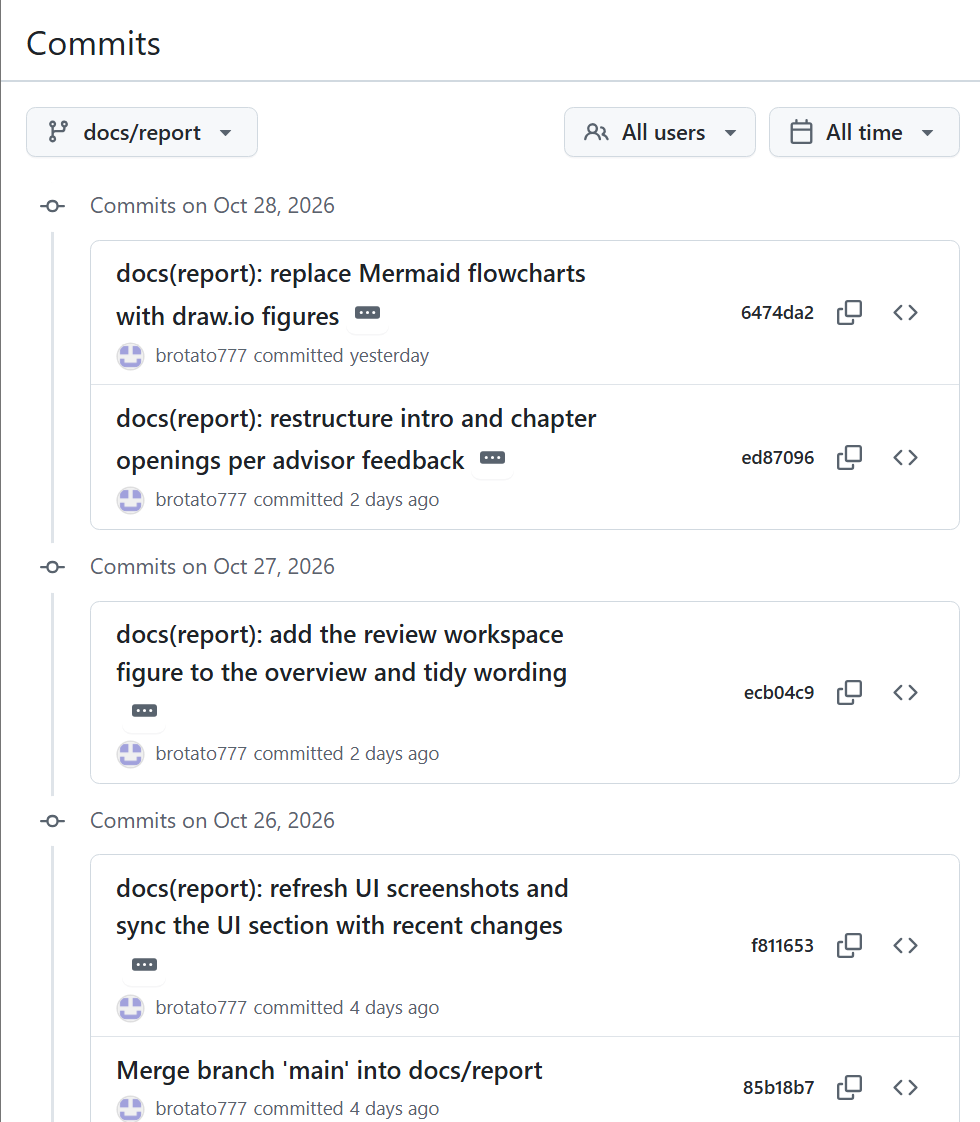
\includegraphics[width=0.45\linewidth]{project_management/github_commits_report.png}\hfill
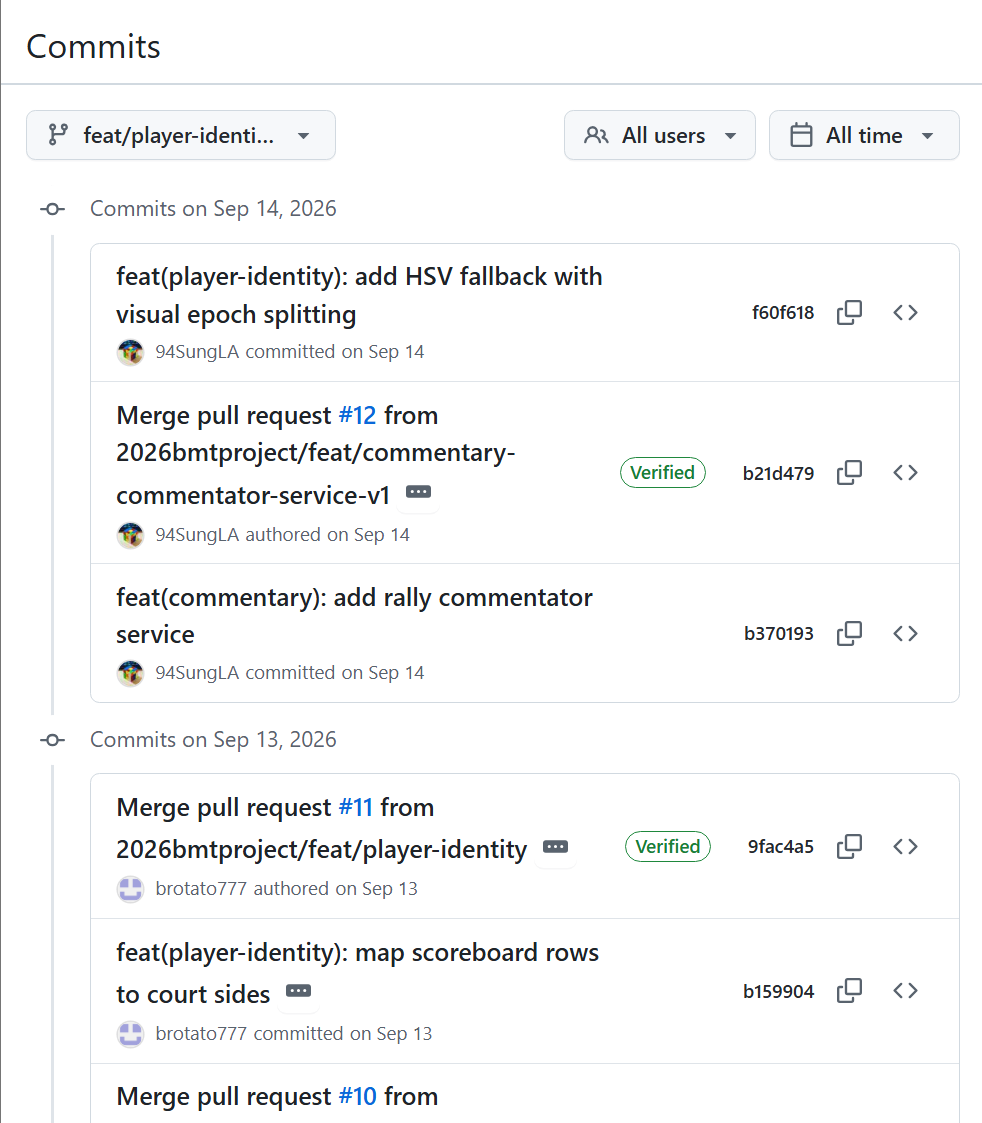
\includegraphics[width=0.45\linewidth]{project_management/github_commits_identity.png}\par
\vspace*{0.3cm}
GitHub 工作紀錄\par
\vspace*{1cm}
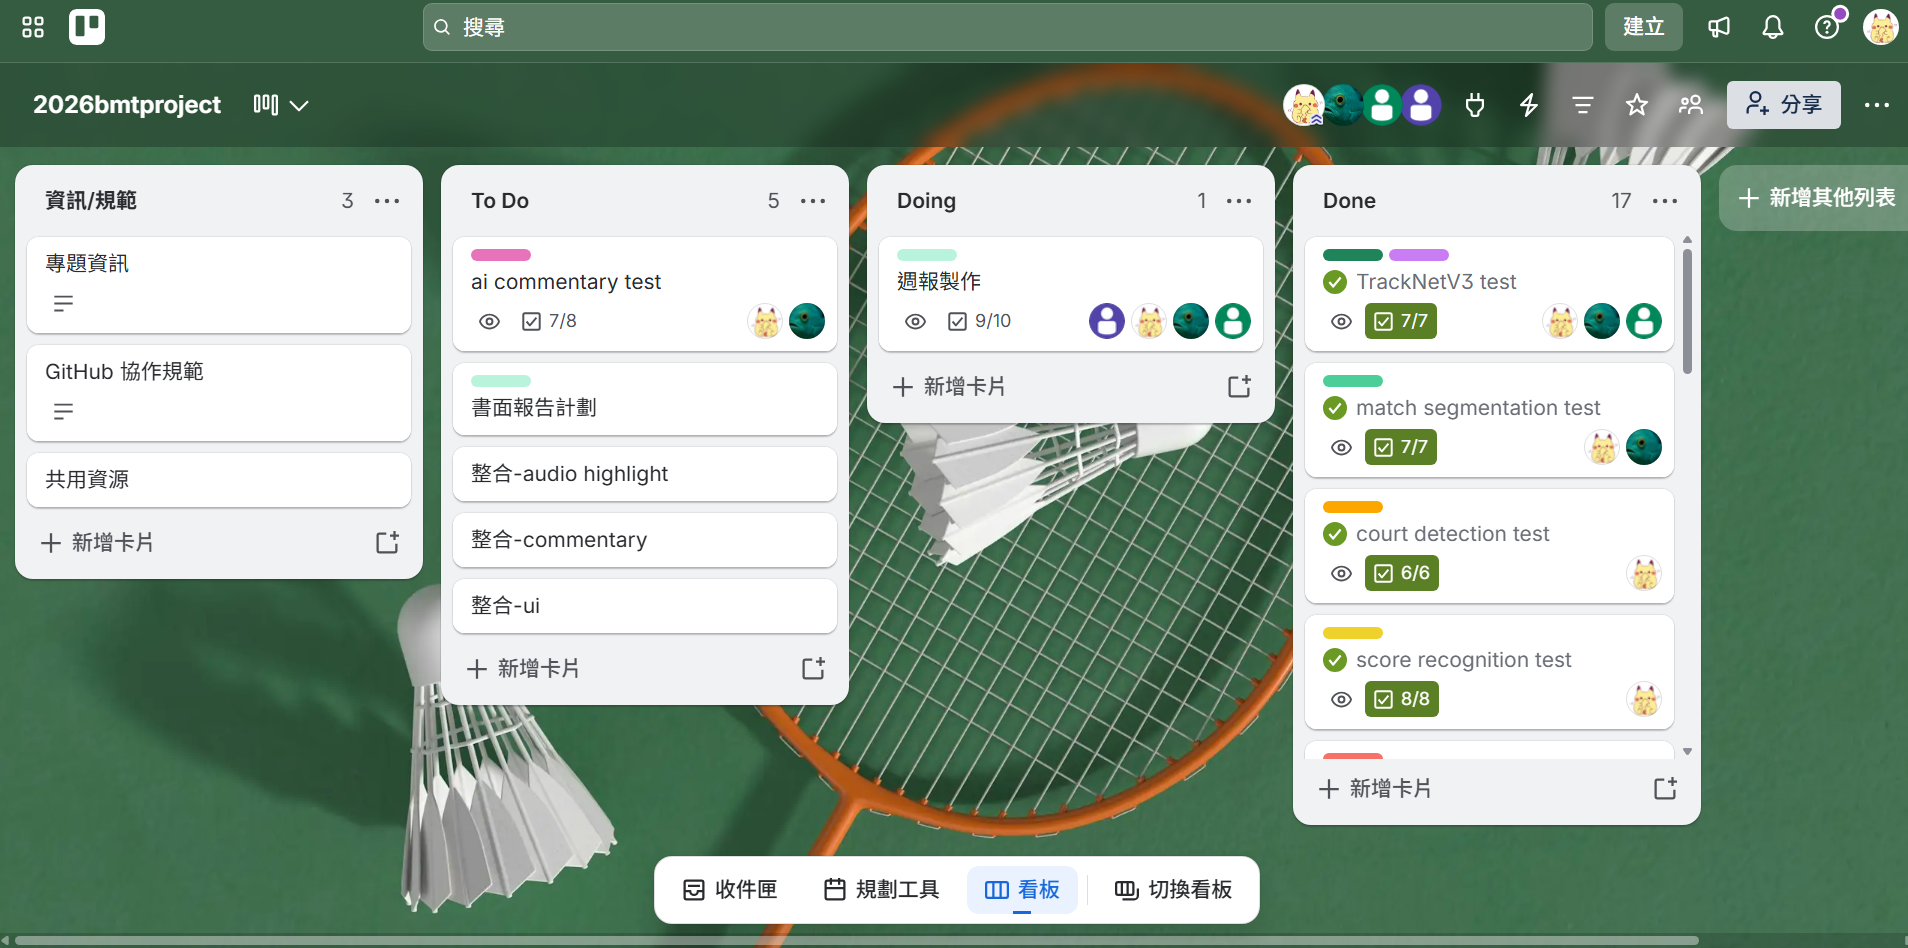
\includegraphics[width=\linewidth]{project_management/trello.png}\par
\vspace*{0.3cm}
Trello 工作紀錄\par
\end{center}

\clearpage


%%%%    【目錄區】
\tableofcontents
\listoffigures
\listoftables
\clearpage

%%%%    【摘要】從這頁開始編頁碼
\pagenumbering{arabic}
\begin{center}
\vspace*{1cm}
{\fontsize{16}{5}\selectfont\textbf{摘要}\par}
\end{center}

（待撰寫）

\clearpage


%%%%    【內文】
\chapter{簡介}
\label{ch:introduction}

\section{研究動機}
\label{sec:motivation}

羽球國際賽事的完整轉播影片大量公開於網路，記錄了選手每回合攻防的過程。教練與選手想從中歸納對手的慣用球路，研究者想統計戰術或訓練預測模型，真正需要的都不是影片本身，而是逐拍的資料，像是每回合有幾拍、每拍是什麼球種等等。影片並不直接提供這些資訊，目前仍須由人標記。ShuttleSet~\cite{shuttleset} 等羽球資料集即以人工標記建立，自動定位擊球影格的研究~\cite{chien2023hitframe} 也以減少這類人工作業為出發點。

在嘗試將既有方法套用於完整轉播影片時，我們發現學術上的單項方法大多預設輸入已經整理好，例如球種分類需要已知的擊球時刻與球場範圍。這些前提在資料集中由人工標記提供，面對一支未經處理的轉播影片時卻無從取得。要讓所有分析在真實影片上運作，就必須將它所依賴的上游步驟自動化。

因此，本專題欲補足從「原始轉播影片」到「逐拍資料」之間的落差，使後續的戰術分析、賽事理解與資料驅動應用，能建立在可由真實轉播影片取得的資料之上。

\section{專題目標}
\label{sec:goals}

本專題旨在建立一套可批次執行的全自動分析管線，將一場完整、未經人工標記的羽球單打轉播影片，轉換為可供檢索、統計與後續應用的資料，並以賽評生成與精彩片段排序兩項延伸應用，示範管線產出的用途。

\begin{itemize}
  \item \textbf{輸入}：一支完整、未經剪輯的羽球單打轉播影片，比賽中的畫面以固定俯拍的主機位為主，即 BWF 國際賽事的常見轉播形式。
  \item \textbf{輸出}：整場比賽的逐拍資料，包括每個主機位比賽片段在影片中的起訖時間與比分，片段內每一拍的擊球影格、擊球者與球種，以及雙方球員的骨架、球場範圍與羽球軌跡。可選擇另外執行賽評生成與精彩片段排序。
  \item \textbf{運作方式}：賽後批次處理，單機一張消費級 GPU 即可執行。除比分辨識與賽評需呼叫外部 API 外，其餘皆在本機完成，影片本身不需上傳。
\end{itemize}

\textbf{非本專題目標}：雙打、即時轉播分析，以及取代 Hawk-Eye 等需專用攝影設備的電子判決系統。

\section{系統概觀}
\label{sec:overview}

\begin{figure}[H]
  \centering
  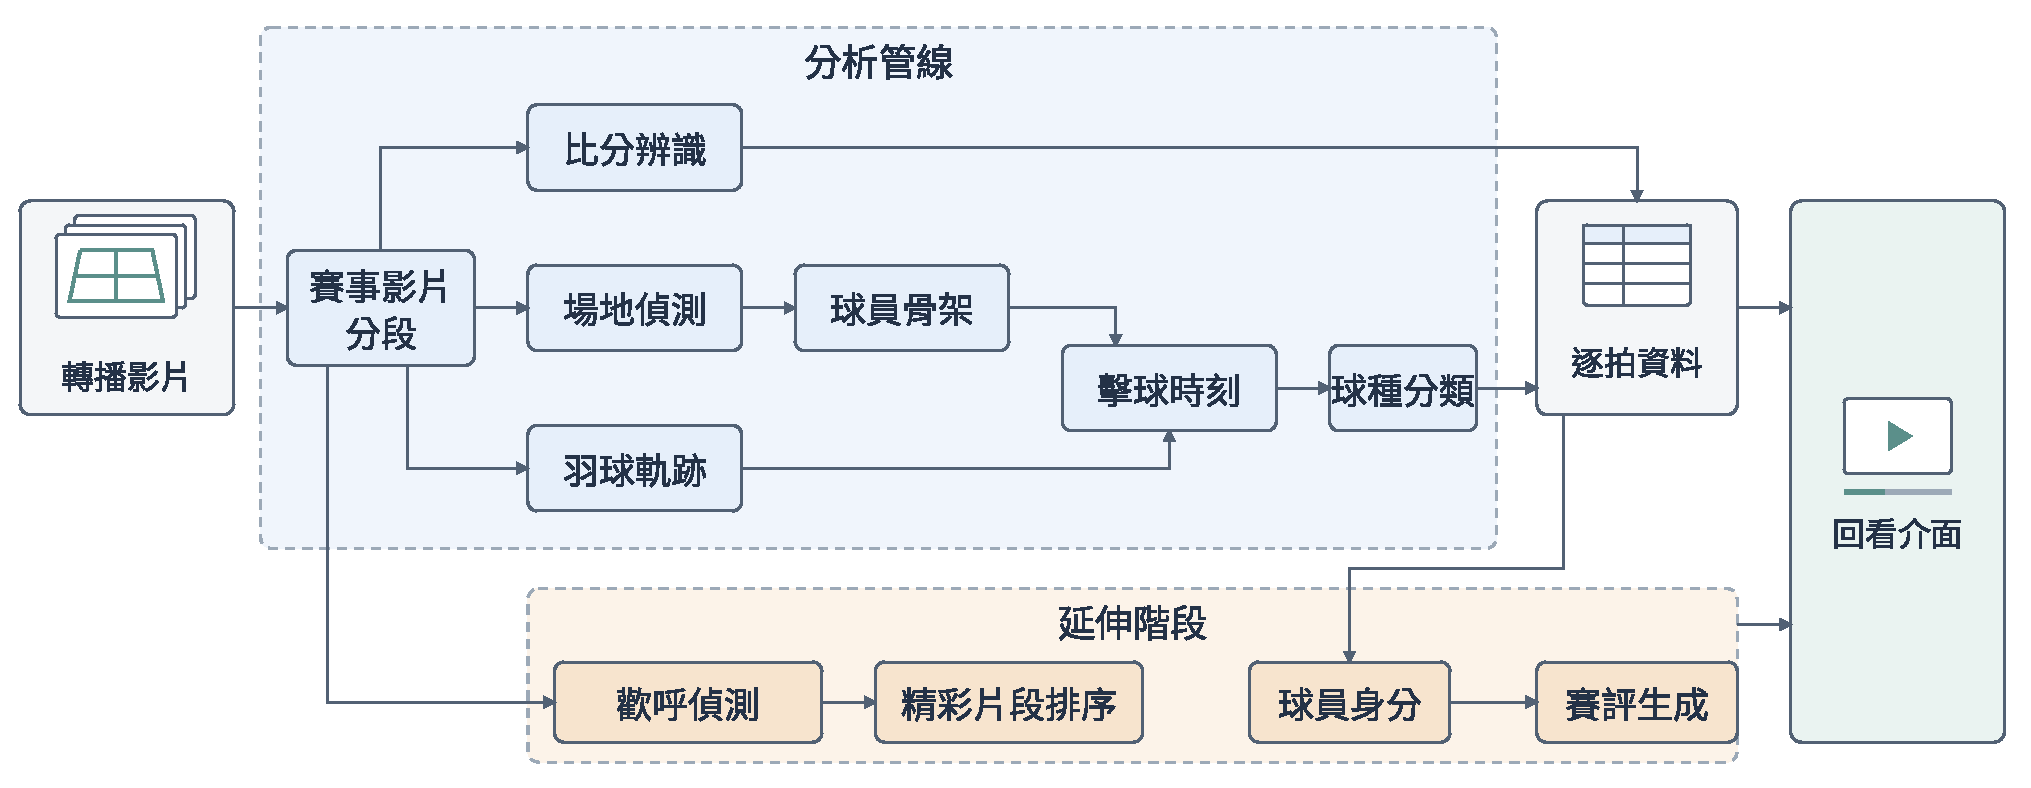
\includegraphics[scale=\flowscale]{system-overview.pdf}
  \caption[系統概觀]{系統概觀。分析管線將轉播影片轉為逐拍資料，延伸階段與回看介面建立在其產出之上。}
  \label{fig:system-overview}
\end{figure}

系統由三部分組成（\figref{fig:system-overview}）：把轉播影片轉成逐拍資料的分析管線、建立在管線產出之上的延伸階段，以及對照影片檢視結果的回看介面。分析管線依序處理以下步驟：

\begin{enumerate}
  \item \textbf{界定分析範圍。}轉播影片中夾雜重播、特寫等畫面，賽事影片分段先找出主機位的比賽片段，後續所有分析都只在這些片段內進行。比分辨識再讀出每個片段計分板上的比分，讓片段能對應回比賽中的比分。
  \item \textbf{定位球場、球員與羽球。}場地偵測定位球場範圍，建立畫面與球場平面之間的對應。球員骨架追蹤據此從裁判、線審與觀眾之中挑出場上的兩名球員。球體追蹤則逐影格定位羽球，重建羽球軌跡。這三項是後續擊球分析共同需要的輸入。
  \item \textbf{找出每一拍並分類。}擊球時刻偵測結合羽球軌跡與球員骨架，找出每一次擊球的影格。球種分類再依每一拍前後的骨架、軌跡與球場位置，判斷球種。
\end{enumerate}

管線之外另有四個延伸階段。球員身分對應依比分與發球者，把上下方對應到具體選手。賽評生成再以逐拍結果與球員身分為事實依據，由大型語言模型撰寫賽評，並逐句檢查是否有資料支持。歡呼偵測量測每個片段結束前後的觀眾歡呼，精彩片段排序據此為片段排出精彩程度。

回看介面（\figref{fig:review-workspace}）除了對照影片檢視所有結果，也能直接發起分析任務。各模組的設計與實作見\chapref{ch:system-design}。

\begin{figure}[H]
  \centering
  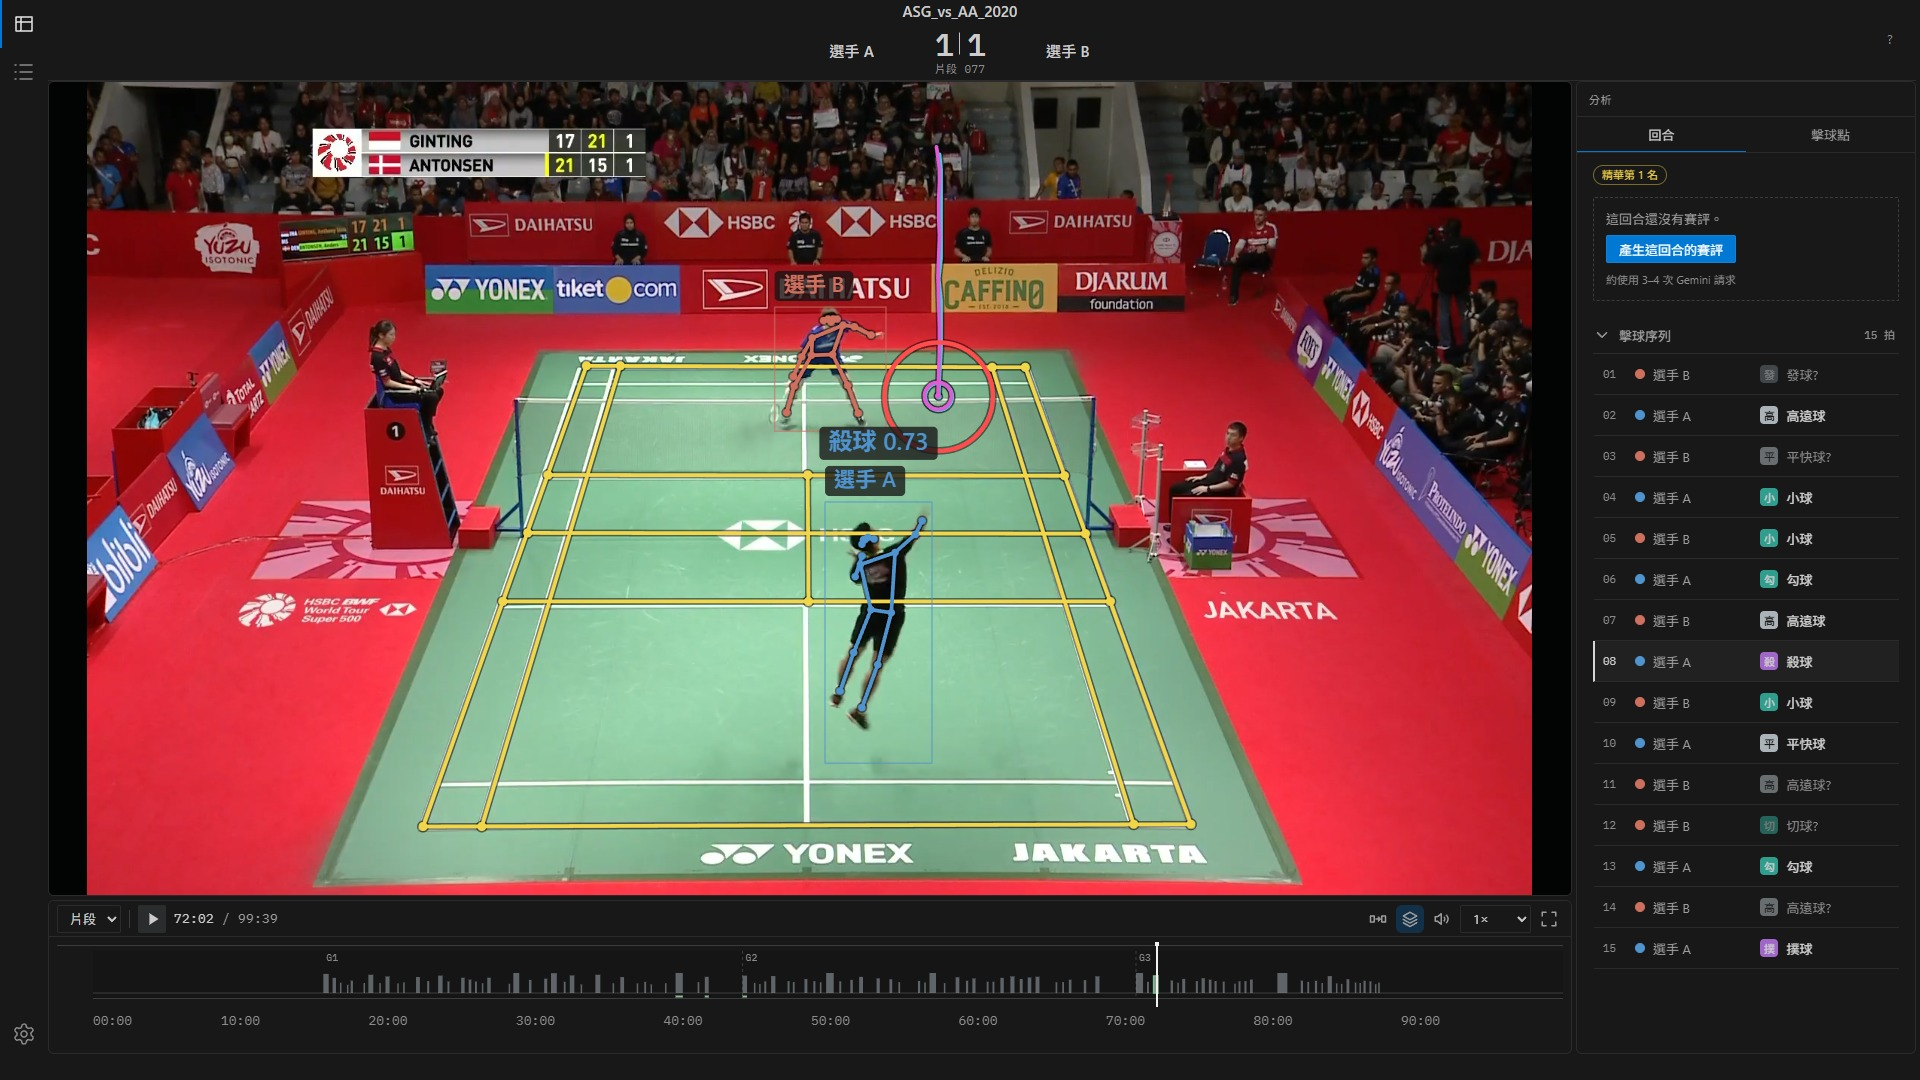
\includegraphics[width=\linewidth]{ui/review_workspace_clean.jpg}
  \caption{回看介面}
  \label{fig:review-workspace}
\end{figure}

\section{主要貢獻}
\label{sec:contributions}

上述各模組多有既有方法可以參考，但如\secref{sec:motivation}所述，這些方法預設輸入已經整理好，比賽片段起訖、球場範圍與擊球時刻都由人工提供。與既有的整合系統及開源專案相比，本系統的主要貢獻有以下四點。

\begin{enumerate}
  \item \textbf{把既有方法所依賴的上游自動化。}比賽片段起訖、球場範圍與擊球時刻在資料集中原由人工提供，本系統分別以影格差異訊號分段、由內部線條反推範圍的場地偵測，以及融合軌跡、骨架與球種證據的擊球時刻偵測取得，不需針對每支影片人工標記或調整參數。TrackNetV3~\cite{tracknetv3}、BST~\cite{bst} 等既有模型因此能直接在未經處理的轉播影片上運作。
  \item \textbf{模組化、可局部重跑的管線。}各模組仍在持續改進，因此每個階段都能單獨替換與重跑。階段之間只透過統一的資料契約溝通，執行器以上游產物的內容雜湊判斷結果是否過期，中間結果以片段為單位快取。調整其中一個模組時，只需重算受影響的部分。
  \item \textbf{公開、可重現的評估。}實驗使用 16 支 YouTube 公開的單打完整轉播，以影片為單位切分為開發集與測試集。我們公開每支影片的雜湊與影格指紋，讓他人能確認自己下載的影片與我們標記時所用的一致。真值、評分程式與逐場結果也一併公開。
  \item \textbf{應用示範：以比賽事實約束生成式 AI 的賽評。}為展示逐拍資料的下游價值，我們在管線之上建立賽評生成，重點在於避免大型語言模型的幻覺。每一拍的時刻、擊球者與球種都取自管線結果，模型只負責措辭，產生的賽評再經審查比對分析結果，沒有資料支持的句子改以只陳述事實的模板句取代。
\end{enumerate}

\section{效能評估結果}
\label{sec:results-summary}

\tabref{tab:results-summary}列出各模組的代表指標，完整實驗與失敗案例分析見\chapref{ch:experiments}。

\begin{table}[H]
  \centering
  \small
  \caption{各模組的代表指標}
  \label{tab:results-summary}
  \begin{tabularx}{\linewidth}{|l|L|l|L|}
    \hline
    模組 & 評估資料 & 主要指標 & 其他指標 \\ \hline
    賽事影片分段 & 測試集 9 場、670 個片段 & F1 98.66\%（IoU $\geq$ 0.9） & 邊界誤差中位數 0 影格 \\ \hline
    場地偵測 & 測試集 9 場、36 個外角 & 命中率 72.22\% & 誤差中位數 2.79 像素，6 場四角全中 \\ \hline
    擊球時刻偵測 & 測試集 8 場、6,990 拍 & F1 93.14\%（$\pm$5 影格） & Precision 95.49\%、Recall 90.90\% \\ \hline
    歡呼偵測 & 開發用 4 場逐場留一，外部 1 場 & Macro F1 82.70\% & ROC-AUC 0.96 \\ \hline
    處理時間 & 5 場、片長 332 分（片段 98 分） & 片段總長的 2.71 倍 & 扣除 API 等待後 1.96 倍（RTX 3060 Ti） \\ \hline
  \end{tabularx}
\end{table}

分段與擊球時刻偵測的 F1 皆超過 93\%，已可直接供下游使用。最弱的一環是場地偵測，未命中的角幾乎都源於底線旁的廣告字樣，且系統目前無法自行察覺。16 支影片中有 15 支來自 BWF 官方轉播，跨轉播單位的泛化尚未驗證。歡呼偵測僅以 4 場開發比賽與 1 場外部驗證評估。處理時間未計入音訊、身分對應與賽評等延伸階段。

\section{報告組織}
\label{sec:organization}

本報告其餘章節安排如下。\chapref{ch:related-work}回顧既有的整合系統與各子任務的方法，歸納研究缺口與本系統的定位。\chapref{ch:system-design}先說明管線架構與階段間的約定，再依處理順序介紹各模組的設計，包括影片前處理、場景與人體理解、球體分析、音訊與精彩度分析、賽事理解，最後介紹使用者介面。\chapref{ch:experiments}說明資料集與重現方式，報告各模組與端到端的實驗結果。\chapref{ch:conclusion}討論系統的優點與限制，並總結本專題與未來工作。附錄說明開發過程中生成式 AI 的使用方式。

\chapter{文獻探討}
\label{ch:related-work}

本章回答一個問題：既有整合系統能否把一支未經處理的轉播影片，自動轉換為逐拍資料？如果不能，卡在哪些環節？回顧範圍限於以單一轉播視角影片為輸入的方法。我們先在系統層級比較既有的整合系統與開源專案各自自動化了哪些環節，再逐一檢視這些環節的既有方法與前提，最後收斂出研究缺口與本系統的定位。

\section{系統層級的比較}
\label{sec:system-comparison}

要從轉播影片取得逐拍資料，最直接的方式是使用現成的整合系統。\tabref{tab:system-comparison}依本系統面對的子任務，比較五個學術整合系統與三個 GitHub 開源專案在各環節的做法。開源專案的內容以其 README 與程式碼的描述為準。

沒有一個系統能不經人工，從原始轉播一路產出逐拍資料。回合範圍常由資料集或使用者提供~\cite{guo2025coach,monotrack,rallylens}，或需由使用者選定參考畫面、模板~\cite{bosi2021thesis,rallylive}。能自動切割回合的系統，則以人工標記的資料訓練分類器~\cite{chien2023hitframe,ghosh2018structured}。比分方面，沒有系統直接讀取計分板，最多只推算回合勝方~\cite{guo2025coach,ghosh2018structured}。

三個開源專案都沒有提供任何準確率等量化評估，結果是否可靠無從判斷~\cite{rallylens,visionai,rallylive}。

文字報告方面，RallyLens 以 Gemini 生成回合分析報告，並讓數字全由程式計算、模型只負責詮釋，以避免數字幻覺~\cite{rallylens}。

\begin{table}[H]
  \centering
  \footnotesize
  \setlength{\tabcolsep}{3.5pt}
  \caption{既有整合系統與開源專案在各子任務的做法}
  \label{tab:system-comparison}
  \begin{tabularx}{\linewidth}{|>{\raggedright\arraybackslash\hyphenpenalty=10000}p{6.6em}|L|L|L|L|L|L|>{\centering\arraybackslash}p{2.2em}|}
    \hline
    {系統} & {輸入} & {回合切割} & {球場偵測} & {擊球偵測} & {球種辨識} & {比分} & {量化評估} \\
    \hline
    \multicolumn{8}{|l|}{\textbf{學術整合系統}} \\
    \hline
    Ghosh 等人~\cite{ghosh2018structured} & 完整比賽 & HOG＋SVM & 未說明 & 無 & TCN 逐幀動作分段 & 由發球者推算勝方 & 有 \\
    \hline
    Chien 與 Yu~\cite{chien2023hitframe} & 完整比賽 & CNN 分類拍攝角度 & Court R-CNN & 姿態 Transformer & 無 & 無 & 有 \\
    \hline
    Bosi~\cite{bosi2021thesis} & 完整比賽 & 與使用者選定的參考畫面比對 & 使用者點選四角 & 軌跡幾何＋音訊 & 無 & 列為目標但未實現 & 有 \\
    \hline
    MonoTrack~\cite{monotrack} & 回合片段 & 無 & 幾何式 & HitNet & 無 & 無 & 有 \\
    \hline
    Guo 等人~\cite{guo2025coach} & 回合片段 & 無 & Hough 幾何式 & 擊球者切換＋羽球角度 & 手工特徵＋邏輯迴歸 & 只判回合勝方 & 有 \\
    \hline
    \multicolumn{8}{|l|}{\textbf{GitHub 開源專案}} \\
    \hline
    RallyLens~\cite{rallylens} & 使用者截取的片段 & 無 & Hough 自動，可人工點選 & 手腕與羽球距離規則 & 無 & 無 & 無 \\
    \hline
    Badminton-VisionAI~\cite{visionai} & 完整比賽 & README 稱自動，未說明方法 & 預設讀取固定關鍵點檔 & 未說明 & Roboflow 雲端模型 & 無 & 無 \\
    \hline
    RallyLive~\cite{rallylive} & 完整比賽或直播串流 & 與使用者選定的球場模板比對 & 比對白／黃場線模型，可人工修正 & 實驗功能 & 無 & 無 & 無 \\
    \hline
  \end{tabularx}
\end{table}

\section{關鍵子任務的既有方法}
\label{sec:subtask-methods}

\subsection{回合切割}

既有方法多利用「回合進行時，轉播固定以俯拍主機位拍攝」的慣例，把回合切割化約為逐幀判斷是否為比賽畫面。一類是監督式分類，Ghosh 等人以 HOG 特徵搭配 SVM 分類，再以 Kalman 濾波平滑~\cite{ghosh2018structured}。Chien 與 Yu 以 CNN 分類拍攝角度，單幀準確率達 99.76\%，換算成回合後 F1 卻只有 89.27\%，作者歸因於轉播鏡頭形式多變~\cite{chien2023hitframe}。另一類是與參考畫面比對，Bosi 計算每幀與使用者選定之參考畫面的 RGB 差與 PSNR，以經驗門檻判斷~\cite{bosi2021thesis}。

\subsection{球場偵測}

學習式方法以標記資料訓練場地關鍵點偵測器，例如以 Court R-CNN 輸出單打場地的 6 個關鍵點~\cite{chien2023hitframe}，或以 YOLO 架構偵測 14 個場地地標~\cite{singha2025hybrid}。幾何式方法利用場線結構與已知尺寸，不需訓練。AI-Powered Badminton Coach 以 Hough 直線取得候選線，再做透視校正~\cite{guo2025coach}。MonoTrack 把標準球場模型對到候選線上，並指出原演算法寫死的角度門檻使約四分之一的影片失敗，改良後成功率由 73.9\% 提升至 85.5\%~\cite{monotrack}。Bosi 的系統則由使用者人工點出球場四角~\cite{bosi2021thesis}。

\subsection{球體追蹤}

羽球小、快且常被遮擋，既有方法分為熱圖式與偵測框式兩條路線。熱圖式以 TrackNet 家族為代表，輸入連續數幀、輸出標示球位置的熱圖~\cite{tracknet}。TrackNetV2 被多個整合系統直接採用~\cite{guo2025coach,bosi2021thesis}，TrackNetV3 再加入背景估計與 inpainting 軌跡修補~\cite{tracknetv3}。偵測框式如 Singha 等人修改 YOLOv8，移除大物件偵測頭以強化小物件偵測~\cite{singha2025hybrid}。此外，多數系統另以 ARIMA、內插等後處理修正軌跡~\cite{guo2025coach,bosi2021thesis}。

\subsection{擊球偵測}

既有方法依所用訊號可分為四種思路：

\begin{enumerate}
  \item \textbf{軌跡幾何。}在球的 Y 座標找峰值、X 座標找極值~\cite{bosi2021thesis}，開源專案 SoloShuttlePose \cite{soloshuttlepose} 亦屬此類。殺球前後球的運動方向連貫，此法容易漏抓~\cite{bosi2021thesis}。
  \item \textbf{球員姿態。}以 Transformer 由雙方骨架序列預測羽球飛行方向，方向轉換處即為擊球幀。容差由 $\pm$15 收緊到 $\pm$5 幀時，F1 由 79.55\% 降至 63.92\%~\cite{chien2023hitframe}。
  \item \textbf{多源學習式。}MonoTrack 的 HitNet 以 GRU 讀取球場角點、姿態與羽球位置，逐幀判斷是否擊球，再以動態規劃施加「最短間隔、擊球者交替」約束，F1 由 0.866 提升至 0.946~\cite{monotrack}。AI-Powered Badminton Coach 先判斷擊球者並以其切換處分段，再依羽球角度變化定位擊球幀~\cite{guo2025coach}。
  \item \textbf{音訊。}以 LPC 殘差偵測擊球聲，但球評、觀眾等背景噪音使召回率不理想~\cite{bosi2021thesis}。
\end{enumerate}

\subsection{球種辨識}

既有方法的差異主要在輸入型態，AI-Powered Badminton Coach 以 131 維手工特徵搭配邏輯迴歸~\cite{guo2025coach}。Singha 等人以 SlowFast 與 TimeSformer 直接處理原始影像~\cite{singha2025hybrid}。BST 則以球員骨架、羽球軌跡與場上位置為輸入~\cite{bst}。BST 須先知道擊球時刻才能切出每一拍的片段，並依賴姿態估計、羽球追蹤與場線偵測三個既有模型的輸出~\cite{bst}。

\subsection{比分辨識}

羽球文獻中鮮少直接辨識計分板，Ghosh 等人以下一回合的發球者推算上一回合的勝方，比分只在建立資料集時由人工標記~\cite{ghosh2018structured}。AI-Powered Badminton Coach 只判斷回合勝方、不讀比分~\cite{guo2025coach}。Bosi 雖把比分列為目標，最終並未實現~\cite{bosi2021thesis}。網球的 SmartTennisTV 自動定位計分板後以 OCR 辨識，再以計分規則修正錯誤，但指出 Tesseract 需依賽事人工設定前處理~\cite{smarttennistv}。

\section{研究缺口與本系統定位}
\label{sec:research-gap}

綜合前兩節，既有工作仍有兩項缺口。第一，沒有系統能從原始轉播影片一路自動產出逐拍資料。回合範圍、球場位置等上游前提多由資料集或使用者提供，也尚無系統直接讀取計分板，連 HitNet、BST 等較強的模型也假設這些輸入已經就緒。第二，已經自動化的環節多需以逐幀或場地標記訓練，換賽事、換轉播形式就可能失準。開源專案則普遍沒有量化評估，難以判斷結果是否可靠。

本系統定位為一條批次執行的分析管線。上游步驟不需另外訓練模型，也不需針對每支影片人工標記或調整參數，讓既有的成熟模型能直接用在未經處理的轉播影片上，並以公開的真值與評分程式評估各模組。在此基礎上再產生精彩片段排序與自然語言賽評。各子任務的路線如\tabref{tab:positioning}。

\begin{table}[H]
  \centering
  \small
  \caption{本系統在各子任務採用的路線}
  \label{tab:positioning}
  \begin{tabularx}{\linewidth}{|l|L|r|}
    \hline
    {子任務} & {本系統的路線} & {詳見} \\ \hline
    回合切割 & 影格差異訊號，門檻由影片自身分布估計 & \secref{sec:match-segmentation} \\ \hline
    比分辨識 & VLM 轉錄計分板 & \secref{sec:score-recognition} \\ \hline
    球場偵測 & 幾何式，不預設球場顏色，由內部場線反推球場範圍 & \secref{sec:court-detection} \\ \hline
    球體追蹤 & 預訓練 TrackNetV3，加上多候選 Viterbi 後處理 & \secref{sec:shuttle-tracking} \\ \hline
    擊球偵測 & 融合軌跡、骨架與球種模型，以結構約束補漏拍 & \secref{sec:hit-detection} \\ \hline
    球種分類 & 預訓練 BST & \secref{sec:stroke-classification} \\ \hline
    歡呼偵測 & YAMNet 特徵辨識觀眾歡呼，作為精彩度訊號 & \secref{sec:cheer-audio} \\ \hline
  \end{tabularx}
\end{table}

\chapter{系統設計}
\label{ch:system-design}

本章說明系統各部分的設計與實作。\secref{sec:architecture}先介紹整體架構，包括各階段的相依關係、產物，以及讓各階段能單獨開發與重跑的管線約定。接著依功能分五節介紹各模組：

\begin{itemize}
  \item \textbf{影片前處理}：賽事影片分段與比分辨識，負責界定分析範圍。
  \item \textbf{場景與人體理解}：場地偵測與球員骨架追蹤。
  \item \textbf{球體分析}：球體追蹤與軌跡重建、擊球時刻偵測與球種分類。
  \item \textbf{音訊與精彩度分析}：歡呼音訊量測與精彩片段排序。
  \item \textbf{賽事理解}：球員身分對應、賽評生成。
\end{itemize}

最後一節介紹回看介面。

各模組大致可以獨立閱讀，開頭的概述依序說明該模組要解決的問題與目標、設計重點與處理流程總覽，之後再逐步說明各步驟的細節。各模組的實驗結果集中於\chapref{ch:experiments}。

\section{系統架構}
\label{sec:architecture}

管線共有十一個階段（\figref{fig:system-architecture}），每個階段讀取上游的產物，輸出一個 JSON 產物。除分段直接讀取原始影片外，其餘階段都以 \texttt{segments.json} 界定分析範圍。各階段的相依與產物如\tabref{tab:stages}。

\begin{figure}[H]
  \centering
  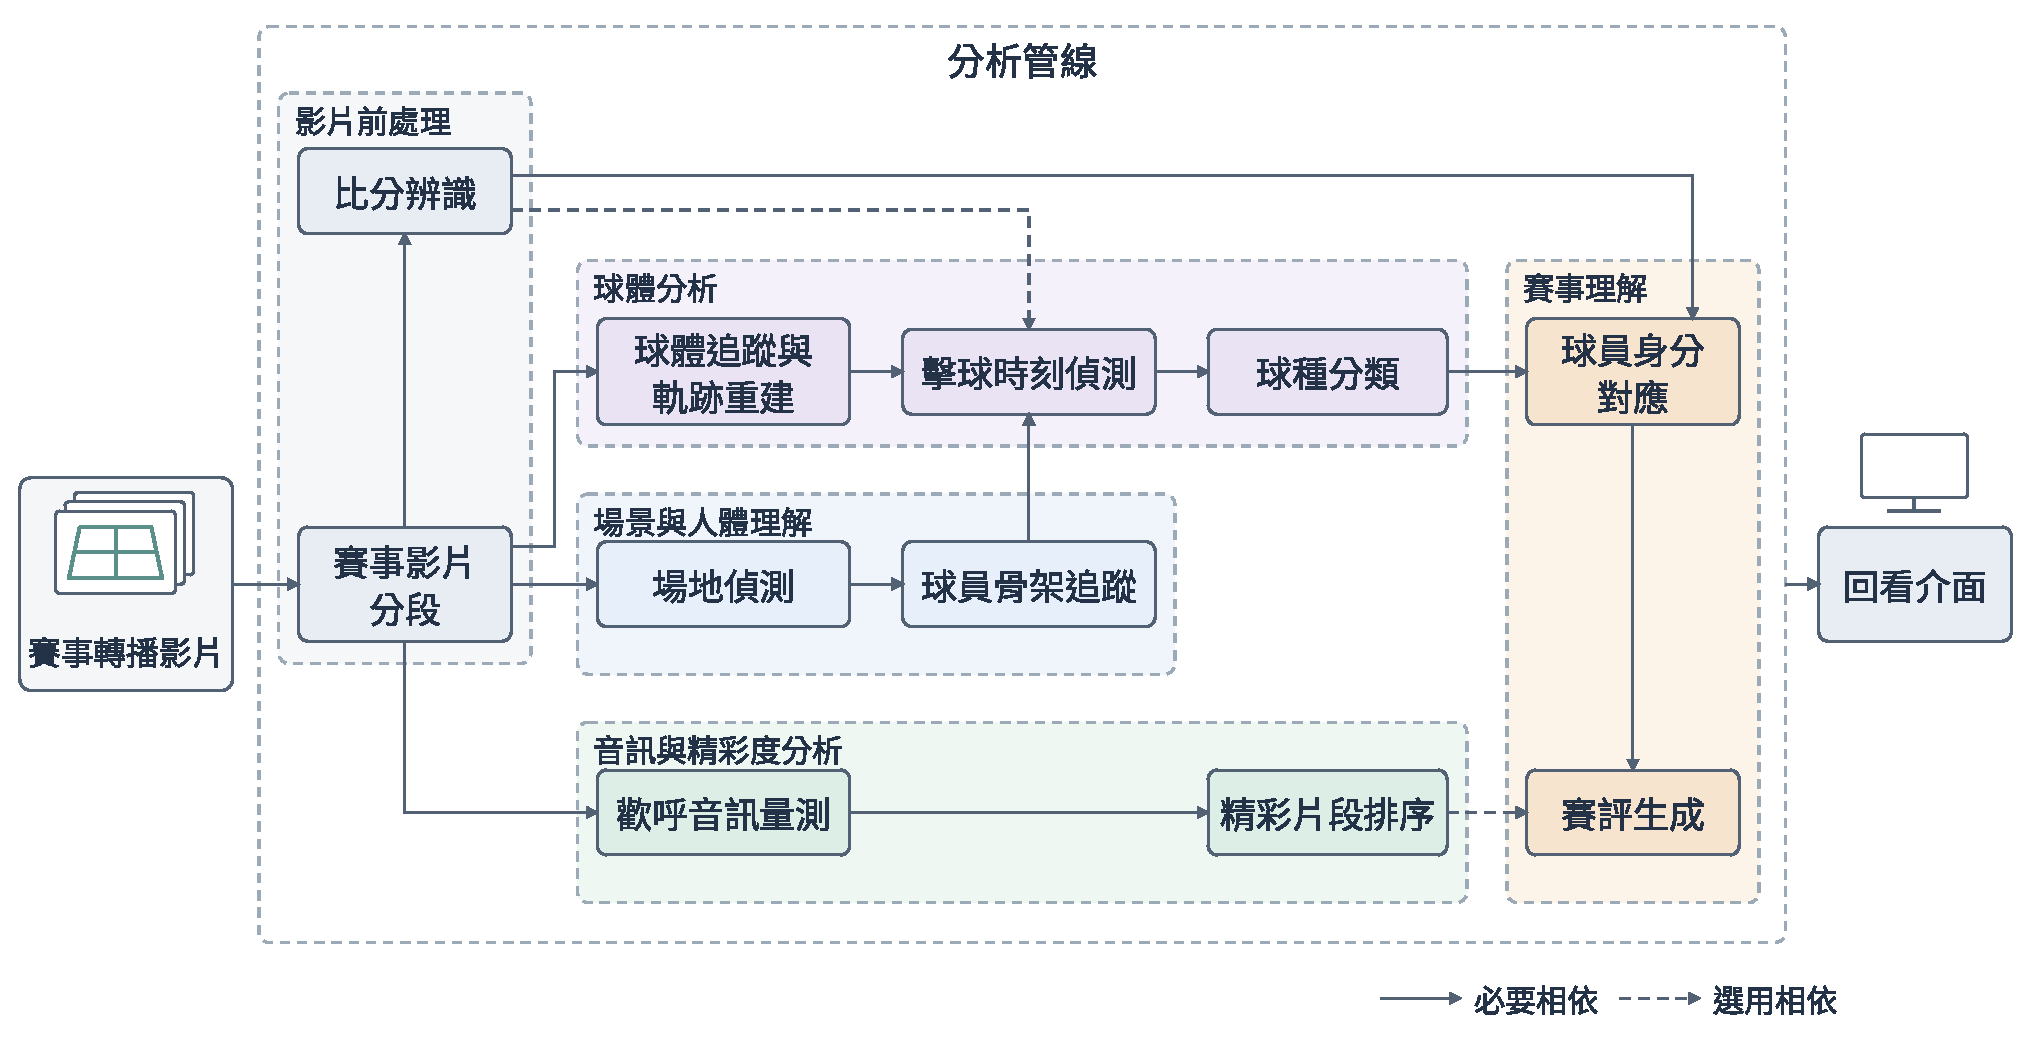
\includegraphics[scale=\flowscale]{system-architecture.pdf}
  \caption{系統架構}
  \label{fig:system-architecture}
\end{figure}

\subsection{管線約定}
\label{sec:pipeline-conventions}

以下四個約定讓各階段能各自開發、單獨執行與重跑。

\begin{enumerate}
  \item \textbf{單一產物、統一格式。}每個階段只寫一個 JSON 產物，外層固定是一個物件、內含一組記錄陣列，記錄欄位由程式中的資料類別統一定義。因為形狀一致，讀寫共用同一組函式，新增階段只需定義資料類別。
  \item \textbf{以完整比賽時間對齊。}所有產物都以原始影片的時間為準，視覺結果記錄絕對影格編號，音訊窗口記錄在整場比賽中的起訖秒數，片段層級的結果則以片段在 \texttt{segments.json} 中的索引對應。
  \item \textbf{產物與快取分離。}每場比賽的 \texttt{cache/} 放昂貴但可重建的中間結果（降解析度影片、TrackNet 熱圖、人體偵測結果、逐幀球種機率）。快取以內容命名並以片段為單位存放，因此中斷可續跑，重新分段時也只有內容改變的片段需要重算。
  \item \textbf{依內容判斷是否重跑。}使用者可只選取部分階段，執行器依相依關係排序後逐一執行，已完成的階段預設跳過。透過比對上游產物的內容雜湊判斷是否跳過。任一階段失敗即停止整條管線。
\end{enumerate}

\begin{table}[H]
  \centering
  \small
  \caption{管線各階段的相依與產物}
  \label{tab:stages}
  \begin{tabularx}{\linewidth}{|>{\raggedright\arraybackslash}p{6.2em}|>{\hsize=.85\hsize}L|>{\ttfamily\footnotesize}l|>{\hsize=1.15\hsize}L|}
    \hline
    階段 & 相依階段 & \normalfont 產物 & 每筆記錄的內容 \\ \hline
    賽事影片分段 & — & segments.json & 一個主機位比賽片段的起訖影格 \\ \hline
    比分辨識 & 分段 & scores.json & 一個片段的比分、發球方與局數；片段內含多個回合時，另記各回合比分與切點 \\ \hline
    場地偵測 & 分段 & court.json & 球場四個外角，以及球場平面與影像之間的單應矩陣 \\ \hline
    球體追蹤與軌跡重建 & 分段 & shuttle.json & 一幀中羽球的座標與可見性，兩種軌跡各一份 \\ \hline
    球員骨架追蹤 & 分段、場地偵測 & pose.json & 一幀中兩名球員的 17 個關節點與人體框 \\ \hline
    擊球時刻偵測 & 球體追蹤、骨架追蹤；選用：比分辨識 & events.json & 一次擊球的影格編號 \\ \hline
    球種分類 & 擊球時刻偵測、骨架追蹤、球體追蹤、場地偵測 & strokes.json & 一次擊球的球種（8 類）、擊球者（畫面上方或下方）與信心 \\ \hline
    歡呼音訊量測 & 分段 & audio\_signals.json & 一個片段的歡呼信心與強度，以及逐窗口的歡呼分數 \\ \hline
    精彩片段排序 & 歡呼音訊量測 & highlights.json & 一個片段的精彩度分數 \\ \hline
    球員身分對應 & 球種分類、比分辨識；選用：骨架追蹤 & identity.json & 兩次換邊之間，上下方球員各對應計分板上的哪位選手，以及判定依據 \\ \hline
    賽評生成 & 分段、擊球時刻偵測、球種分類、比分辨識、身分對應；選用：精彩片段排序、骨架追蹤、場地偵測、球體追蹤 & commentary.json & 一個片段的回合賽評與逐拍賽評 \\ \hline
  \end{tabularx}
\end{table}

\section{影片前處理}
\label{sec:preprocessing}

\subsection{賽事影片分段}
\label{sec:match-segmentation}

\subsubsection{概述}

\textbf{問題與目標：}一支羽球轉播影片中，適合進行球員、羽球軌跡分析的畫面，主要來自固定俯拍的機位。若系統直接分析整部影片，非固定機位比賽畫面會產生大量錯誤資料，也浪費運算資源。本模組從轉播影片中找出固定機位比賽畫面，作為後續模組的輸入。

\textbf{設計重點：}本模組不需額外訓練模型、標註資料，也不需針對每支影片逐片人工調整參數，依據影片的統計結構自適應於不同影片。核心設計是把「固定機位比賽畫面主要只有球員移動」這個先驗，轉化為影格差異訊號。固定機位比賽片段的相鄰影格差異小、運鏡與鏡頭切換差異大、靜止的計分板差異極小，因此只用一個廉價的差異指標（MAD）就能把固定機位比賽片段與其他畫面在數值上分開。另一個核心設計是利用「同一機位在不同片段間具有高度相似性」，排除計分板、重播及其他靜止畫面。在 9 場未參與開發的比賽上，片段偵測 F1 達 98.66\%（見\secref{sec:exp-segmentation}）。

\textbf{處理流程總覽：}如\figref{fig:match-segmentation-flow}。

\begin{figure}[H]
  \centering
  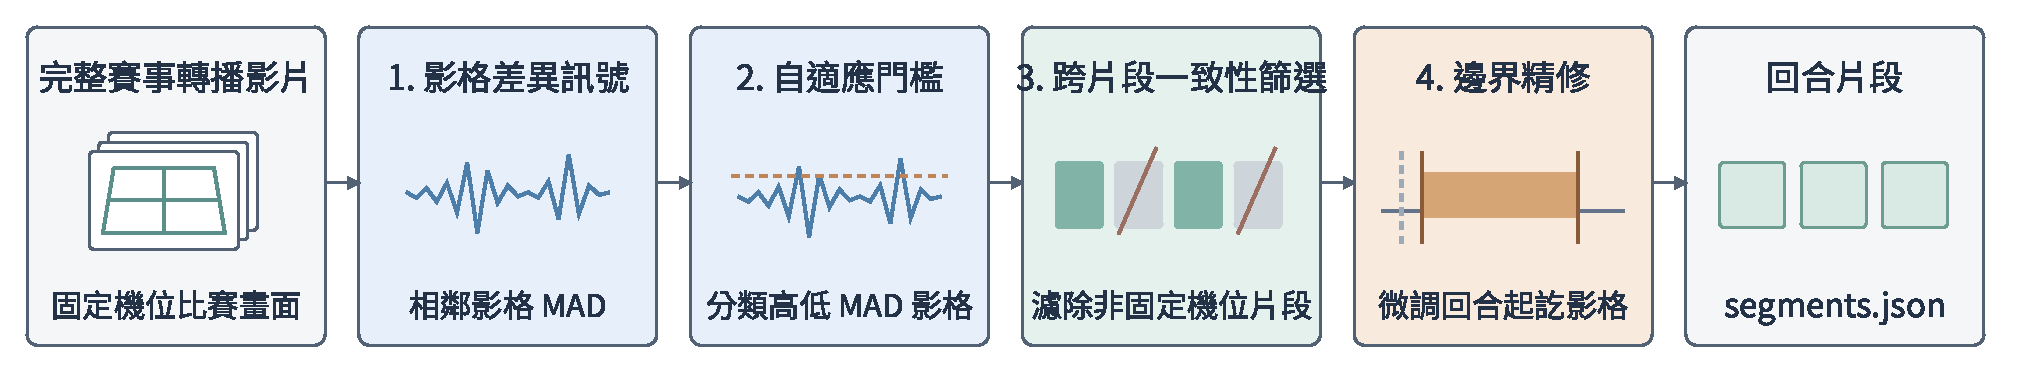
\includegraphics[scale=\flowscale]{match-segmentation.pdf}
  \caption{賽事影片分段處理流程}
  \label{fig:match-segmentation-flow}
\end{figure}

\subsubsection{影格差異訊號}

固定機位比賽片段畫面中只有兩名球員與球在動，兩影格間的差異小。其餘片段則落在兩個極端，鏡頭移動與切換使差異極大，靜止的計分板與定格畫面則差異極小。本模組以影格與影格之間的差異作為核心訊號。差異以 MAD（平均絕對差，Mean Absolute Difference）衡量：
\begin{equation}
  \mathrm{MAD} = \frac{1}{MN}\sum_{x=1}^{M}\sum_{y=1}^{N} \left| I_1(x,y) - I_2(x,y) \right|
  \label{eq:mad}
\end{equation}
其中 $M$、$N$ 為影像寬高，$I(x,y)$ 為座標 $(x,y)$ 的灰階值。選用 MAD 的理由是成本低廉、對離群值不敏感、且動態範圍足夠。計算前先將影片縮放至 480p 以減少計算量。MAD 不隨解析度改變，相對高低仍然成立。

取樣採每隔三個影格一次，並與前一個取樣影格計算 MAD。間隔取樣一方面縮短處理時間，一方面避免特寫片段和固定機位比賽片段混淆。特寫中球員動作緩慢、背景固定，MAD 偏低且接近固定機位比賽片段，間隔取樣把緩慢位移放大、拉高其 MAD。固定機位比賽片段中球員佔比小、動作劇烈，間隔取樣影響有限。兩類片段因此在 MAD 上分開。

\begin{figure}[H]
  \centering
  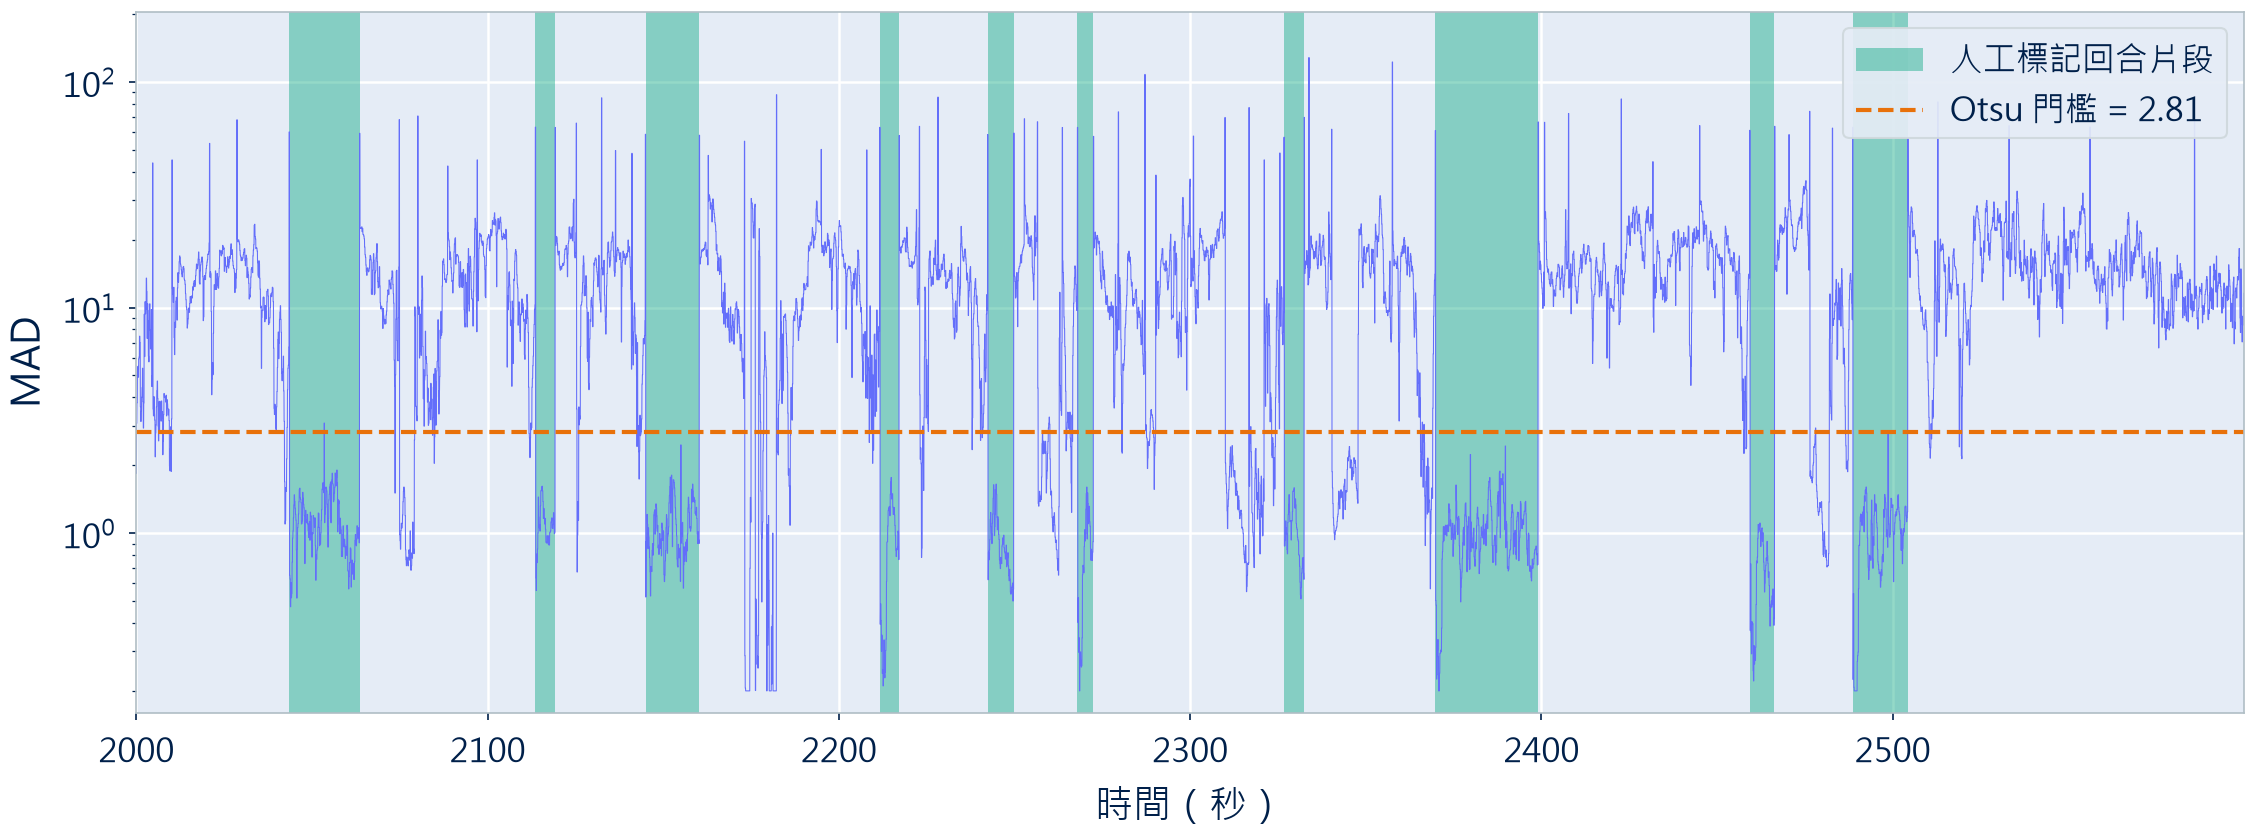
\includegraphics[width=\linewidth]{match_segmentation/mad_timeline.png}
  \caption{部分片段 MAD}
  \label{fig:mad-timeline}
\end{figure}

\figref{fig:mad-timeline}中綠色區塊為手動標記的固定機位比賽片段，虛線為系統算出的門檻，可見綠色區塊的 MAD 通常低於門檻。

\subsubsection{自適應門檻}

本階段統計全片的 MAD 分佈，設定一個門檻把影格分成低 MAD（固定機位比賽畫面、靜止畫面）與高 MAD（運鏡、鏡頭切換）。不同影片的分佈不同，門檻須隨影片自動調整。

分析前先對 MAD 取以 10 為底的對數。鏡頭切換到完全不同畫面時每個像素都不一樣，會產生極大 MAD，使分佈右側出現長尾。取對數可壓縮長尾，使高低兩側尺度相當。實作取 $\log_{10}(\max(\mathrm{MAD}, 1))$，因為 MAD 可能為 0，需要地板值 1。

\begin{figure}[H]
  \centering
  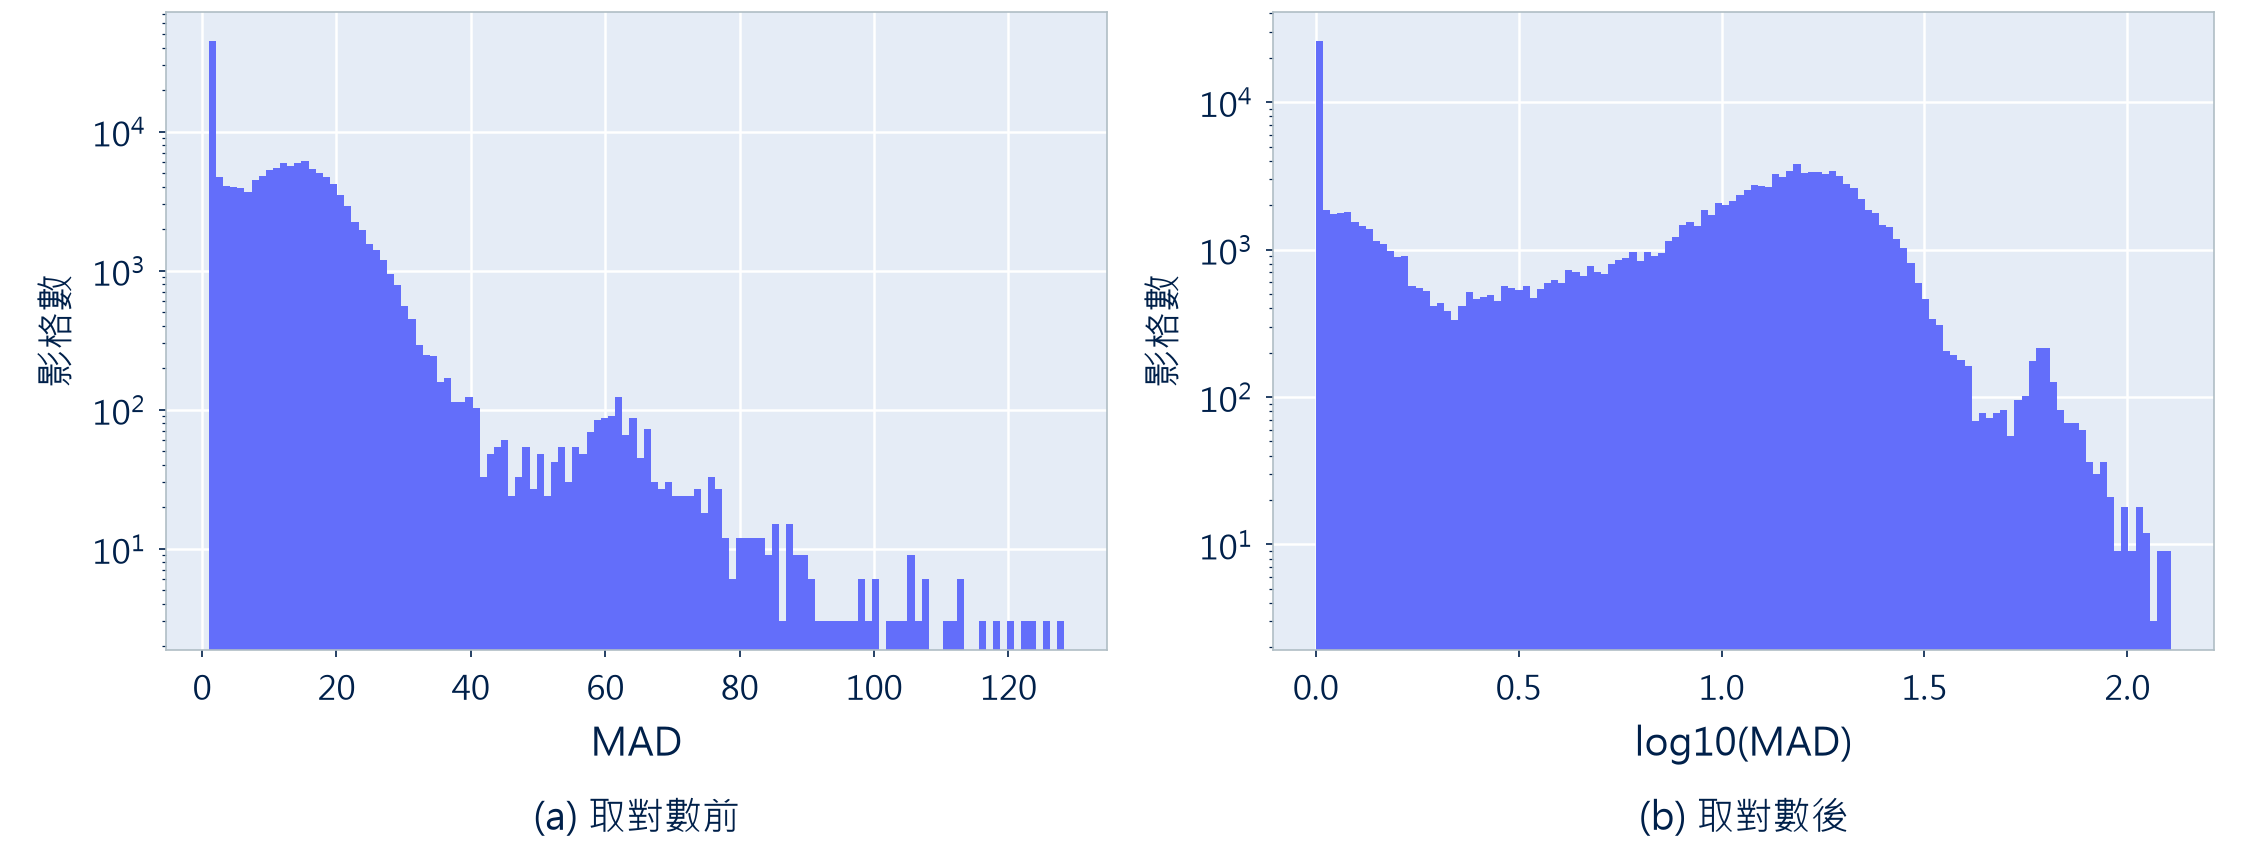
\includegraphics[width=\linewidth]{match_segmentation/log_transform.png}
  \caption{取對數}
  \label{fig:log-transform}
\end{figure}

\textbf{乾淨片段偵測：}若輸入本身無鏡頭切換，重尾程度會遠低於多鏡頭影片，據此判定乾淨固定機位片段，跳過後續步驟直接輸出。

\textbf{門檻方法：}設門檻的問題與影像二值化相似，二值化統計像素亮度並切成兩類，本階段統計影格 MAD 並切成兩類，故沿用二值化的門檻計算方法。本系統採 Otsu 法，它只要求兩類均值不同即可分離，不限制分佈形狀、不需調參，正好適用於本階段低 MAD 側有尖峰、高 MAD 側是不對稱長尾的情形。

\begin{figure}[H]
  \centering
  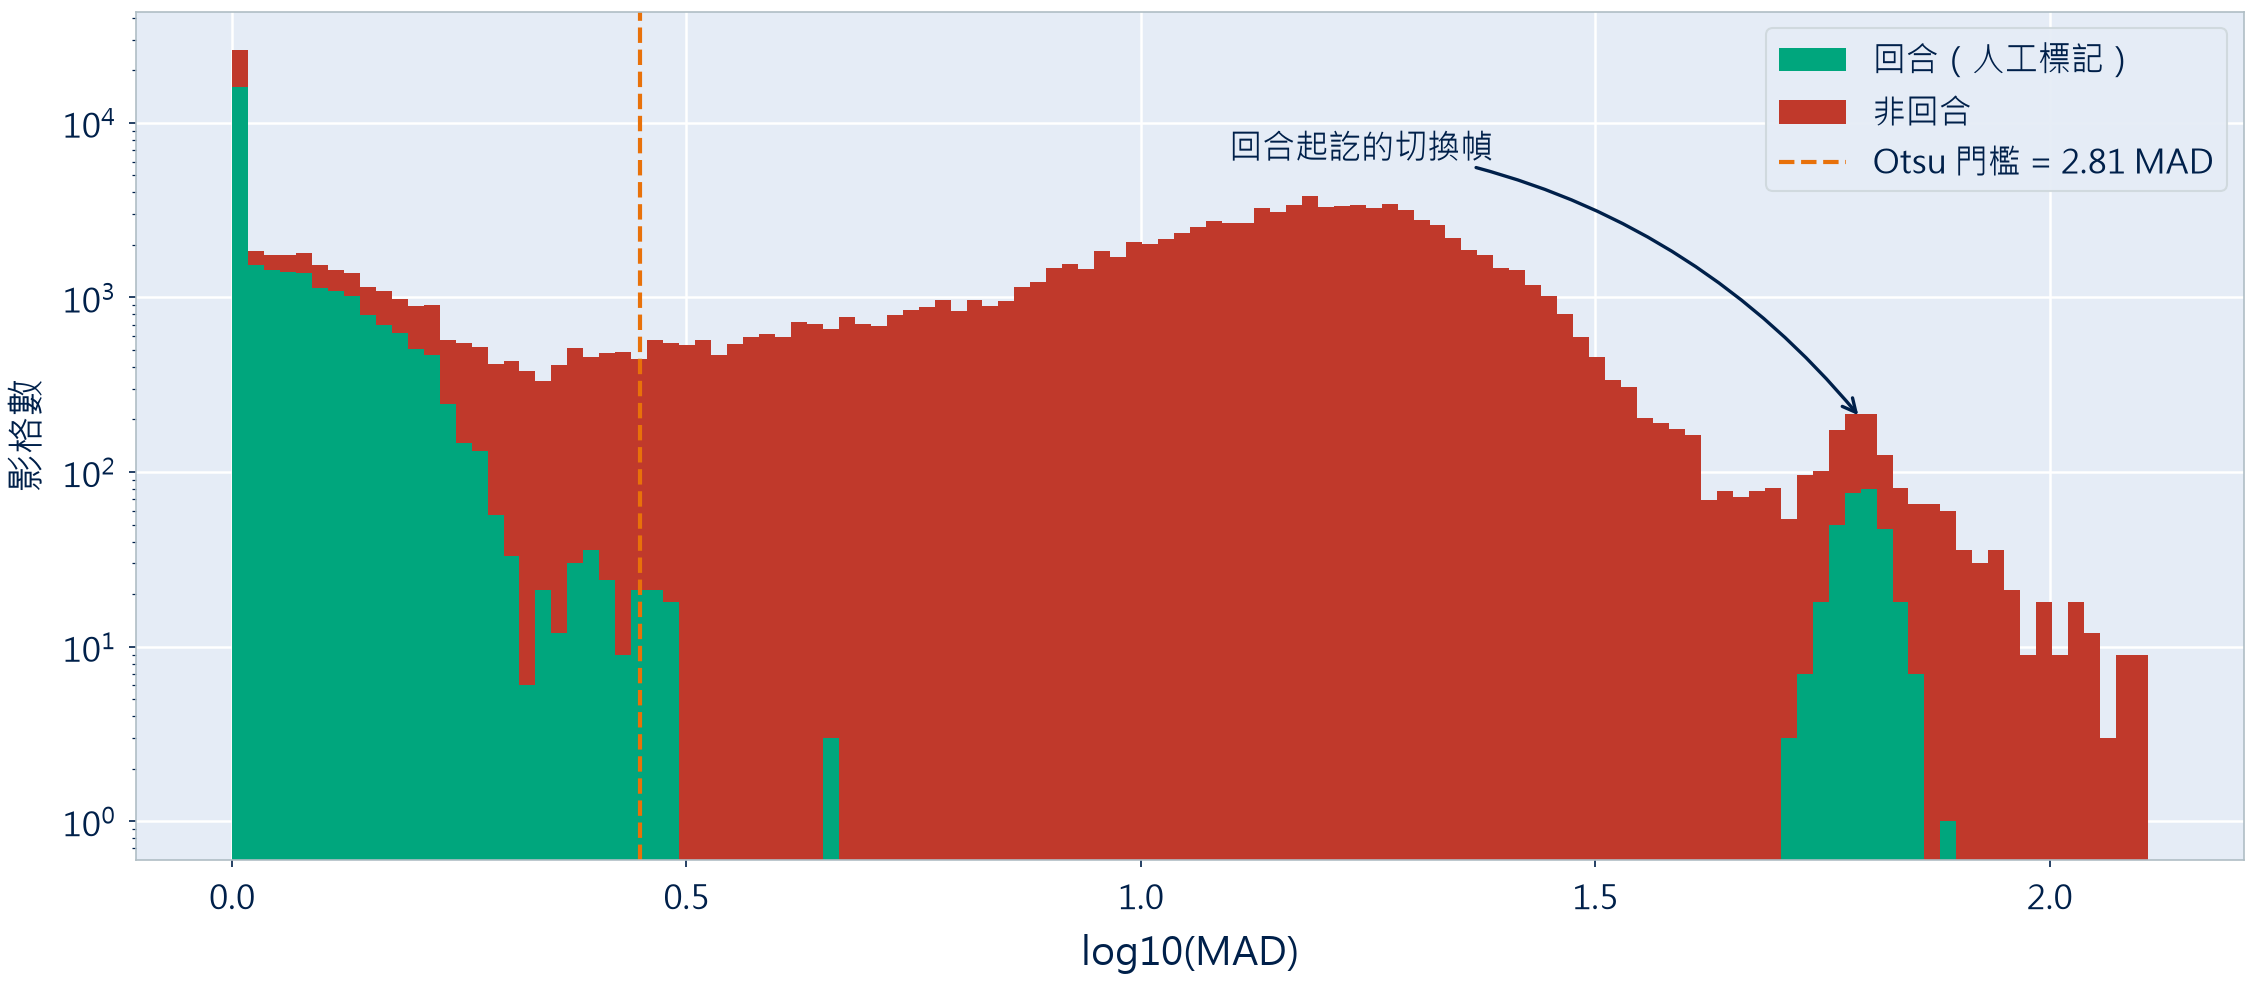
\includegraphics[width=\linewidth]{match_segmentation/rally_split_hist.png}
  \caption{固定機位比賽片段與其他片段的 MAD 分佈}
  \label{fig:rally-split-hist}
\end{figure}

\begin{table}[H]
  \centering
  \caption{$\log_{10}(\mathrm{MAD})$ 的分佈與組成}
  \label{tab:mad-composition}
  \begin{tabular}{|l|r|r|l|}
    \hline
    MAD 區間 & 佔全片比例 & 固定機位比賽比例 & 畫面性質 \\ \hline
    0--0.5 & 6.8\% & 28\% & 近乎靜止 \\ \hline
    0.5--2 & 23\% & 75\% & 固定機位比賽畫面 \\ \hline
    2--2.75 & 2.3\% & 5\% & 谷底，門檻落點 \\ \hline
    2.75--30 & 65\% & 約 0\% & 重播、運鏡 \\ \hline
    30 以上 & 2.8\% & 7\% & 快速轉場 \\ \hline
  \end{tabular}
\end{table}

\textbf{三類切分：}直接做兩類 Otsu 會產生系統性偏差，高 MAD 側佔全片 68\% 且橫跨 2.75 至 128，類內變異遠大於低 MAD 側，會把切點從谷底推進高 MAD 團內部，讓大量非固定機位比賽影格進入下一步。改用三類切分，上切點（10.80）吸收長尾壓力，下切點（2.81）回到谷底，取下切點為門檻（\figref{fig:otsu-3class}）。三類 Otsu 的效果等價於先移除長尾再做兩類 Otsu。

\begin{figure}[H]
  \centering
  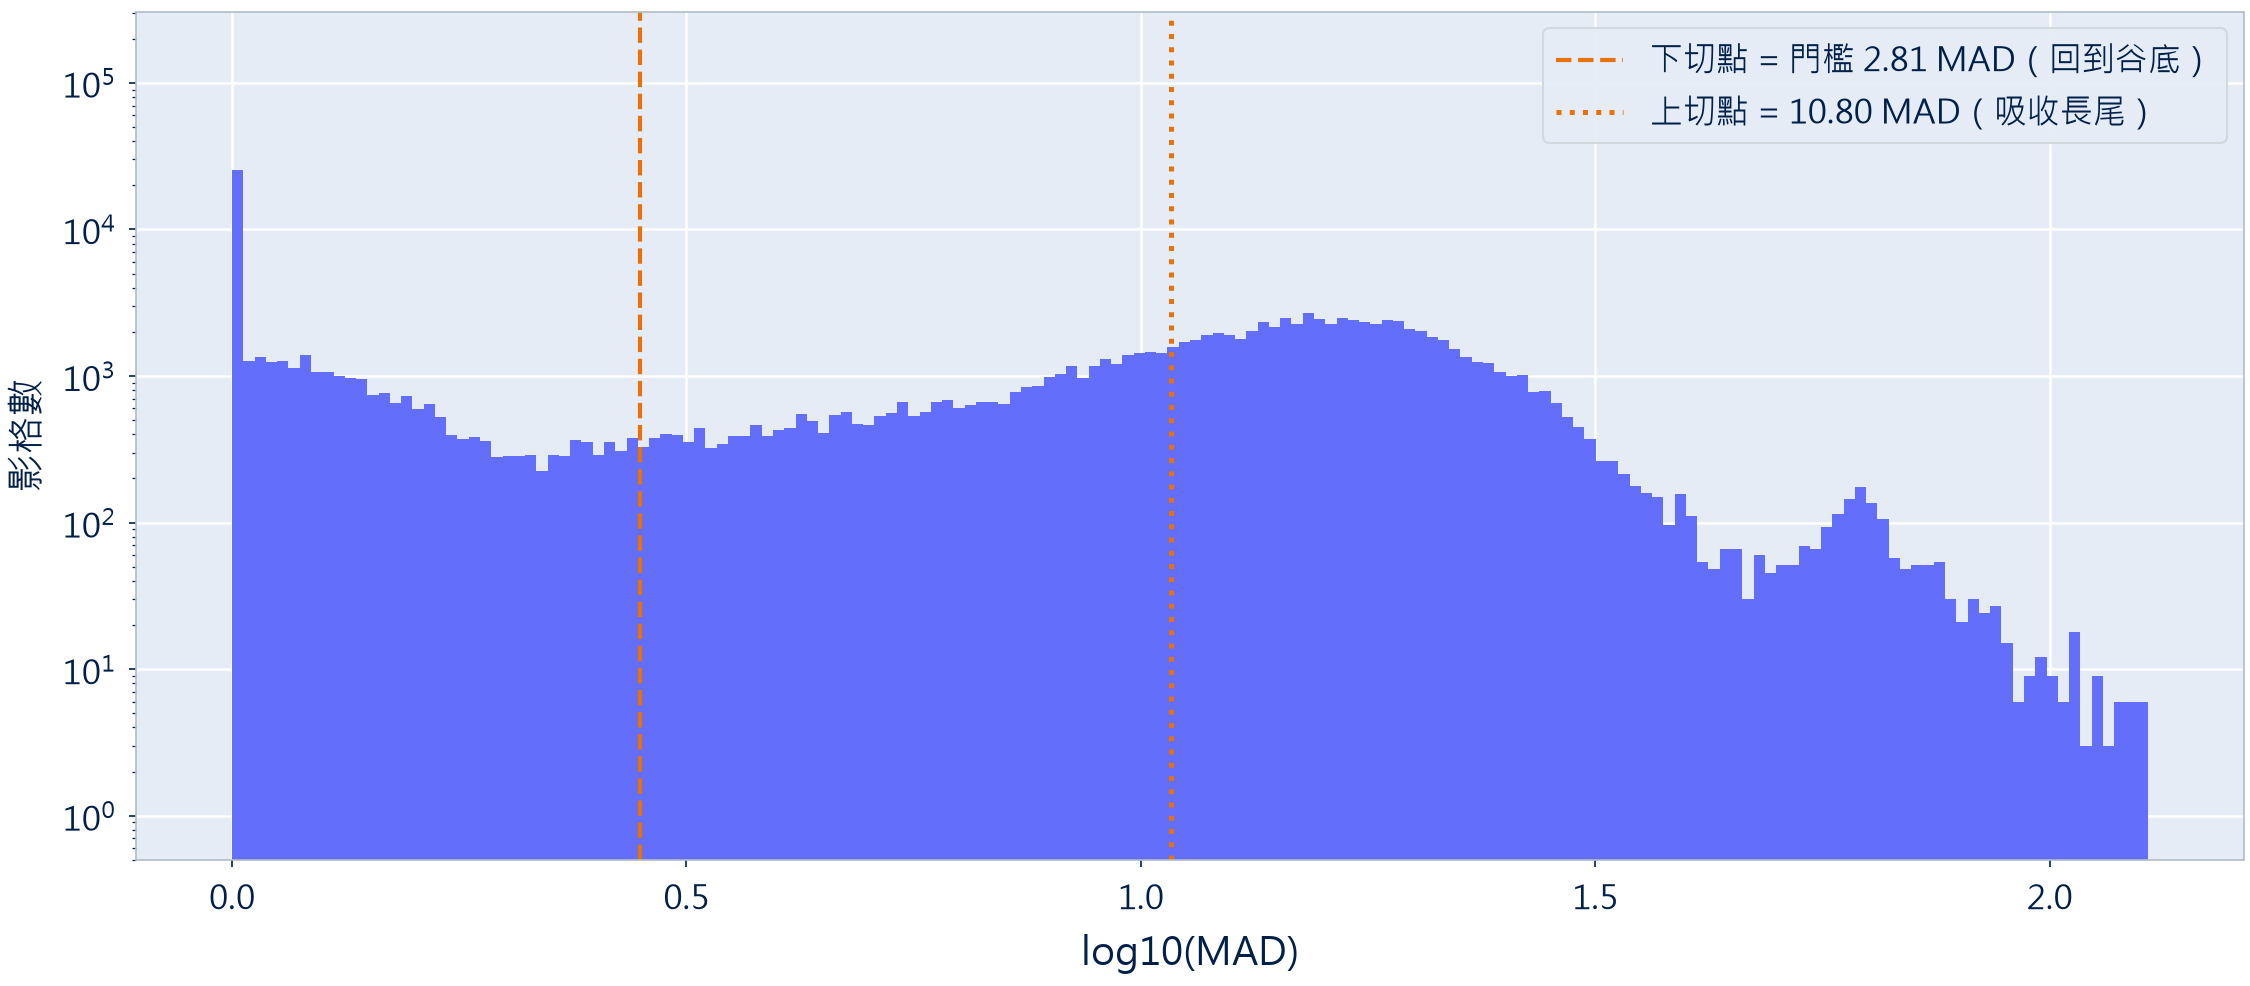
\includegraphics[width=\linewidth]{match_segmentation/otsu_3class.png}
  \caption{三類 Otsu 的兩個切點}
  \label{fig:otsu-3class}
\end{figure}

\subsubsection{跨片段一致性篩選}

將連續低 MAD 影格串接成片段，此時保留下來的片段中仍混有計分板、定格等靜止片段。關鍵觀察是，此時剩餘的固定機位比賽片段數量多，且全部來自同一個固定機位、彼此在畫面上高度相似。其他片段則各自不同，與任何片段都不像。因此可以透過片段之間相互比較，判斷一個片段是否屬於佔多數的固定機位比賽片段。

設共有 $N$ 個片段，片段 $i$ 取其中央兩張影格，各自縮放至 $128\times72$ 並展開為特徵向量 $v_i^{(1)}, v_i^{(2)}$。兩片段的差異 $d(i,j)$ 取四組跨影格 MAD 的平均，跨片段平均差異 $\bar{d}(i)$ 則是片段 $i$ 對其餘 $N-1$ 段的平均：
\begin{equation}
  d(i,j) = \frac{1}{4}\sum_{a=1}^{2}\sum_{b=1}^{2} \mathrm{MAD}\!\left(v_i^{(a)},\, v_j^{(b)}\right),
  \qquad
  \bar{d}(i) = \frac{1}{N-1} \sum_{j \neq i} d(i,\, j)
  \label{eq:cross-mad}
\end{equation}

\begin{figure}[H]
  \centering
  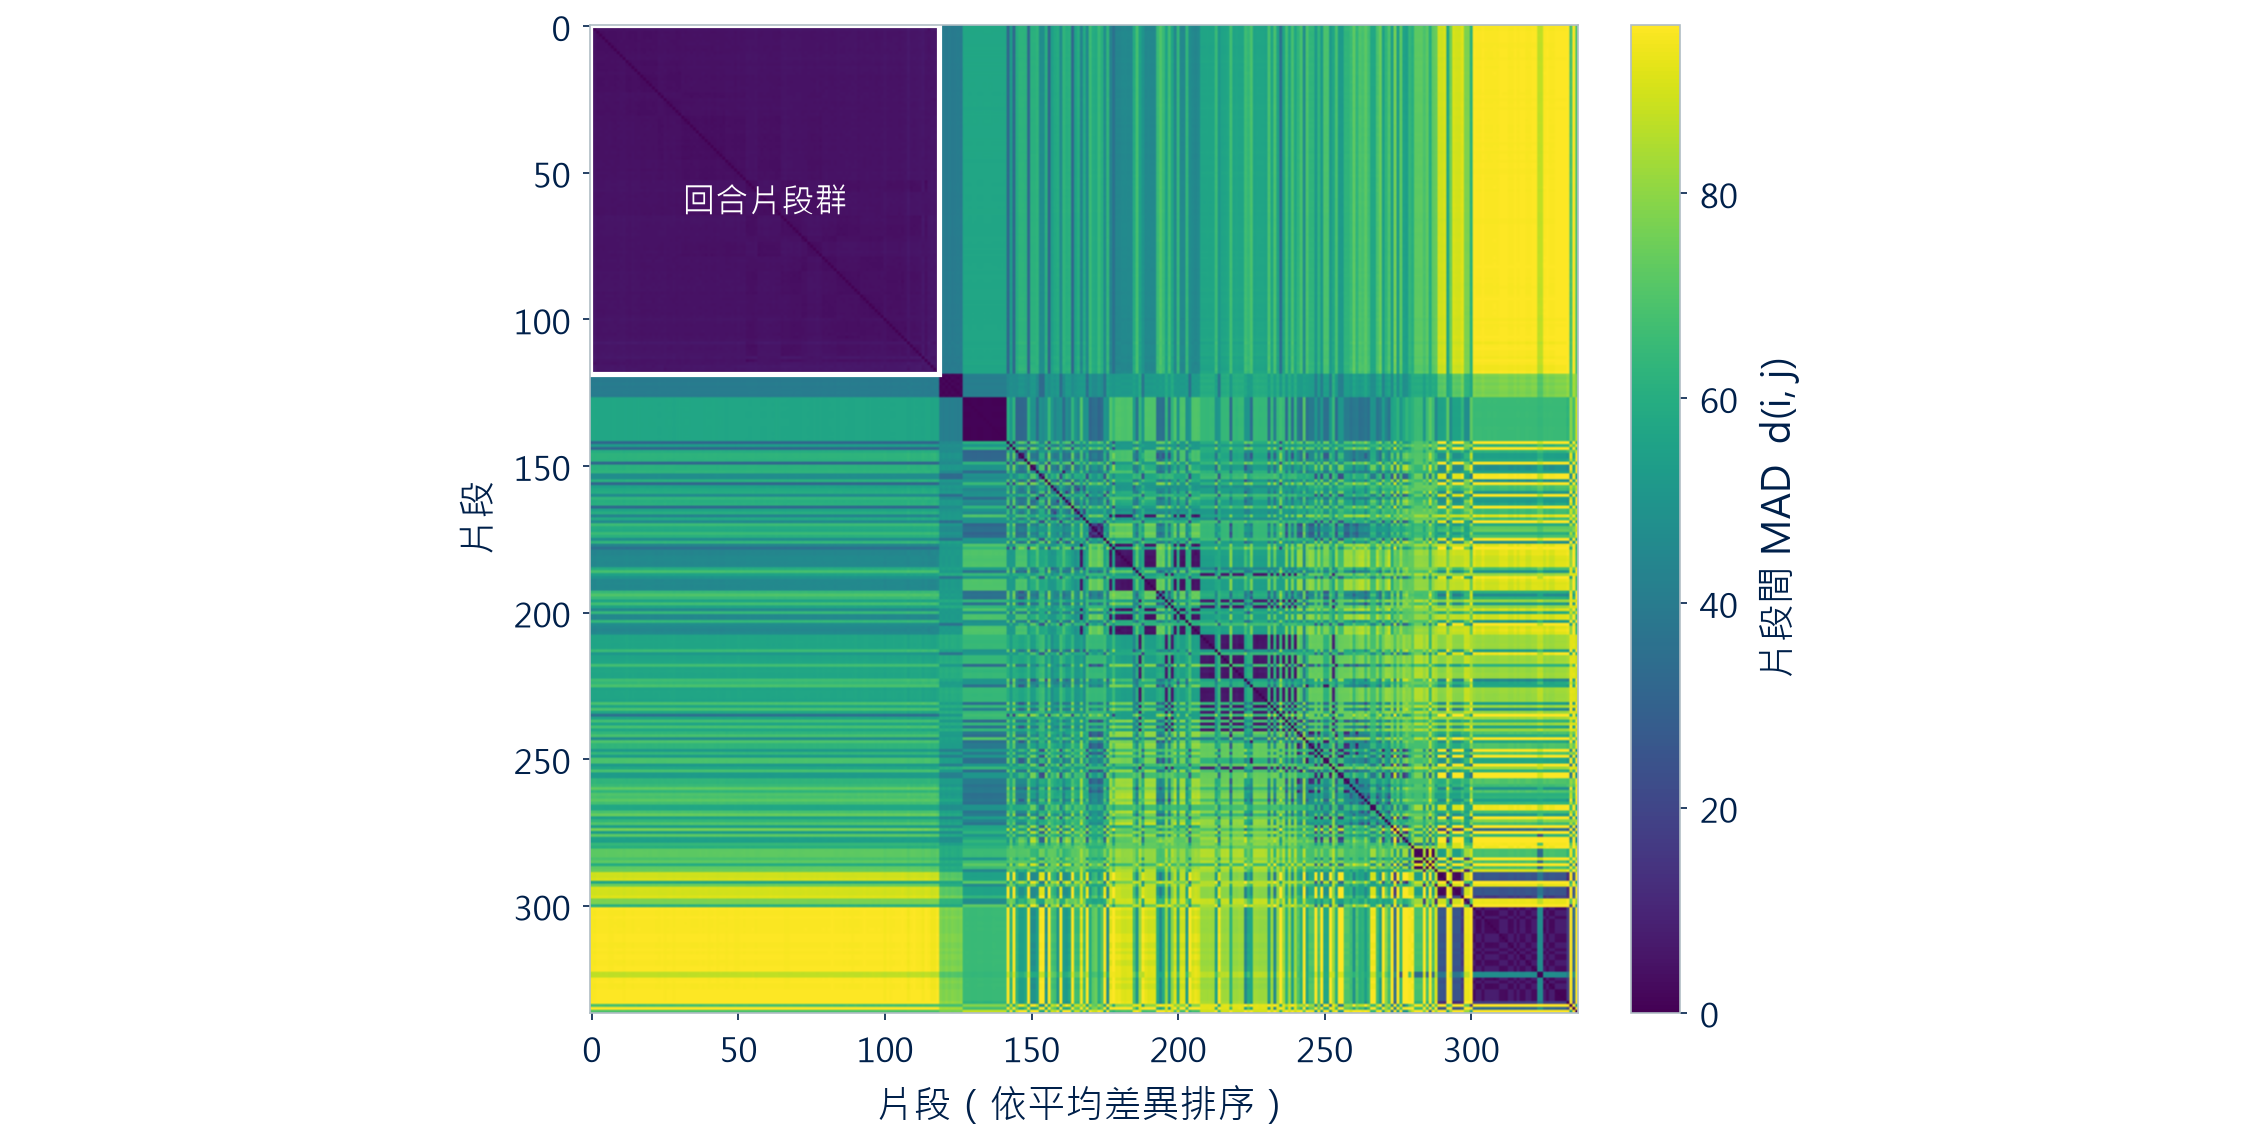
\includegraphics[width=\linewidth]{match_segmentation/cross_matrix.png}
  \caption{跨片段兩兩 MAD 矩陣（依平均差異排序）}
  \label{fig:cross-matrix}
\end{figure}

因為所有固定機位比賽片段高度相似，它的 $\bar{d}(i)$ 幾乎只由少數幾個非固定機位比賽片段貢獻，數值因而偏低。又因固定機位比賽片段彼此相像，算出的 $\bar{d}(i)$ 也幾乎相等，於是它們在直方圖最左側聚成一個緊密的群。其他片段畫面各異，$\bar{d}(i)$ 偏高且分散。\figref{fig:cross-matrix}將片段依 $\bar{d}(i)$ 排序，左上角的紫色密集區即這群固定機位比賽片段。

實測固定機位比賽片段間 $\bar{d}(i)$ 的極差在 5\% 以內，最小的非固定機位比賽片段比全體最小值大 13\%，門檻取全體最小值的 1.07 倍（\figref{fig:cross-avg}）。此門檻成立的前提是固定機位比賽片段屬於最緊密的群，若影片含大量彼此相似的畫面，會形成新的低 $\bar{d}(i)$ 群使門檻失效。

\begin{figure}[H]
  \centering
  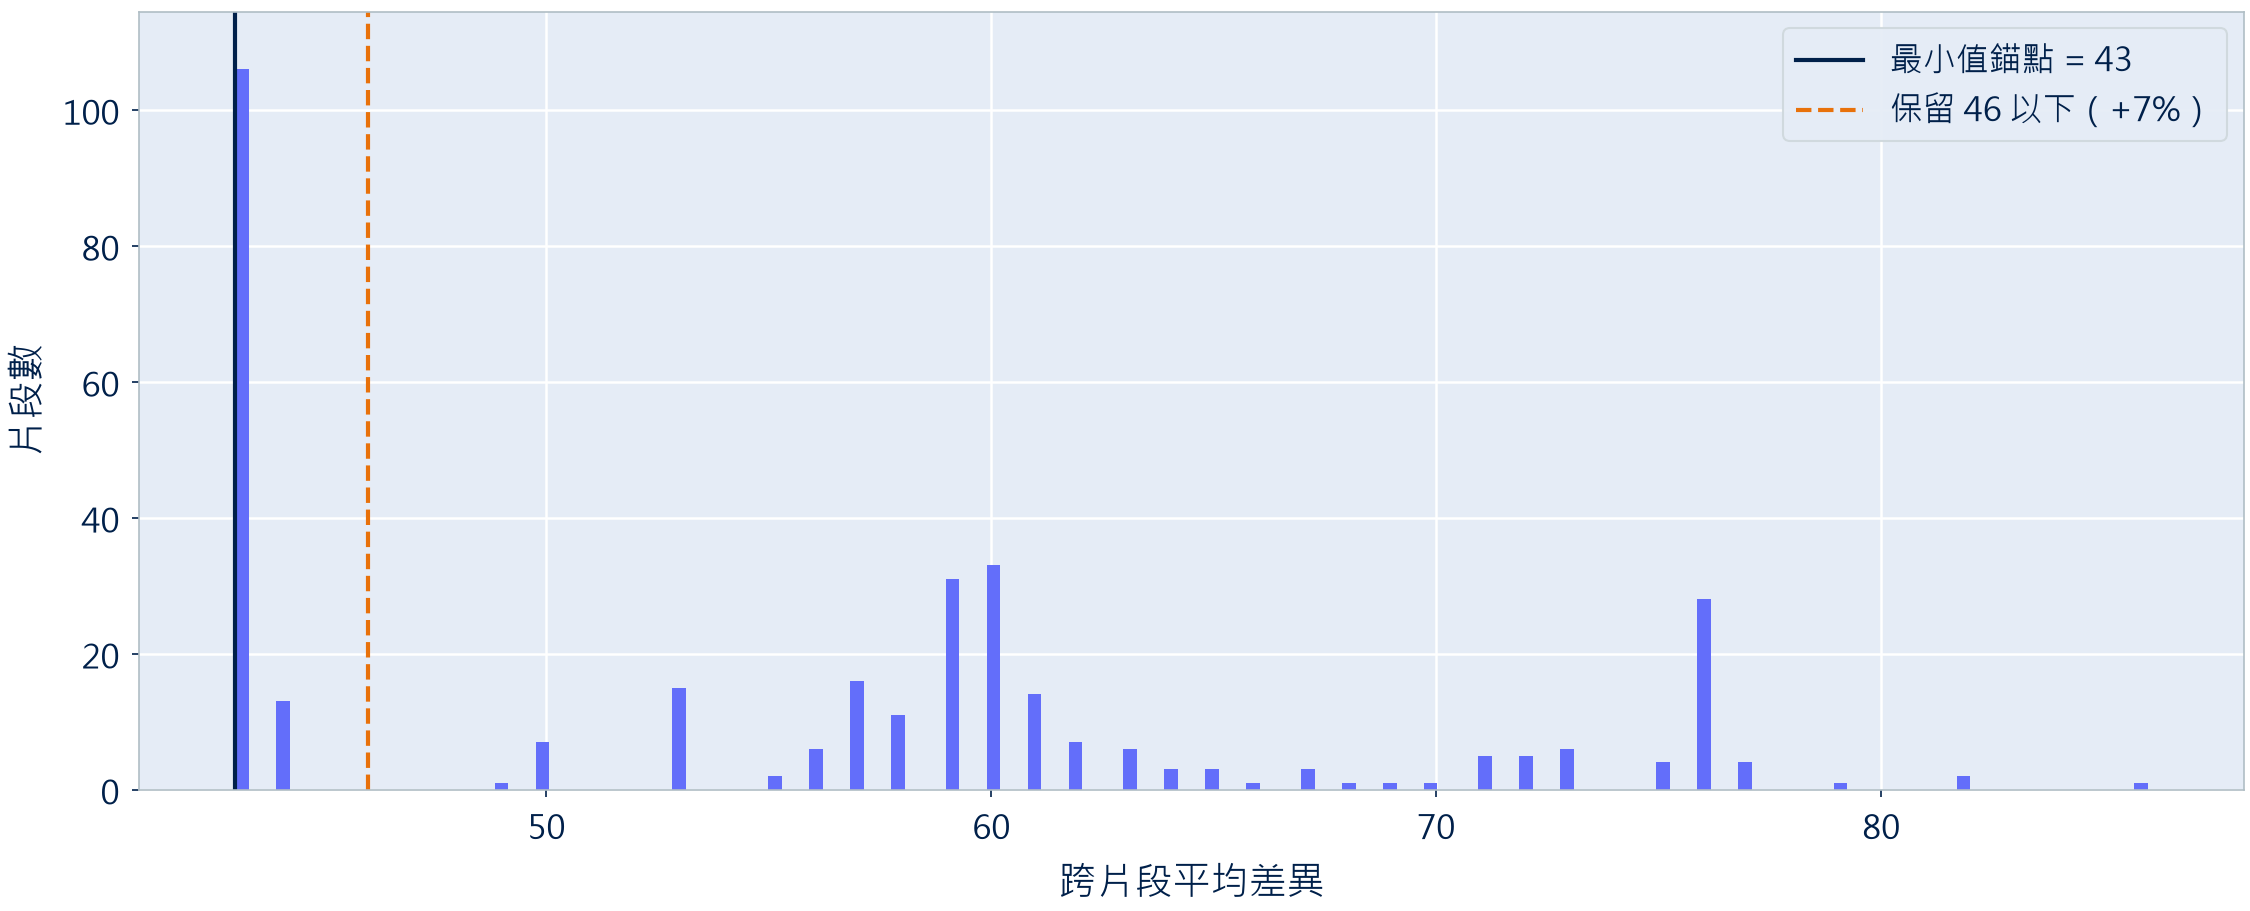
\includegraphics[width=\linewidth]{match_segmentation/cross_avg.png}
  \caption{跨片段平均差異的分佈與門檻}
  \label{fig:cross-avg}
\end{figure}

通過篩選的片段中偶爾仍殘留鷹眼判定、官方重播等電腦合成畫面，其構圖與固定機位比賽畫面接近。因此對剩餘片段再算一次跨片段平均差異，採較嚴格的門檻，捨棄超過中位數三倍者。

\subsubsection{邊界精修}

此階段把被少數高 MAD 影格（分數卡片動畫）切碎的片段接回。同時第一階段的跳幀取樣使邊界存在系統性偏差，需還原到影格層級。

\textbf{做兩次片段連接：}第一次只看距離，間距小於 5 張影格的相鄰片段直接接合。第二次針對 12 張影格以內的間隙逐影格重新掃描，僅當間隙內最大相鄰 MAD 低於 25（即不存在尖峰）時才接合。

\textbf{做邊界對齊：}在每個邊界附近逐影格計算相鄰 MAD，尋找同時滿足絕對值門檻與區域中位數倍率的尖峰，此尖峰對應剪接點，起點設為切入尖峰所在的影格，終點設為切出尖峰的前一張影格。

\begin{figure}[H]
  \centering
  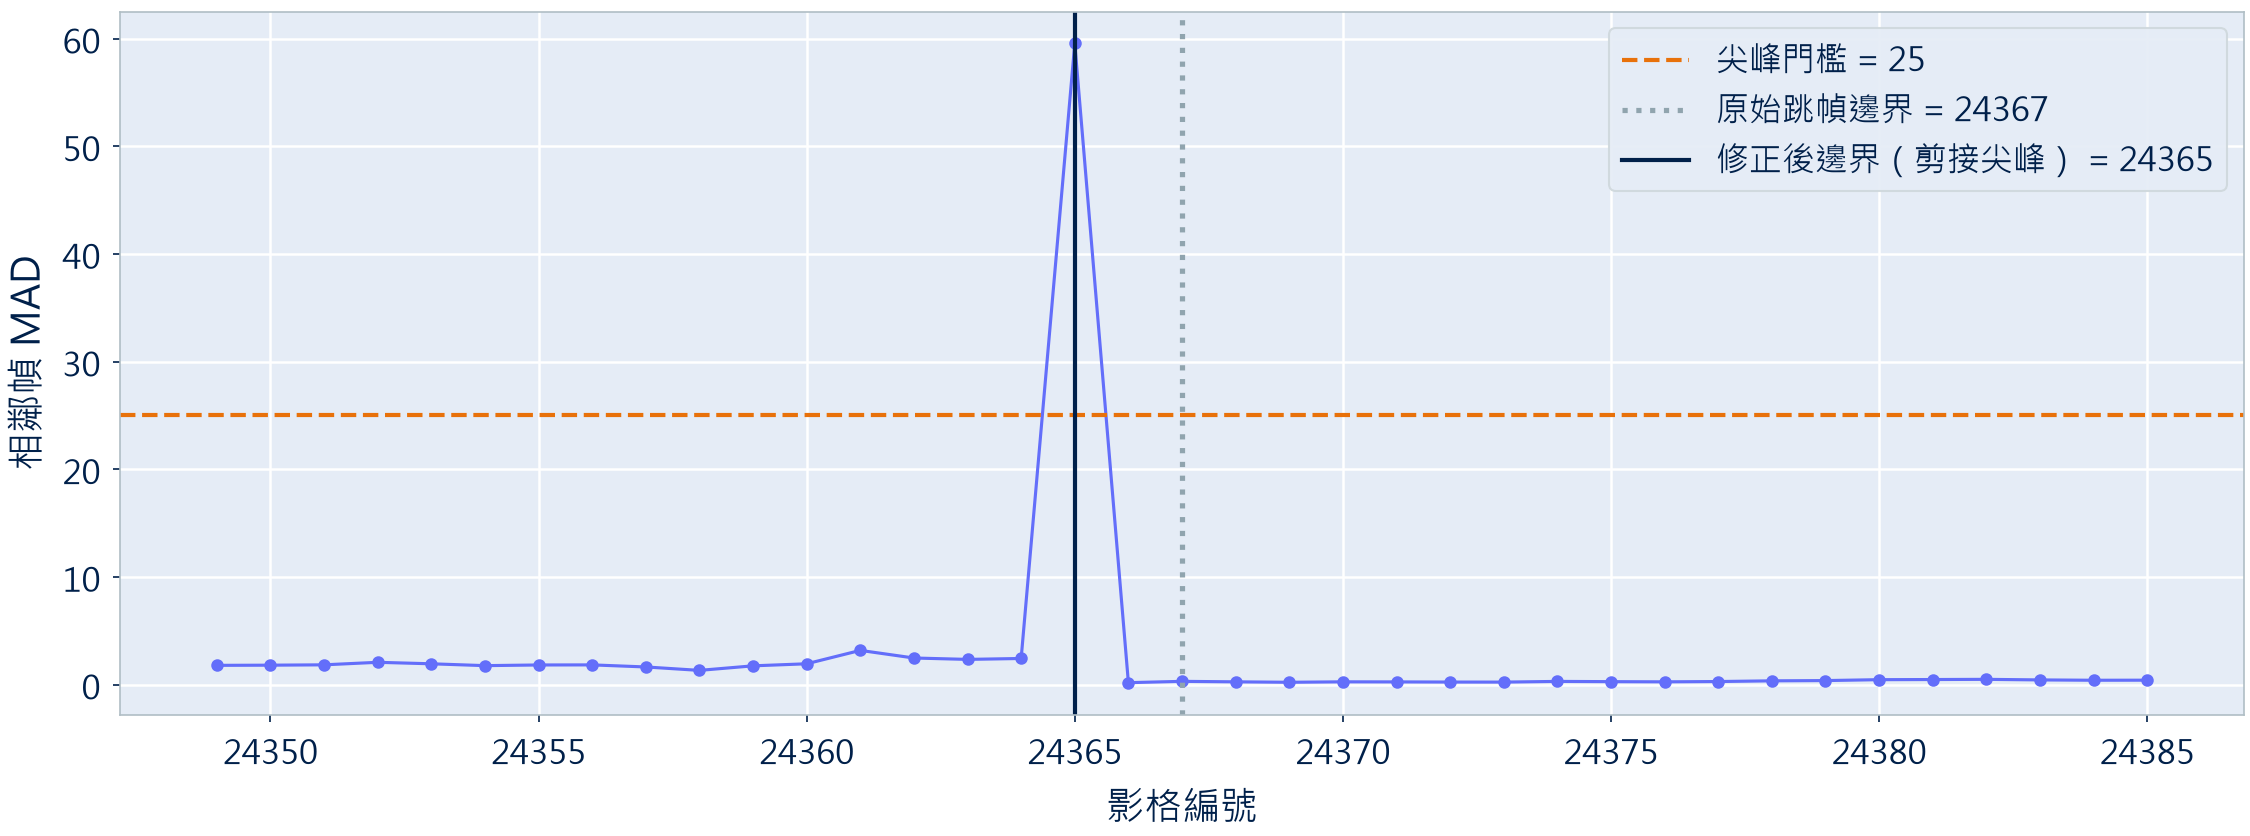
\includegraphics[width=\linewidth]{match_segmentation/cut_spike.png}
  \caption{邊界尖峰偵測與修正}
  \label{fig:cut-spike}
\end{figure}

\figref{fig:cut-spike}中灰色點線為原始跳幀取樣邊界，深藍實線為修正後的邊界，橘色虛線為尖峰門檻。

\subsection{比分辨識}
\label{sec:score-recognition}

\subsubsection{概述}

\textbf{問題與目標：}賽事影片分段模組切出的片段中，同一回合可能因中間插入重播、特寫而被切成數段，一個片段也可能因為沒有鏡頭切換而包含多個回合。本模組為每個片段讀出畫面上的計分板比分，判斷片段所屬的回合，該比分同時供下游精彩片段分析使用。

\textbf{設計重點：}讀計分板天生受三個困難制約：泛化性（各賽事的計分板設計、位置不固定，且須避開干擾文字）、可讀性（計分板小又模糊）、多局制（三局制計分板易讀錯局）。本模組不需訓練模型或逐賽事調參，以「把難題拆成模型擅長的小任務、再用程式補上模型不擅長的部分」為核心，有三點做法：

\begin{enumerate}
  \item \textbf{使用視覺語言模型（VLM）：}目前使用傳統 OCR 的開源專案都需要手動標記計分板的位置。VLM 直接理解畫面結構，依視覺上下文自行分辨比分。不用為每種計分板寫過濾規則或手動標記，提升跨賽事的泛化能力。
  \item \textbf{多幀合成：}利用逐像素合成，強化計分板、糊化背景和球員。在 overlay 只出現於三成影格時仍能完整還原。
  \item \textbf{提示詞設計：}轉錄取代挑選，令模型由左到右完整抄寫計分板上所有數字（模型擅長），把當前局比分的挑選（模型易錯）移到程式端，讓較便宜的模型也能快速、正確的完成任務。
\end{enumerate}

\textbf{處理流程總覽：}如\figref{fig:score-recognition-flow}。

\begin{figure}[H]
  \centering
  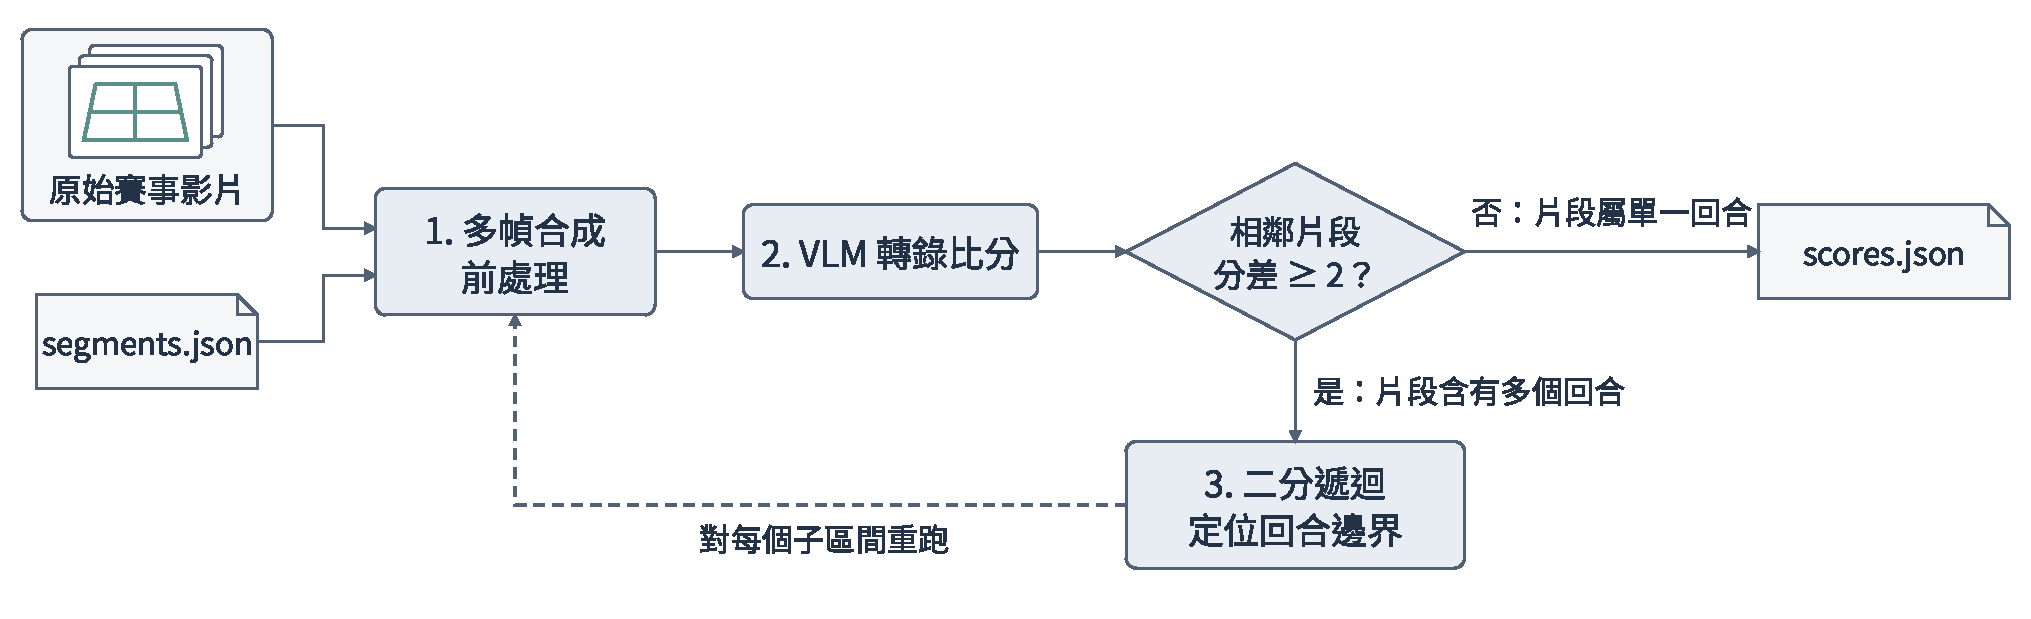
\includegraphics[scale=\flowscale]{score-recognition.pdf}
  \caption{比分辨識處理流程}
  \label{fig:score-recognition-flow}
\end{figure}

\subsubsection{多幀合成前處理}

本步驟為每個片段產生一張合成圖，讓 VLM 讀一張圖就拿到比分。轉播的計分板 overlay 只在片段的部分影格出現，若逐張送 VLM 去找，每個片段都得呼叫多次。一個片段通常同屬一回合，比分不變、計分板靜態，因此把片段取樣的多張影格逐像素合成，間歇出現的計分板被疊加強化、穩定呈現在合成圖上，一個片段只需一次 API 呼叫。不斷移動的球員與觀眾被平均糊化，順帶為 VLM 濾去干擾。

合成採 \texttt{dominant\_cluster}（主群集平均）：對每個像素的亮度值分箱，只平均落入最多值的那一箱。overlay 出現時亮度幾乎固定，會全擠進同一箱。背景每幀不同而分散各箱。因此最密集的一簇即為計分板（\figref{fig:overlay-recovery}）。這個方法不預設目標信號在時間上佔多數，即使轉播 overlay 只間歇出現仍能保留。

\begin{figure}[H]
  \centering
  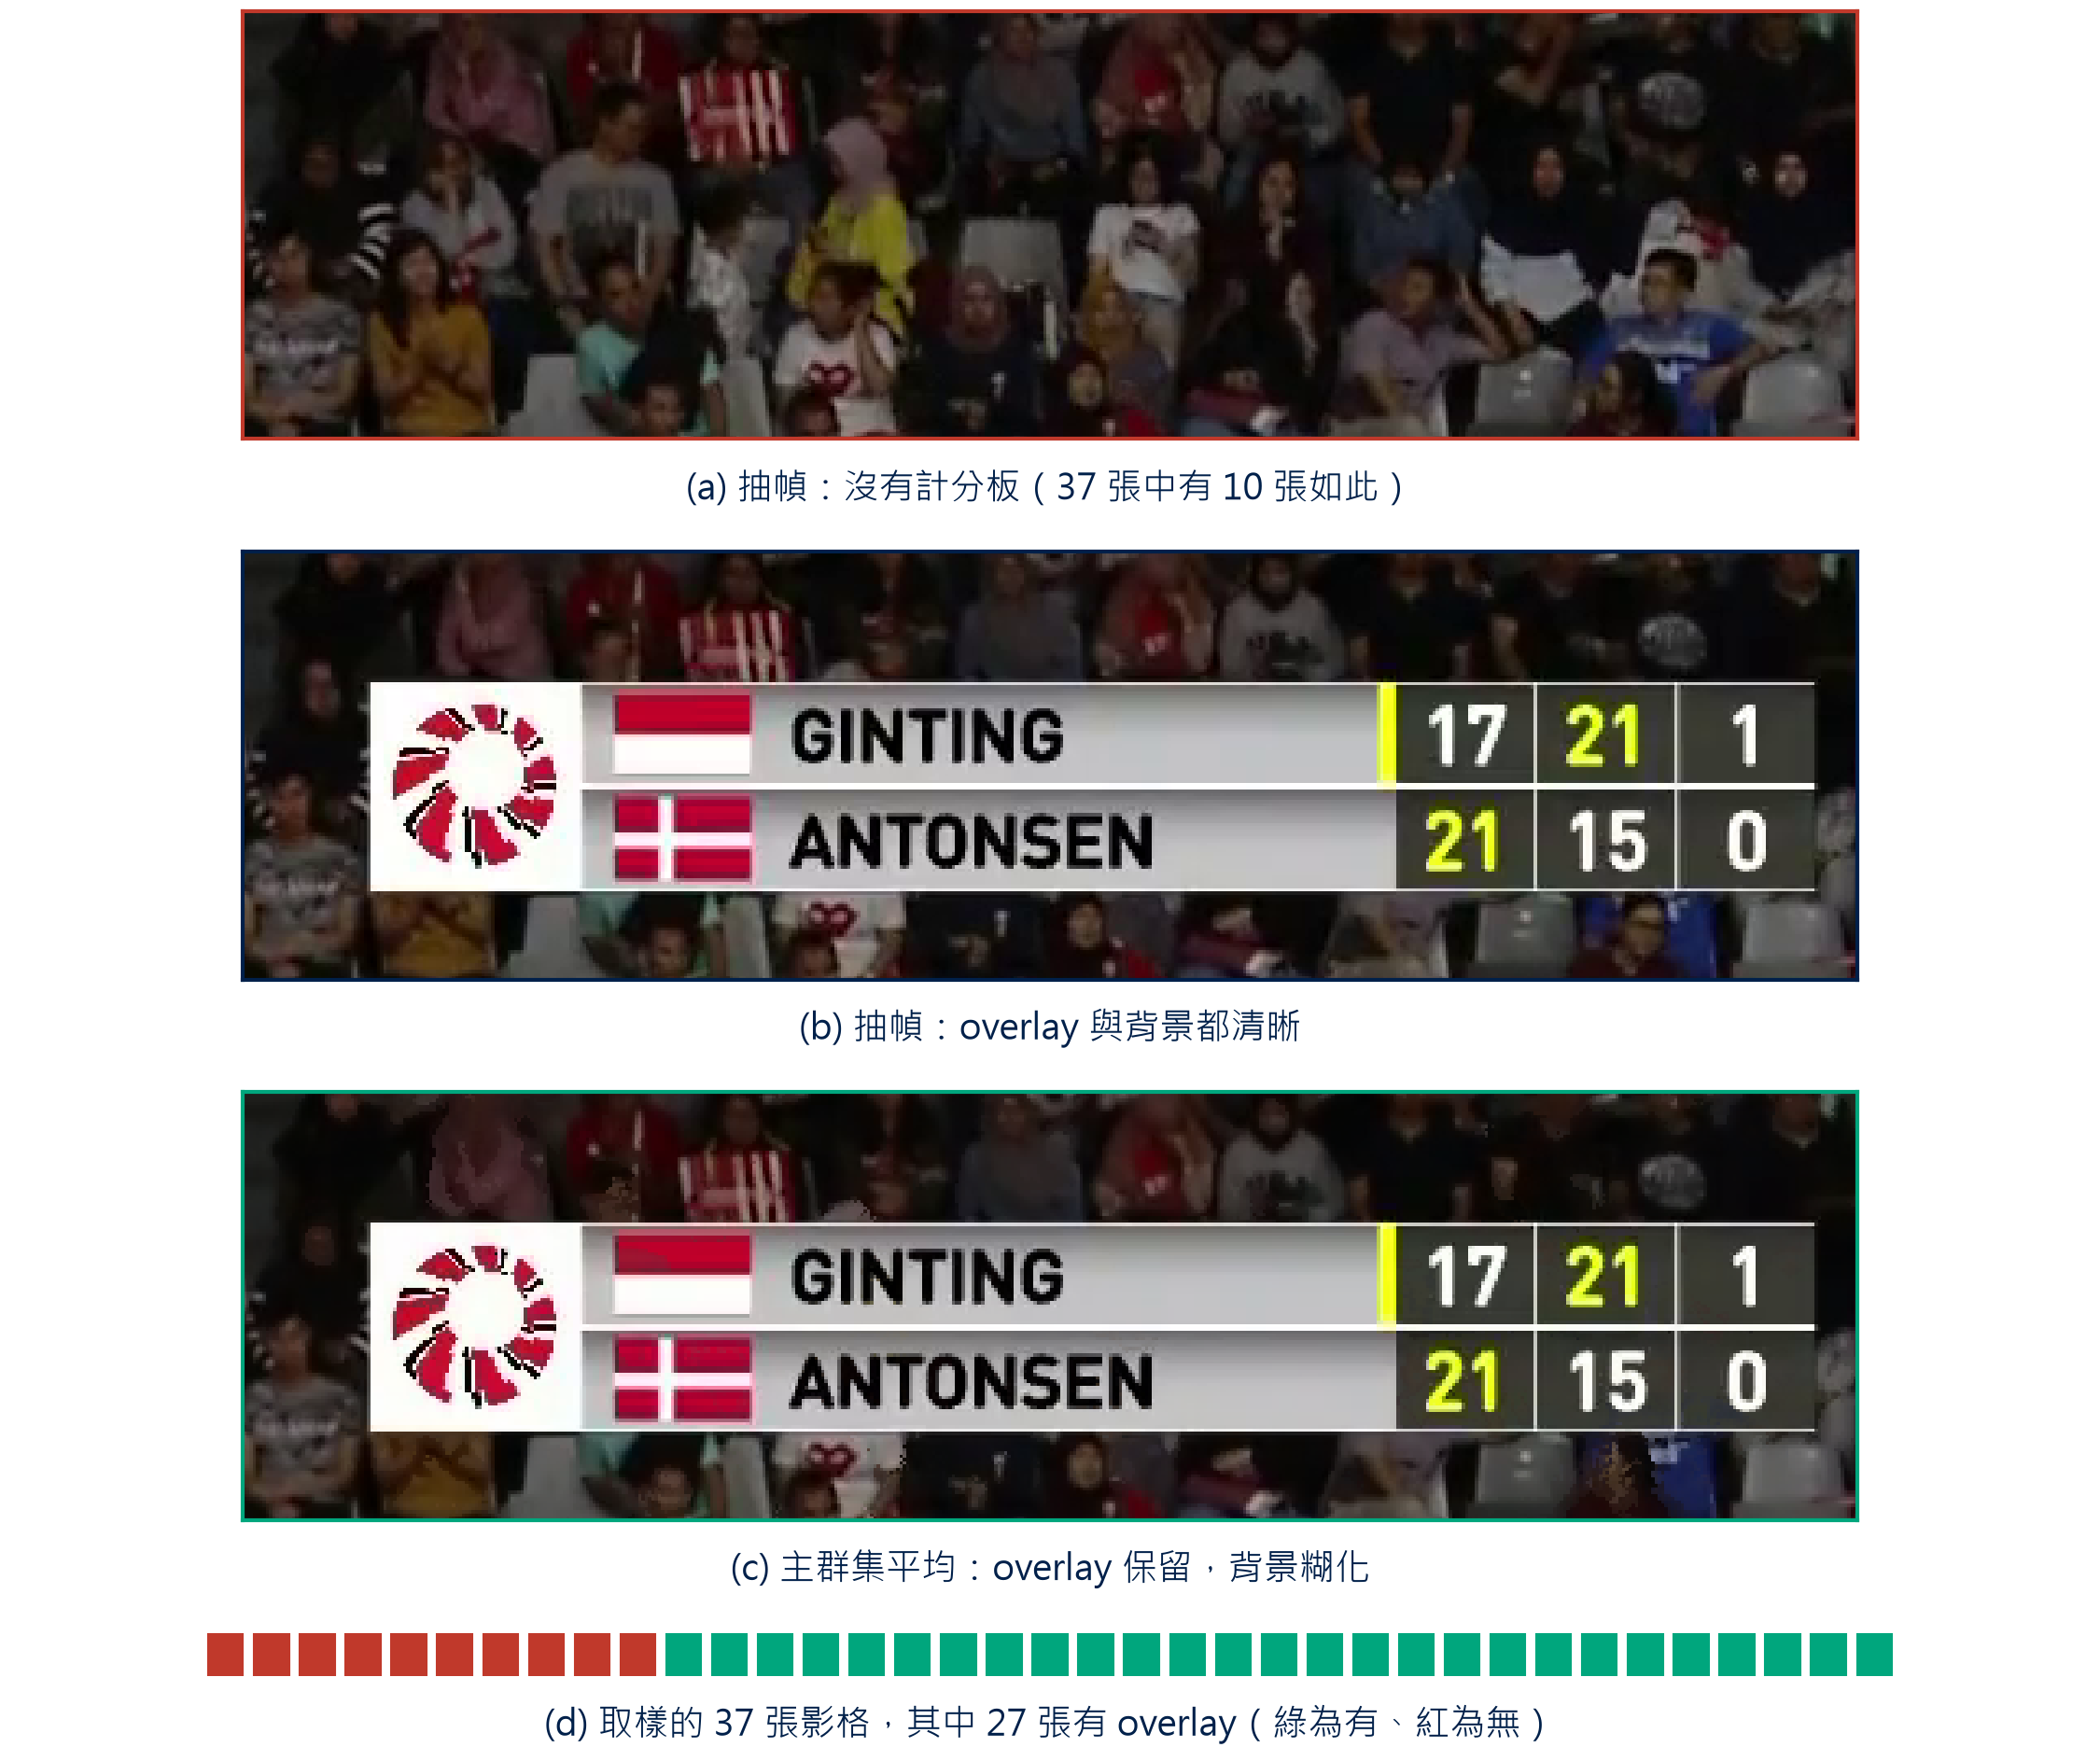
\includegraphics[width=\linewidth]{score_recognition/overlay_recovery.png}
  \caption{overlay 只出現在部分影格時，主群集平均的還原結果}
  \label{fig:overlay-recovery}
\end{figure}

\subsubsection{VLM 轉錄比分}

本步驟從合成圖讀出雙方當前比分。多局制計分板每隊並列多局數字，要模型直接判斷「哪個是當前局」容易錯，完整抄寫數字對模型來說不需要推理，比較簡單。因此只要求模型逐隊由左到右抄下所有數字，挑選交給程式，固定取每隊陣列最右一個為當前比分，從根源消除模型讀錯局的可能（\figref{fig:transcription-pick}）。

實作上使用 Gemini 2.5 Flash，將 temperature 設為 0，並且關閉 thinking，減少結果變化的同時避免模型進行不必要的推理，多餘的推理浪費 token、時間又容易出錯。

\begin{figure}[H]
  \centering
  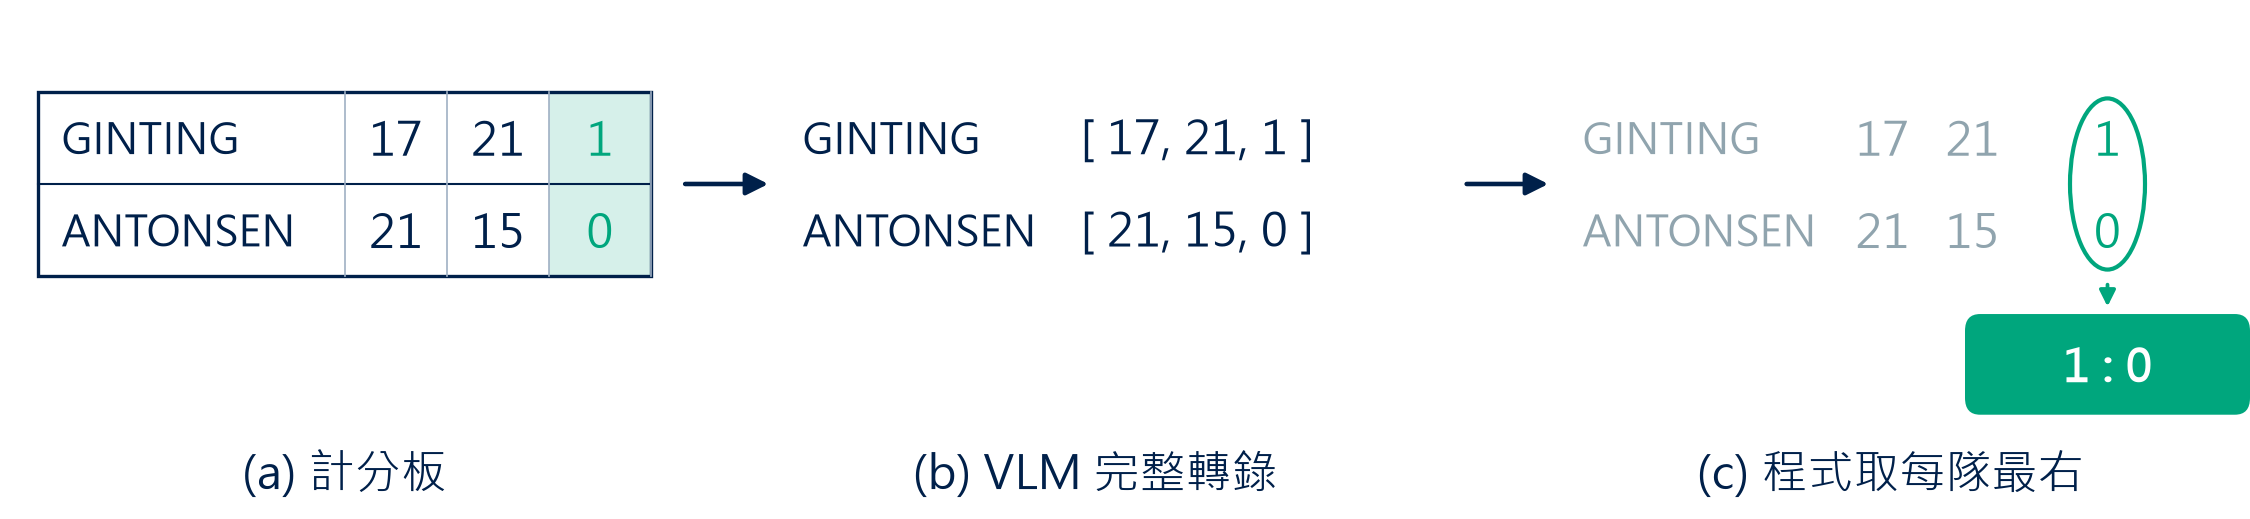
\includegraphics[width=\linewidth]{score_recognition/transcription_pick.png}
  \caption{轉錄取代挑選，VLM 完整抄寫每隊數字，程式取最右一個為當前比分}
  \label{fig:transcription-pick}
\end{figure}

\subsubsection{還原被合併的回合}

分段以鏡頭切換為訊號，兩回合間若沒有切換就會被併進同一片段，此時計分板在片段中途變動，單張合成只讀得到其中一個回合。本步驟負責找出並拆開這類片段。

判斷靠比分本身，正常一回合雙方總分只加一分，因此若某片段雙方比分總和一次增加兩分以上，就代表中間有回合沒被單獨切出，標記為合併片段。

標記後以二分搜尋定出回合交界，在候選區間中點重新合成、辨識比分，與兩端比較，往比分仍有跳變的一側收斂，逼近比分改變的影格。由於一個片段可能併入不只兩回合，每定出一個切點就對兩側子區間各自遞迴、繼續二分，直到每個子區間都只差一回合。

\section{場景與人體理解}
\label{sec:scene-understanding}

\subsection{場地偵測}
\label{sec:court-detection}

\subsubsection{概述}

\textbf{問題與目標：}後續所有球員與球體分析需要以球場座標來解讀位置與距離。本模組從固定俯拍的轉播畫面中定出球場，建立影像平面與球場平面投影的座標基準，供後續步驟使用。

\textbf{設計重點：}本模組不需訓練模型、不需標註，核心是把球場偵測化約為「在畫面中找四個外角」的問題，球場是平面、尺寸由競賽規則規定，定出四角即可解出單應性，其餘 12 條線與 16 個交點全由它投影得出。本模組的初始版本參考了一份以 OpenCV 實作的開源羽球場地偵測程式~\cite{badmintoncv}，現行版本在其基礎上重新設計，將顏色寫死的處理改為顏色無關的表面分割，並以消失點過濾與網格枚舉取代原本 $O(n^4)$ 的四邊線窮舉。在此基礎上有三點做法：

\begin{enumerate}
  \item \textbf{零先驗的顏色自適應：}球場顏色因場館而異，系統不預設任何色彩範圍，參考色與門檻全從畫面即時估計。相較多數開源方案需固定顏色範圍或手動標記，本法無需逐場調參。
  \item \textbf{多來源並聯、統一吻合度評分裁決：}不押注單一路徑，兩種遮罩、三種外角來源並行推導，最後由同一個「場線像素吻合度」的評分選出最佳者。遮罩斷裂這類錯誤不可逆，並聯確保唯一的路不會走死。
  \item \textbf{以最可靠的內部線反推最不可靠的外角：}球場外緣線透視壓縮最重、最常被遮斷，最難完整偵測。網格枚舉改由遮擋少的內部發球線與中線一起投票決定四角，把證據取用的方向倒轉過來。
\end{enumerate}

在 9 場未參與開發的比賽上，角點定位誤差中位數為 2.79 像素（見\secref{sec:exp-court}）。

\textbf{處理流程總覽：}如\figref{fig:court-detection-flow}。

\begin{figure}[H]
  \centering
  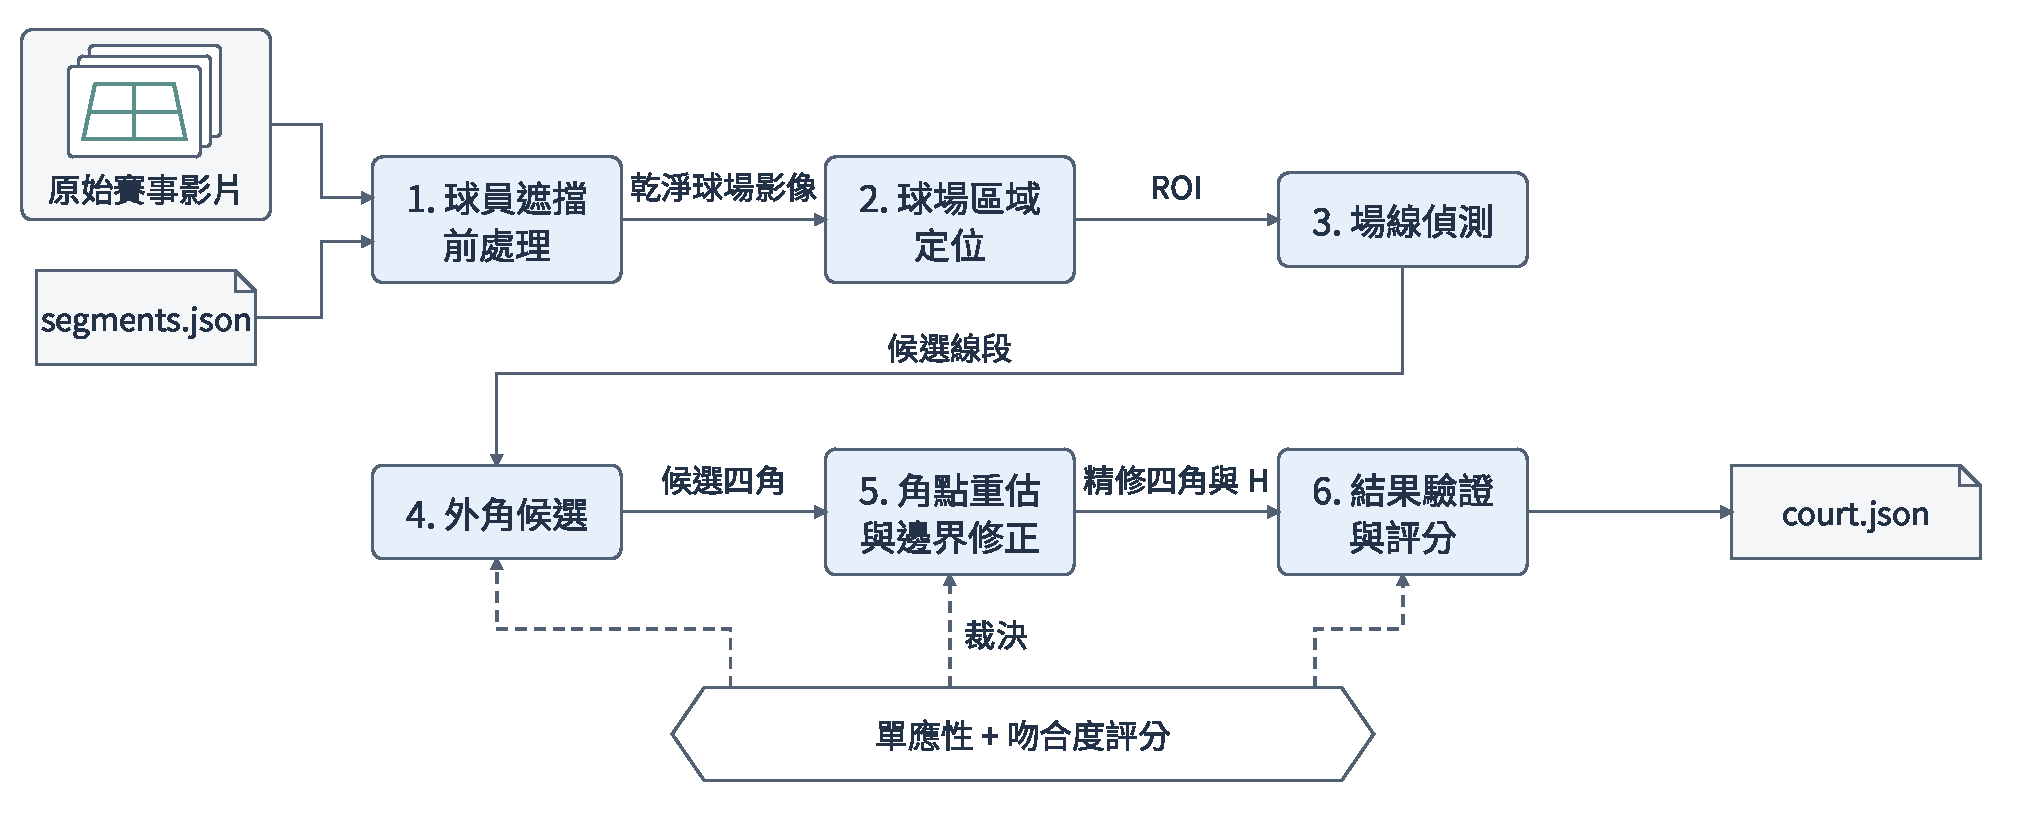
\includegraphics[scale=\flowscale]{court-detection.pdf}
  \caption{場地偵測處理流程}
  \label{fig:court-detection-flow}
\end{figure}

\subsubsection{球員遮擋前處理}

後續定位球場的主要訊號是顏色與場線，但轉播畫面中球員持續移動遮住場線與色塊，單張影格會使線條斷裂。本步驟要產生一張不含球員與短時雜訊的乾淨球場影像。機位固定時，球場在每張影格的同一座標都呈現相同顏色，唯有球員經過的少數影格例外，故對每個座標取多影格像素值的中位數，佔多數的球場顏色留下、屬於少數的球員與雜訊被濾除（\figref{fig:composite-median}）：
\begin{equation}
  M(x,y) = \mathrm{median}\{I_1(x,y),\dots,I_K(x,y)\}
\end{equation}

\begin{figure}[H]
  \centering
  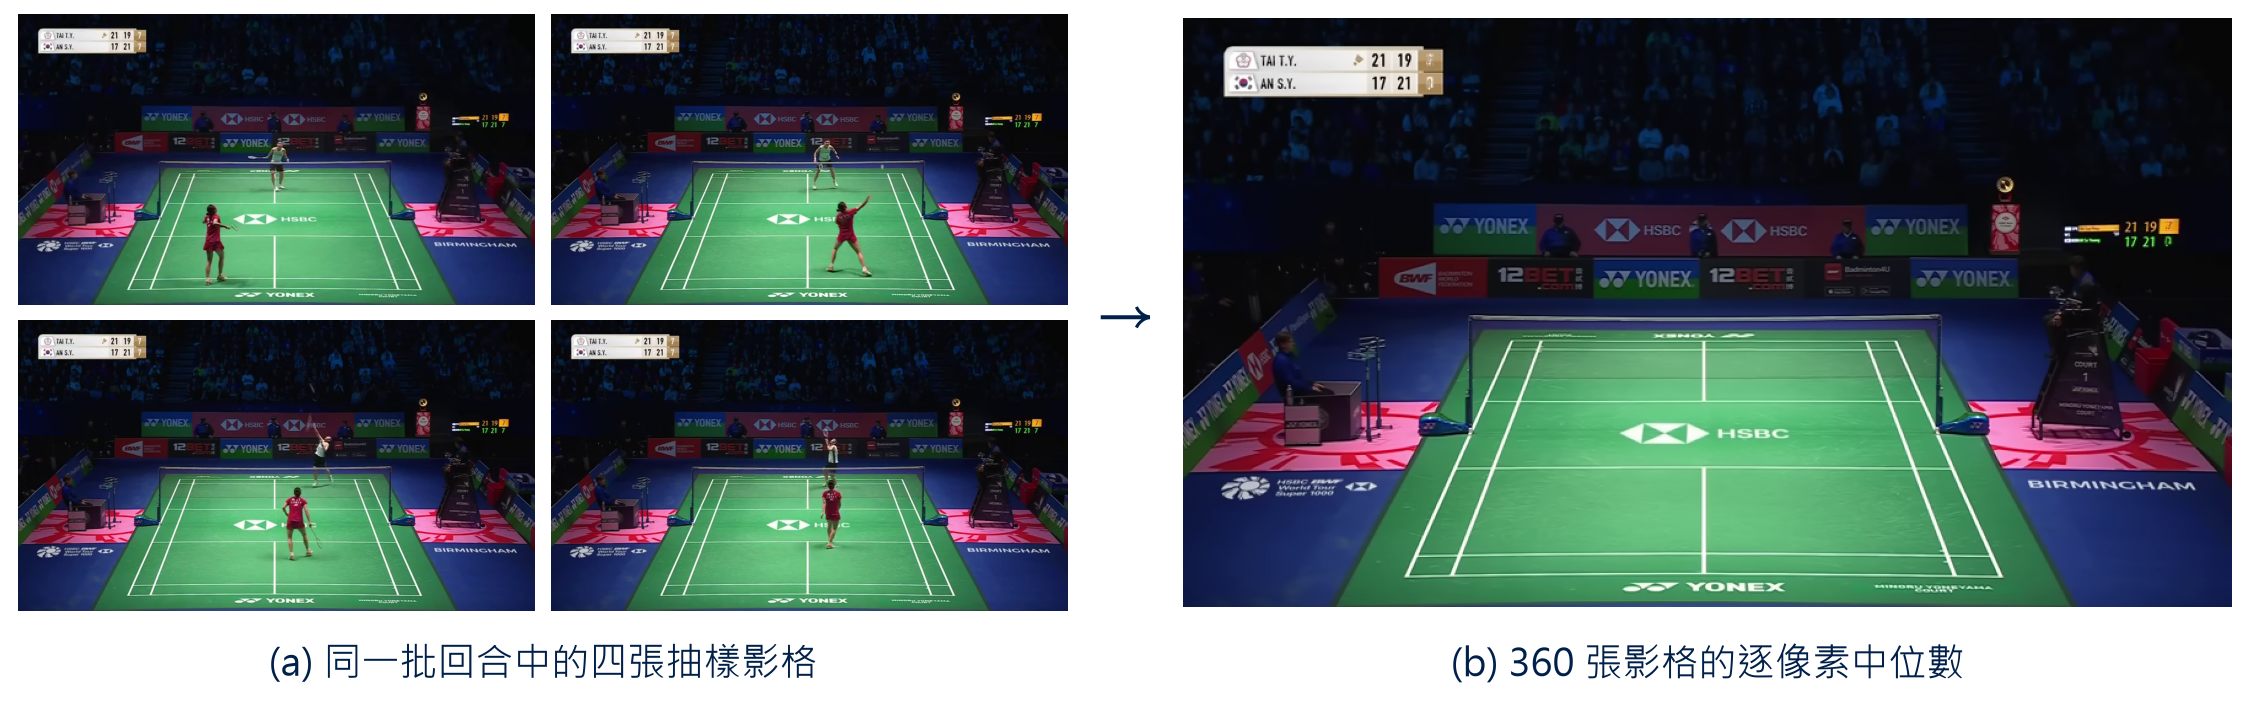
\includegraphics[width=\linewidth]{court_detection/composite_median.png}
  \caption{四張取樣影格與合成圖}
  \label{fig:composite-median}
\end{figure}

\subsubsection{球場區域定位}

本步驟要圈出球場在畫面中的大概範圍，好把範圍外的線段擋在後續場線偵測之外。實測對整張畫面掃描會得到近 200 條線段，真正屬於球場的只有 12 條（\figref{fig:mask-scope}）。

\begin{figure}[H]
  \centering
  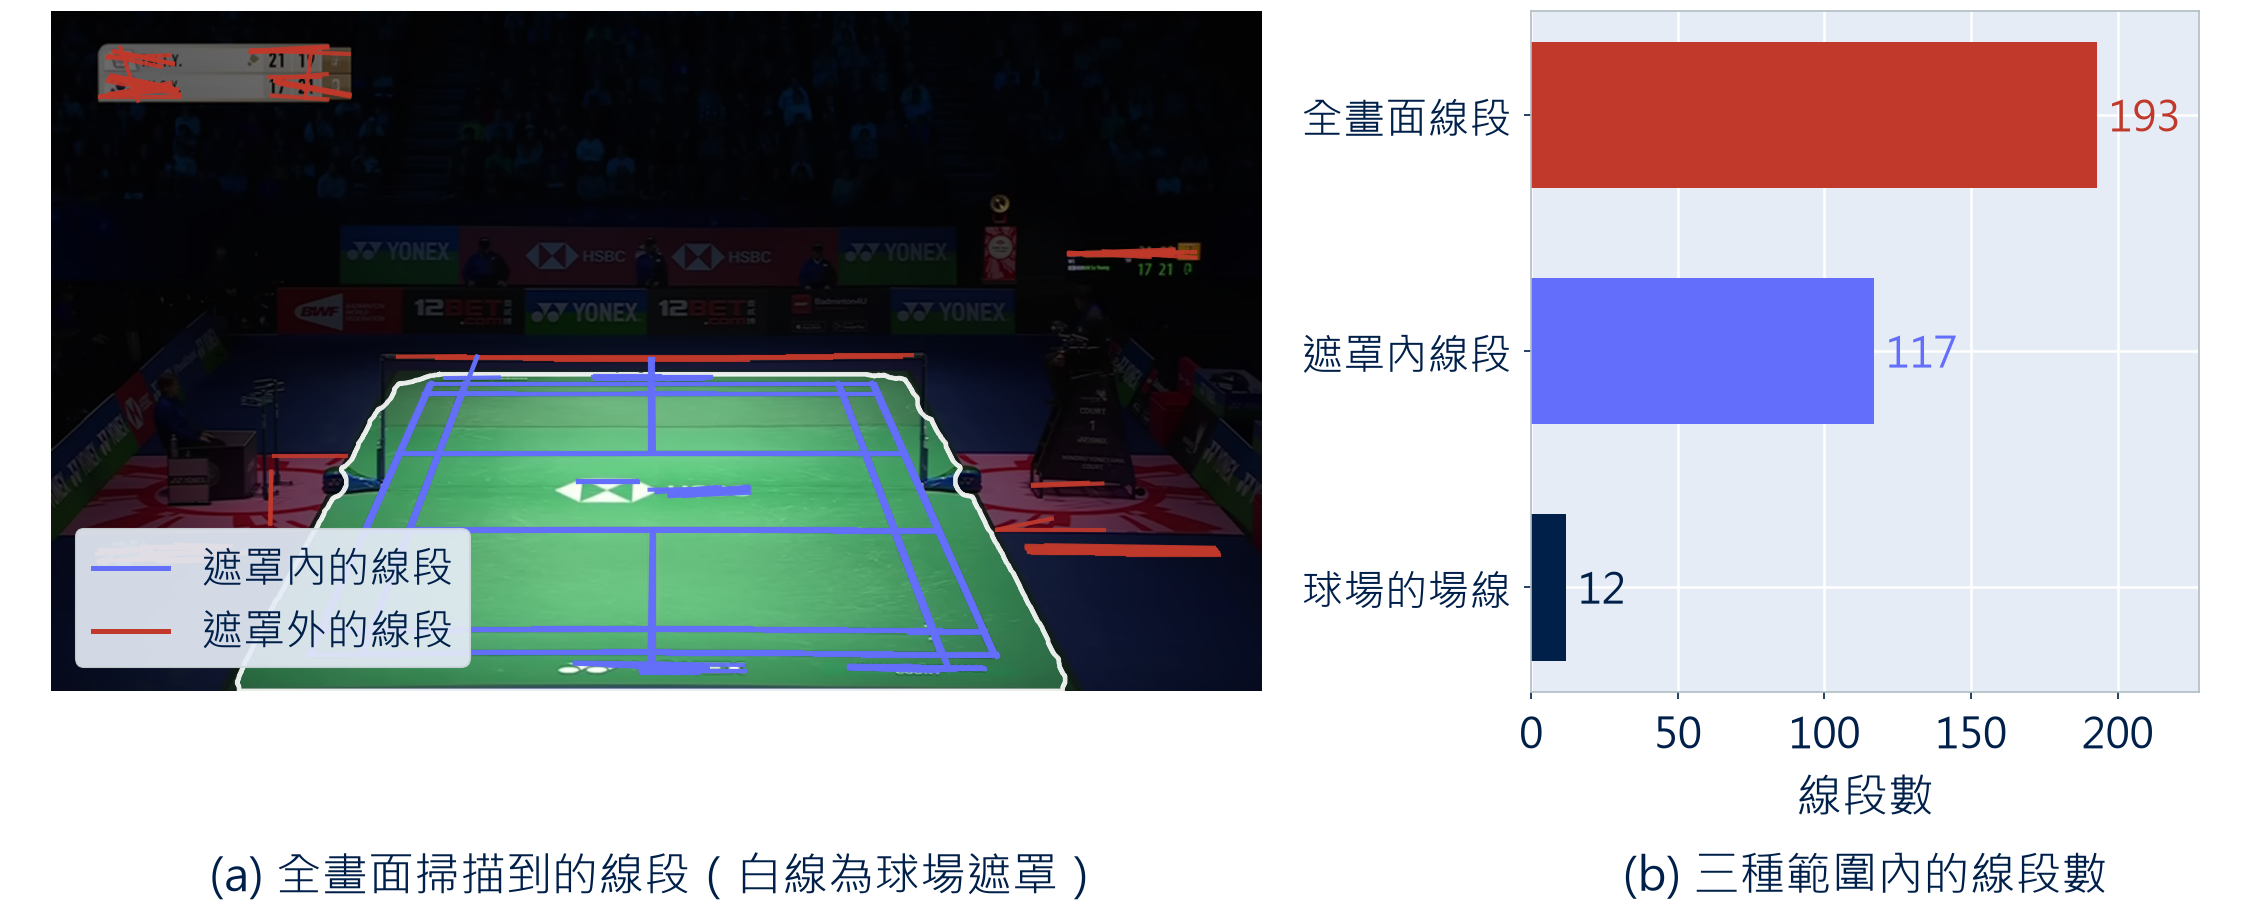
\includegraphics[width=\linewidth]{court_detection/mask_scope.png}
  \caption{全畫面掃描到的線段，與落在球場遮罩內的部分}
  \label{fig:mask-scope}
\end{figure}

分離球場與周邊地板的明顯特徵是顏色，但球場顏色本身未知。做法是在畫面中央偏下取一塊由機位假設保證落在場內的區域 $S$，取其像素在 Lab 色度（a、b）通道的中位數作為球場參考色 $\mathbf{c}$，任一像素的色度與 $\mathbf{c}$ 的距離小於門檻 $\tau_c$ 即判為球場：
\begin{gather}
  \mathbf{c} = \big(\mathrm{median}_{S}\,a,\ \mathrm{median}_{S}\,b\big), \qquad \tau_c = \max\!\Big(18,\ 3 \cdot \tfrac{\sigma_a + \sigma_b}{2}\Big) \\
  C(x,y) = \big[\,\lVert\,(a(x,y),\,b(x,y)) - \mathbf{c}\,\rVert < \tau_c\,\big]
\end{gather}
其中 $\sigma_a,\sigma_b$ 為 $S$ 在兩色度通道的標準差。捨棄亮度通道使光照與陰影不進入判斷。用中位數以避免取樣區塊內的像素影響門檻。門檻取 $3\sigma$ 使其隨取樣塊自身的顏色離散程度放寬，下限 18 則用以容忍過於平滑的場地（\figref{fig:lab-chroma}）。

\begin{figure}[H]
  \centering
  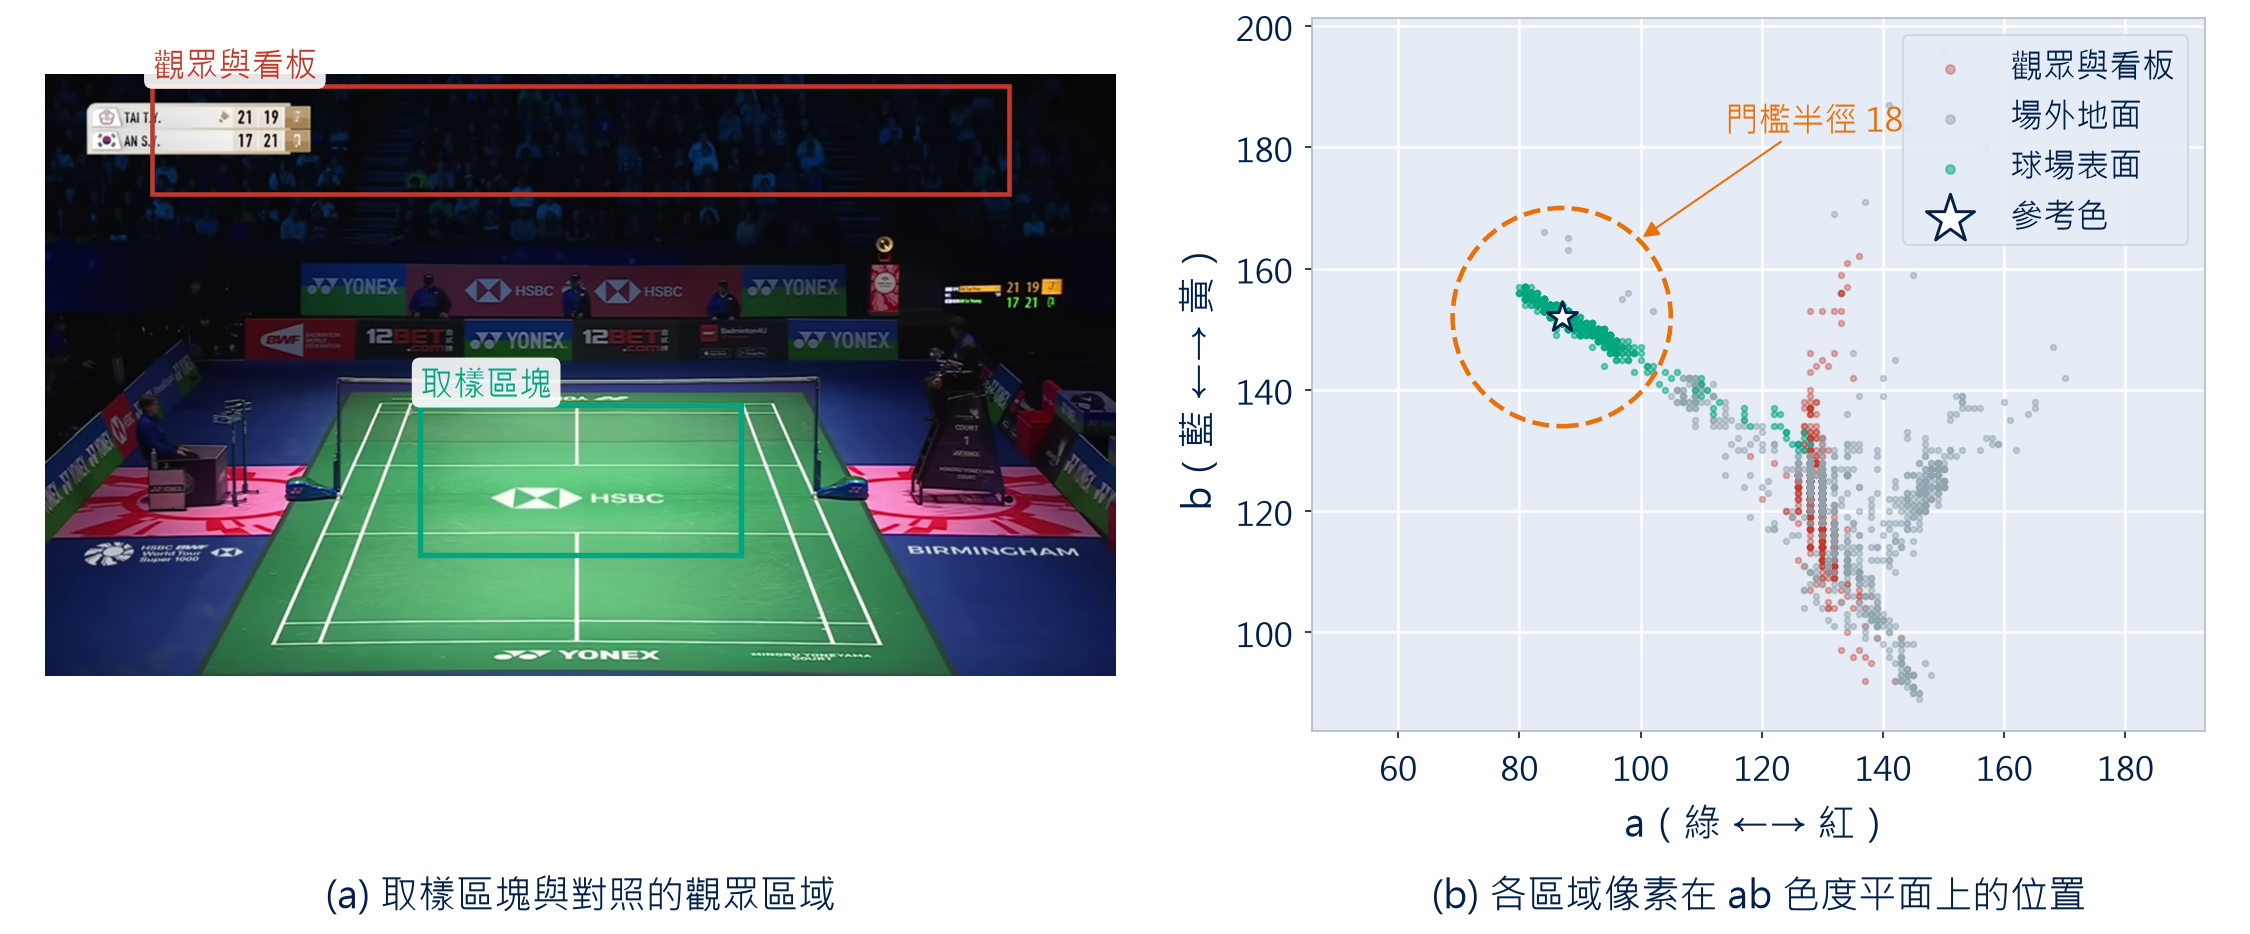
\includegraphics[width=\linewidth]{court_detection/lab_chroma.png}
  \caption{取樣區塊、參考色與門檻的判定}
  \label{fig:lab-chroma}
\end{figure}

上述門檻得到的是逐像素獨立的判斷，還不是一塊完整區域。白色場線把場地切成數塊，雜訊與反光留下零星破洞。模組以形態學運算補洞去雜點、取面積最大的連通區域、再自畫面左上角向內填充背景，把內部空洞併回球場（\figref{fig:morphology}）。

\begin{figure}[H]
  \centering
  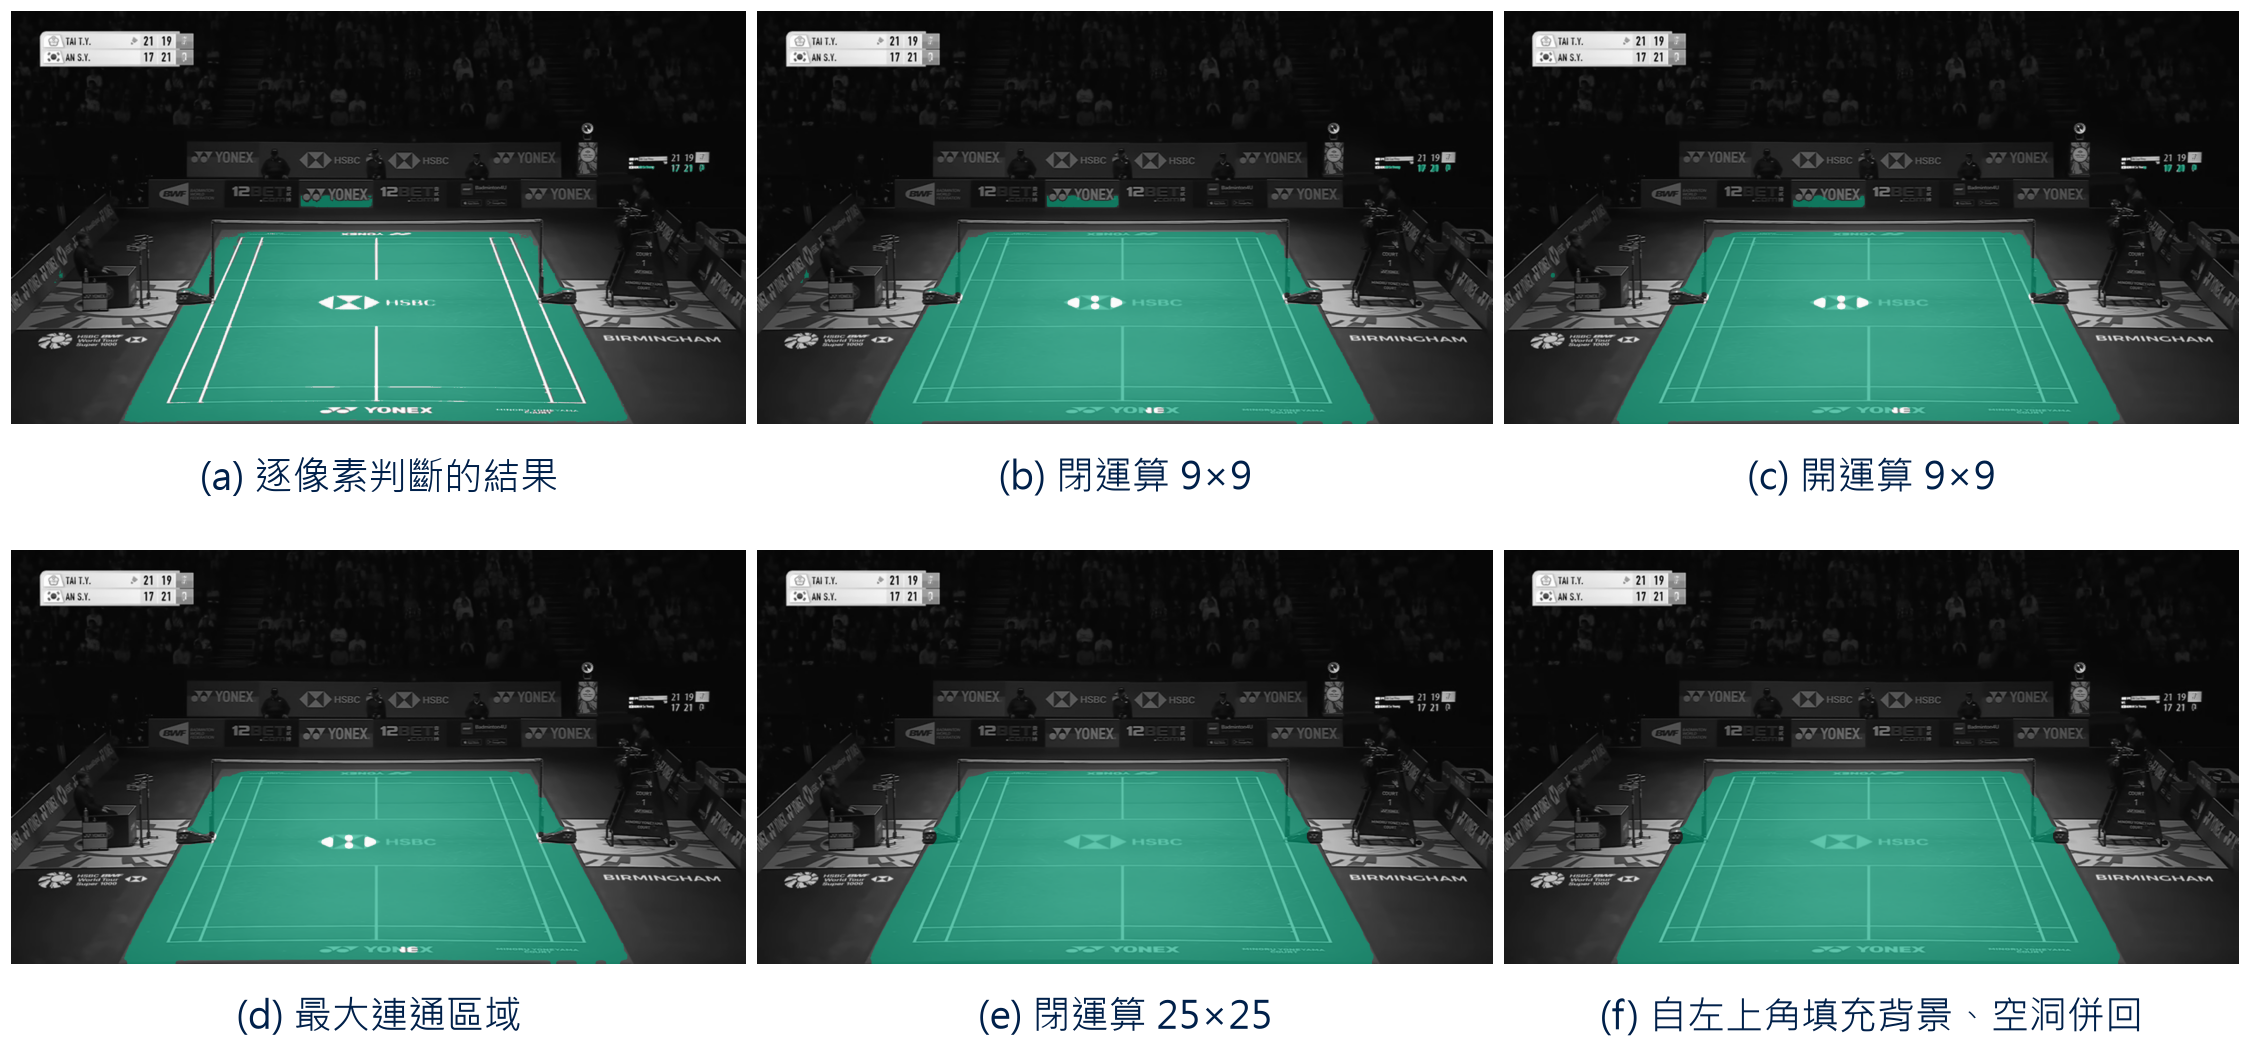
\includegraphics[width=\linewidth]{court_detection/morphology.png}
  \caption{形態學清理、最大連通區域與空洞填補各階段的遮罩變化}
  \label{fig:morphology}
\end{figure}

本步驟實際產生的不只一張遮罩。除上述色度版本外，另備一個紋理版本，在色度條件之外再加一道局部亮度標準差門檻，只留下平滑區域，用以濾掉與場地同色卻花紋雜亂的地面贊助商圖樣（\figref{fig:texture-gate}）。另有一個低色度版本，在整體畫面色度過低、色度判準失效時改以亮度相似度取代色度。這些版本不互相取代，而是一併往下送，構成後續多假設並行的二至三組遮罩。

\begin{figure}[H]
  \centering
  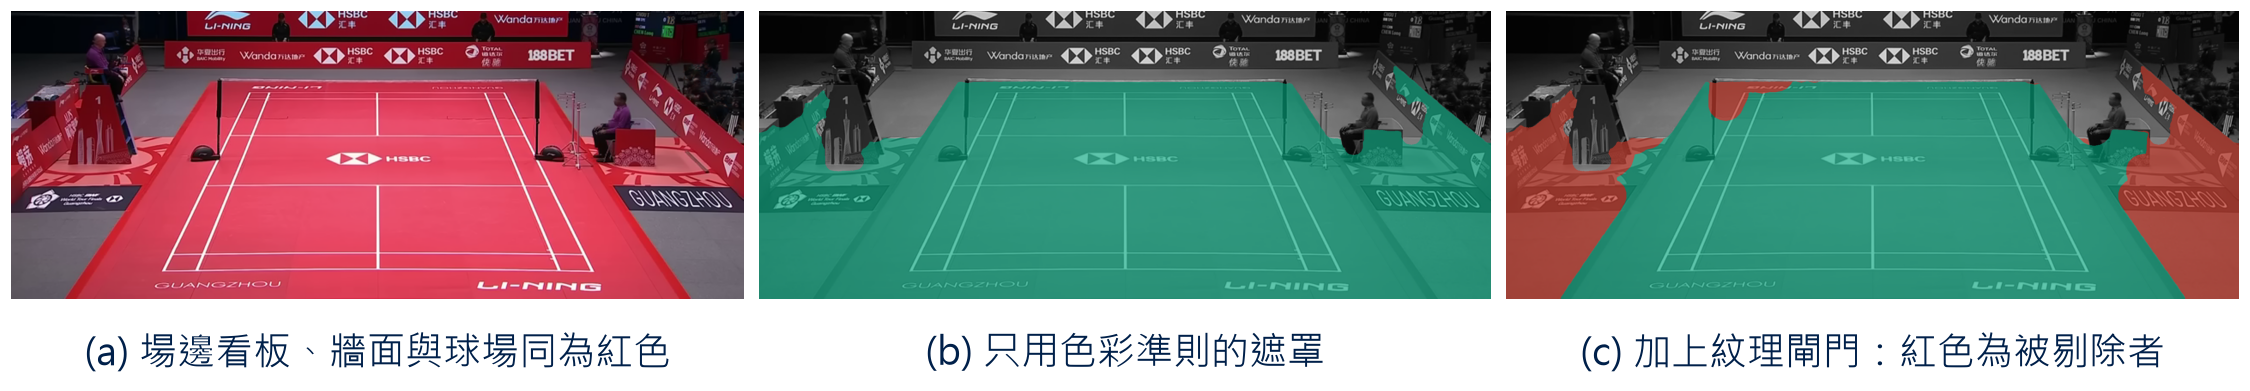
\includegraphics[width=\linewidth]{court_detection/texture_gate.png}
  \caption{場邊看板與球場同色時，紋理版本剔除色度版本誤納的區域}
  \label{fig:texture-gate}
\end{figure}

\subsubsection{場線偵測}

本步驟要在前一步的遮罩範圍內找出球場線，過程分四段，取出屬於線的像素、把像素組織成線段、濾除不屬於球場的線段、合併接近的線段。

取線像素不靠色彩，轉播素材的曝光與白平衡各異、場線的絕對色值並不固定。使用局部亮度突起，一個像素若比水平（或垂直）方向兩側都亮出門檻 $\tau$，即屬近垂直（或近水平）的線像素，$P_h$、$P_v$ 取聯集，比較距離 $d$ 須大於線寬（\figref{fig:line-pixels}）：
\begin{gather}
  P_h(x,y) = \big[\,G(x,y)-G(x-d,y) > \tau\,\big] \wedge \big[\,G(x,y)-G(x+d,y) > \tau\,\big] \\
  P_v(x,y) = \big[\,G(x,y)-G(x,y-d) > \tau\,\big] \wedge \big[\,G(x,y)-G(x,y+d) > \tau\,\big]
\end{gather}

\begin{figure}[H]
  \centering
  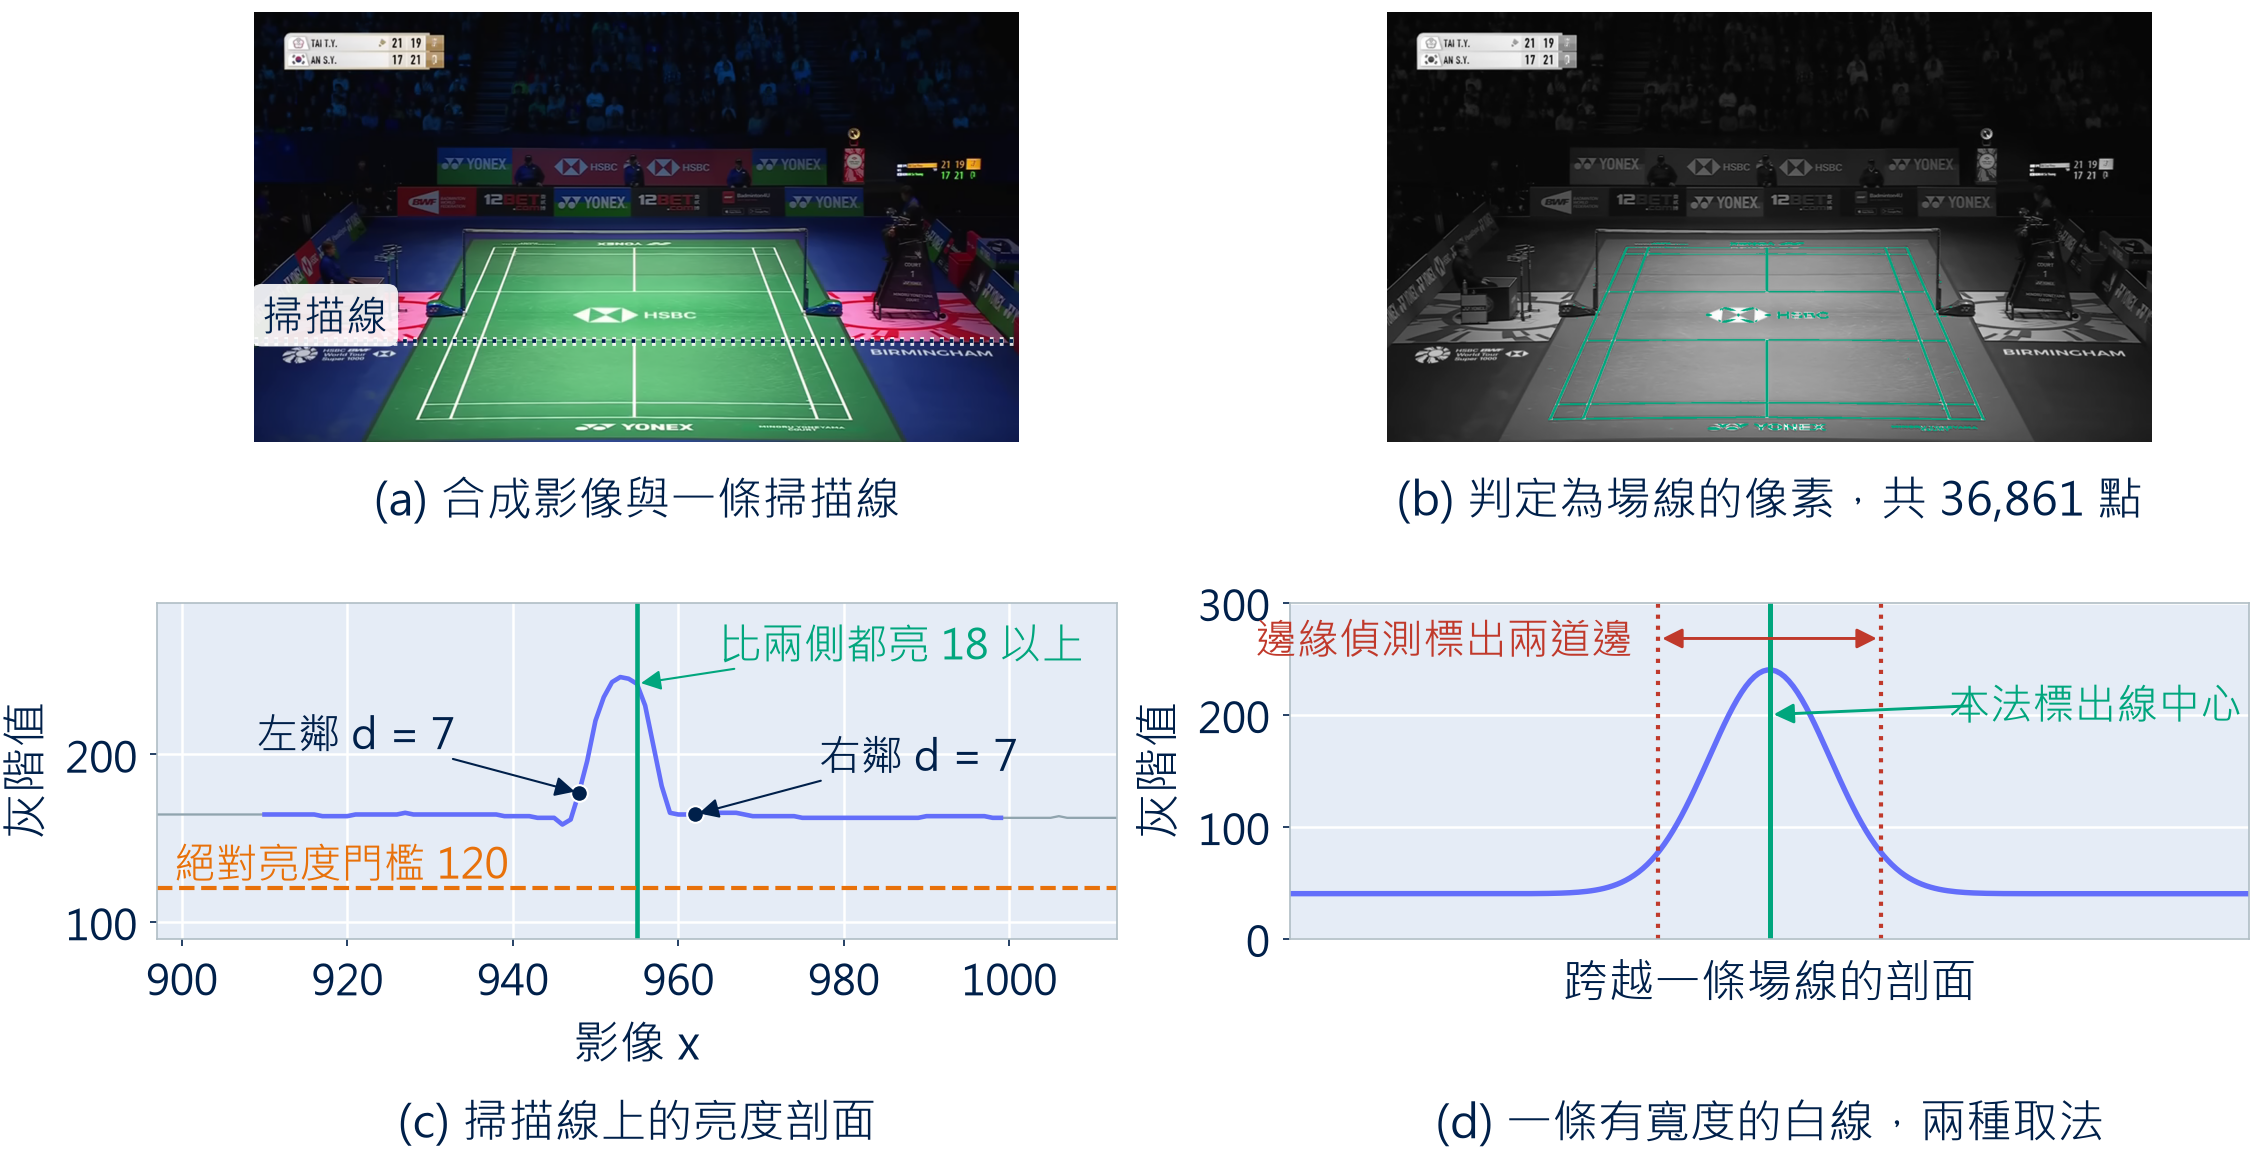
\includegraphics[width=\linewidth]{court_detection/line_pixels.png}
  \caption{局部亮度突起與場線像素的萃取結果}
  \label{fig:line-pixels}
\end{figure}

上一步的輸出是散落的像素，以機率霍夫轉換（PPHT，\texttt{cv2.HoughLinesP}）把共線者組織成線段（\figref{fig:hough-families}）。場線常因球員殘影、地面反光與遮罩侵蝕而斷開，霍夫轉換靠投票決定共線性、不依賴像素連通，能跨越這些缺口。

\begin{figure}[H]
  \centering
  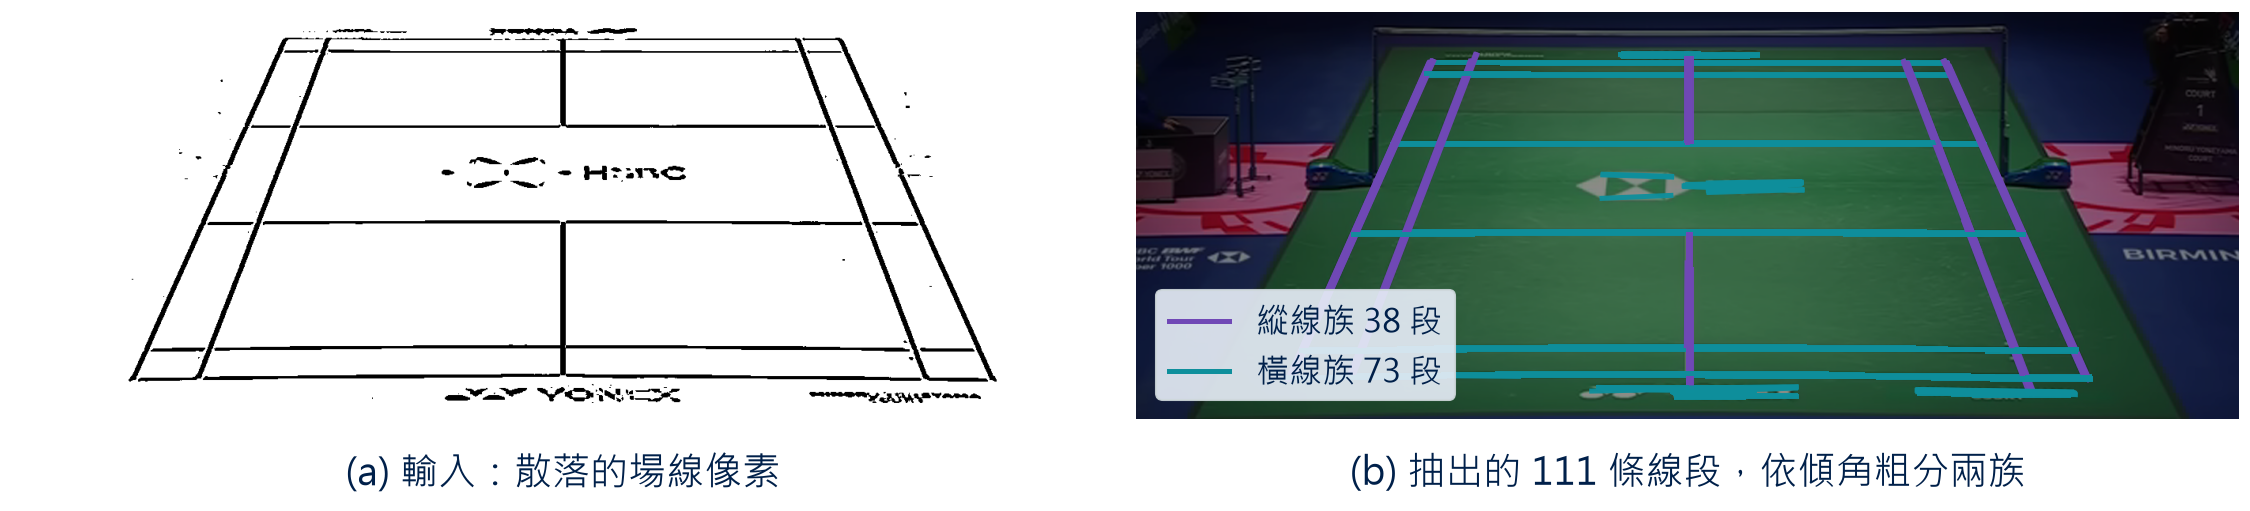
\includegraphics[width=\linewidth]{court_detection/hough_families.png}
  \caption{霍夫線段與兩族的角度粗分}
  \label{fig:hough-families}
\end{figure}

粗分後仍混有地面贊助商圖樣等非球場線段，以透視幾何篩選。球場的 12 條線分屬兩組平行線，在畫面上各自通過一個消失點。找消失點是離群比例可能很高的穩健估計問題，採 RANSAC，隨機取兩條線段、以交點為候選消失點，統計族內有多少線段方向指向它（以線段長度加權），重複數百次取支持度最高者（\figref{fig:vp-ransac}）。

\begin{figure}[H]
  \centering
  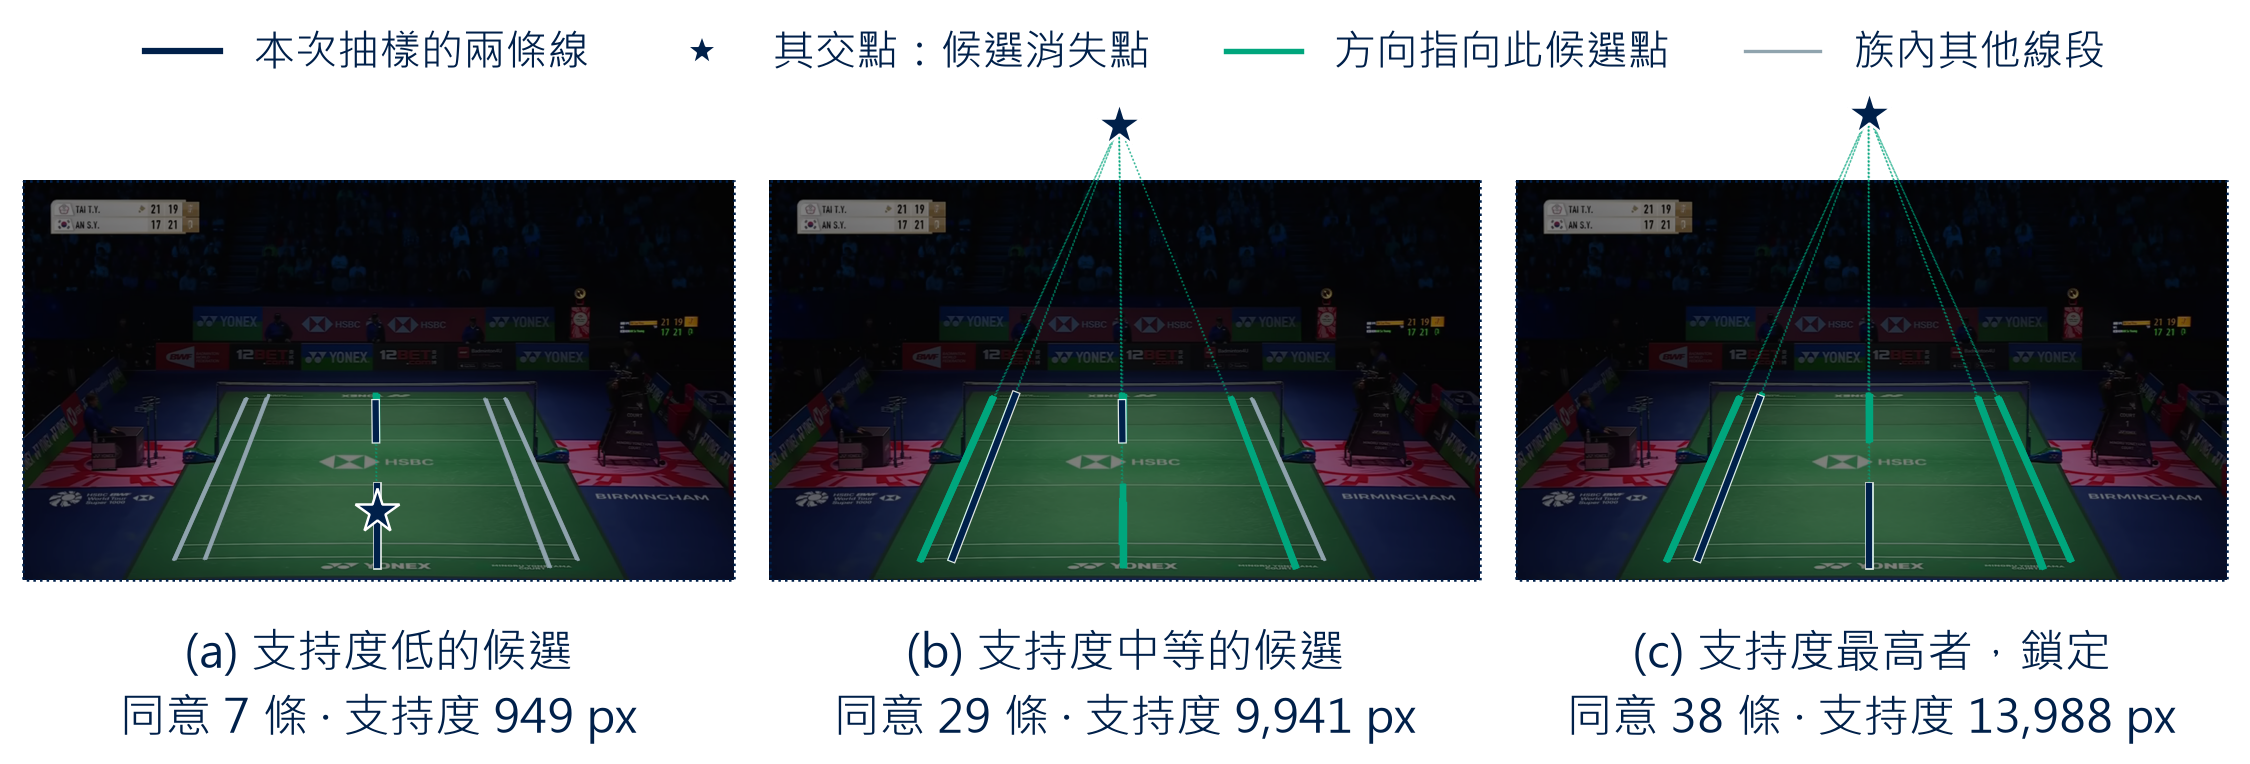
\includegraphics[width=\linewidth]{court_detection/vp_ransac.png}
  \caption{消失點 RANSAC 三次抽樣的候選點與其支持度}
  \label{fig:vp-ransac}
\end{figure}

球網遮擋常把一條球場線拆成方向略有出入的數段，同一條物理線會以不同位置重複參與運算，故先合併。同族線段方向相近、只在垂直於該方向的位置上分開，取一條參考線把每條線段化為一維位置，位置相近者歸為一簇，每簇以最小平方擬合出一條代表線。數百條線段因此收斂成十餘條物理線，既去除重複，也把後續窮舉的組合數壓到可行範圍（\figref{fig:line-merge}）。

\begin{figure}[H]
  \centering
  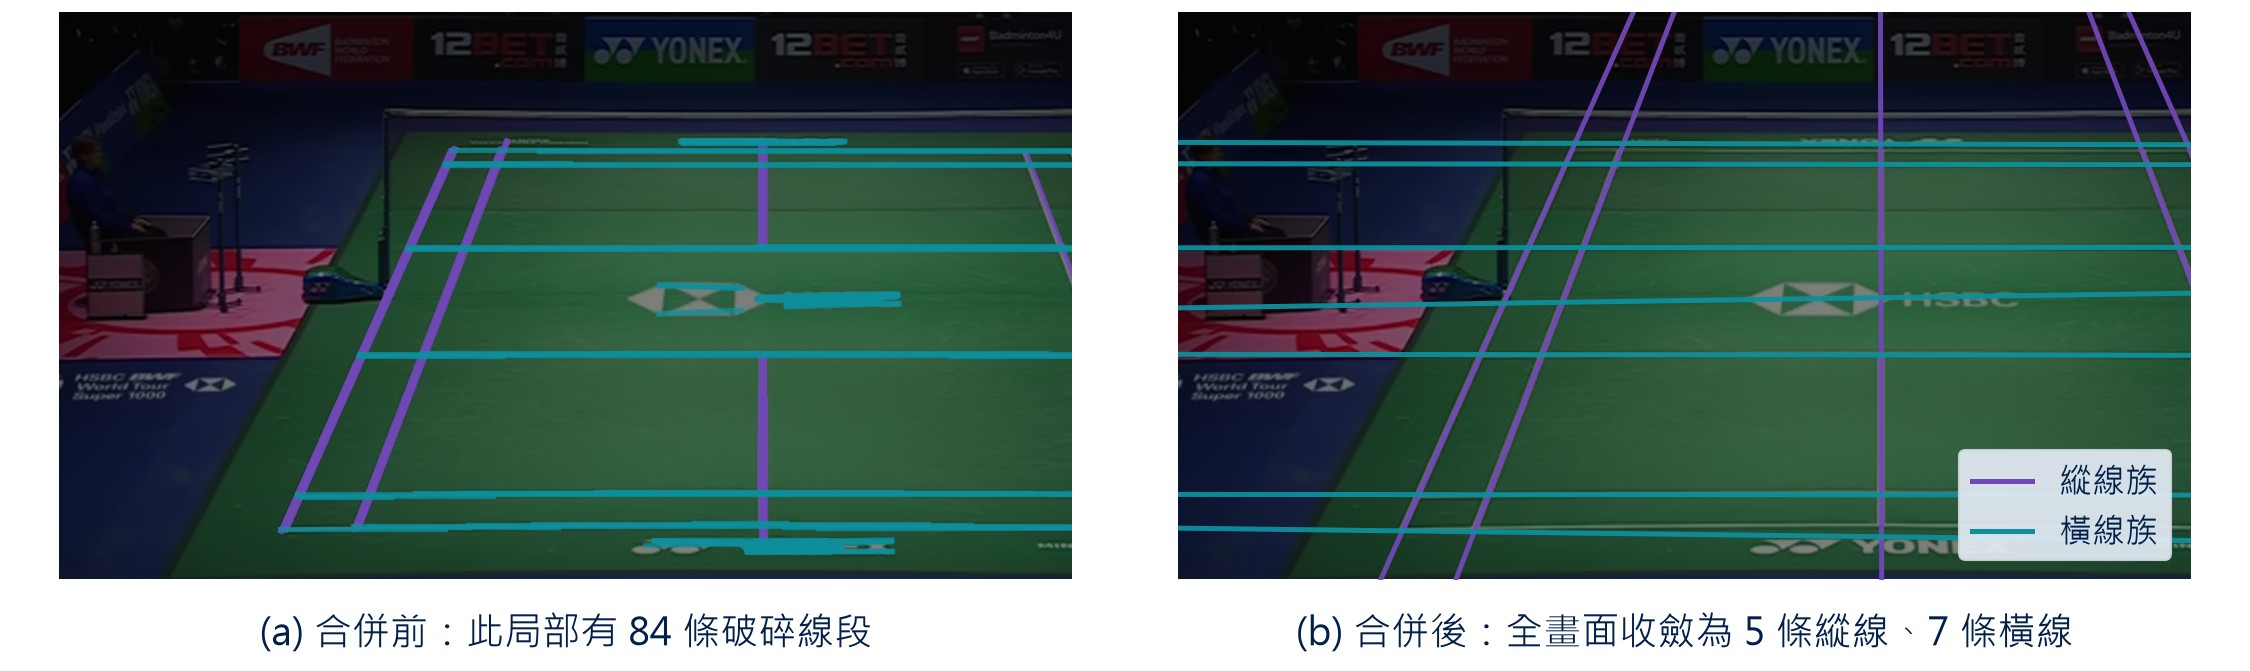
\includegraphics[width=\linewidth]{court_detection/line_merge.png}
  \caption{同族線段合併的前後對比}
  \label{fig:line-merge}
\end{figure}

\subsubsection{單應性與吻合度評分}

本步驟解決「如何由四角解出單應性、如何量化一組四角的好壞」的問題。

羽球場的尺寸與 12 條場線位置皆為已知常數，因此可預先建立球場模型座標：5 條縱線對應固定的 $x$ 值，7 條橫線對應固定的 $y$ 值。將模型四角與影像中偵測到的四角建立對應後，即可用 DLT 解出單應性 $\mathrm{H}$，再由 $\mathrm{H}$ 將模型中的 12 條場線與 16 個交點一併投影至影像。

DLT 對趨近退化的輸入不會報錯，仍會得出病態的 $\mathrm{H}$，故對每個 $\mathrm{H}$ 加設合法性檢查：四角須為有限值、不超出畫面、不退化成細條、近端底線不短於遠端（\figref{fig:valid-h}）。此檢查貫穿後續所有產生 $\mathrm{H}$ 的階段。

\begin{figure}[H]
  \centering
  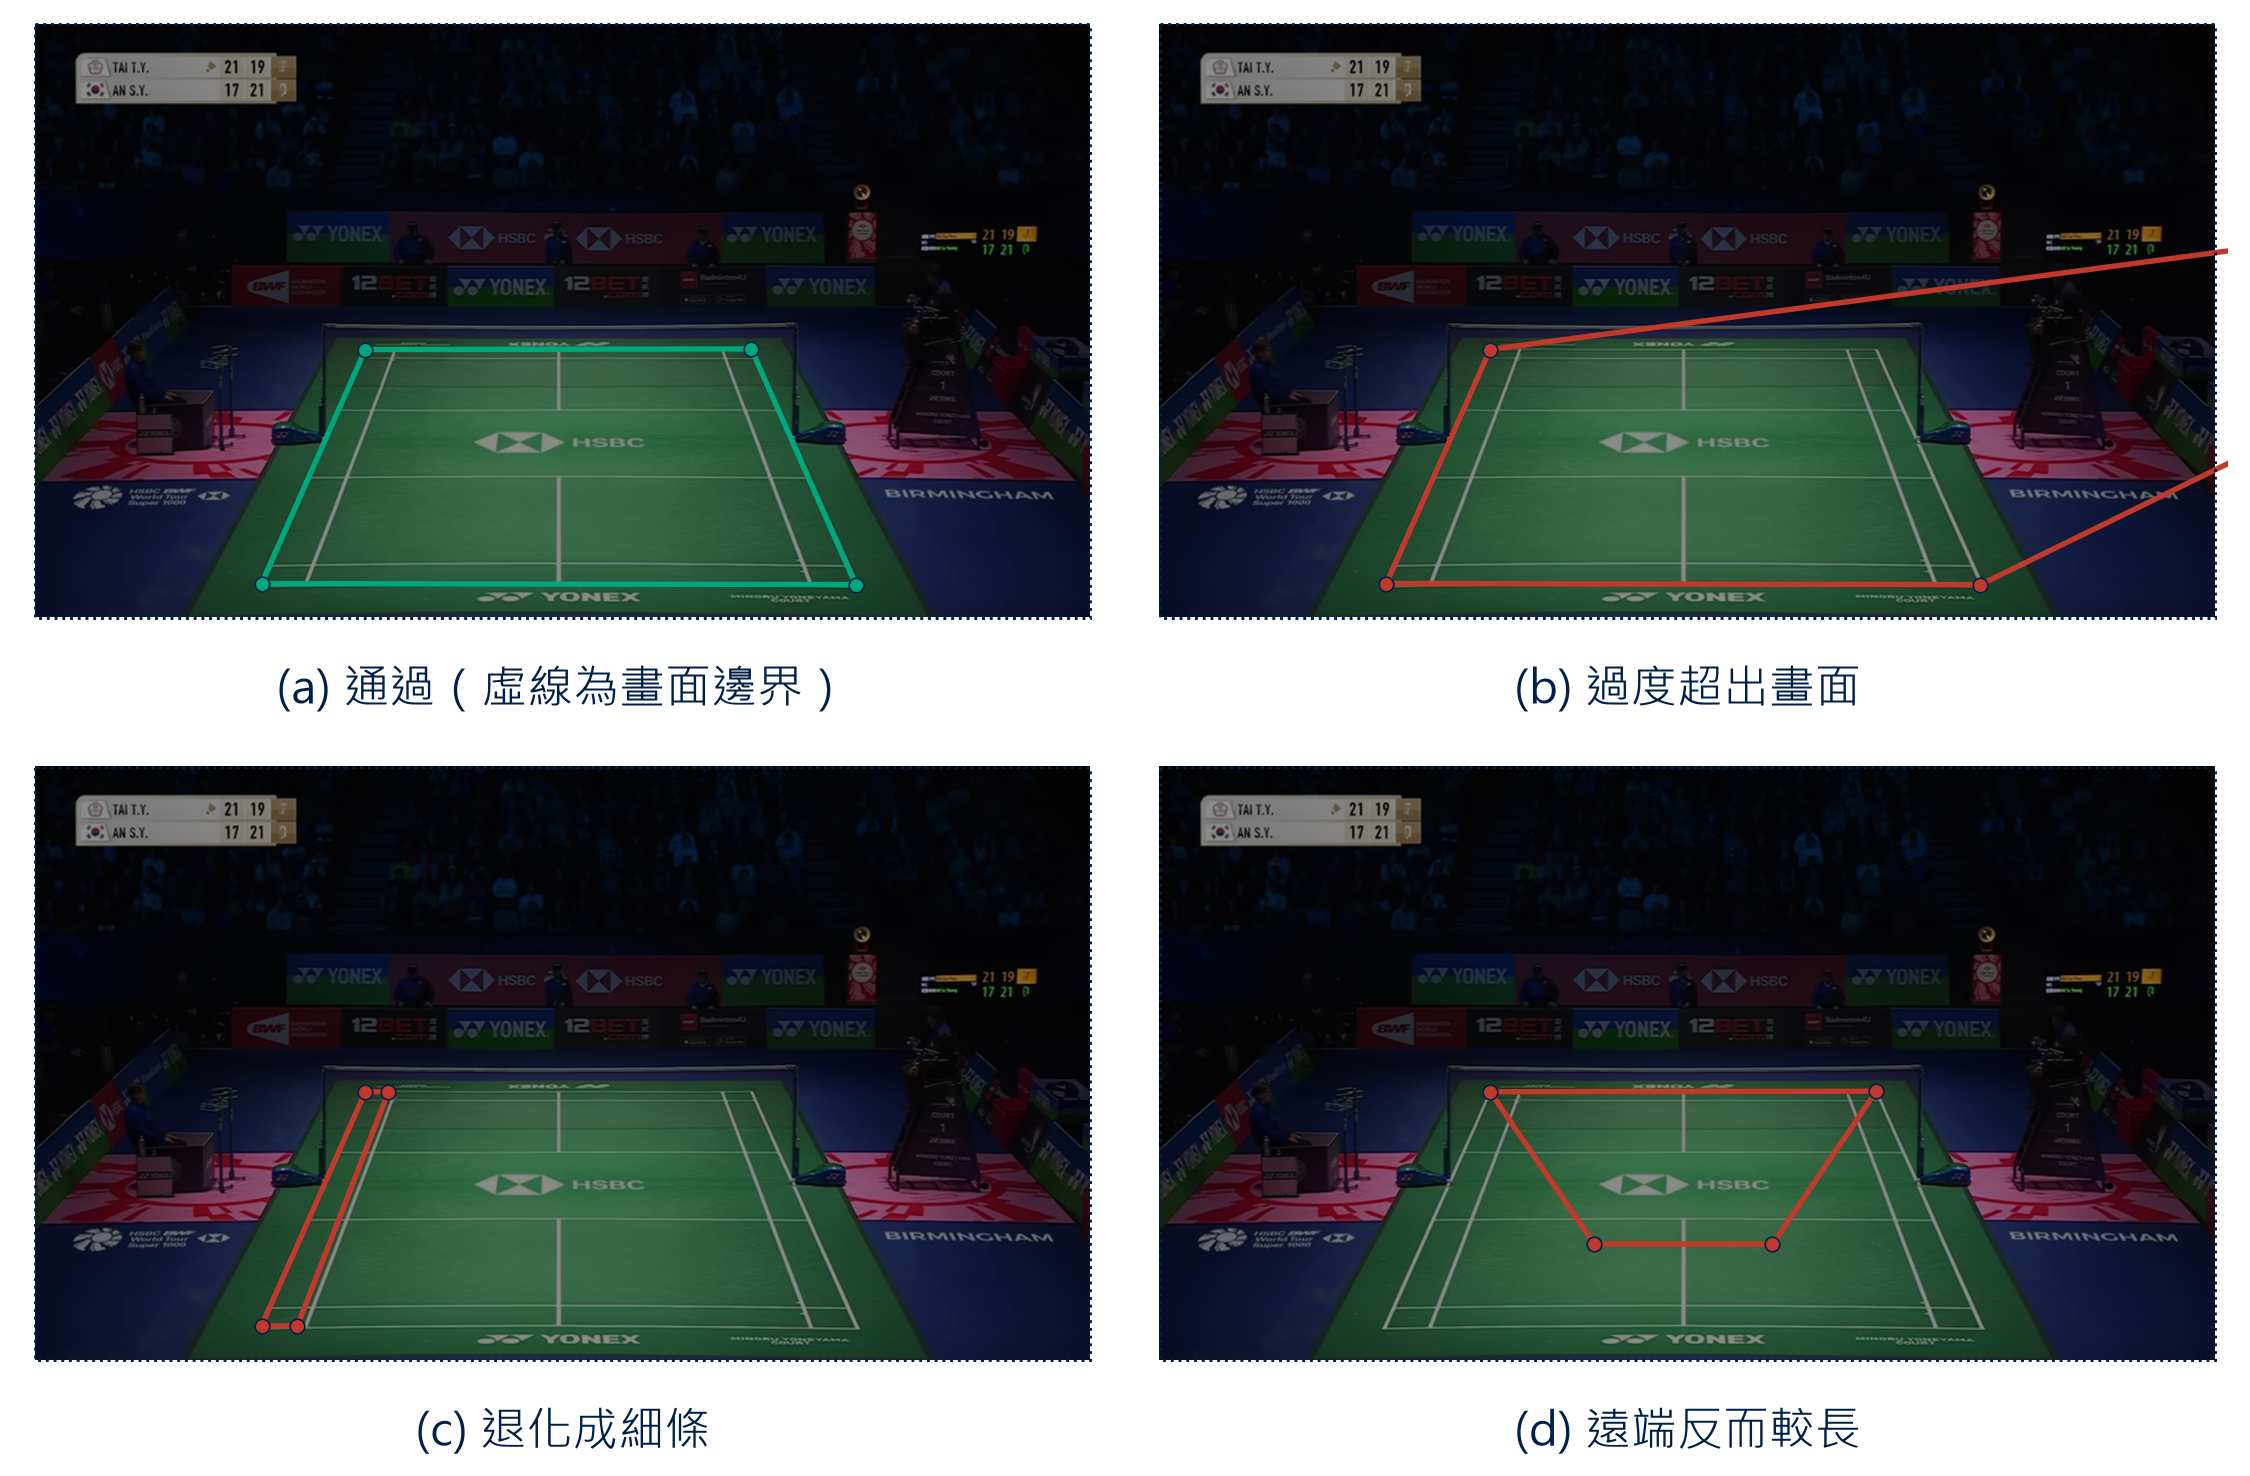
\includegraphics[width=\linewidth]{court_detection/valid_h.png}
  \caption{合法性檢查}
  \label{fig:valid-h}
\end{figure}

吻合度評分衡量 $\mathrm{H}$ 推出的網格與畫面上實際偵測到的場線像素有多吻合。單條線的覆蓋率定義為：沿線等距取若干點、投影到影像，落在最近場線像素容差（4 像素）內的比例（\figref{fig:distance-transform}）。總評分取「貼合度」與「廣度」兩項相乘：
\begin{equation}
  S = \underbrace{\frac{1}{12}\sum_{k=1}^{12}\mathrm{cov}_k}_{\text{貼合度}} \times \underbrace{\frac{1}{12}\big\lvert\{\,k : \mathrm{cov}_k > 0.3\,\}\big\rvert}_{\text{廣度}}
  \label{eq:court-score}
\end{equation}
此評分是整個場地偵測判斷好壞的統一依據，後續的候選選擇與邊界修正都以它裁決。

\begin{figure}[H]
  \centering
  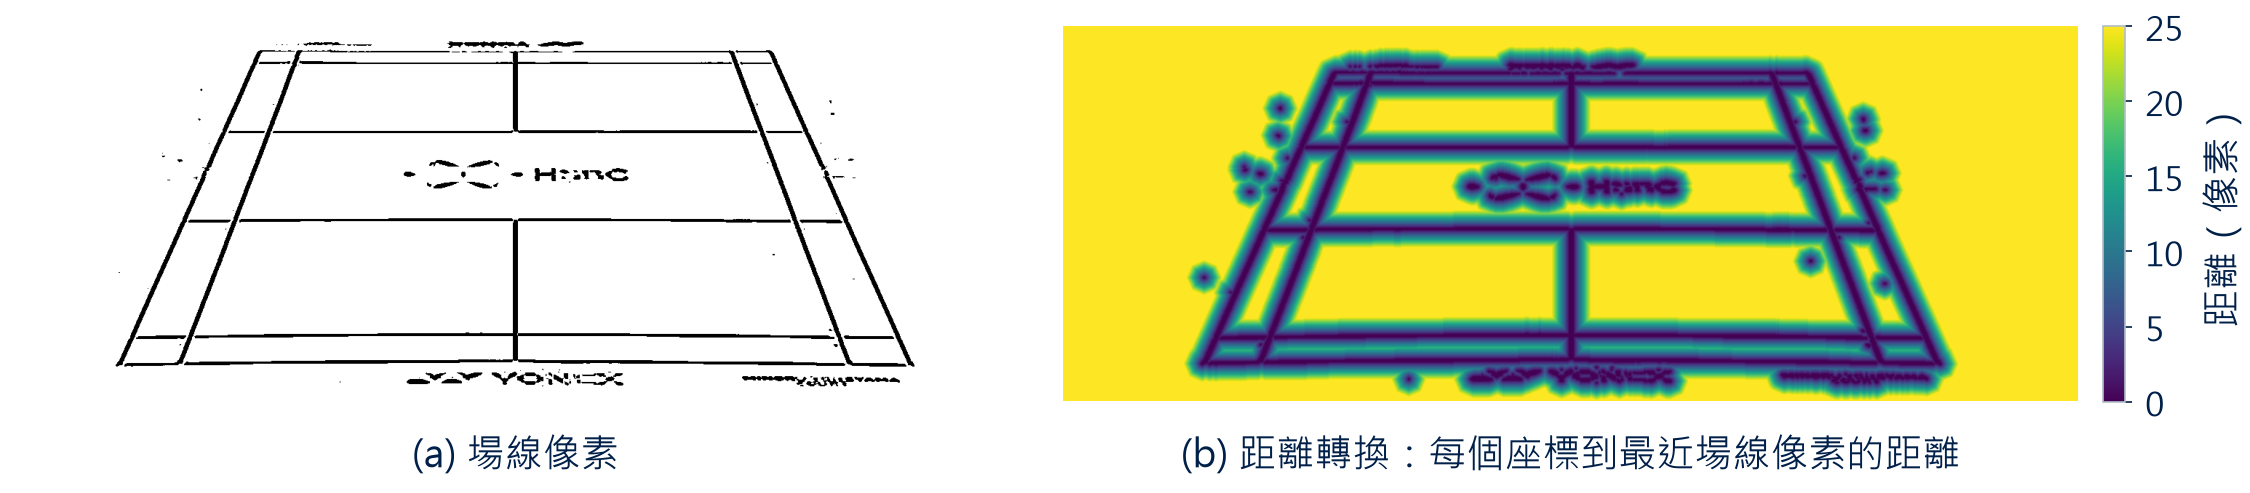
\includegraphics[width=\linewidth]{court_detection/distance_transform.png}
  \caption{場線像素與其距離轉換圖}
  \label{fig:distance-transform}
\end{figure}

\subsubsection{外角候選}

四角須由偵測到的線或遮罩推導，任一種推導都有其失效條件，故本模組並行三種來源、各給一組候選，三者的失效條件互不重疊。

\textbf{網格枚舉（主要方法）：}從候選縱線任取兩條作左右邊界、橫線任取兩條作上下邊界，四線相交得一組四角，枚舉所有 $\binom{10}{2}\times\binom{12}{2}=2970$ 組合，取 12 線網格吻合度最高者（\figref{fig:grid-search}）。穩健的關鍵在於以最可靠的內部線反推最不可靠的外角，等於讓發球線與中線一起投票決定四角。

\begin{figure}[H]
  \centering
  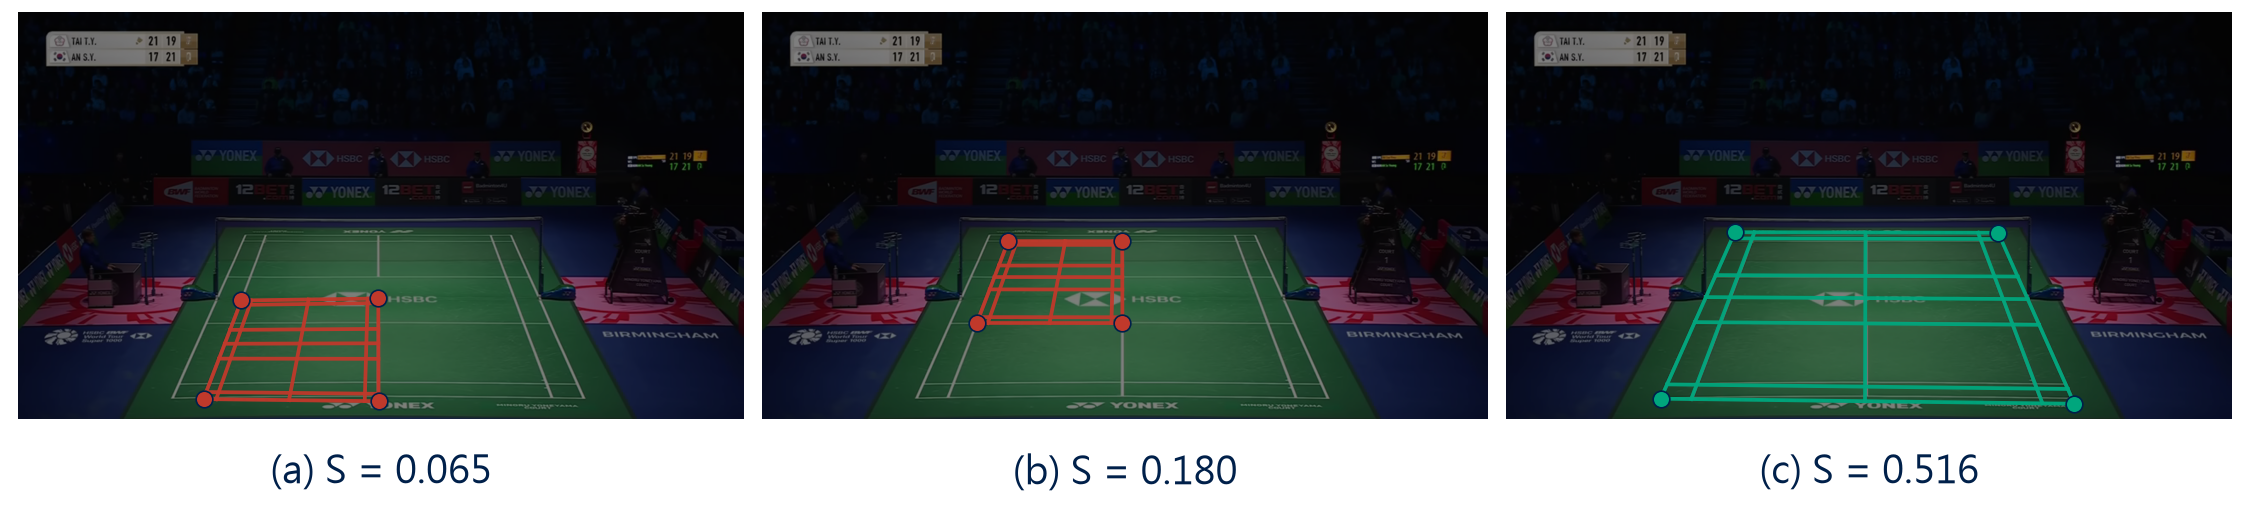
\includegraphics[width=\linewidth]{court_detection/grid_search.png}
  \caption{網格枚舉的候選與其吻合度評分}
  \label{fig:grid-search}
\end{figure}

\textbf{極端線相交：}在兩族中各取最外側的兩條線相交得四角，最直接，但要求那四條極端線全部正確，而外緣線最難偵測，故僅作第二來源。它的失效條件與網格枚舉不同，能在枚舉搜尋空間無正解時補位。

\textbf{遮罩凸包：}改用遮罩形狀，取面積最大的外輪廓、求凸包並簡化為多邊形，再由頂點座標的極值取出四角。它不需任何場線，但遮罩邊界經形態學處理與空洞填補、未必等於球場外緣，精度最低，僅在前兩者都產生不出合法 $\mathrm{H}$ 時作為備援。

\subsubsection{角點重估與邊界修正}

前一步的四角只由少數代表線相交而得，影像中大量場線像素尚未參與，本步驟用上全部線像素把結果調準，分兩階段。

\textbf{以 ICP 重估單應性：}難點在建立線像素與球場模型的對應，影像中場線因透視而方向各異，難以直接配對。利用前一步的近似 $\mathrm{H}$，把每個線像素反投影回球場座標，那裡的縱線是 $x$ 為定值、橫線是 $y$ 為定值的直線，量出該像素離哪條最近即建立對應。再用全部點對重解 $\mathrm{H}$、以新 $\mathrm{H}$ 更新對應，反覆逼近。點對數以千計，採 RANSAC 版本把配錯到相鄰線的像素當離群值排除，對應的距離門檻隨迭代由寬到窄（\figref{fig:icp}）。

\begin{figure}[H]
  \centering
  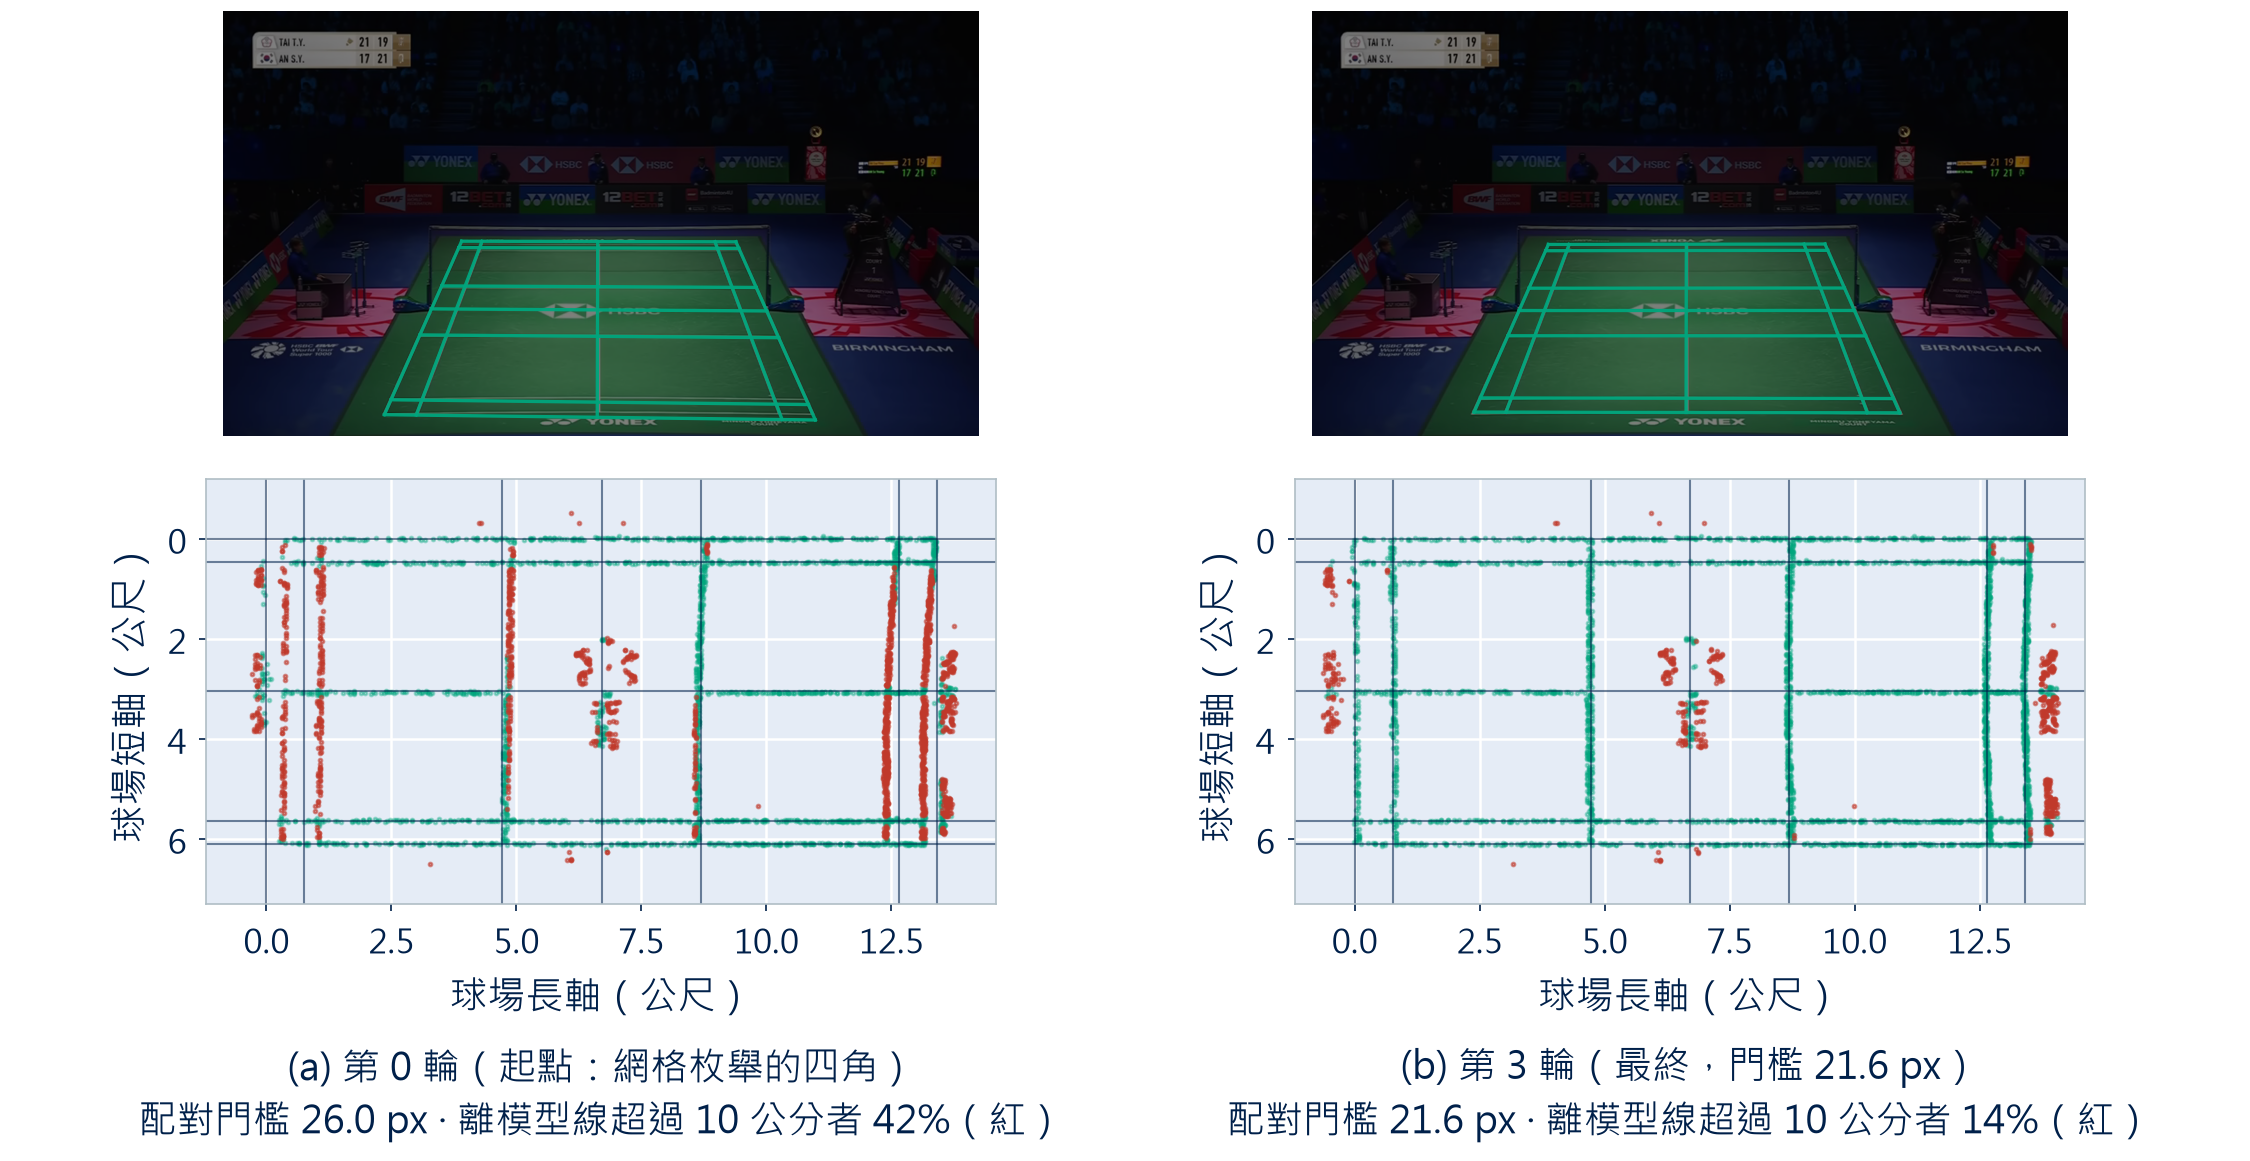
\includegraphics[width=\linewidth]{court_detection/icp.png}
  \caption{ICP 第一輪與最終輪的網格與反投影殘差}
  \label{fig:icp}
\end{figure}

\textbf{邊界修正：}透視壓縮下球場遠端的內、外邊界在畫面上靠得很近，全域解無從分辨，外邊界可能整條鎖到內側線上。本步驟只動四條外邊界，把某條投影線附近的像素依「離線多遠」投到一維直方圖，每條平行線形成一個峰，二維的找線因此降為一維的找顯著峰（\figref{fig:perp-profile}）。遠端刻意偏取最外側的峰重新擬合邊界，因為兩種誤差不對稱，外邊界略往場外時場內物體的相對位置仍成立、下游影響有限，一旦鎖進內側則截斷場內內容、不可逆。搜尋帶寬由寬到窄逐級縮小。這是帶方向的推測，故結果不直接採用，而是回到吻合度評分重算，只有分數未明顯變差才取代原解（\figref{fig:boundary-refine}）。

\begin{figure}[H]
  \centering
  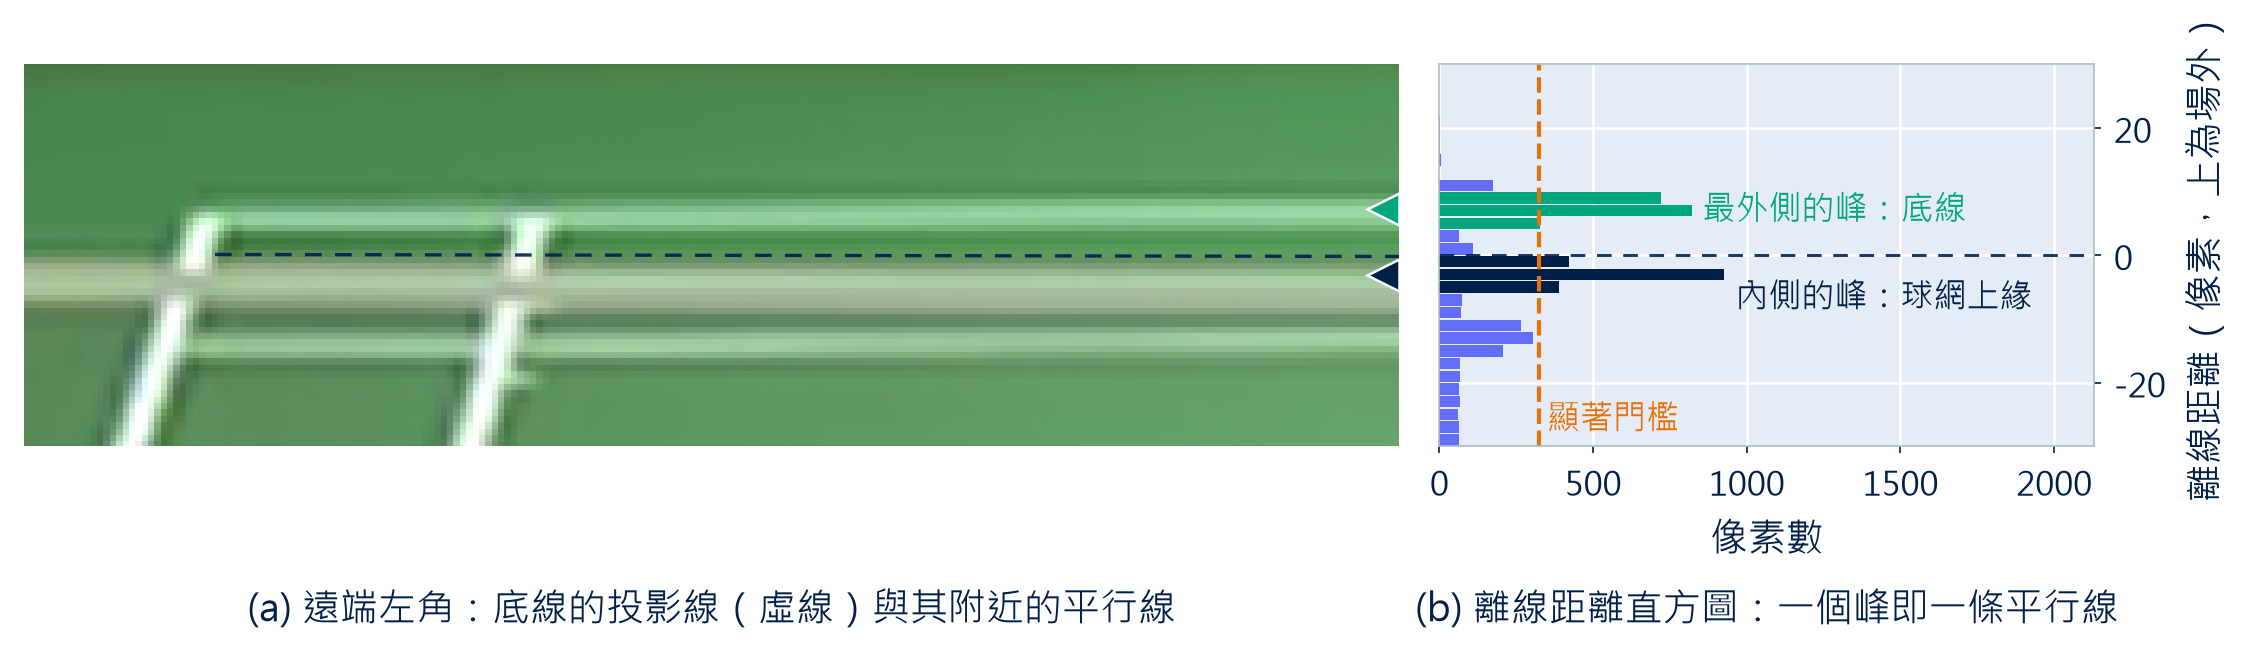
\includegraphics[width=\linewidth]{court_detection/perp_profile.png}
  \caption{投影線的鄰近像素與其離線距離直方圖}
  \label{fig:perp-profile}
\end{figure}

\begin{figure}[H]
  \centering
  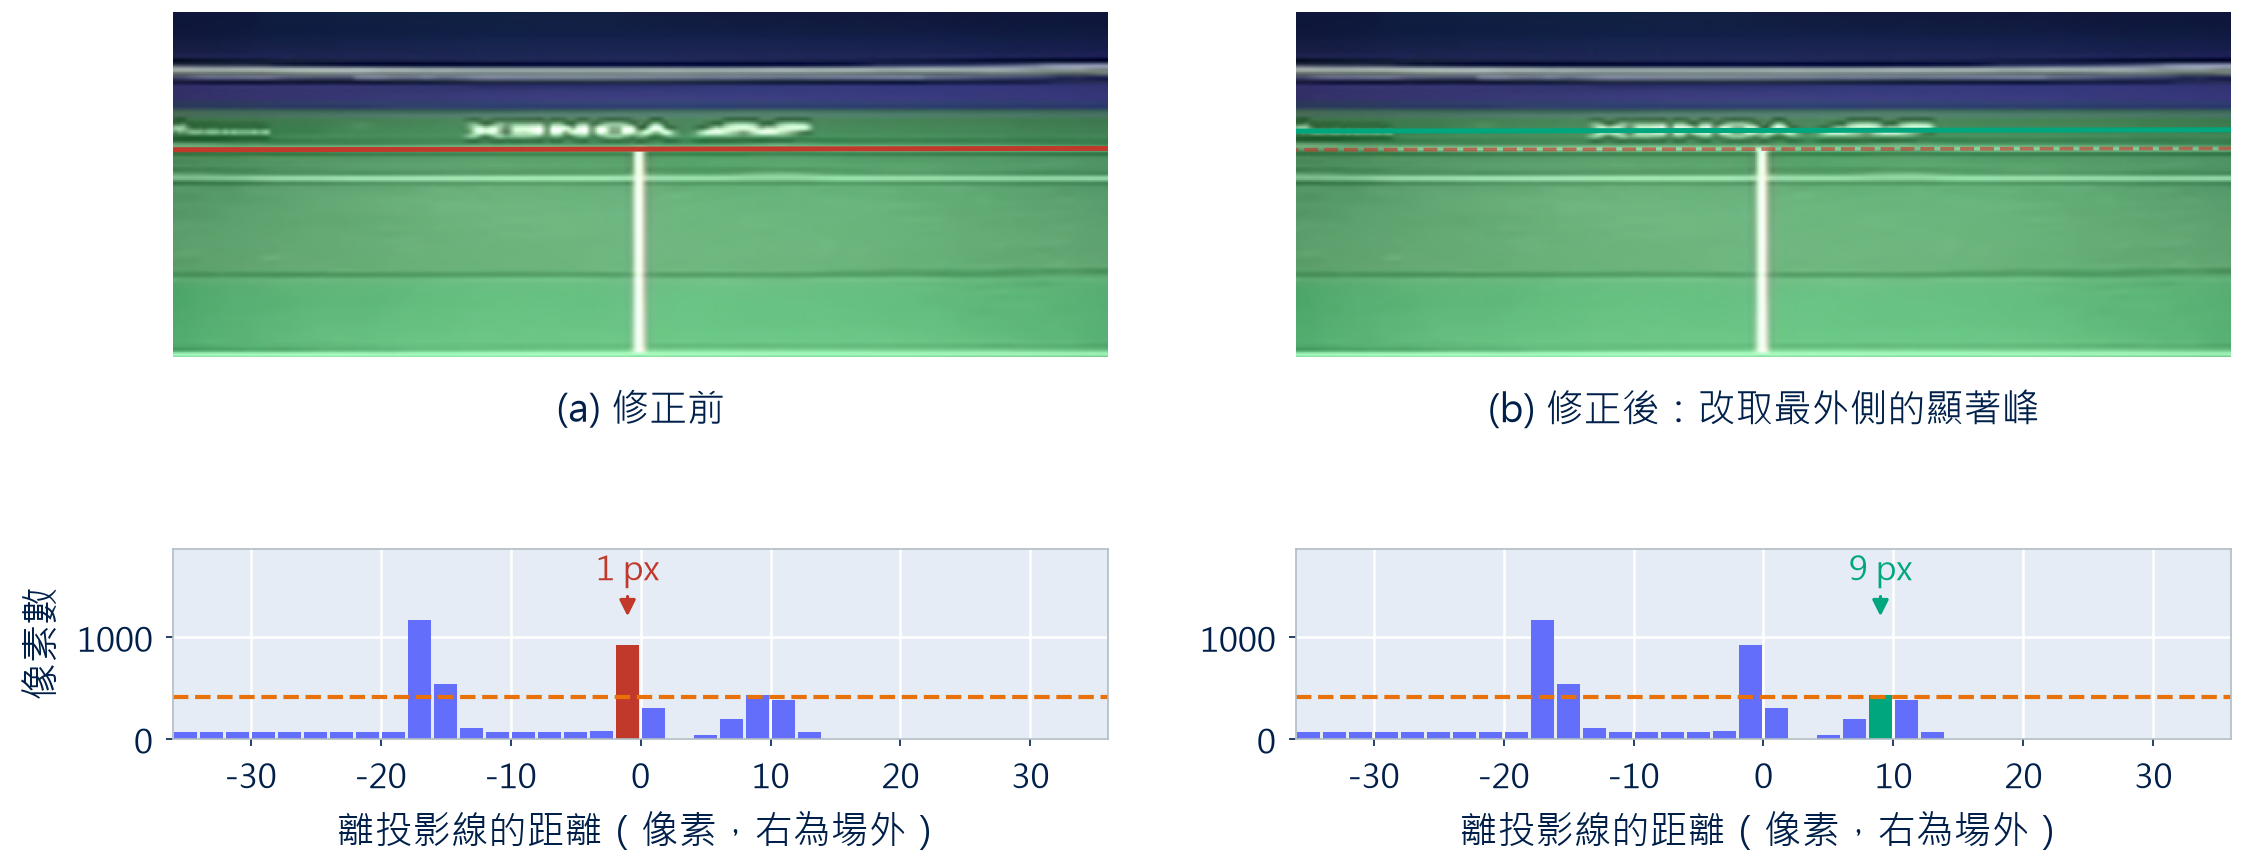
\includegraphics[width=\linewidth]{court_detection/boundary_refine.png}
  \caption{遠端底線由內側峰改取最外側峰的前後對比}
  \label{fig:boundary-refine}
\end{figure}

\subsubsection{結果驗證與評分}

前述步驟以多假設並行：球場區域定位產生二至三組遮罩，場線偵測再對每組遮罩各給三種外角候選，故候選池大小為遮罩組數乘以三，每個候選都帶著它所依據的線像素圖。本步驟把這一池候選收斂成唯一答案，每個候選經角點重估與邊界修正後，在自己的線像素圖上算出吻合度評分，全部比較之下取最高者，其四角與單應性即為模組的最終輸出（\figref{fig:eval-pool}）。

\begin{figure}[H]
  \centering
  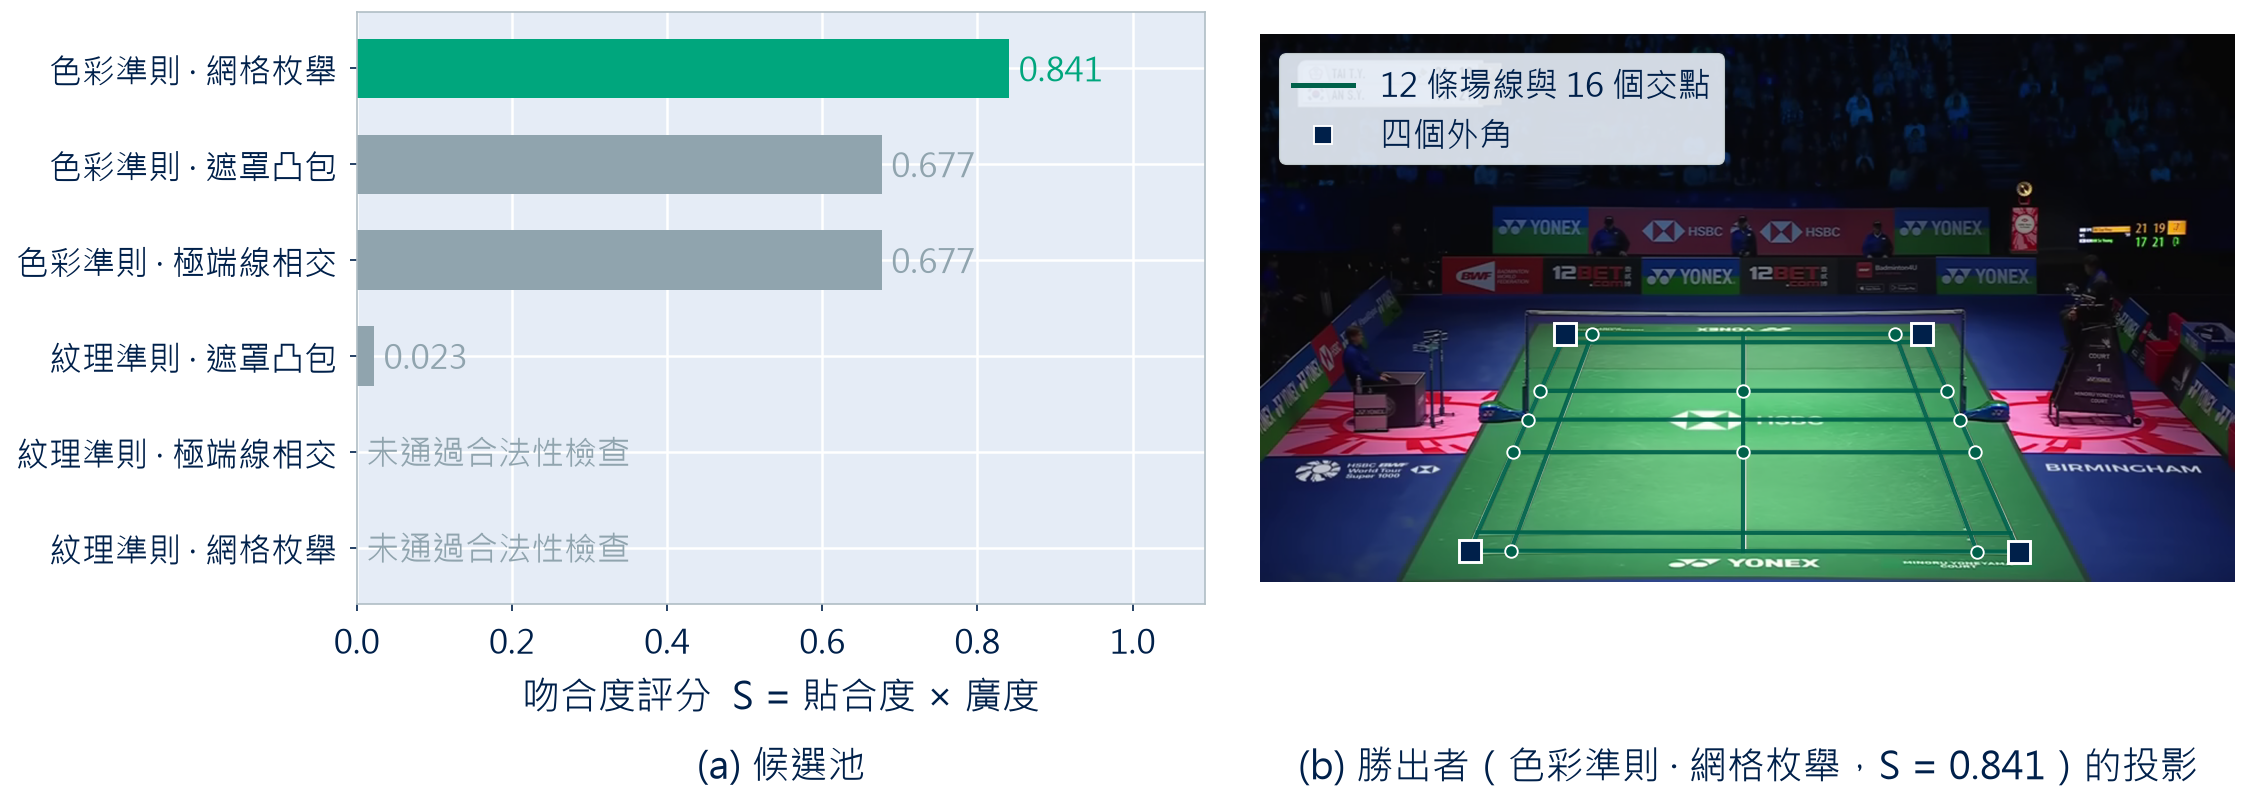
\includegraphics[width=\linewidth]{court_detection/eval_pool.png}
  \caption{候選池的吻合度評分與勝出者的投影}
  \label{fig:eval-pool}
\end{figure}

\subsection{球員骨架追蹤}
\label{sec:pose-tracking}

\subsubsection{概述}

\textbf{問題與目標：}球種分類需要球員的肢體姿態，本模組為每個片段還原場上兩名球員逐幀的骨架，作為下游球種分類的輸入。難點一是廣角轉播下球員在畫面裡常只有一兩百像素高，手肘、手腕等末端關節不易估準。難點二是畫面中除兩名球員外還有裁判、線審、球僮與觀眾，每個人都有骨架可抽，必須靠球場幾何從中認出真正的球員。

\textbf{設計重點：}本模組的核心不在姿態模型本身，而在如何從畫面中的眾多人體骨架穩定選出真正上場的兩名球員。利用球場幾何與跨幀行為自適應完成，主要有兩點做法：

\begin{enumerate}
  \item \textbf{球場座標選人：}系統把每個候選人的腳點反投影到正規化球場座標，依所在半場判定遠、近端身分，再綜合場內位置與透視校正後的身高挑選球員。
  \item \textbf{長短期時序資訊：}系統先從整場候選人的落點分布找出長時間不動的裁判、線審等靜態錨點並排除，再以短期位置記憶維持同一球員的連續身分。
\end{enumerate}

\textbf{處理流程總覽：}如\figref{fig:pose-tracking-flow}。

\begin{figure}[H]
  \centering
  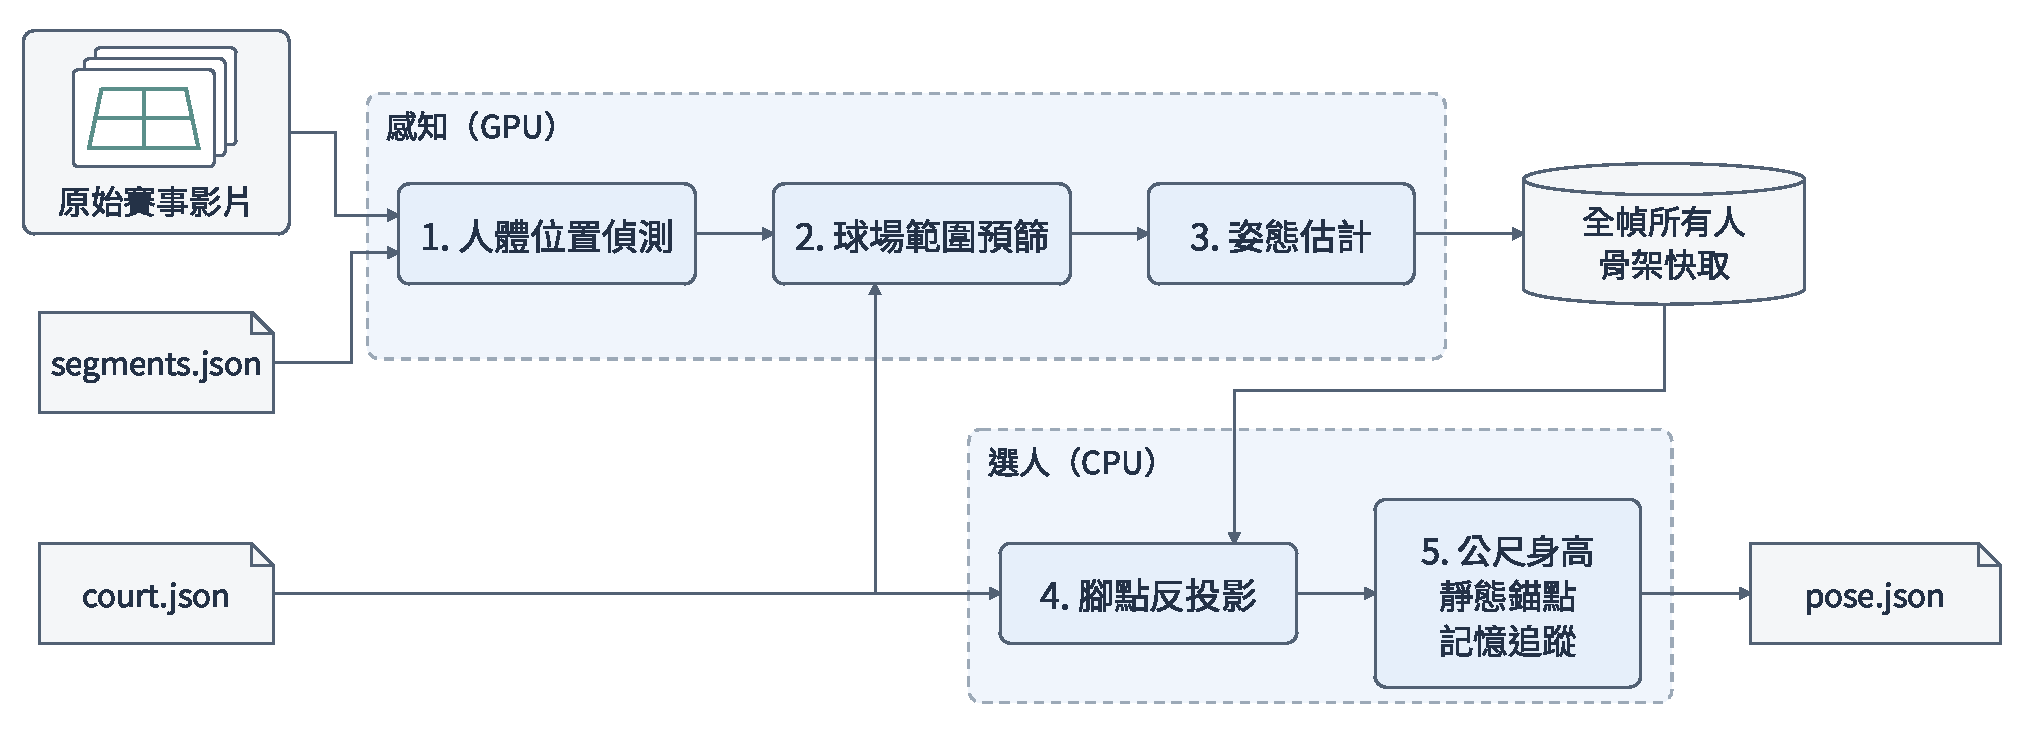
\includegraphics[scale=\flowscale]{pose-tracking.pdf}
  \caption{球員骨架追蹤處理流程}
  \label{fig:pose-tracking-flow}
\end{figure}

\subsubsection{感知：人體偵測與姿態估計}

第一階段為片段的每一幀還原畫面上所有人的骨架並快取，是整個模組的 GPU 時間瓶頸。先用人體偵測器（YOLOX）框出所有人，再採由上而下路線逐人裁切、放大回模型輸入尺寸後在滿解析度下估骨架（RTMPose），讓很小的球員仍能得到準確的關節點（\figref{fig:top-down}）。由於逐人估骨架的成本隨人數線性成長，而每幀偵到的十幾二十人裡真正相關的只有兩到四人，估骨架前先借單應性把每個人的腳點反投影回球場座標，只讓落在放寬球場範圍內者進入姿態模型。

\begin{figure}[H]
  \centering
  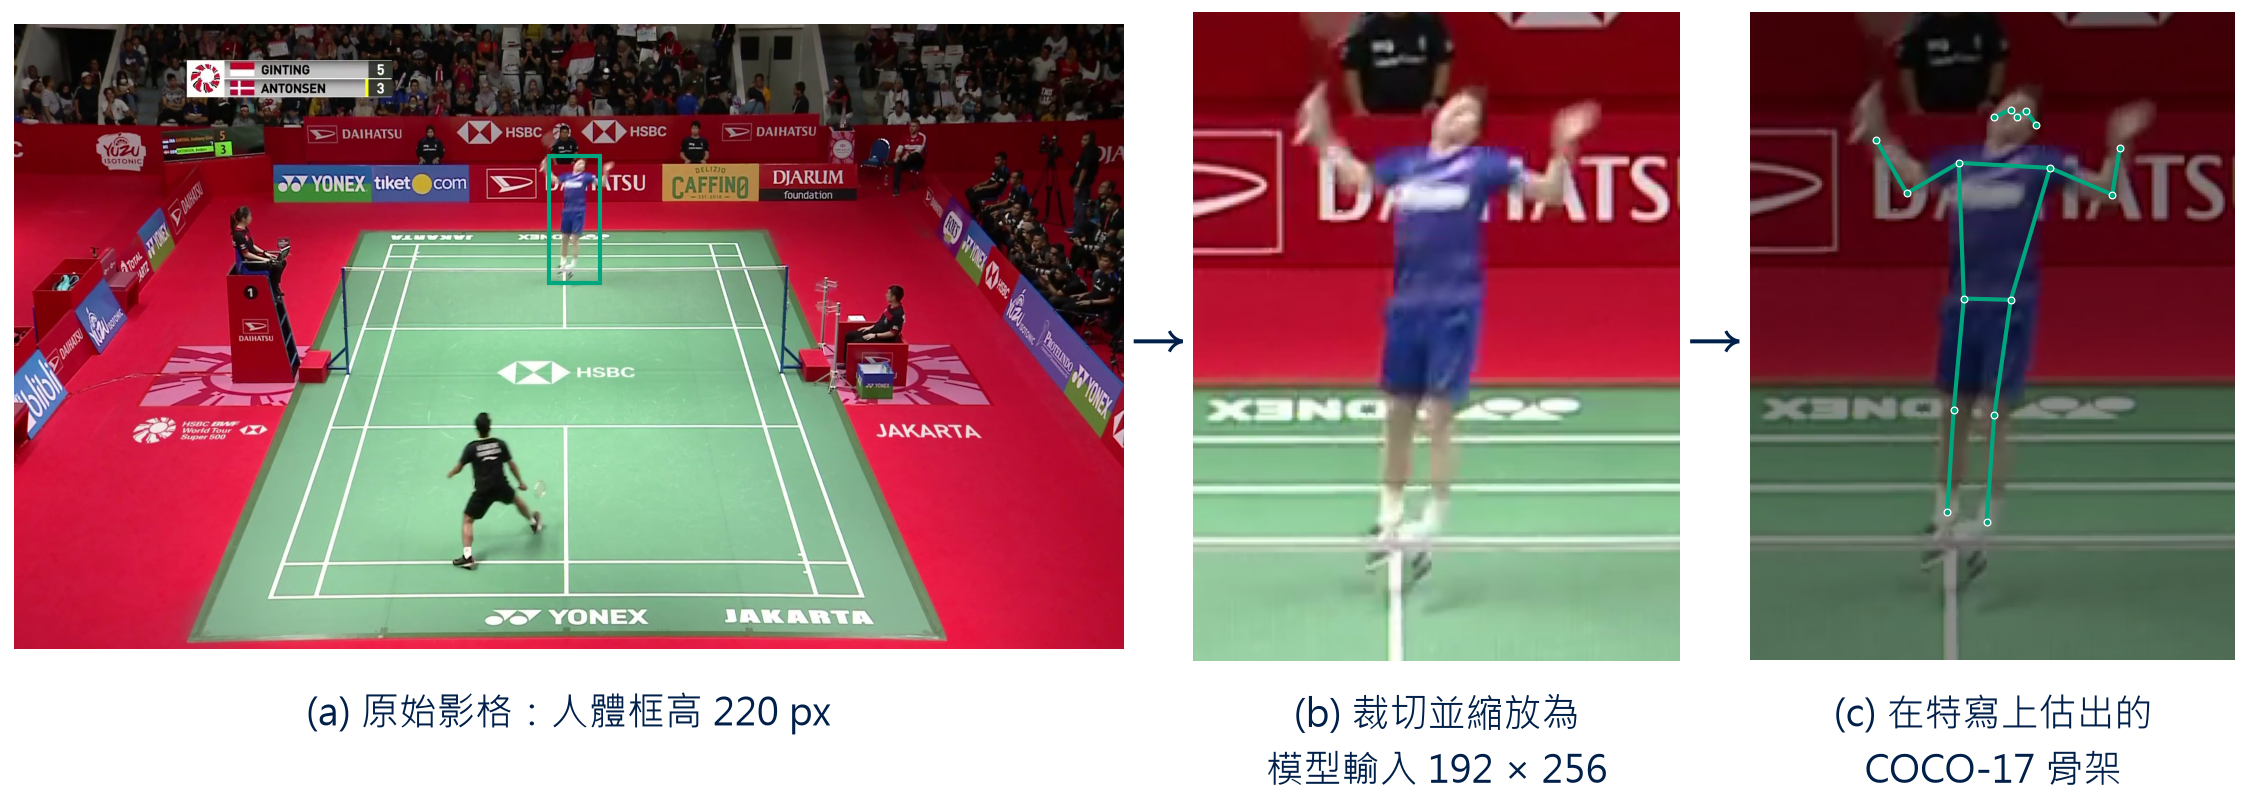
\includegraphics[width=\linewidth]{pose/top_down.png}
  \caption{由上而下，先裁切放大再估骨架}
  \label{fig:top-down}
\end{figure}

\subsubsection{選人：腳點與球網分半}

第二階段在快取好的骨架上以純幾何認出 \texttt{top}、\texttt{bottom} 兩名球員。把每個人化約為一個雙踝中點，經單應性反投影落到正規化球場座標。每一半內通過球場邊界的候選人可能不只一個，因此需要以下的排名與排除準則挑出球員。

\textbf{公尺身高排名：}不能直接選最高的人，像素高度會被透視扭曲。因此先借單應性量出畫面上每點「一公尺對應多少像素」，把候選人放到同一真實尺度上比身高。

\textbf{非對稱邊界放寬：}單應性只在地平面上成立，球員起跳殺球時腳踝離地，反投影會把腳點推到底線之外。為此把場內範圍在底線方向（縱向）放寬、邊線方向（橫向）收緊（\figref{fig:court-select}）。

\begin{figure}[H]
  \centering
  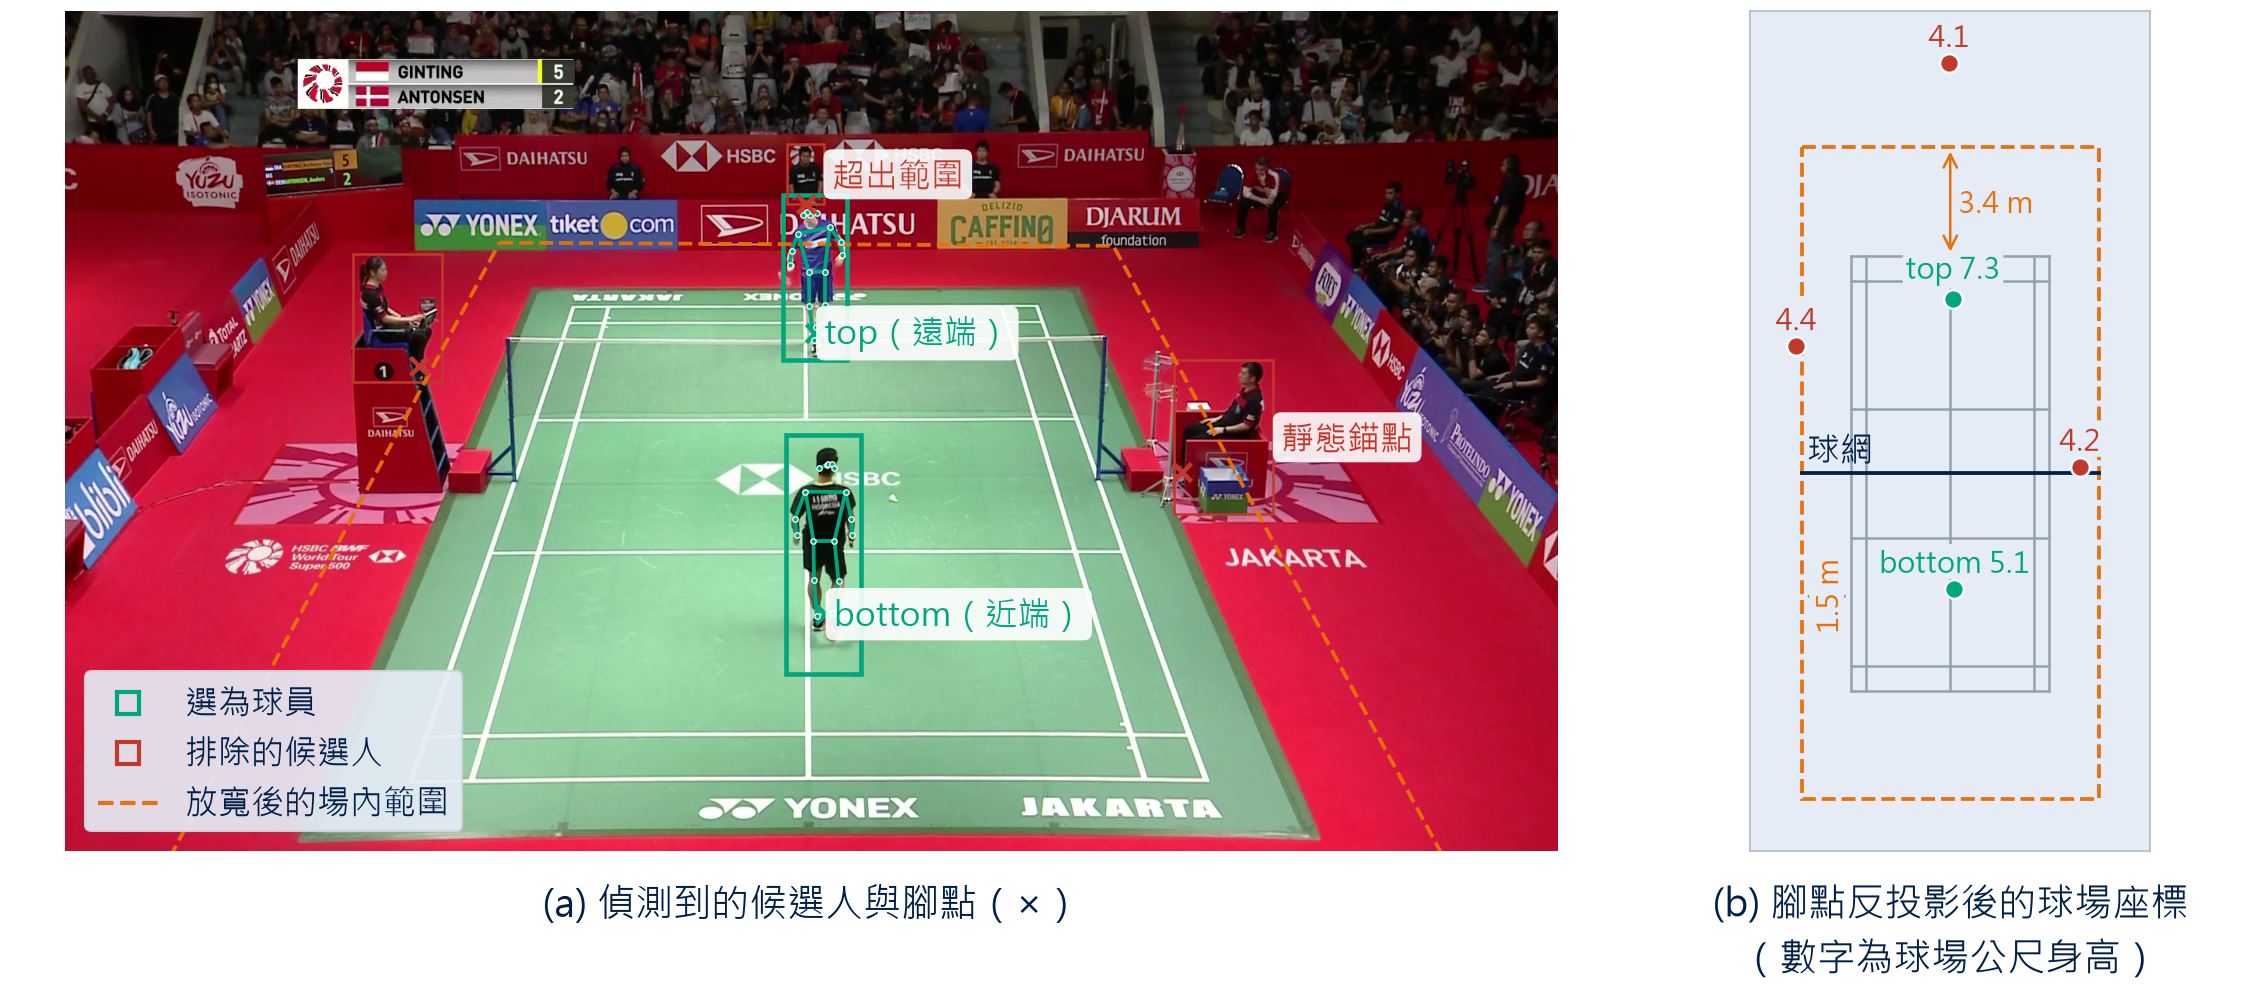
\includegraphics[width=\linewidth]{pose/court_select.png}
  \caption{腳點反投影至球場座標}
  \label{fig:court-select}
\end{figure}

\textbf{靜態錨點排除干擾：}尺寸與邊界仍擋不住一種情形，站在底線後、身高又與遠端球員相當的裁判，一旦真球員該幀被漏偵便可能頂替上來。關鍵在於是否移動，官員整場腳點落在同一處，球員則掃過整個球場。統計整場每個候選人的腳點落點，把在很高比例的幀裡被占用且幾乎不動的格子標為靜態錨點，之後腳點離錨點太近的候選人一律拒絕（\figref{fig:static-anchors}）。

\begin{figure}[H]
  \centering
  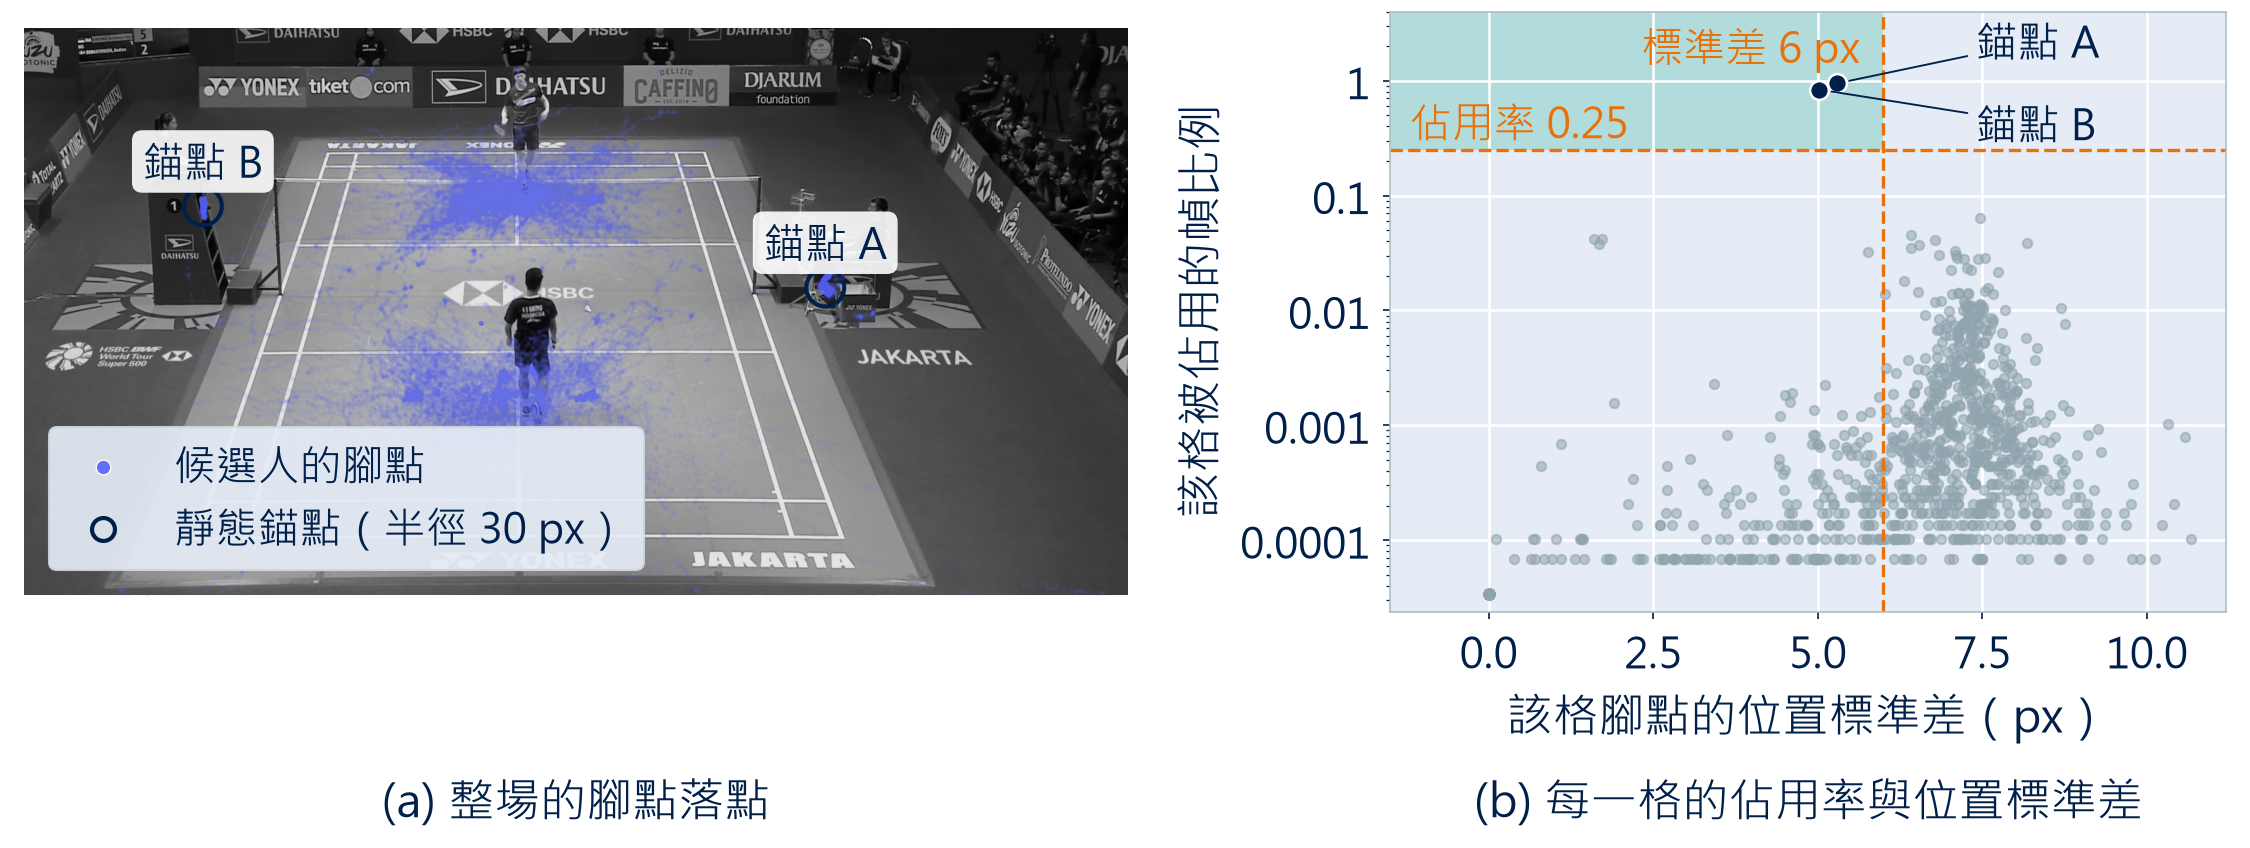
\includegraphics[width=\linewidth]{pose/static_anchors.png}
  \caption{整場腳點落點，固定不動者被判為靜態錨點}
  \label{fig:static-anchors}
\end{figure}

\textbf{有記憶的連續追蹤：}逐幀獨立選人仍會偶爾跳錯人，故改用帶短期記憶的追蹤器，有記憶時選離「上一幀所在位置」最近的人。記憶過舊即作廢，下一幀重新起始時無前一位置可依靠，便退回用公尺身高挑最高者。連續性成為依據，把漏偵時誤選裁判的風險壓到最低。

\section{球體分析}
\label{sec:shuttle-analysis}

\subsection{球體追蹤與軌跡重建}
\label{sec:shuttle-tracking}

\subsubsection{概述}

\textbf{問題與目標：}本模組為每個固定機位比賽片段重建羽球在畫面中的逐幀位置，作為下游擊球時刻偵測與球種分類的基礎。難點在於目標小、速度快，且球常被球員、球拍與球網遮擋。

\textbf{設計重點：}本模組沿用預訓練的 TrackNetV3，並利用時間連續性與運動約束，改善單幀偵測的誤判與缺失，主要有兩點做法：

\begin{enumerate}
  \item \textbf{多候選軌跡搜尋：}以低門檻保留每幀多個候選，再用 Viterbi 找出整段最連貫的路徑，使微弱但連續的真球能排除高信心的孤立誤偵。
  \item \textbf{互補雙軌跡：}同時輸出覆蓋率較高的 InpaintNet 軌跡與較保守的 Viterbi 軌跡，供下游依任務分工使用。
\end{enumerate}

\textbf{處理流程總覽：}如\figref{fig:shuttle-tracking-flow}。

\begin{figure}[H]
  \centering
  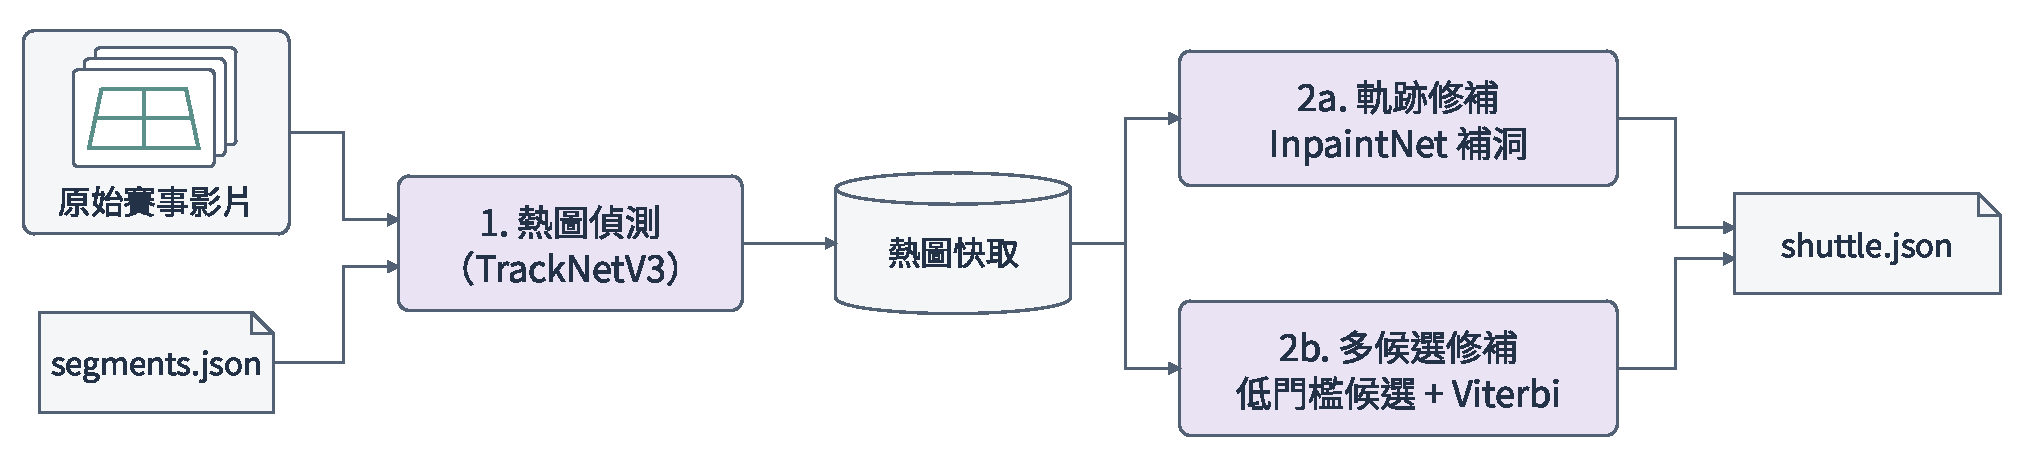
\includegraphics[scale=\flowscale]{shuttle-tracking.pdf}
  \caption{球體追蹤與軌跡重建處理流程}
  \label{fig:shuttle-tracking-flow}
\end{figure}

\subsubsection{熱圖偵測與快取}

第一階段要在極小又易與背景混淆的目標上給出可靠證據。系統使用 TrackNetV3 對連續影格進行推論，產生逐幀信心熱圖。熱圖能保留多個可能位置，使後續方法可利用時間連續性決定最合理的軌跡。由於熱圖推論是主要的 GPU 運算，系統將結果按片段快取，使 InpaintNet 與 Viterbi 能共用相同的偵測結果，並可在不重新推論的情況下反覆調整軌跡重建方法。

先以 largest-blob 讀出一條基準軌跡，用信心門檻二值化後取面積最大的連通區塊，以其中心為位置、區塊峰值為該幀信心（\figref{fig:heatmap-readout}）。這條基準軌跡是修補法的輸入，而選擇法另從同一份熱圖以低門檻自取候選。

\begin{figure}[H]
  \centering
  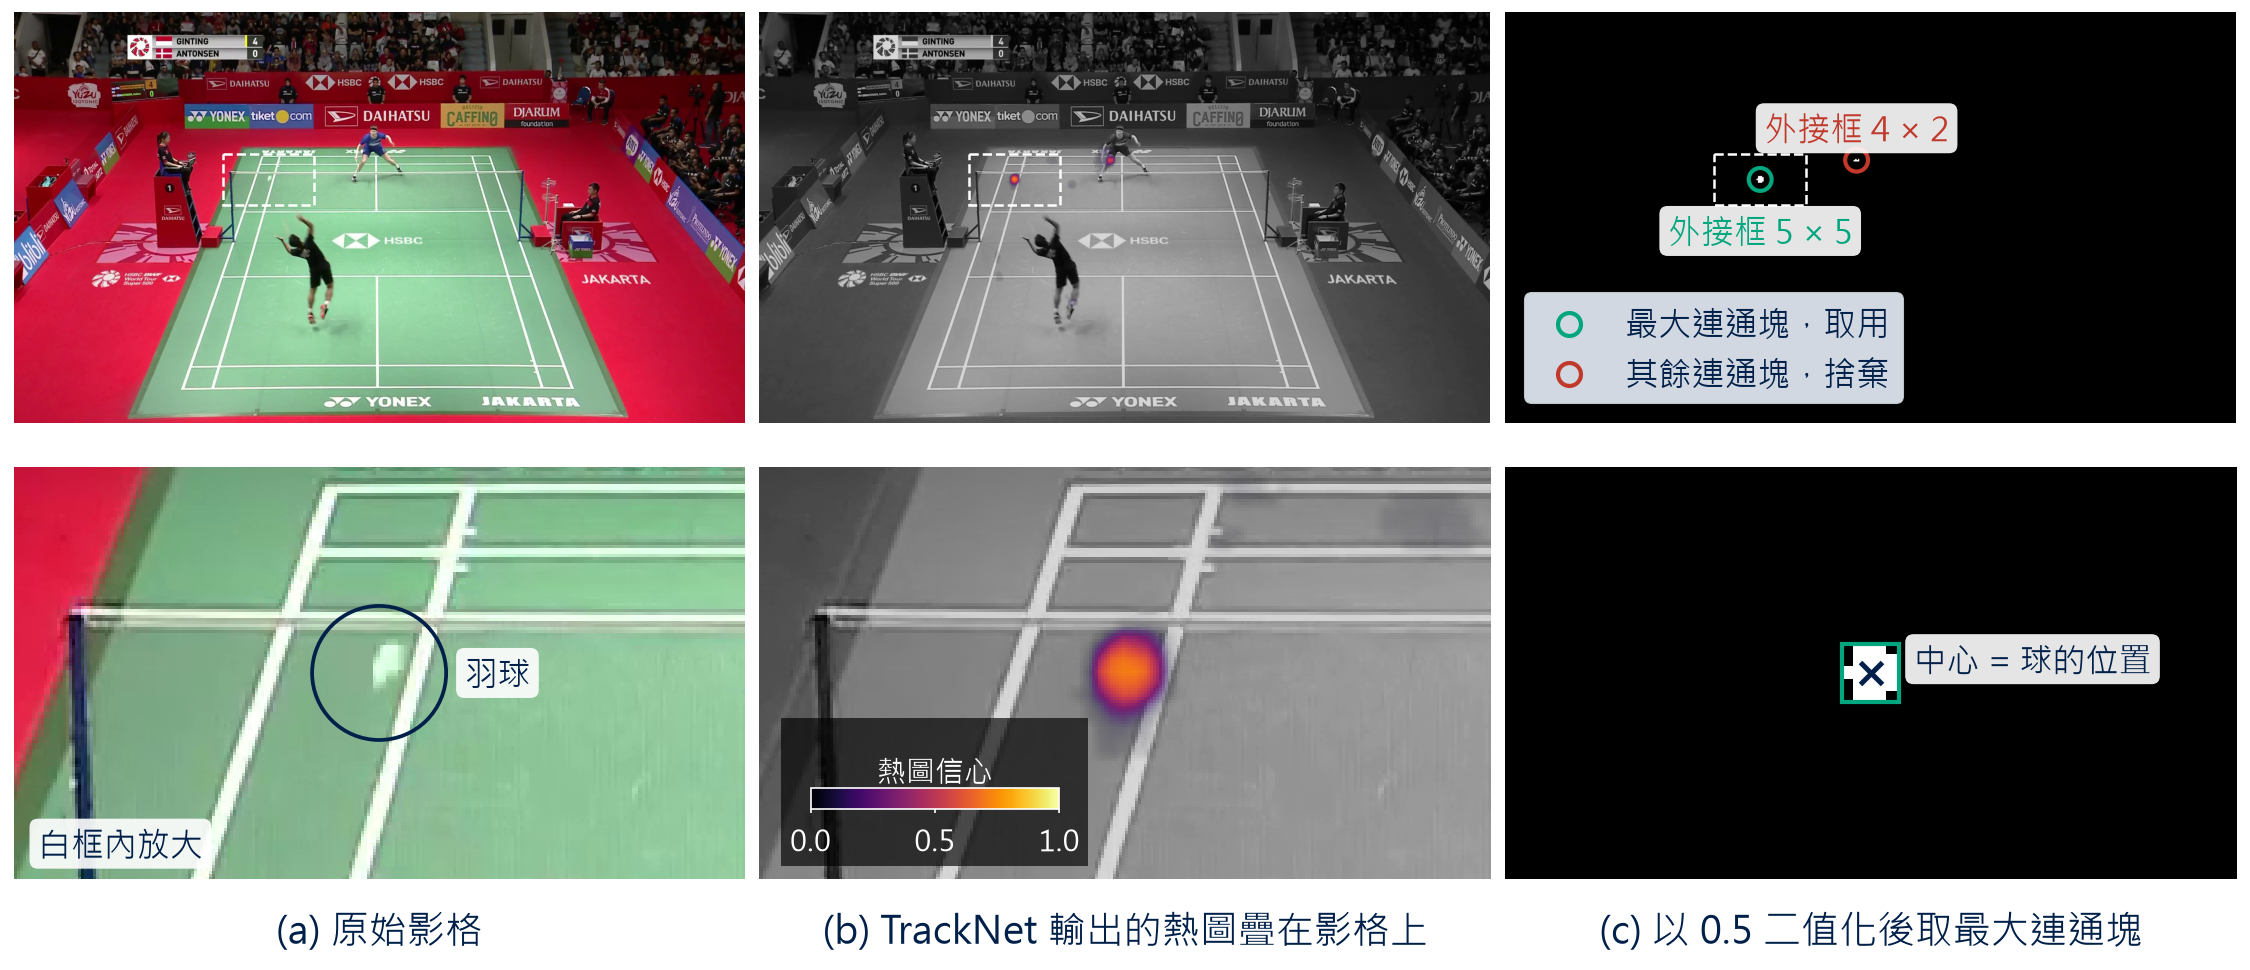
\includegraphics[width=\linewidth]{shuttle_tracking/heatmap_readout.png}
  \caption{從熱圖以 largest-blob 讀出基準軌跡}
  \label{fig:heatmap-readout}
\end{figure}

\subsubsection{軌跡修補（InpaintNet）}

第一種方法先將熱圖二值化，取每幀面積最大的連通區塊作為基準位置，再由補洞網路（InpaintNet~\cite{tracknetv3}）補回遮擋造成的缺幀（\figref{fig:inpaint-gaps}）。補值點的信心標為 0，使下游能區分實際偵測與模型推論。

\begin{figure}[H]
  \centering
  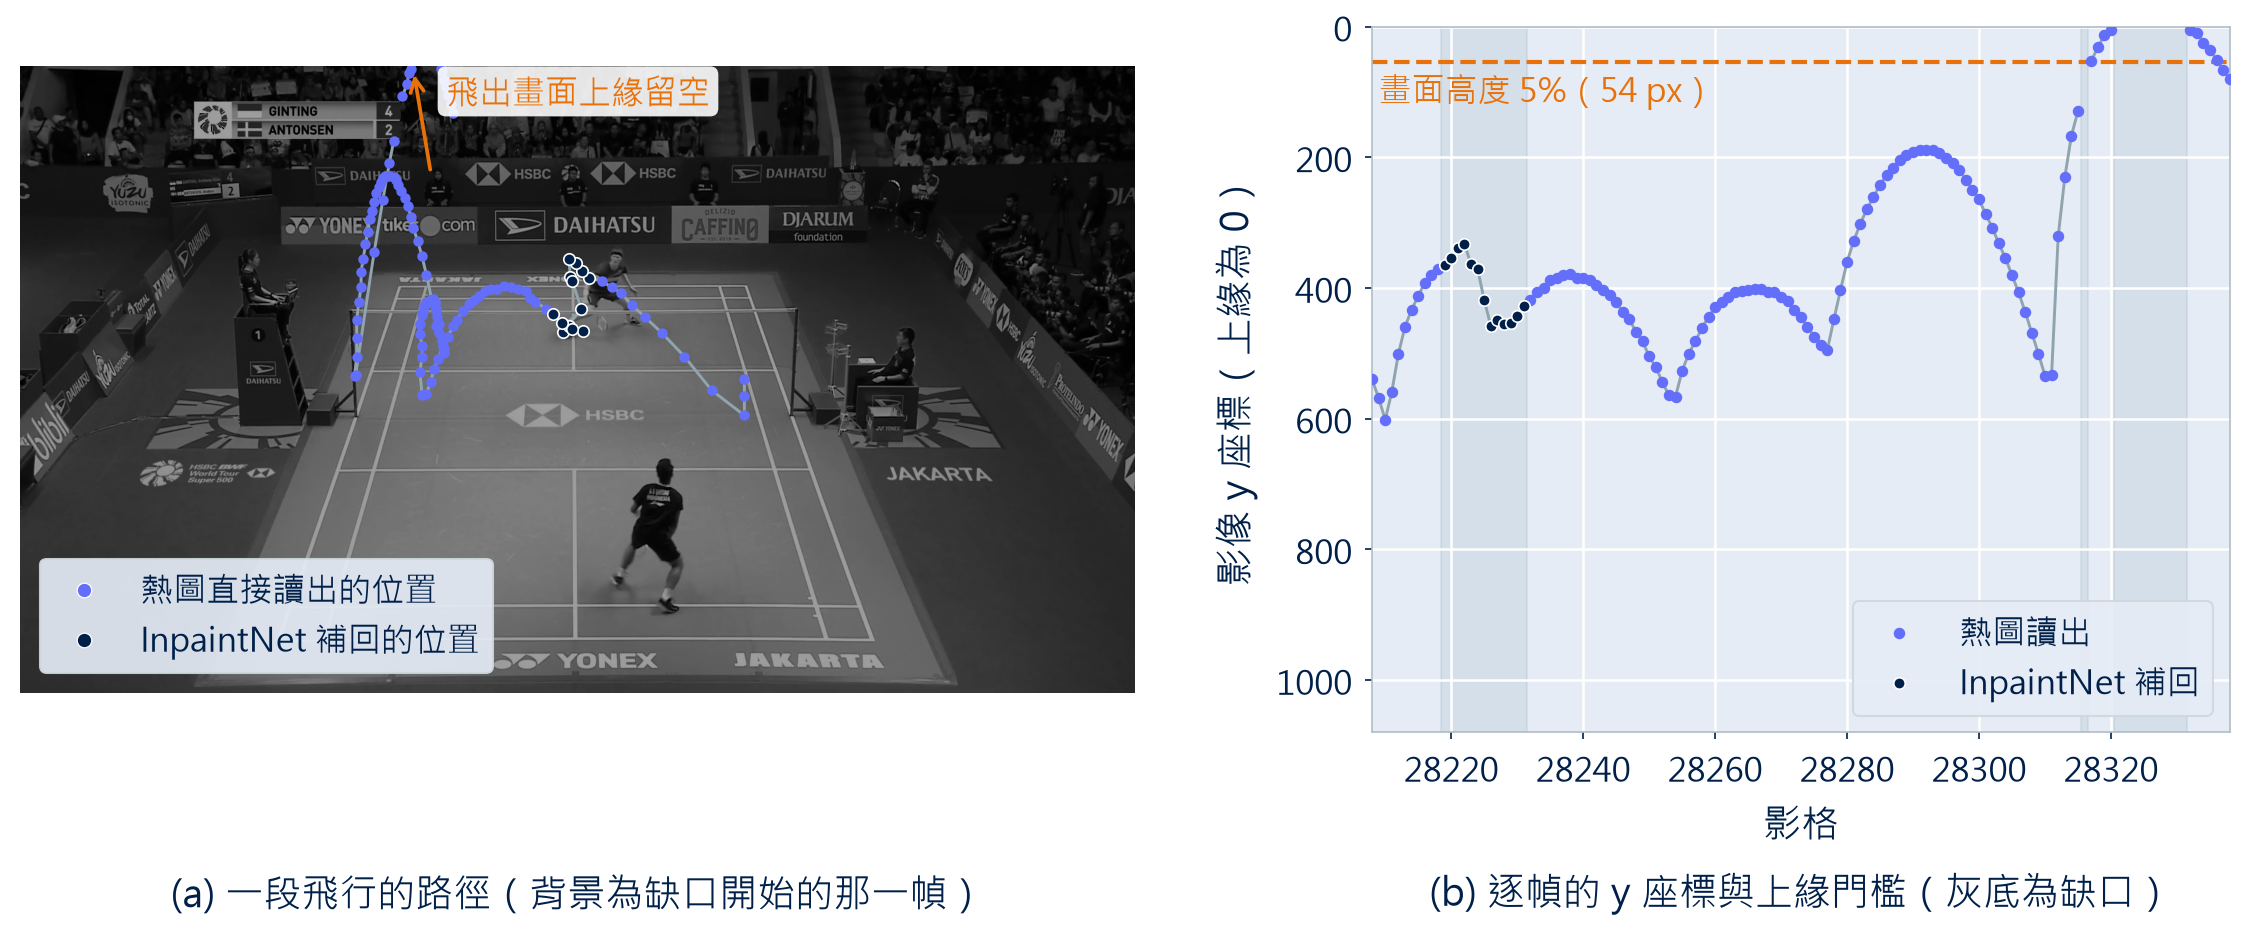
\includegraphics[width=\linewidth]{shuttle_tracking/inpaint_gaps.png}
  \caption{InpaintNet 補回球員遮擋造成的缺幀}
  \label{fig:inpaint-gaps}
\end{figure}

\subsubsection{多候選軌跡修補（Viterbi）}

第二種方法改以全域路徑搜尋壓制孤立誤偵。它用極低門檻把每幀所有稍可能是球的區塊全留作候選，再找一條最像真實飛行的路徑穿過它們。把每幀候選當節點、相鄰候選間連邊，給節點獎勵（信心越高越好）、給邊代價（前後兩點推出的速度越不合物理越貴、跨幀越多越貴），以動態規劃取總分最高的路徑。如此微弱但連貫的偵測能勝過強烈但孤立的偵測（\figref{fig:viterbi-path}）。當某幀球員鞋子或場線在信心上壓過真球，只要接不上前後飛行就不會入選。最後才對剩餘缺口依長度與兩端運動狀態決定補或不補，並以卡爾曼濾波填值。

\begin{figure}[H]
  \centering
  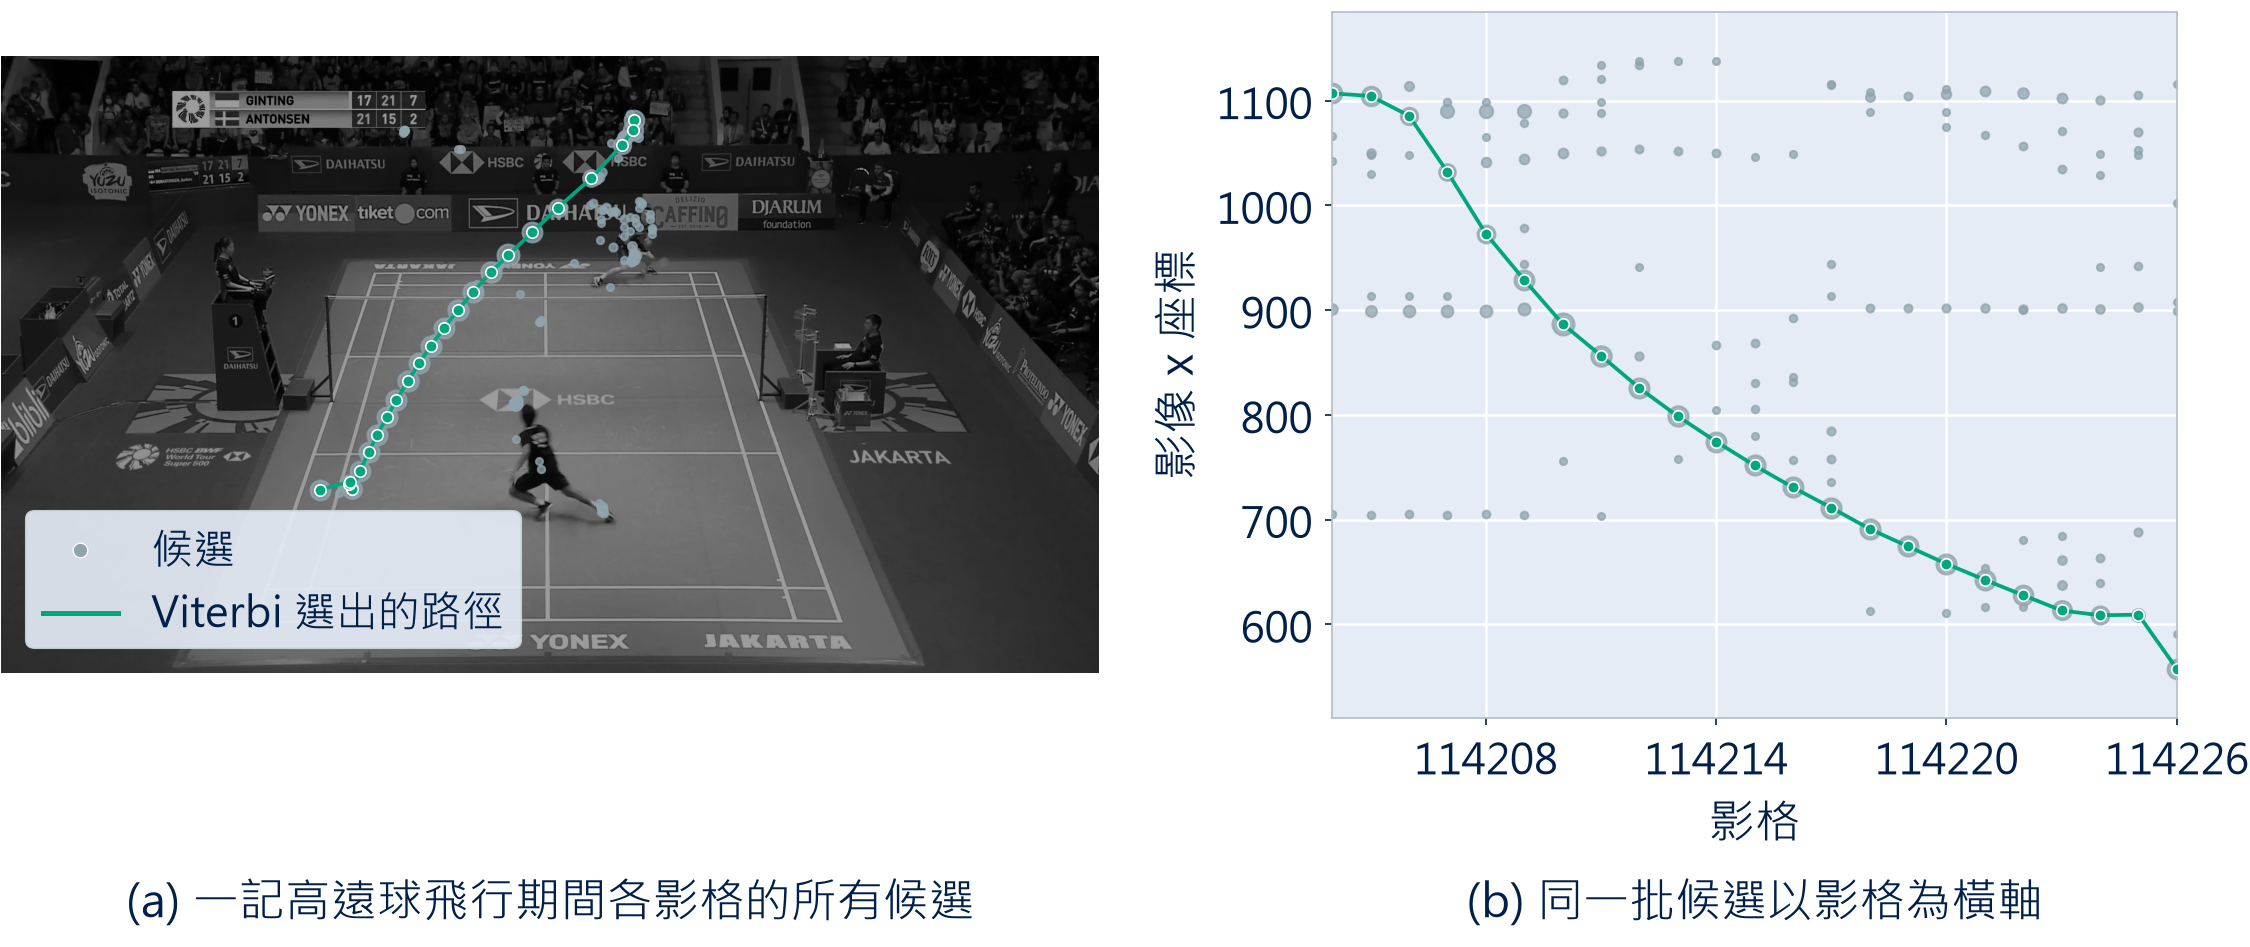
\includegraphics[width=\linewidth]{shuttle_tracking/viterbi_path.png}
  \caption{低門檻多候選與 Viterbi 選出的最佳路徑}
  \label{fig:viterbi-path}
\end{figure}

\subsubsection{雙軌跡並存}

修補法與選擇法各有所長、在不同情境下互有勝負，模組因此不在內部挑出贏家，而是把兩條軌跡都算出、都寫進 \texttt{shuttle.json}，把選擇交給握有更多上下文的下游。

\subsection{擊球時刻偵測}
\label{sec:hit-detection}

\subsubsection{概述}

\textbf{問題與目標：}本模組在每個片段內標記出每一擊球的影格，為下游球種分類提供窗口範圍。

\textbf{設計重點：}本模組的初始版本參考了開源專案 SoloShuttlePose 的擊球事件偵測（\texttt{event\_detect}）~\cite{soloshuttlepose}，其僅以單條球體軌跡的 Y 軸峰值與軌跡轉角判定擊球。現行版本在其基礎上重新設計，改以多源證據融合與結構性補漏取代單一軌跡幾何。一次擊球是軌跡上一瞬間的事件，只在球路上留下細微痕跡，任何單一訊號都不夠可靠。本模組因此同時融合多種訊號，並以召回優先，把不漏拍作為首要目標。主要有兩點做法：

\begin{enumerate}
  \item \textbf{多源證據融合：}不押注單一訊號，同時利用兩條球體軌跡、球員骨架與逐幀球種模型三種來源。相對於只讀軌跡幾何的做法，任一來源在特定情境失效時仍能由其他來源補上。
  \item \textbf{結構性補洞：}不靠放寬偵測門檻加球，而是從「結構上一定有一拍」的位置（交替違規、模型長時間鎖定、發球遮擋）反推漏拍位置。
\end{enumerate}

在 8 場未參與開發的比賽上，本模組在 $\pm$5 影格容差下召回率 90.90\%、精確率 95.49\%（見\secref{sec:exp-events}）。

\textbf{處理流程總覽：}如\figref{fig:event-detection-flow}。

\begin{figure}[H]
  \centering
  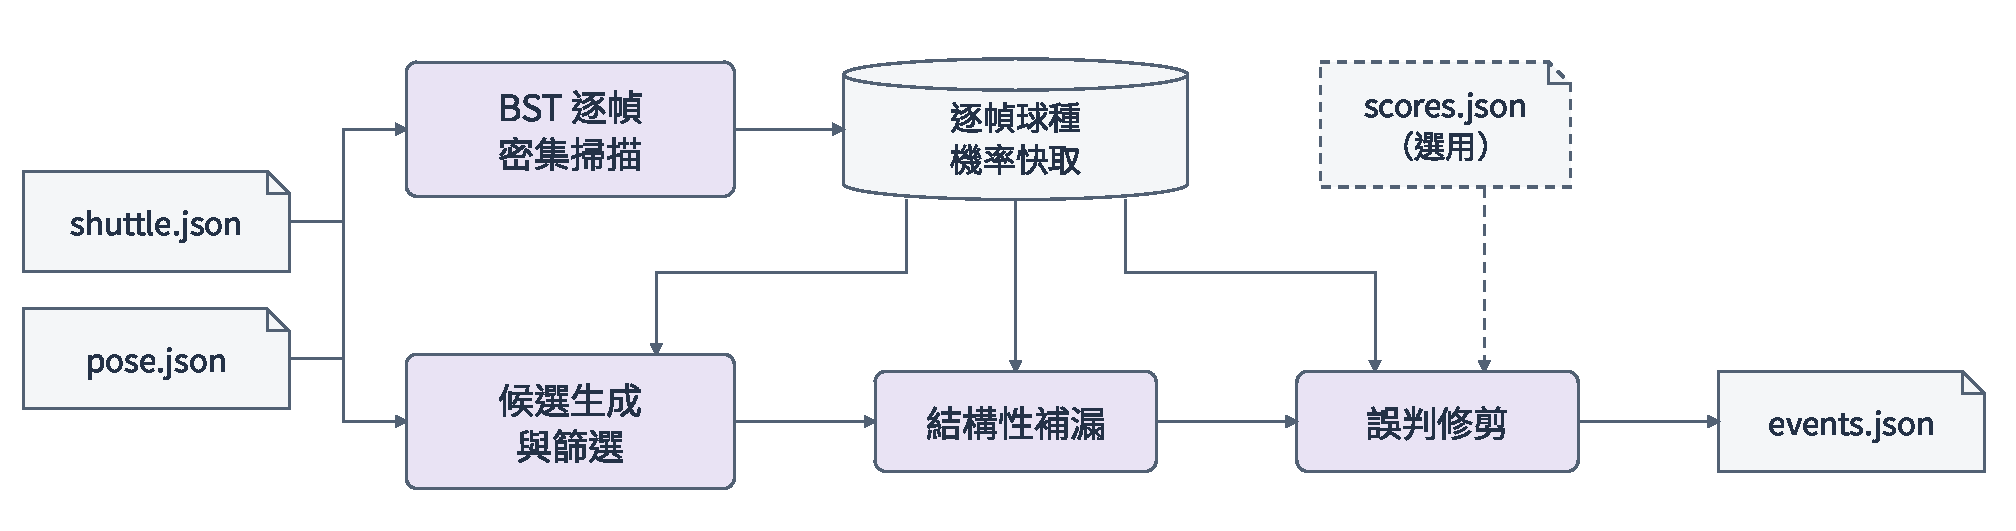
\includegraphics[scale=\flowscale]{event-detection.pdf}
  \caption{擊球時刻偵測處理流程}
  \label{fig:event-detection-flow}
\end{figure}

\subsubsection{逐幀球種證據}

本模組先對每個片段逐影格掃描，將每個影格前後各半秒的窗口，輸入球種分類模型 BST~\cite{bst}，得到該影格的 25 類球種機率分布。

BST 原本設計的窗口是「兩次擊球之間」，需要以擊球時刻作為窗口邊界。但在本模組，擊球時刻正是需要偵測的目標。因此本模組將所有影格以固定窗口輸入模型，並將輸出反過來作為是否存在擊球的判斷依據之一。BST 的輸出提供三種輔助證據（\figref{fig:dense-evidence}）：

\textbf{球種信心：}若模型對某個影格的窗口給出高信心的球種判斷（例如 0.9 的殺球），代表這個窗口的球路與骨架很接近某個真實擊球的樣態。相較於另一個最高信心僅 0.3 的窗口，前者更可能對應到一次真實擊球。

\textbf{擊球者判定：}即使窗口沒對齊擊球，模型對「擊球者位於畫面上方或下方」的判斷仍相當可靠，比單純比較羽球與兩名球員的距離更為準確，因此在後續分邊時作為優先證據。

\textbf{連續球種區間：}若把某個真實擊球影格前後半秒作為窗口輸入模型會得到球種 a，那麼對它鄰近的前後一兩影格做同樣的事，因窗口內容高度重疊，也極可能得到相同的球種 a，只是信心略低。反過來說，只要觀察到連續多個窗口被判為同一球種，就代表該區間附近很可能存在一次擊球。

\begin{figure}[H]
  \centering
  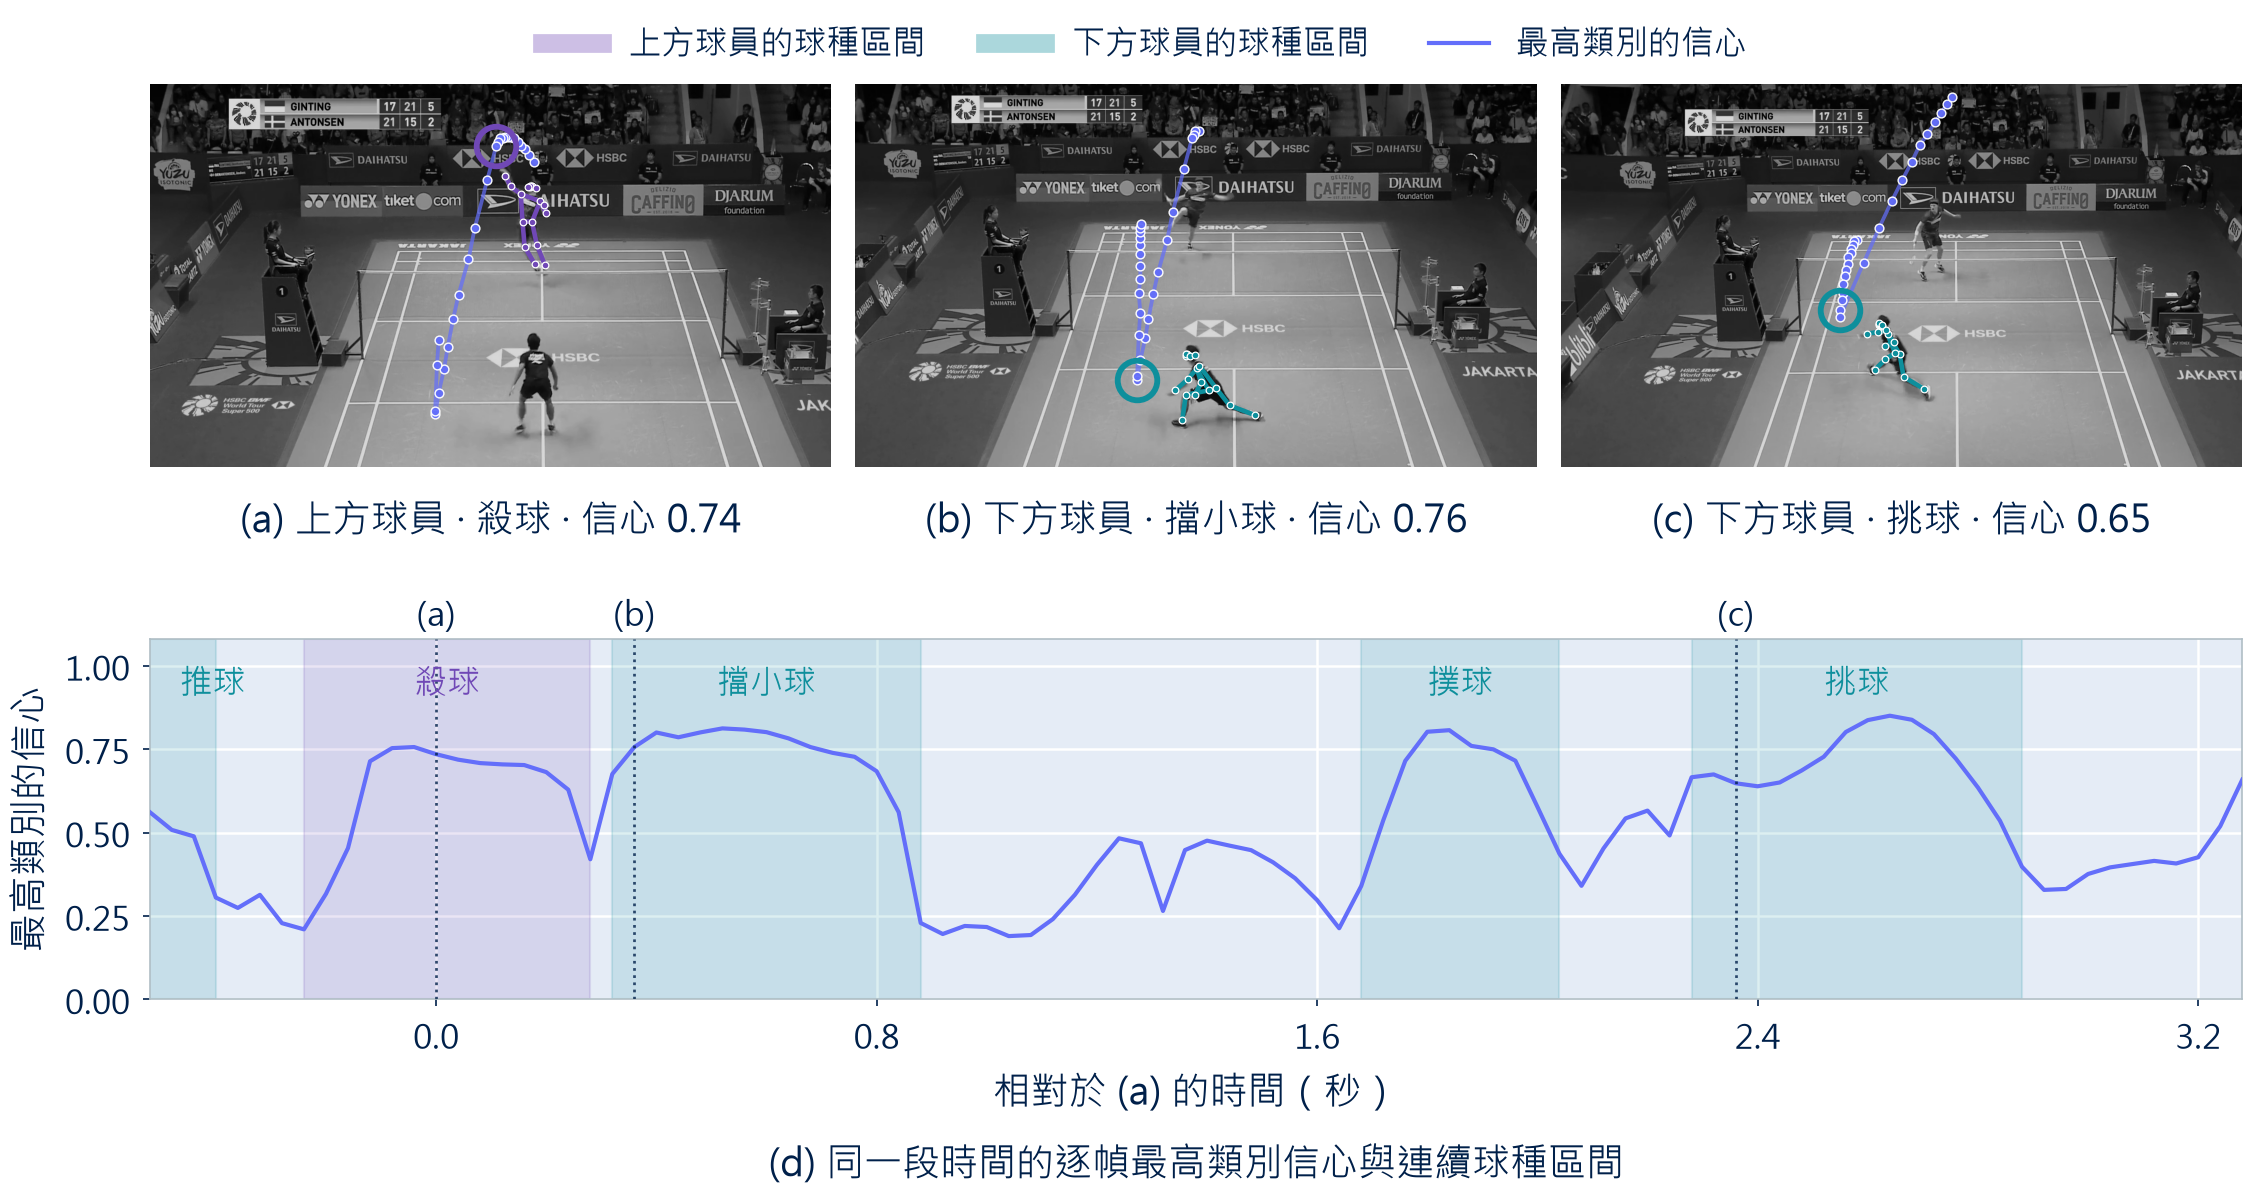
\includegraphics[width=\linewidth]{event_detection/dense_evidence.png}
  \caption{逐幀滑動窗口產生的球種、信心與擊球者證據}
  \label{fig:dense-evidence}
\end{figure}

\subsubsection{候選生成}

本步驟分析軌跡中實際存在的有效點。由於不同球種在軌跡上的差異很大，不同位置擊球也會造成軌跡產生不同變化，因此單一訊號無法抓出所有擊球。本步驟尋找下列互補的擊球特徵（\figref{fig:candidate-signals}）：

\textbf{垂直轉折：}影像座標的 $y$ 值向下增加，因此羽球下降至球員附近、擊球後重新上升時，會在軌跡上形成局部最大值。

\textbf{方向與速率突變：}比較候選前後的速度向量，若方向明顯轉折且速率比例突然改變，較可能是球拍接觸，而非重力造成的平順轉彎。

\textbf{由慢轉快：}平抽或快速推球未必形成明顯垂直轉折，因此另以擊球前後的速率比及水平速度變化尋找候選。

\textbf{發球錨點：}額外偵測回合開頭的陡峭垂直變化與第一段持續上升軌跡，作為發球候選。

本步驟刻意偏向敏感、高召回，先保留不確定候選，再交由後續規則排除（\figref{fig:candidate-pool}）。擊球時刻要用來為下一階段的球種模型切分析窗口，一旦漏掉一拍，窗口就會整段錯位，後續的比賽脈絡也會出現難以復原的斷點。

\begin{figure}[H]
  \centering
  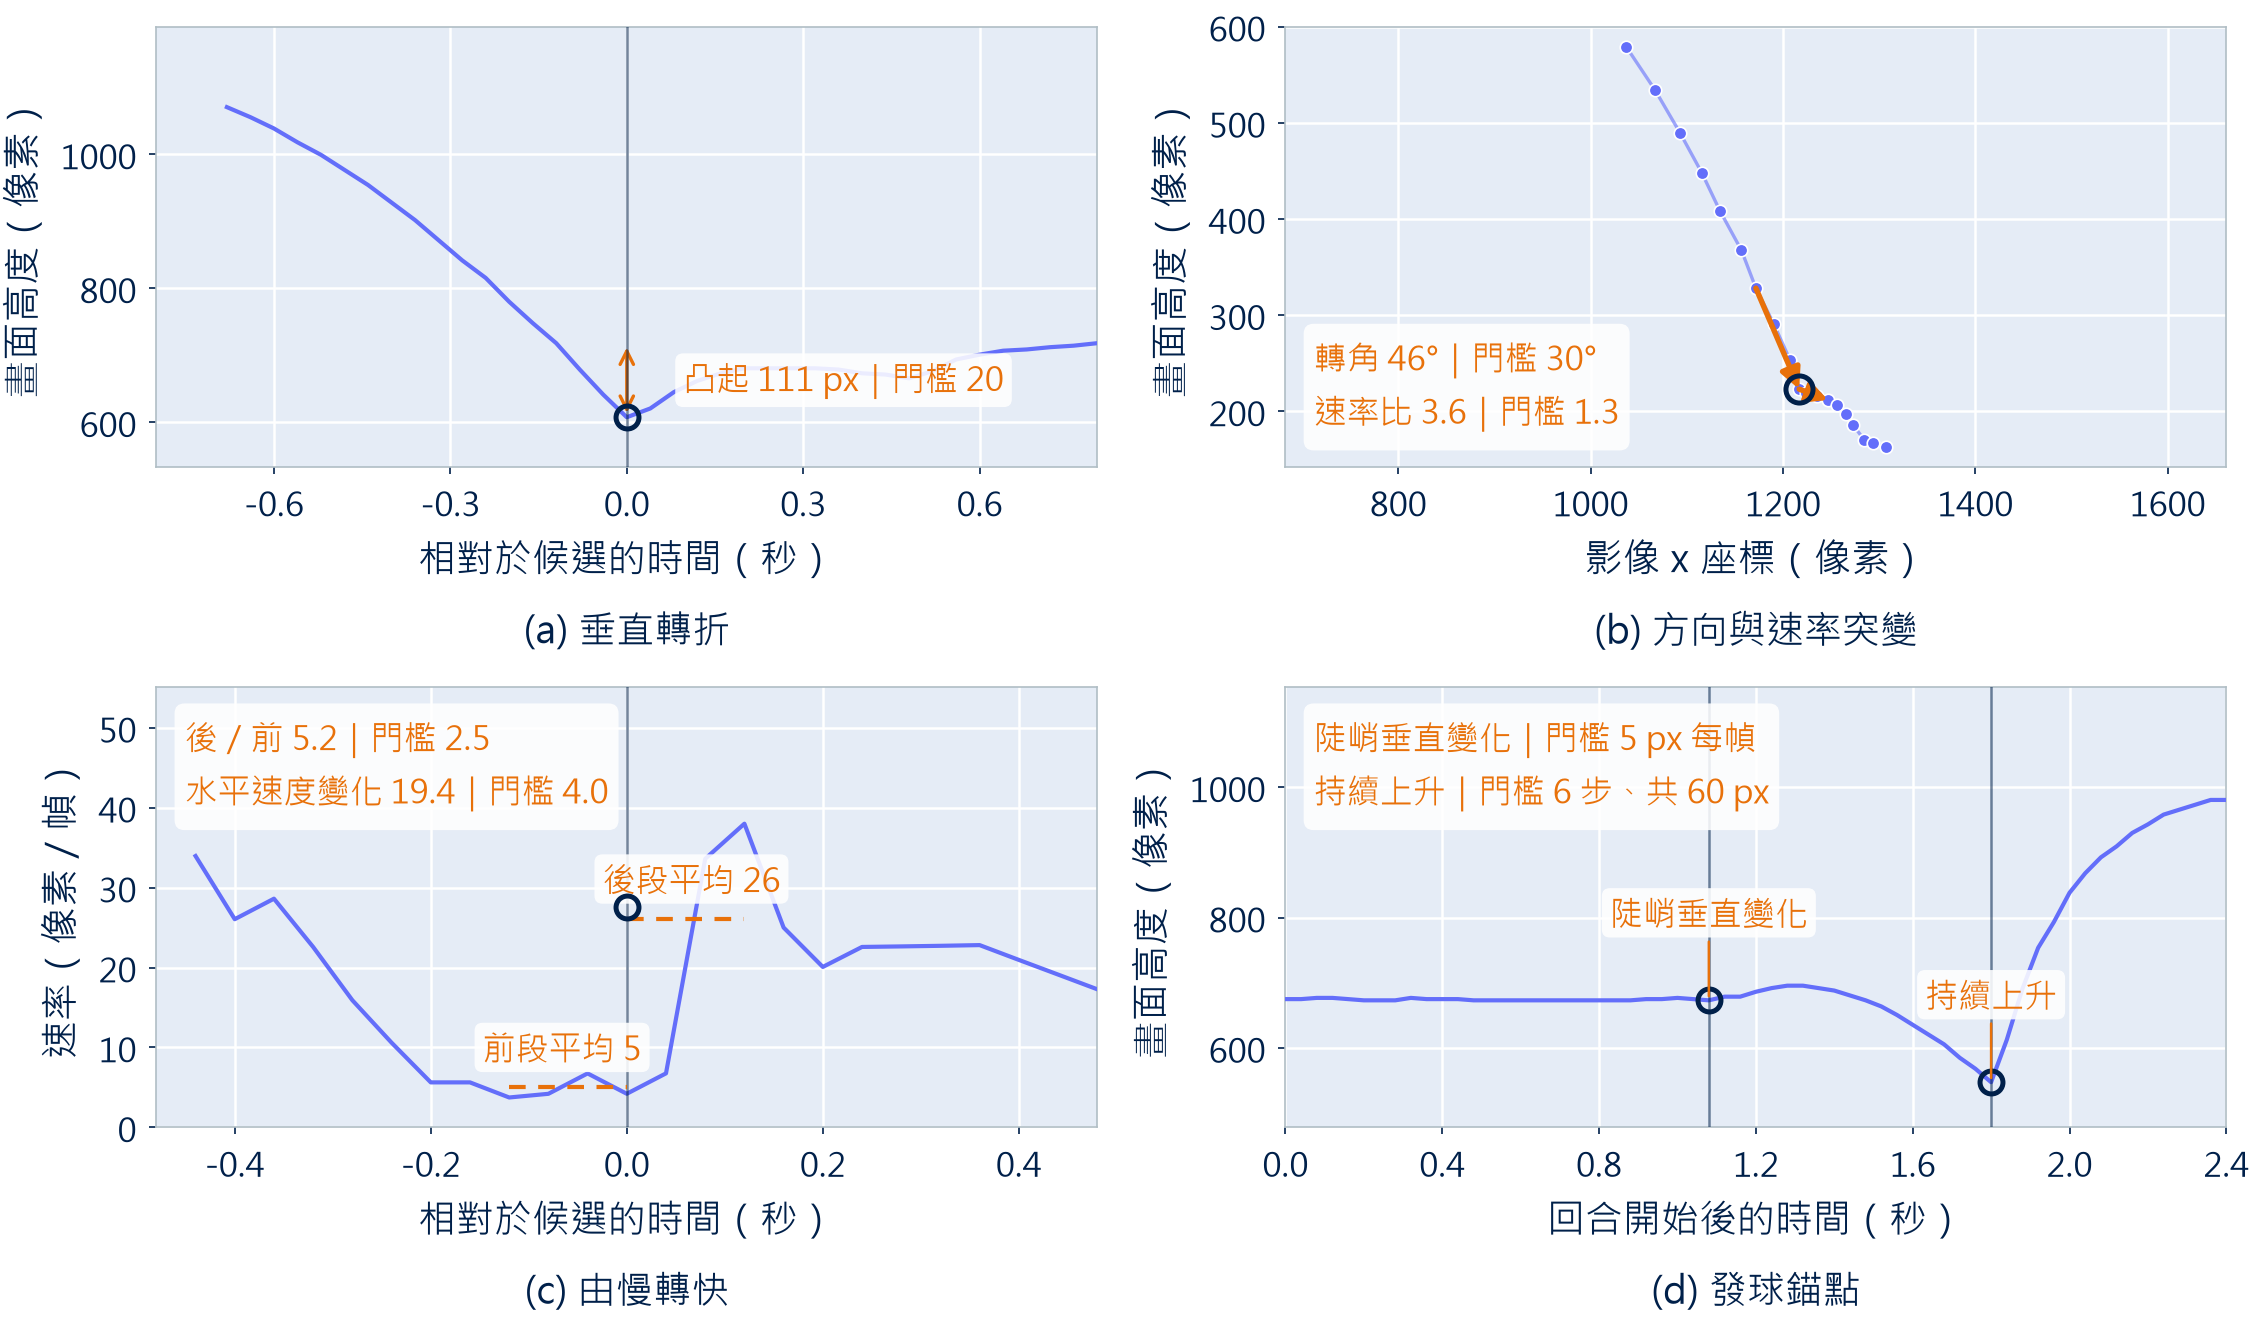
\includegraphics[width=\linewidth]{event_detection/candidate_signals.png}
  \caption{四種互補的擊球候選訊號}
  \label{fig:candidate-signals}
\end{figure}

\begin{figure}[H]
  \centering
  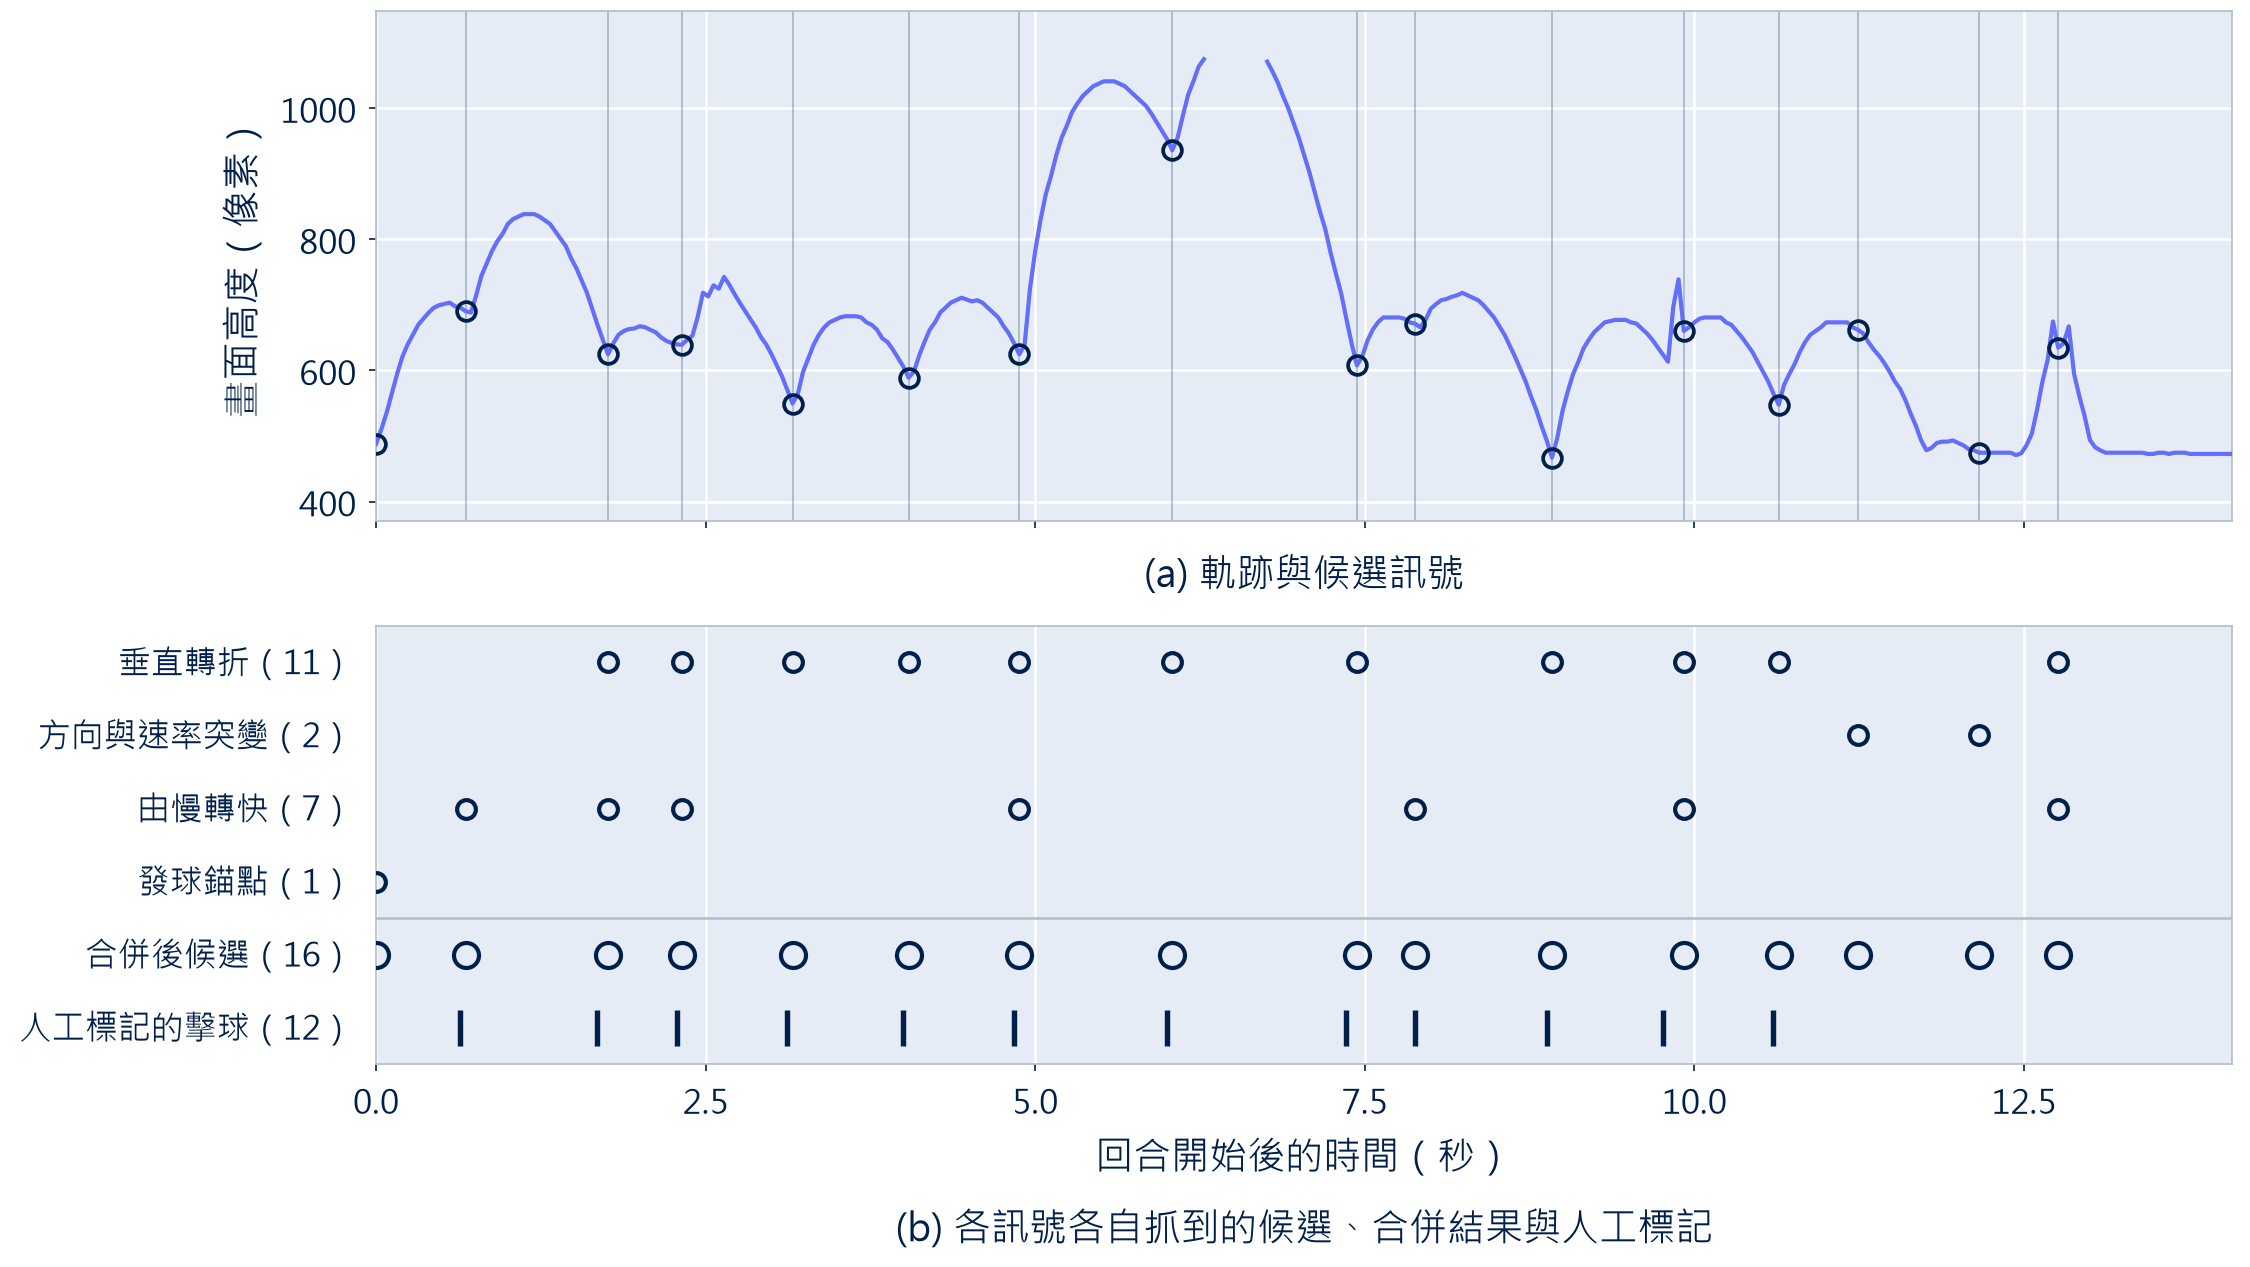
\includegraphics[width=\linewidth]{event_detection/candidate_pool.png}
  \caption{各訊號在完整回合中的候選分布與合併結果}
  \label{fig:candidate-pool}
\end{figure}

\subsubsection{候選篩選}

本步驟將候選經過三道篩選（\figref{fig:candidate-gates}）：

\textbf{位移振幅：}計算候選附近時間窗內的水平與垂直位移範圍，只要其中一軸具有足夠位移便予以保留，以排除球落地後的微小追蹤抖動。

\textbf{同球員去重：}依靠 BST 的輸出判定擊球者，若時間相近的連續候選被判為同球員擊球，通常代表一次擊球同時觸發多種軌跡訊號。系統只保留水平與垂直位移振幅總和較大的候選。

\textbf{回合脈絡：}已知擊球側的候選附近應能找到對側球員的其他擊球候選。目前規則要求在指定時間窗內至少存在兩個對側候選，否則將其視為落地彈跳、追蹤脫線或其他孤立訊號。

\begin{figure}[H]
  \centering
  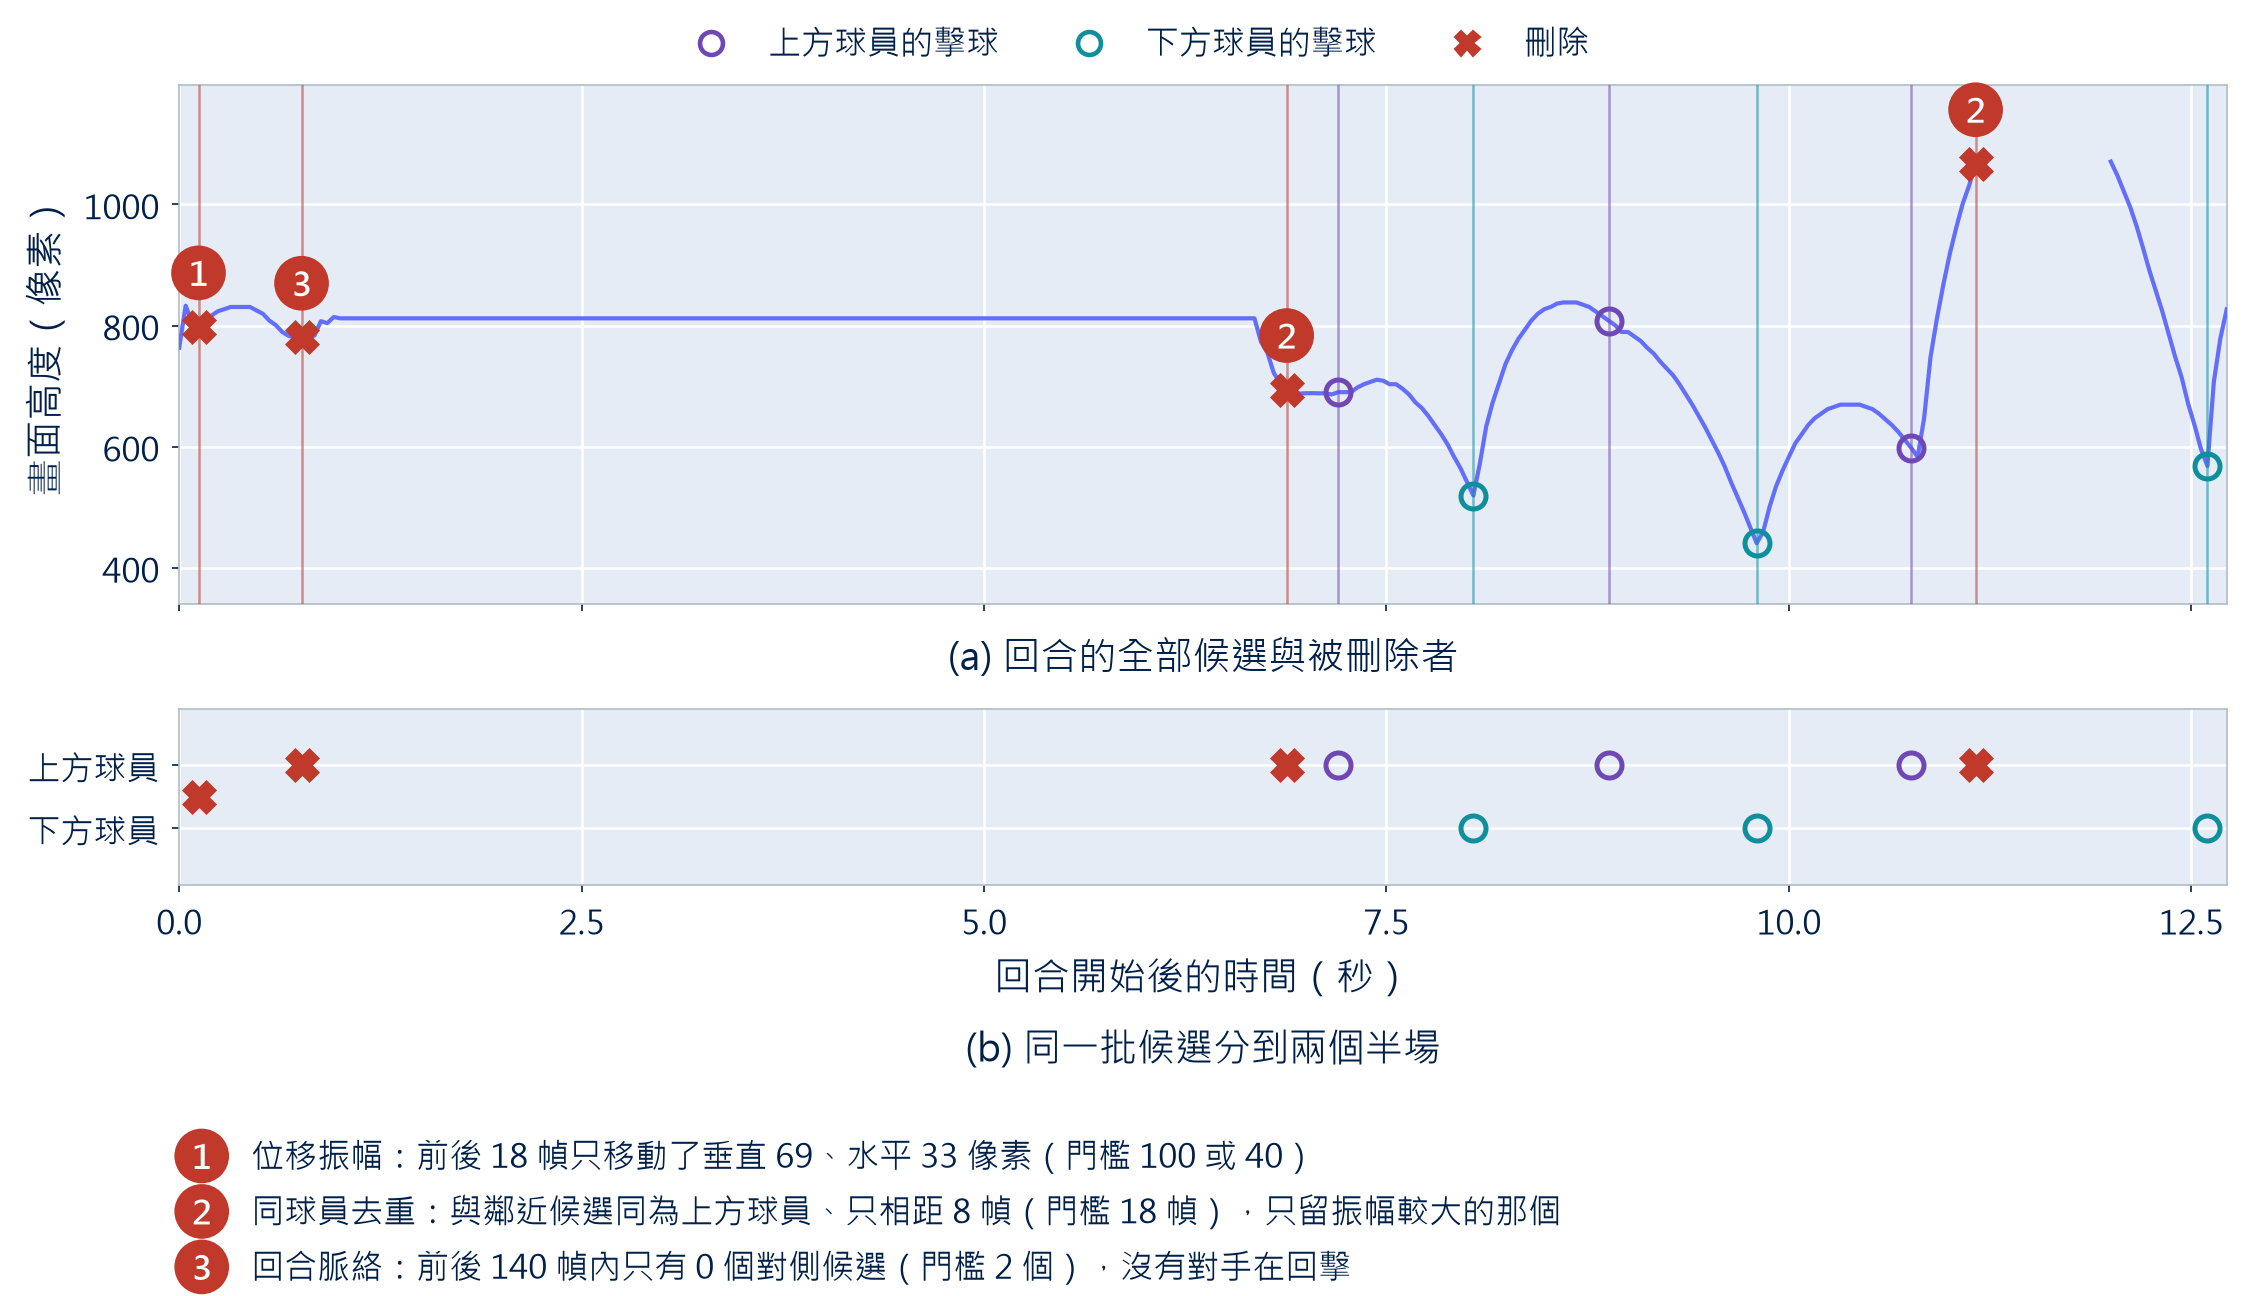
\includegraphics[width=\linewidth]{event_detection/candidate_gates.png}
  \caption{三道候選篩選規則及其保留／刪除結果}
  \label{fig:candidate-gates}
\end{figure}

\subsubsection{結構性補漏}

單靠放寬候選門檻會同時增加大量誤判，因此本步驟只在回合結構或多源證據顯示「此處很可能漏了一拍」時加入擊球。補漏刻意安排在候選篩選之後，序列先經篩選、去除雜訊後較為乾淨，回合脈絡才判斷得準，也才能據此救回一些訊號微弱、難以直接偵測的球。四條補漏規則依序執行，且新加入的擊球不得與既有擊球過近。

\textbf{交替違規補漏：}若序列中相鄰兩拍均由同球員擊出，代表兩者之間可能漏掉一拍對側擊球。系統依序搜尋主軌跡上較弱的垂直或水平轉折，以及 BST 的對側高信心連續區間，找到足夠證據後才補一拍。

\textbf{未被認領的鎖定區間：}若 BST 長時間、高信心地維持同一球種，但附近沒有任何擊球，系統會在該區間內尋找通過振幅條件的弱垂直轉折（\figref{fig:fill-sequence}）。BST 在此只指出可能漏拍的區域，不單獨決定擊球影格。

\textbf{輔助軌跡救援：}球體追蹤模組除了主軌跡，另輸出一條 Viterbi 軌跡（見\secref{sec:shuttle-tracking}），能看到主軌跡因遮擋或過度平滑而漏掉的球。若這條輔助軌跡在某處偵測到候選，且該候選接近 BST 球種訊號的起點、具有足夠信心，便將它加入。

\textbf{近端發球補漏：}畫面下方球員發球時，部分軌跡可能被身體遮擋。若持續上升錨點附近尚無擊球，而 BST 同時提供下方球員的發球證據，系統便在附近被篩掉的候選中選擇最接近者（\figref{fig:fill-trajectory}）。

\begin{figure}[H]
  \centering
  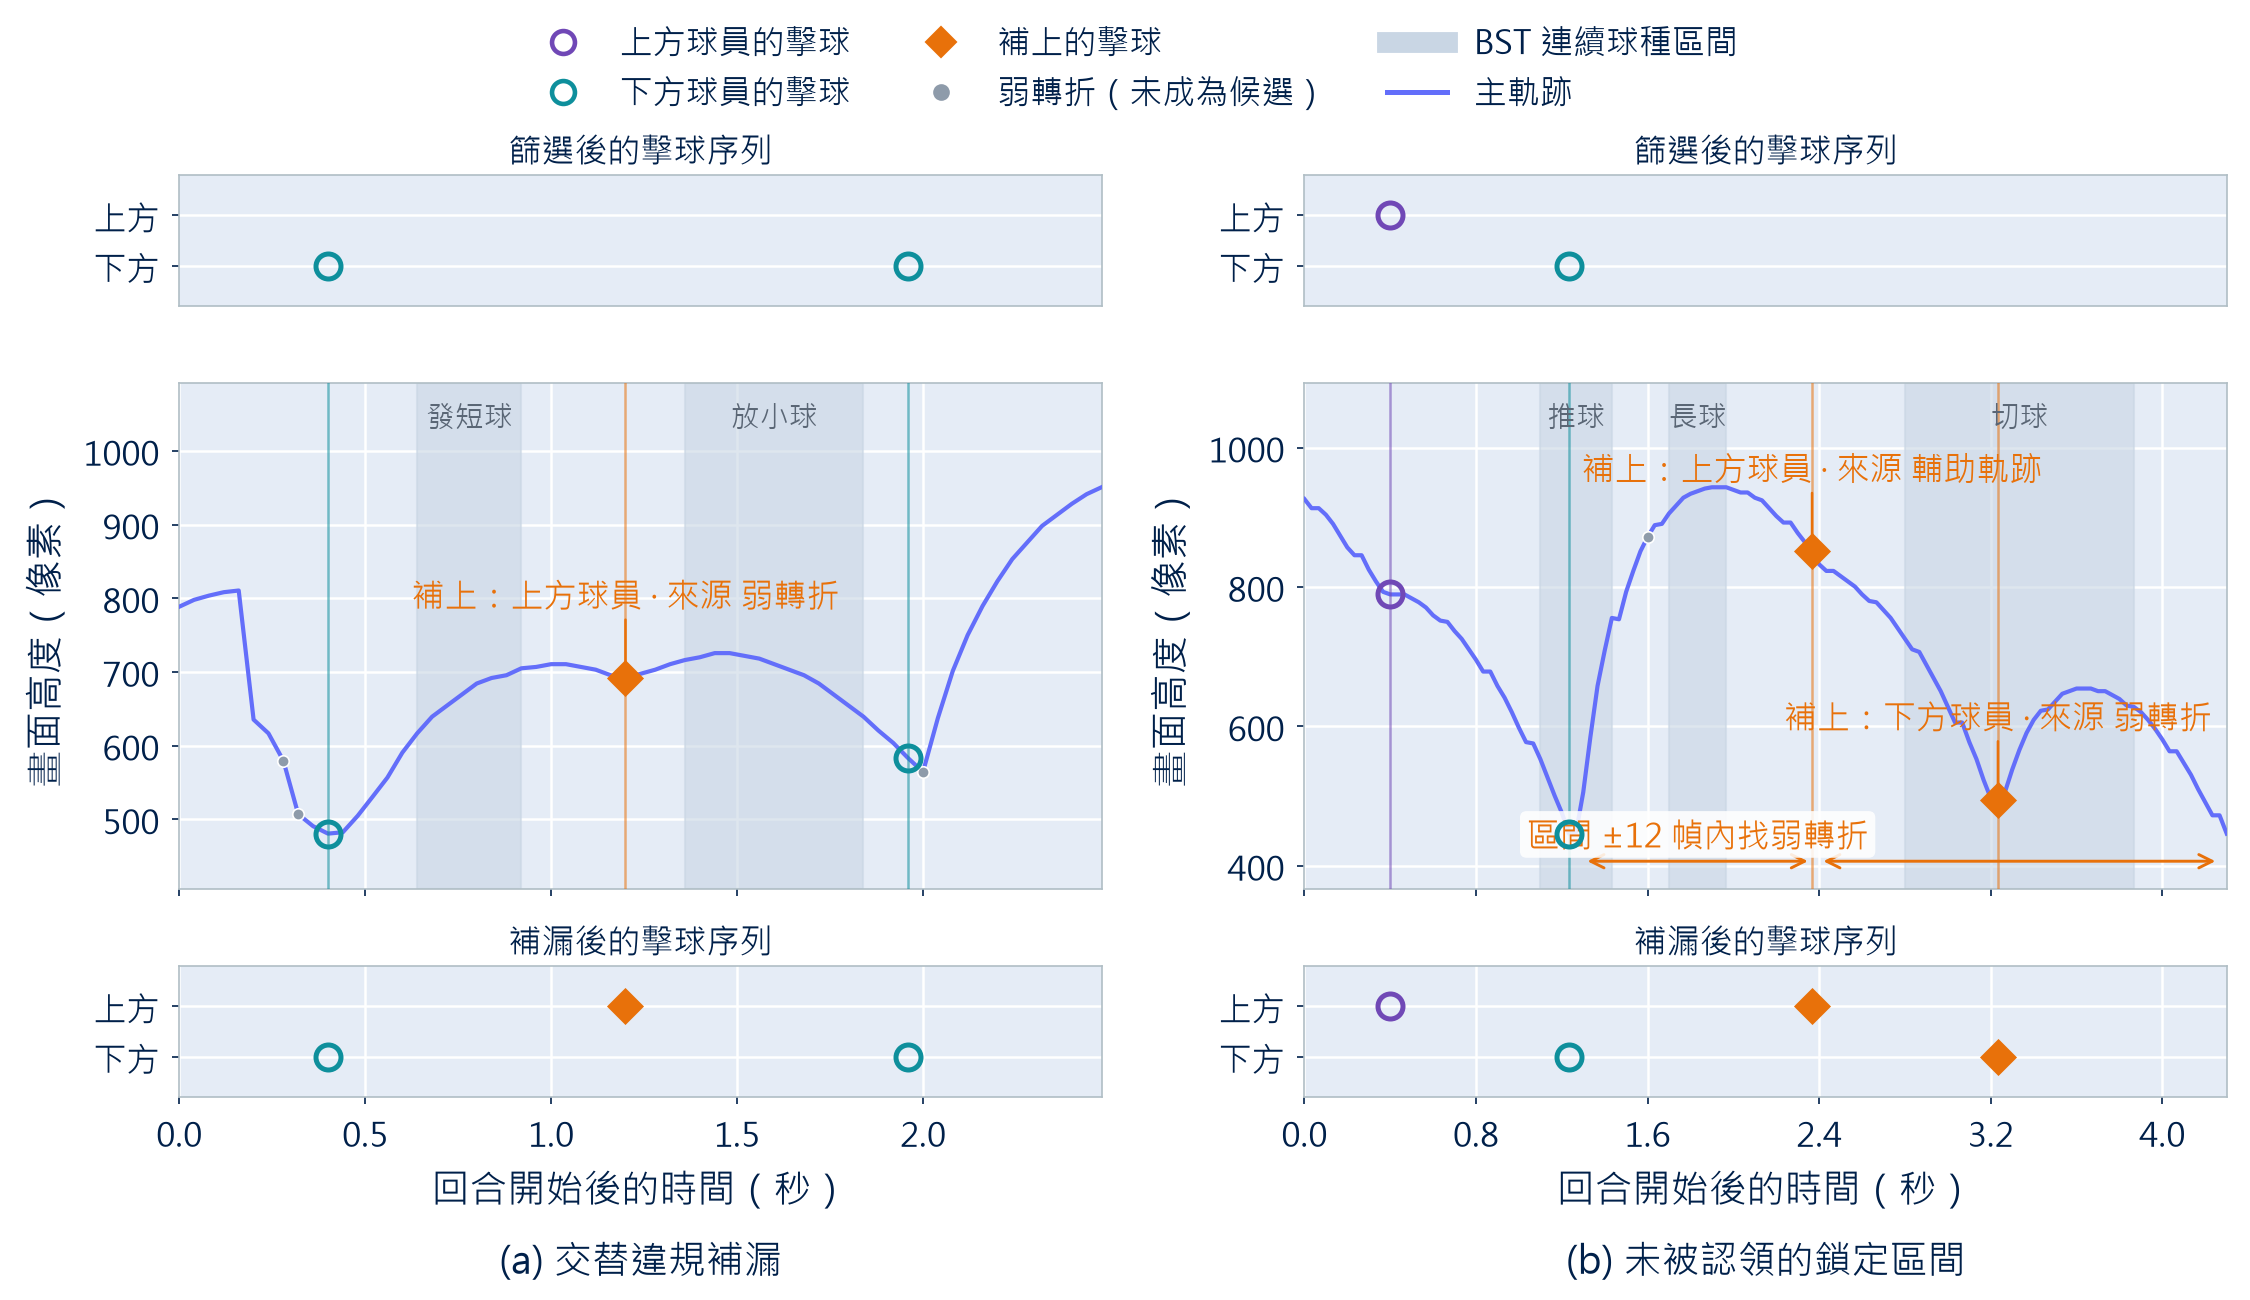
\includegraphics[width=\linewidth]{event_detection/fill_sequence.png}
  \caption{由擊球序列與連續球種證據反推漏拍位置}
  \label{fig:fill-sequence}
\end{figure}

\begin{figure}[H]
  \centering
  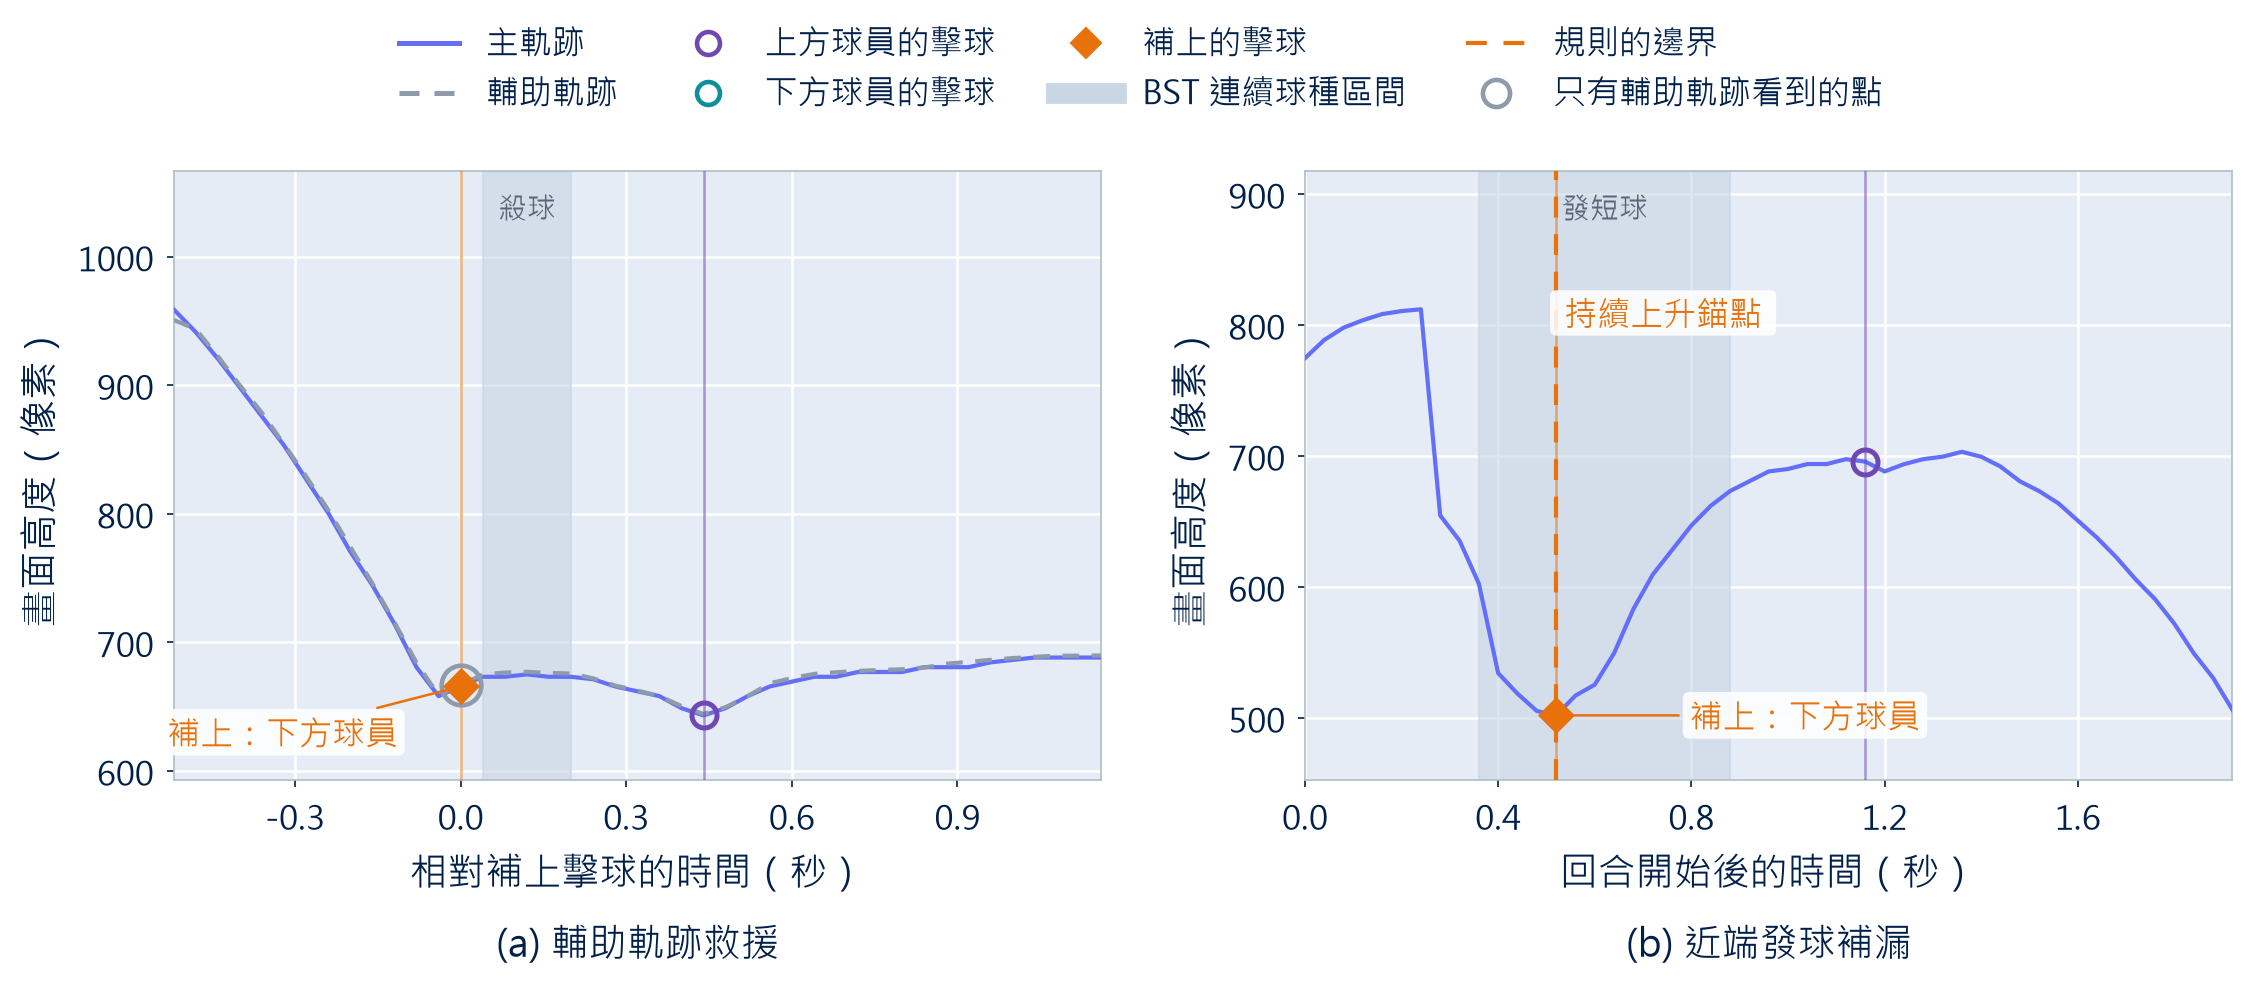
\includegraphics[width=\linewidth]{event_detection/fill_trajectory.png}
  \caption{由輔助軌跡與發球錨點救回漏拍}
  \label{fig:fill-trajectory}
\end{figure}

\subsubsection{誤判修剪}

本步驟清理回合邊緣不屬於實際對打的少數雜訊。僅針對三種很特定、平時不常觸發的情況：

\textbf{回合有效區間：}發球前場上還沒有球在移動，球體追蹤可能把反光亮點之類誤認成球，生出不存在的球路，需剔除。

\textbf{尾段落地球：}回合結束後，羽球的彈跳與滾動仍可能產生軌跡轉折，需剔除（\figref{fig:prune-rally-edges}）。

\textbf{計分板死時間：}特定休息比分下的計分板死時間（如開局 0:0、局中技術暫停，\figref{fig:prune-scoreboard}）。

\begin{figure}[H]
  \centering
  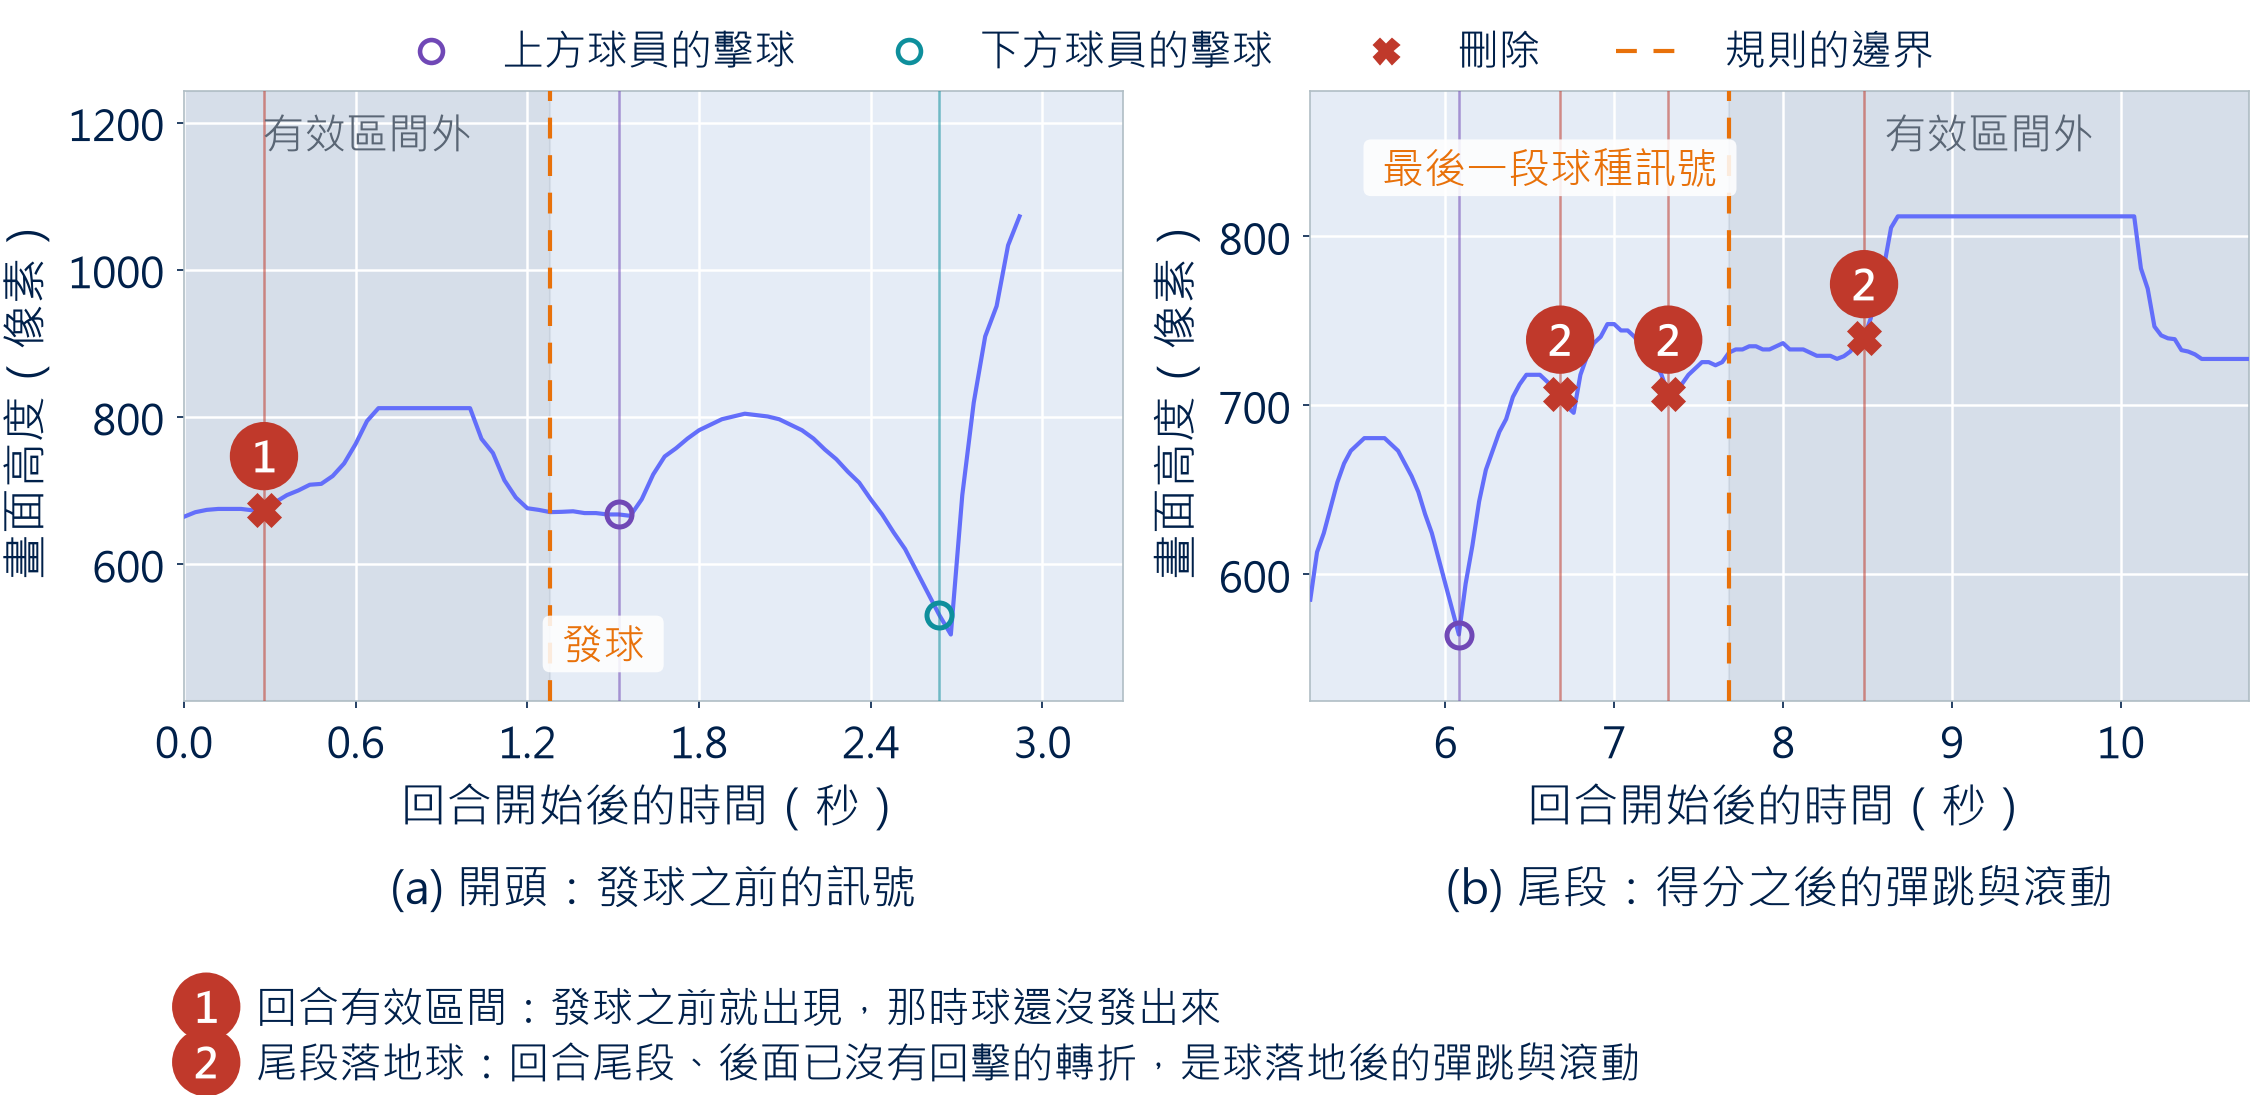
\includegraphics[width=\linewidth]{event_detection/prune_rally_edges.png}
  \caption{利用回合有效邊界清除開頭誤偵與尾段落地球}
  \label{fig:prune-rally-edges}
\end{figure}

\begin{figure}[H]
  \centering
  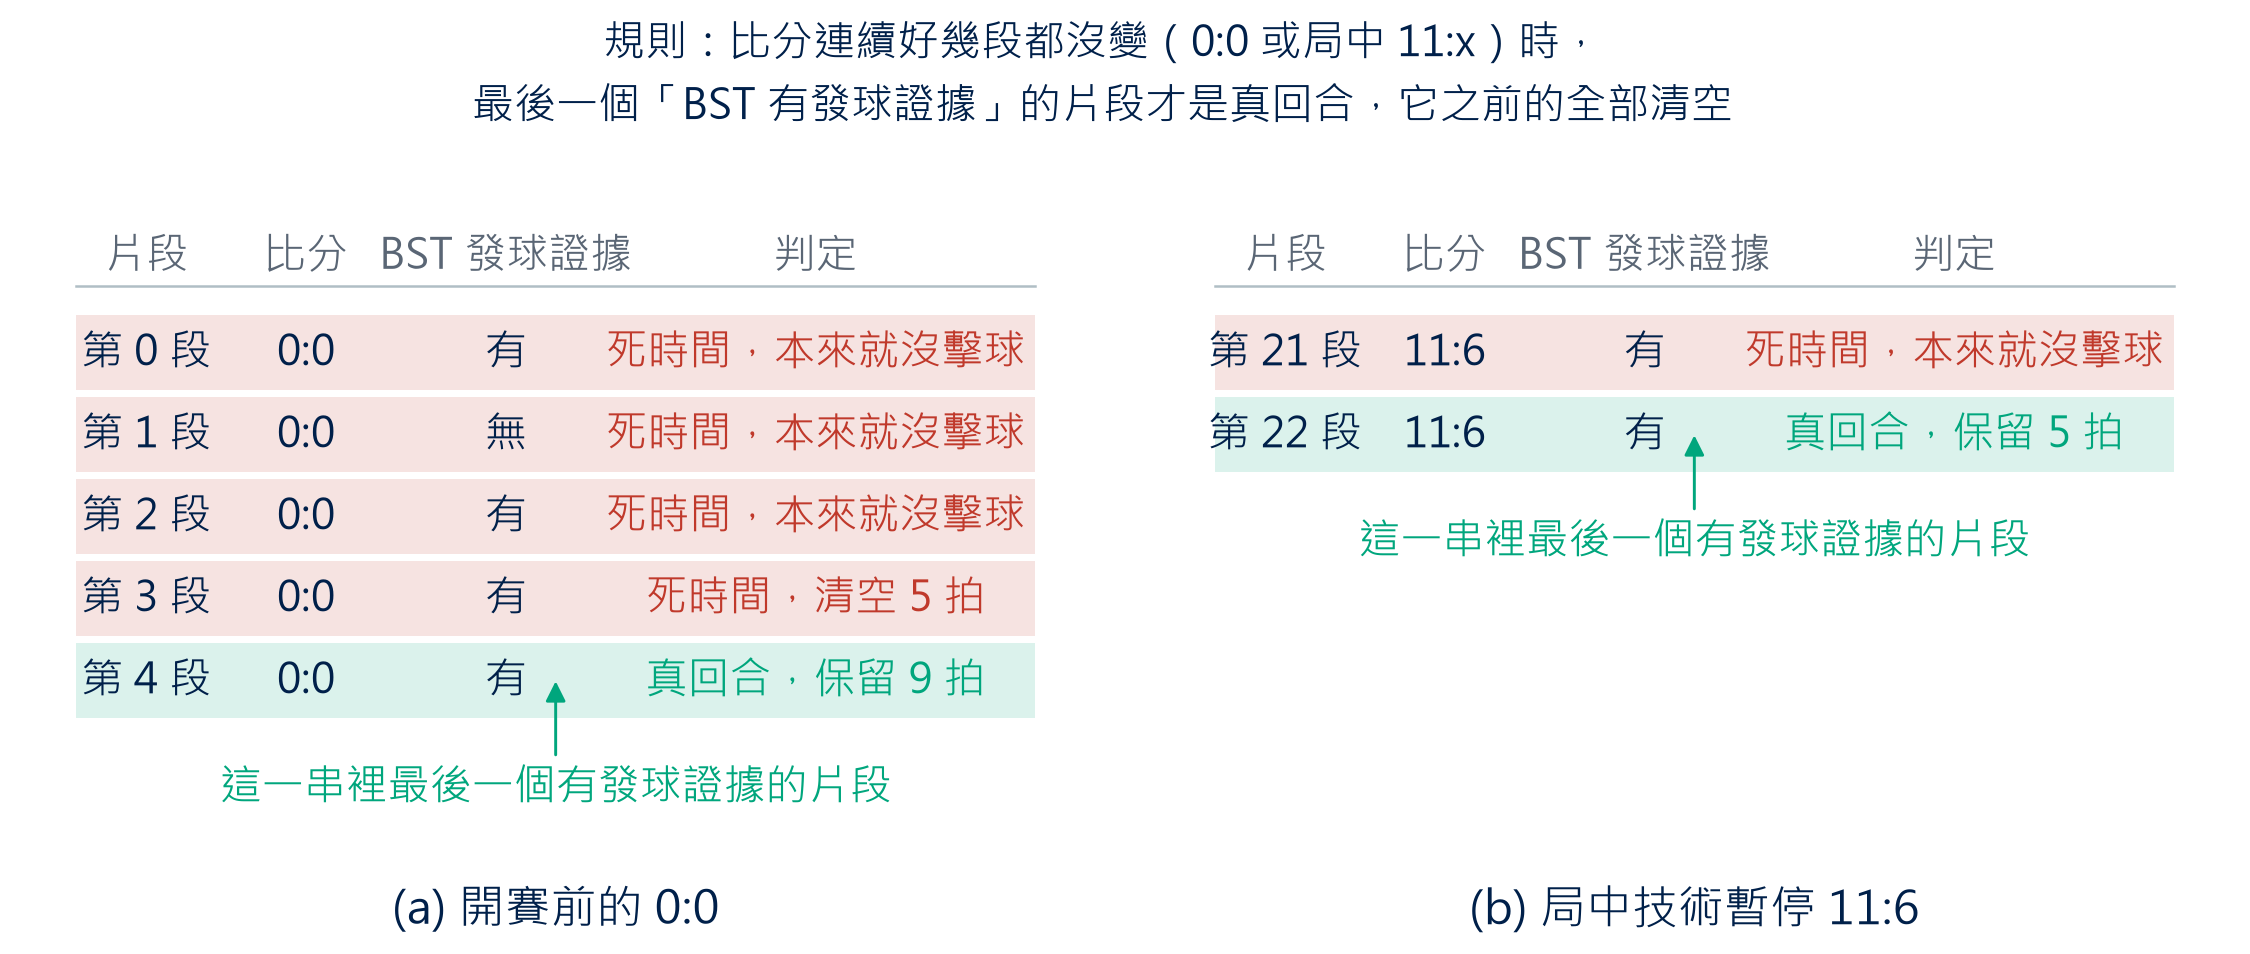
\includegraphics[width=\linewidth]{event_detection/prune_scoreboard.png}
  \caption{結合比分與發球證據判定計分板死時間}
  \label{fig:prune-scoreboard}
\end{figure}

\subsection{球種分類}
\label{sec:stroke-classification}

\subsubsection{概述}

\textbf{問題與目標：}本階段根據每一次擊球前後的球員姿態、場上位置與羽球軌跡，判斷擊球者及球種。

\textbf{設計重點：}球種分類器採用預訓練的 Badminton Stroke-type Transformer（BST）~\cite{bst}，本專題不重新訓練或修改其模型架構。BST 解決的是「已知擊球時刻及各項特徵後，如何判斷球種」。本專題在球種分類上的重點在於，利用前述各模組，自動從原始比賽影片產生 BST 所需的全部輸入。

\textbf{處理流程總覽：}如\figref{fig:stroke-classification-flow}。

\begin{figure}[H]
  \centering
  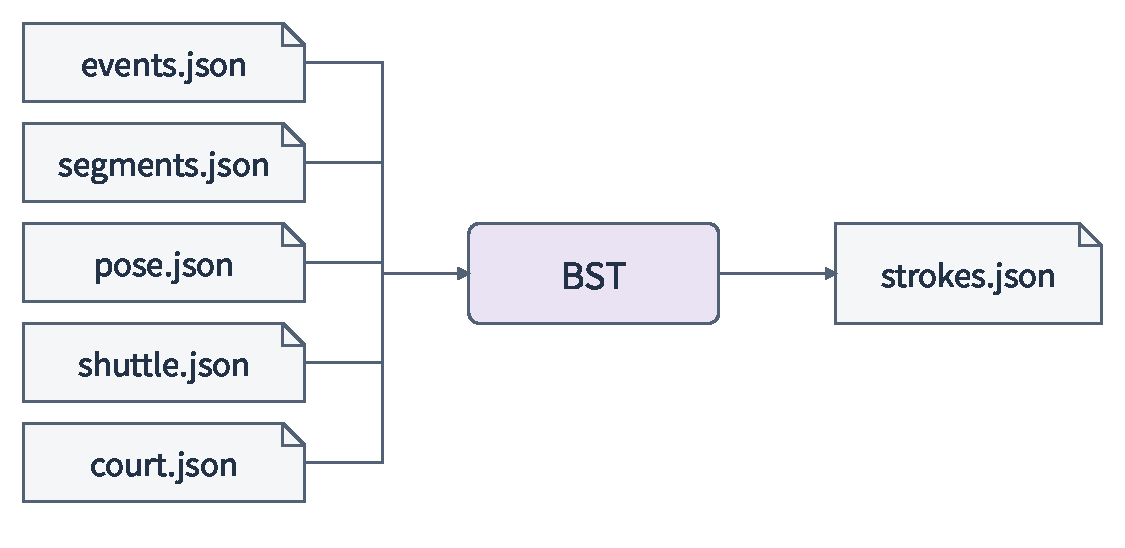
\includegraphics[scale=\flowscale]{stroke-classification.pdf}
  \caption{球種分類處理流程}
  \label{fig:stroke-classification-flow}
\end{figure}

\subsubsection{分類流程}

系統先將每個擊球時刻歸入對應回合，再依 BST 預訓練權重所使用的方式，以相鄰擊球時刻切出分析窗口。窗口內的球員骨架、場上位置與羽球軌跡會按照 BST 的資料格式進行正規化，並統一整理為 100 幀的輸入序列（\figref{fig:bst-window}）。

整理後的資料送入預訓練 BST，模型輸出 25 類機率（\figref{fig:bst-output}），將結果依賽評需求整理為 8 類：高遠球、發球、小球、平快球、殺球、切球、撲球與勾球。若模型輸出未知類別，系統保留為未知。

\begin{figure}[H]
  \centering
  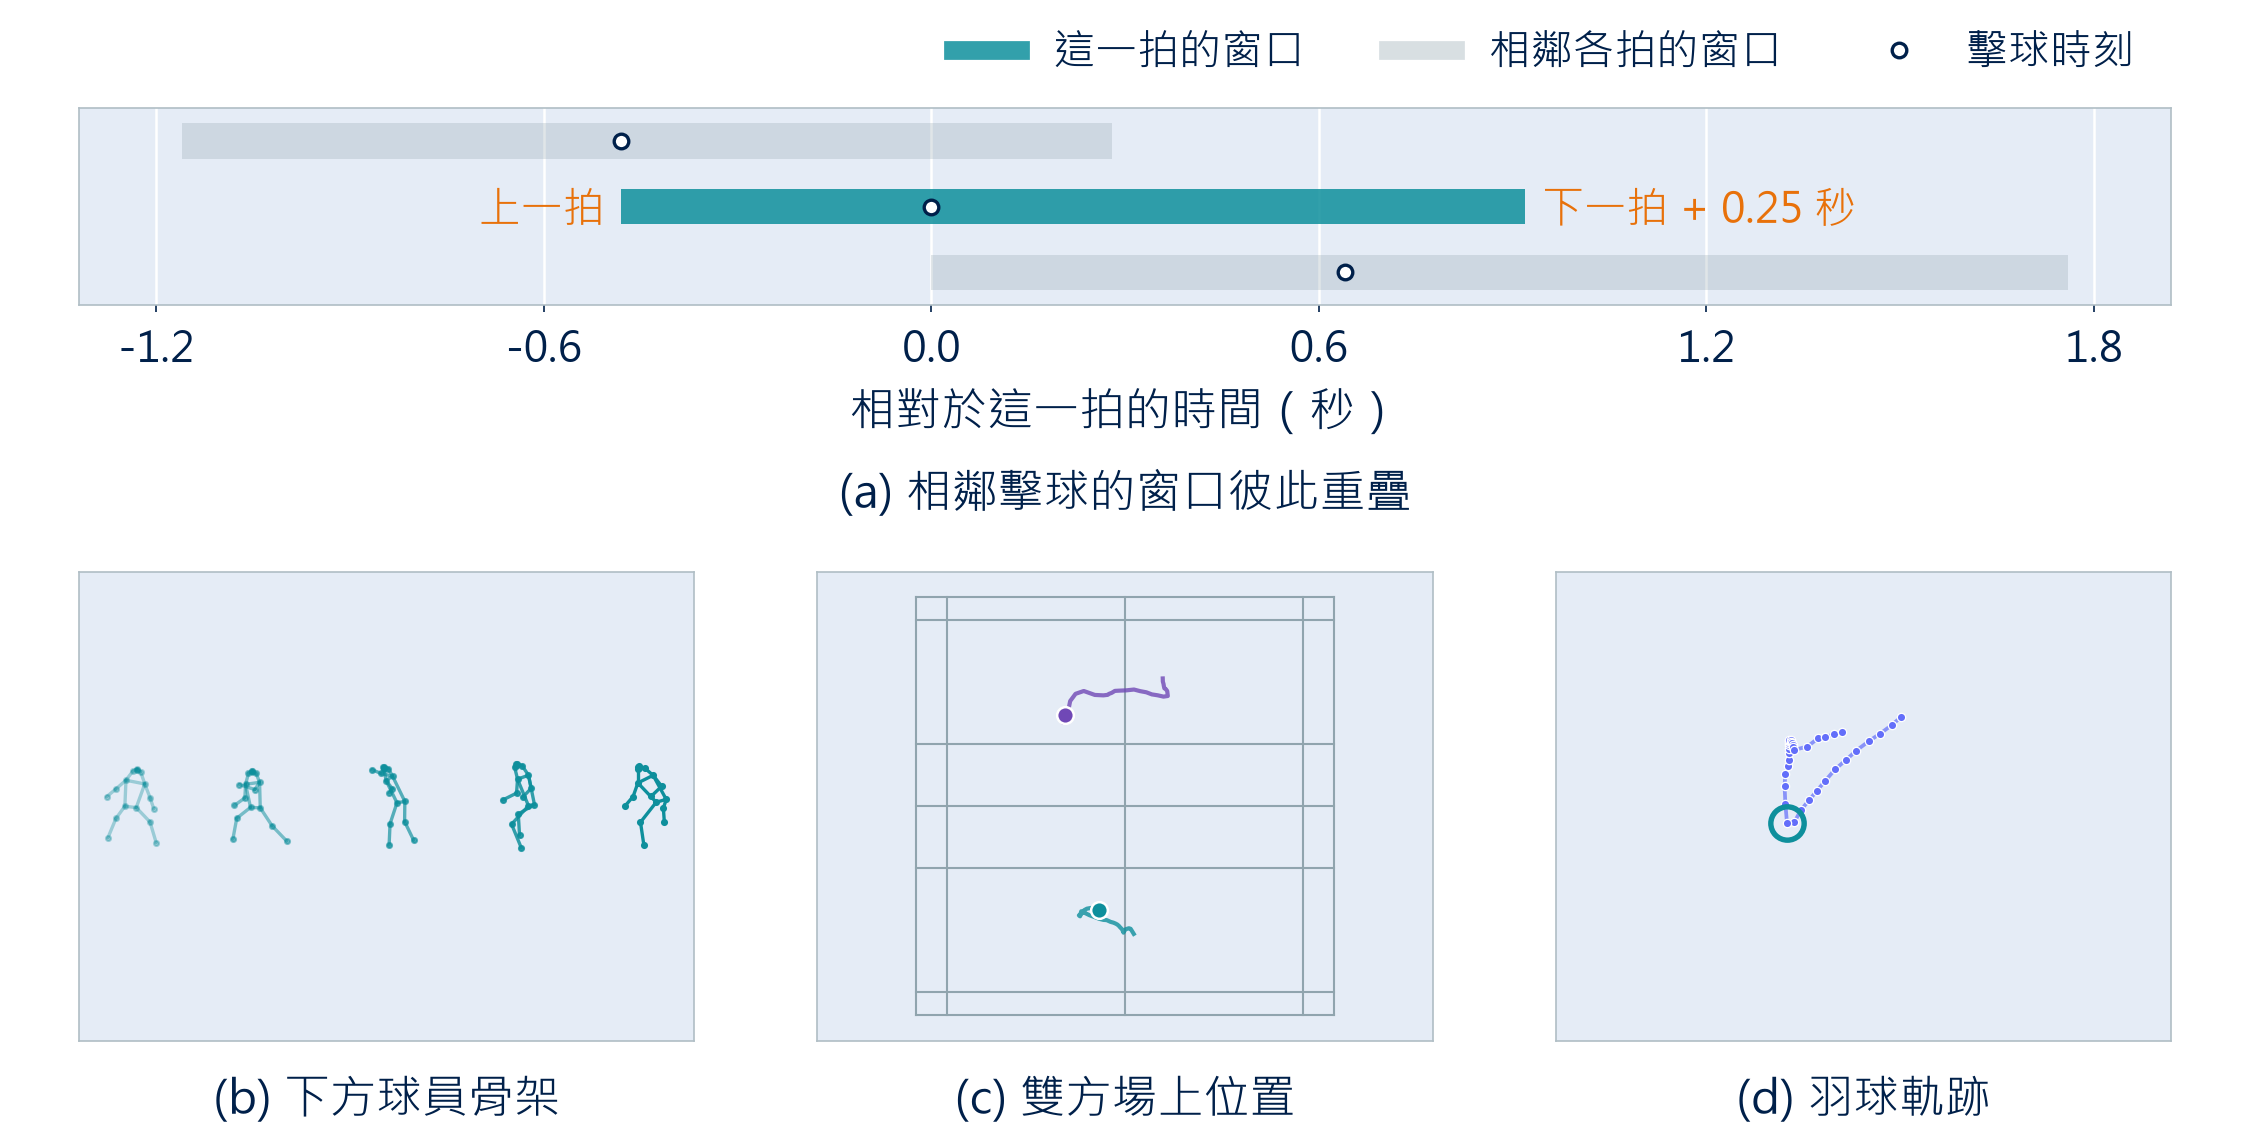
\includegraphics[width=\linewidth]{stroke_classification/bst_window.png}
  \caption{依相鄰擊球時刻建立 BST 的 100 幀輸入窗口}
  \label{fig:bst-window}
\end{figure}

\begin{figure}[H]
  \centering
  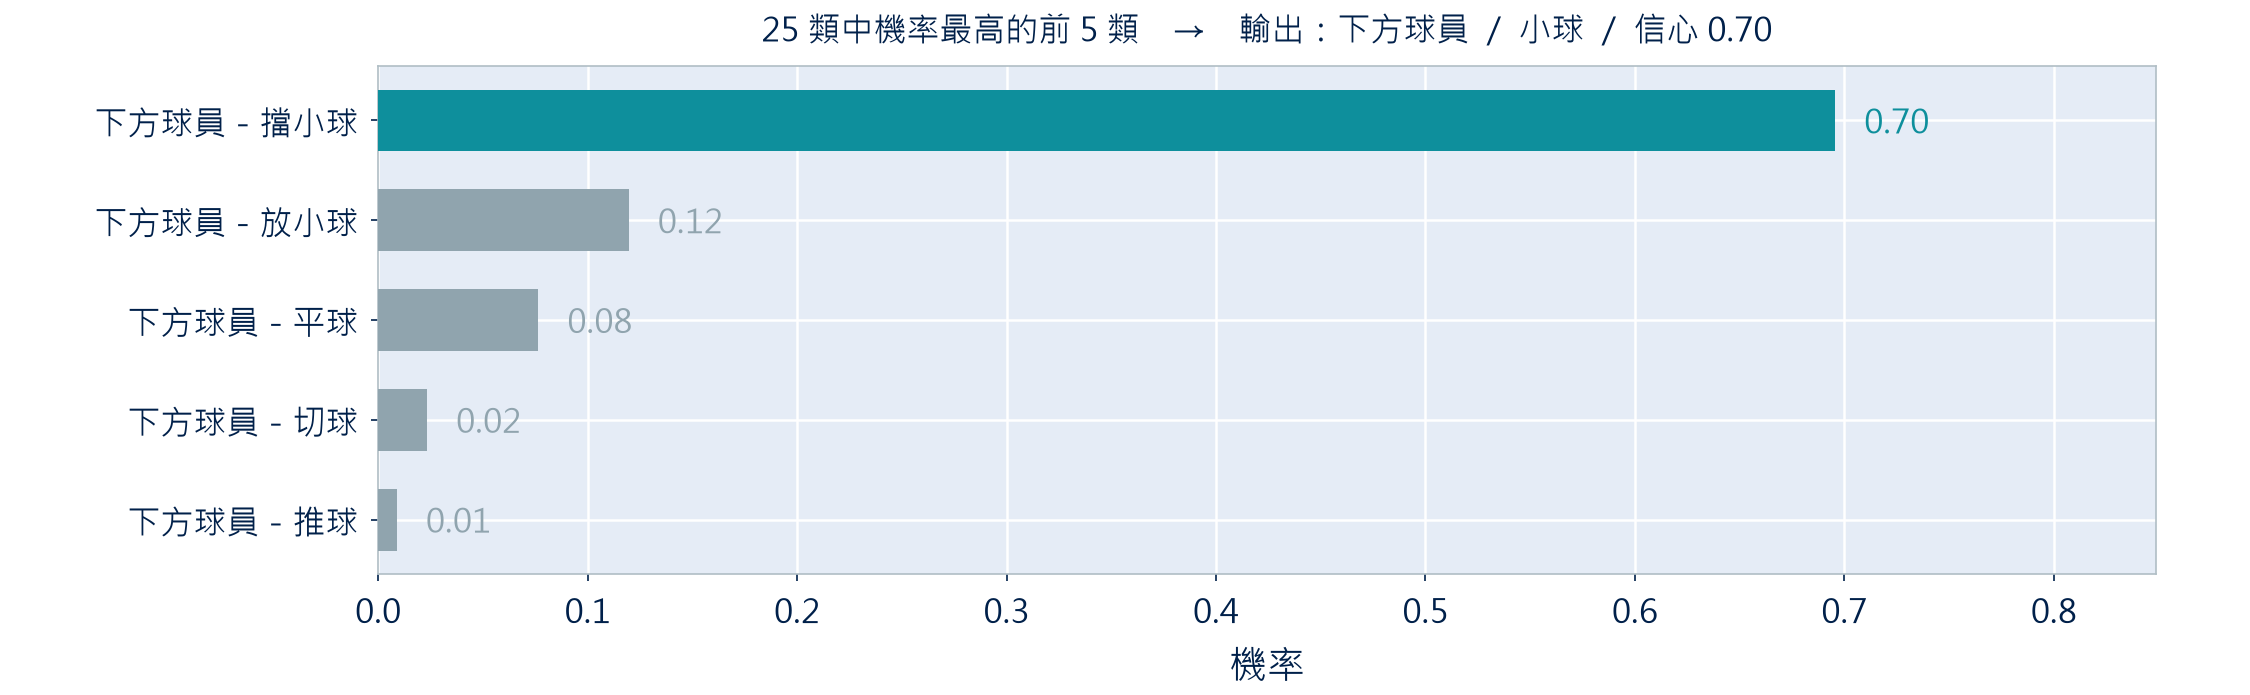
\includegraphics[width=\linewidth]{stroke_classification/bst_output.png}
  \caption{BST 的 25 類預測}
  \label{fig:bst-output}
\end{figure}

\section{音訊與精彩度分析}
\label{sec:audio-highlights}

\subsection{歡呼音訊量測}
\label{sec:cheer-audio}

\subsubsection{概述}

\textbf{問題與目標：}視覺模組能說明每一拍發生了什麼，卻無法判斷哪個回合最讓現場有反應。觀眾歡呼是轉播中現成的精彩度訊號。本模組以分段模組產生的每個片段為範圍，量測片段結束前後是否出現歡呼及其相對強度，作為精彩片段排序的依據。

\textbf{設計重點：}本模組不從頭訓練音訊模型，而是以凍結的 YAMNet~\cite{yamnet} 擷取通用音訊特徵，只在其上訓練一個輕量的邏輯迴歸分類器，因此 400 個人工標註窗口就足以完成訓練。歡呼多在回合結束的瞬間爆發，所以讀取範圍會延伸到片段結束後 3 秒。分類與強度分開估計：分類器判斷窗口裡有沒有歡呼，響度則衡量歡呼有多大聲，兩者再各自聚合為每個片段一筆量測。音訊只是視覺分析的補充，不建立或覆寫擊球、球種、比分與球員身分等競賽事實，缺少音訊時，其餘模組仍照常運作。以 4 場比賽逐場交叉驗證，窗口層級歡呼偵測的 macro F1 為 0.827、ROC-AUC 為 0.957（見\secref{sec:exp-cheer}）。

\textbf{處理流程總覽：}如\figref{fig:audio-cheer-flow}。

\begin{figure}[H]
  \centering
  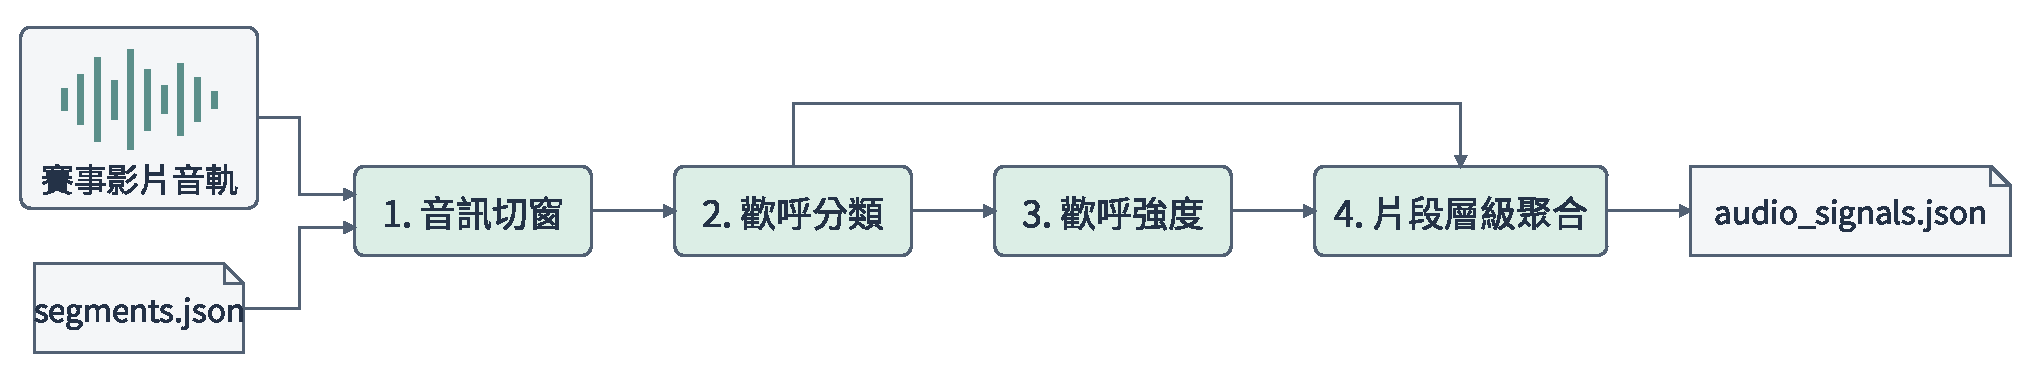
\includegraphics[scale=\flowscale]{audio-cheer.pdf}
  \caption{歡呼音訊量測處理流程}
  \label{fig:audio-cheer-flow}
\end{figure}

\subsubsection{音訊切窗}

系統先將音訊統一轉為 16 kHz 單聲道。對片段 $s$，分析起點等於片段起點，終點則延伸到片段結束後 3 秒，並以影片長度為上限：
\begin{equation}
  A_s^{start}=S_s^{start},\qquad
  A_s^{end}=\min(S_s^{end}+3,\;T_{media})
\end{equation}
延伸的原因是歡呼往往在回合結束時才開始，並在片段結束後持續數秒。分析範圍以 3 秒窗口切分，相鄰窗口的 hop 為 1 秒，只保留完整落在範圍內的窗口，尾端不足 3 秒的窗口直接捨棄（\figref{fig:audio-windows}）。相鄰片段各自切窗，因此兩者的窗口可能重疊。

\begin{figure}[H]
  \centering
  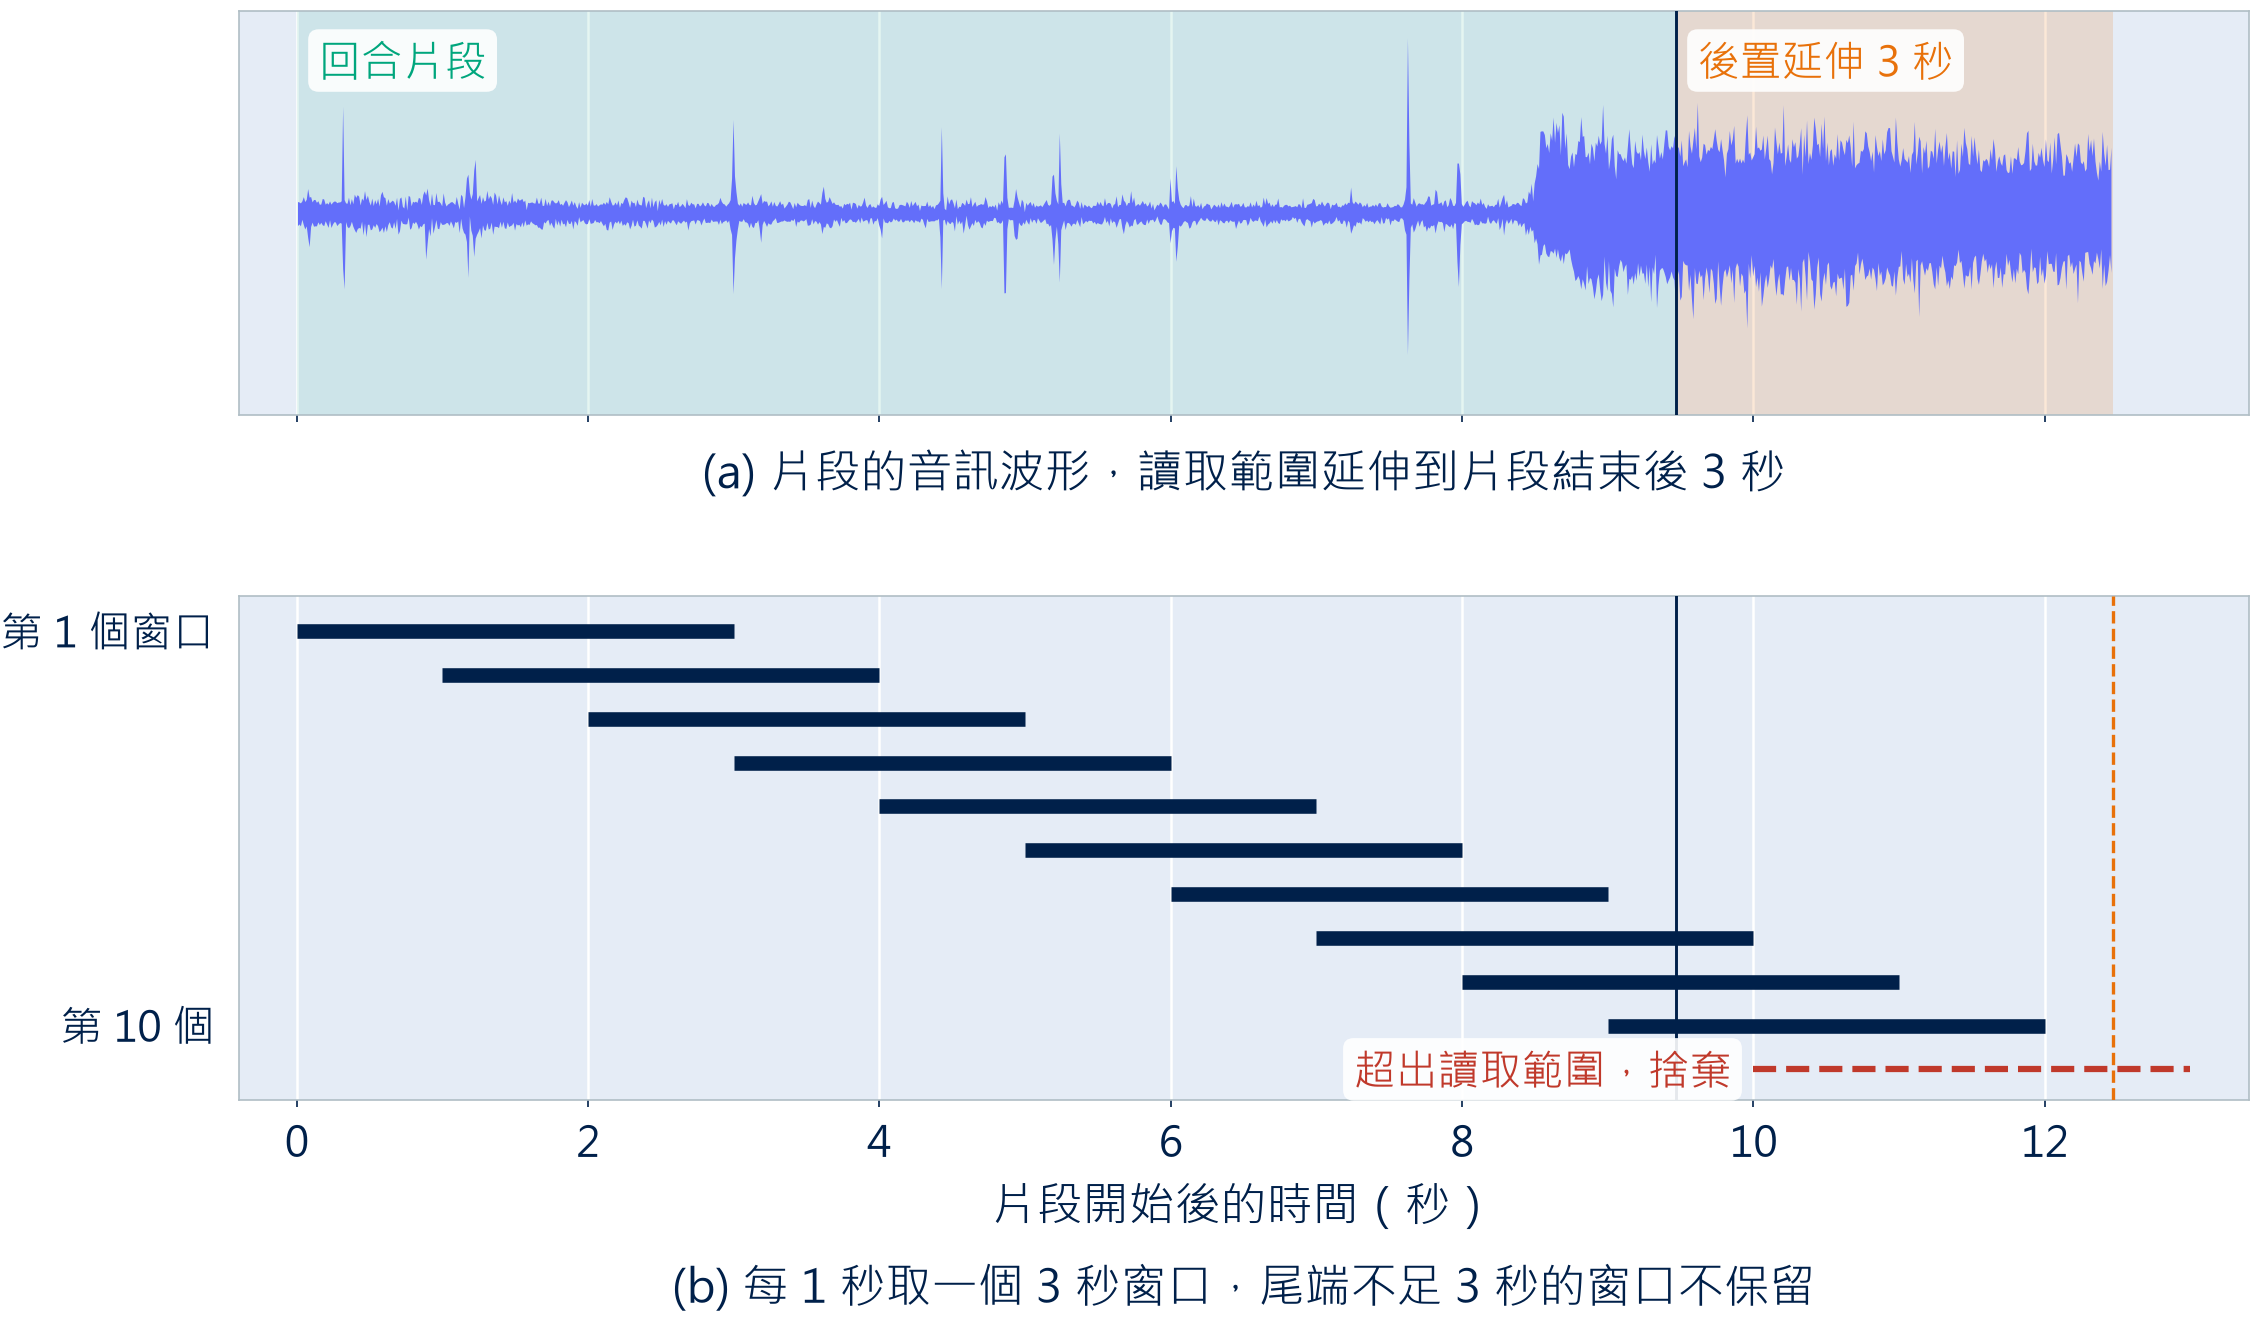
\includegraphics[width=\linewidth]{audio_highlight/audio_windows.png}
  \caption{片段音訊的讀取範圍與切窗}
  \label{fig:audio-windows}
\end{figure}

\subsubsection{歡呼分類}

每個 3 秒窗口輸入凍結的 YAMNet~\cite{yamnet}。YAMNet 以 AudioSet~\cite{audioset} 音訊事件資料預訓練，對一個窗口輸出多個時間切片的 1024 維特徵向量（patch embedding），系統取其平均作為窗口的固定長度表示：
\begin{equation}
  \mathbf{e}_i=\frac{1}{K_i}\sum_{k=1}^{K_i}\mathbf{z}_{i,k},
  \qquad \mathbf{e}_i\in\mathbb{R}^{1024}
\end{equation}
其中 $\mathbf{z}_{i,k}$ 為第 $i$ 個窗口的第 $k$ 個時間切片特徵，$K_i$ 為切片數。平均向量經標準化後送入邏輯迴歸，輸出窗口的歡呼分數 $p_i\in[0,1]$；$p_i\ge 0.5$ 的窗口視為正例窗口。

本系統不直接使用 YAMNet 原生的 Cheering 類別分數。在相同的逐場交叉驗證下，原生分數的 ROC-AUC 只有 0.839，以特徵向量訓練的分類器則為 0.957（見\secref{sec:exp-cheer}）。歡呼分數是分類器的輸出，未經機率校準，只用於門檻判斷與排序，不應解讀為歡呼發生的機率。

\subsubsection{歡呼強度估計}

同樣被判為歡呼，全場起立的喝采與零星掌聲在響度上可能差很多。因此系統另以窗口波形 $x_1,\ldots,x_N$ 的均方根（RMS）衡量響度：
\begin{equation}
  RMS_i=\sqrt{\frac{1}{N}\sum_{n=1}^{N}x_n^2},\qquad
  L_i=20\log_{10}(RMS_i+10^{-12})
\end{equation}
不同轉播的錄音音量差異很大，絕對響度無法跨比賽比較，因此系統只在單場比賽內比較。將全場 $M$ 個正例窗口的 $L_i$ 由小到大排名（從 0 起算，同值取平均排名），再除以 $M-1$ 映射到 $[0,1]$，得到窗口的歡呼強度 $r_i$。全場只有一個正例窗口時，強度定為 0.5。負例窗口不計算強度。$r_i$ 表示這個窗口在本場所有歡呼中的響度排名，而不是實際音壓。

\subsubsection{片段層級聚合}

每個片段約有十多個窗口，需要聚合為一筆量測。歡呼通常只占片段的最後幾秒，取平均會被前段大量的安靜窗口稀釋，取最大值則容易被單一誤判窗口左右。系統因此折衷採用線性內插的第 95 百分位數（p95）。令 $W_s$ 為片段 $s$ 的全部窗口、$W_s^+$ 為其中的正例窗口：
\begin{gather}
  C_s=Q_{0.95}^{linear}(\{p_i\mid i\in W_s\}),\qquad N_s=|W_s^+| \\
  I_s=
  \begin{cases}
    Q_{0.95}^{linear}(\{r_i\mid i\in W_s^+\}), & |W_s^+|>0\\
    \mathrm{null}, & |W_s^+|=0
  \end{cases}
\end{gather}
$C_s$ 為片段歡呼分數，聚合片段內全部窗口；$I_s$ 為片段歡呼強度，只聚合正例窗口，沒有正例時為空值；$N_s$ 為正例窗口數。由於窗口彼此重疊，$N_s$ 不等於獨立的歡呼次數。各聚合方法的比較見\secref{sec:exp-aggregation}。

\subsection{精彩片段排序}
\label{sec:highlight-ranking}

\subsubsection{概述}

\textbf{問題與目標：}本模組把每個片段的歡呼量測合成一個精彩度分數，將整場比賽的片段由精彩到平淡排序，供回看介面標示重要回合，也作為賽評生成的選用背景訊號。

\textbf{設計重點：}目前沒有人工標註的精彩片段真值可供訓練，因此精彩度分數採用透明的固定公式，而不是學習得到的模型。沒有歡呼的片段，強度以 0 計：
\begin{equation}
  H_s=0.5\,C_s+0.5\,I_s^{effective},\qquad
  I_s^{effective}=
  \begin{cases}
    I_s, & I_s\neq\mathrm{null}\\
    0, & I_s=\mathrm{null}
  \end{cases}
\end{equation}
分數相同時，依片段歡呼分數、再依片段先後排序。0.5／0.5 的權重只表示等量結合「有沒有歡呼」與「歡呼多大聲」，並非最佳化的結果。由於強度是單場內的相對量，精彩度分數也只能在同一場比賽內比較。

\textbf{處理流程總覽：}如\figref{fig:highlight-ranking-flow}。

\begin{figure}[H]
  \centering
  
\includegraphics[scale=\flowscale]{highlight-ranking.pdf}
  \caption{精彩片段排序處理流程}
  \label{fig:highlight-ranking-flow}
\end{figure}

\section{賽事理解}
\label{sec:match-understanding}

\subsection{球員身分對應}
\label{sec:player-identity}

\subsubsection{概述}

\textbf{問題與目標：}球種分類只知道擊球者位在畫面上方或下方，賽評卻需要指名選手。本階段判斷在每兩次換邊之間，上下方球員各是計分板上的哪一位選手。

\textbf{設計重點：}本階段不需要人工標註，主要也不依賴球員外觀，而是由既有的兩項結果推得。比分變化指出計分板上的哪一位選手發球，回合第一拍的擊球者指出發球者在上方或下方，兩者結合即為一次對應。換邊的時間點由羽球規則決定（第一局結束、第二局結束、決勝局領先方達 11 分），只需從比分推算，不必從畫面偵測。

\textbf{處理流程總覽：}如\figref{fig:identity-mapping-flow}。

\begin{figure}[H]
  \centering
  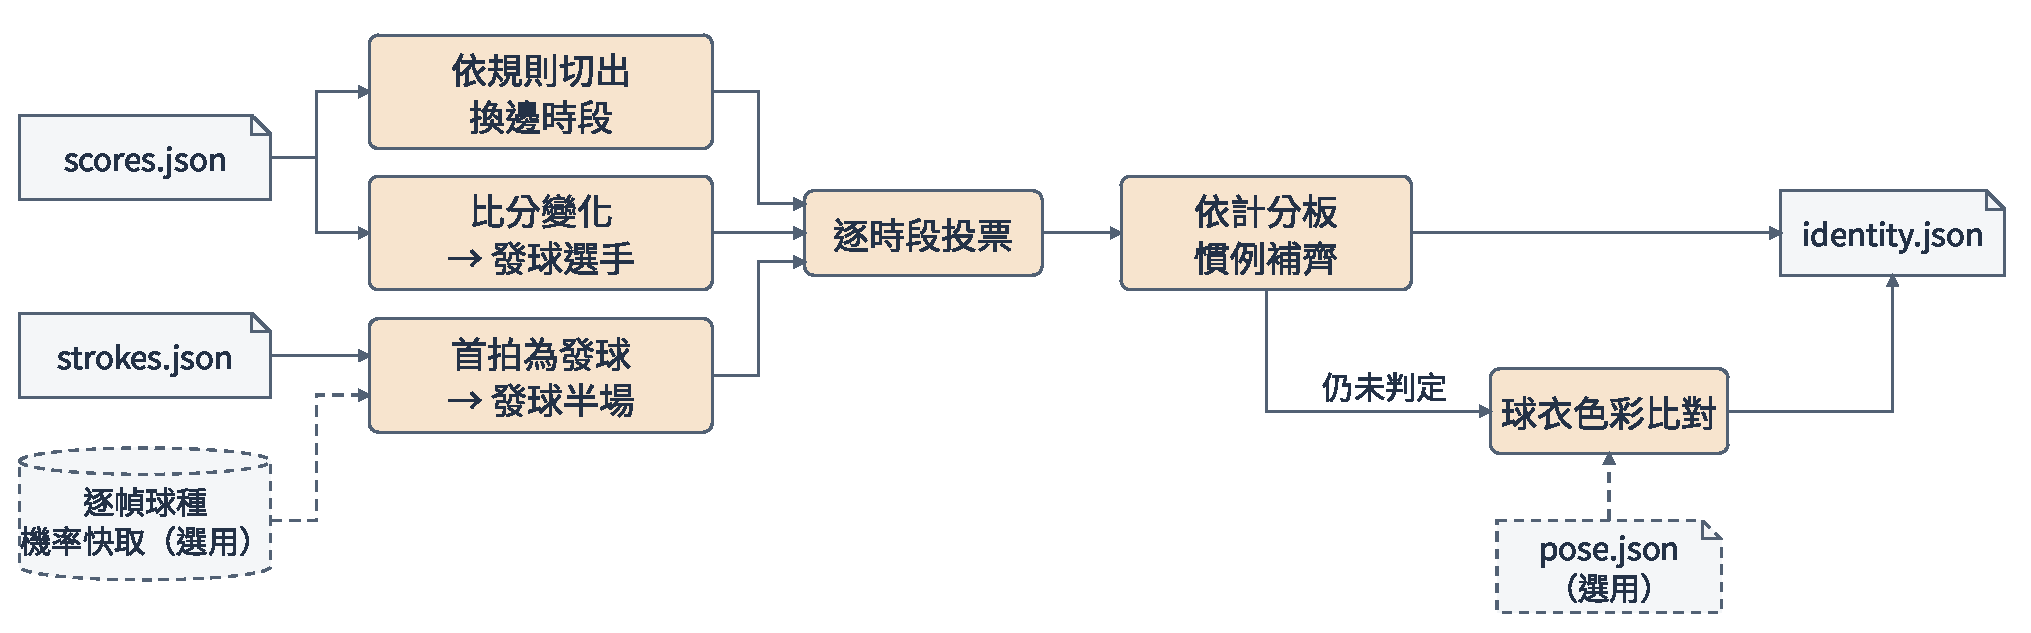
\includegraphics[scale=\flowscale]{identity-mapping.pdf}
  \caption{球員身分對應處理流程}
  \label{fig:identity-mapping-flow}
\end{figure}

\subsubsection{判定流程}

\textbf{誰發球。}落地得分制下，贏得回合的一方發下一球。\texttt{scores.json} 記錄的是回合開始前的比分，所以比較相鄰兩個片段，比分剛好加一分的選手就是下一個片段的發球者。

\textbf{發球者在哪一側。}回合第一拍的擊球者所在的半場，就是發球者的半場。但若擊球時刻偵測漏掉發球，第一拍其實是接發球，半場會整個判反。因此只採用 BST 判為發球的第一拍。其餘回合再從擊球時刻偵測的逐幀球種機率中找回發球，且只在發球類別與擊球者都明顯佔優時採用。

\textbf{投票與補齊。}同時知道發球選手與發球半場的回合各投一票，同一換邊時段內取多數。票數不足 5 票的時段，沿用最近已判定時段的結果，並依計分板慣例調整：列序固定的計分板每次換邊對調一次，隨場地換列的則不變。採用哪種慣例，由已判定時段之間是否對調推得。仍無法判定時，才比對兩側球員上衣與褲子的 HSV 色彩；連外觀也分不出來就留空，不做猜測。每個時段的判定依據（投票、慣例或外觀）都寫入 \texttt{identity.json}。

\section{使用者介面}
\label{sec:user-interface}

\subsection{概述}

\textbf{問題與目標：}前述各模組的輸出是十多份 JSON 檔，記錄每個回合的起訖、比分、球員骨架、羽球軌跡等。這些資料必須對照影片才看得懂，直接閱讀數字既無法判斷分析是否正確。本系統的使用者介面讓使用者不必操作指令列，就能完成「匯入影片、執行分析、對照影片回看結果」的完整流程，並把逐拍資訊疊回轉播畫面，讓分析結果可以被直接檢視。

\textbf{使用流程總覽：}如\figref{fig:ui-workflow}。

\begin{figure}[H]
  \centering
  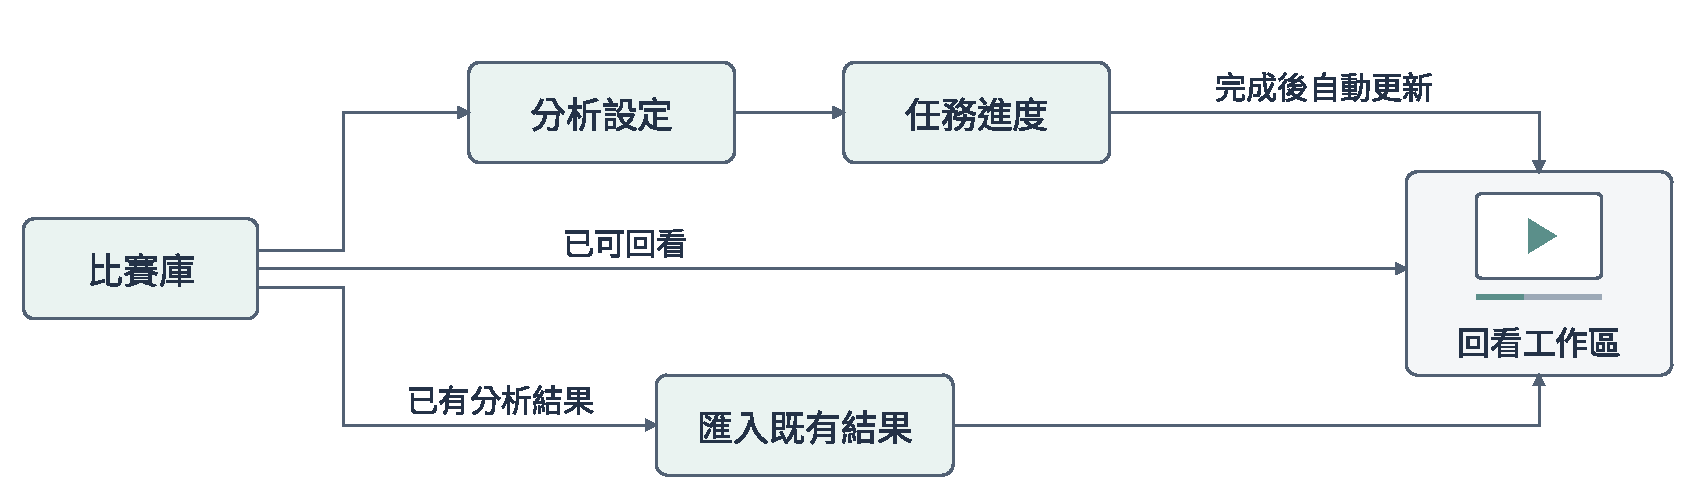
\includegraphics[scale=\flowscale]{ui-workflow.pdf}
  \caption{使用者介面操作流程}
  \label{fig:ui-workflow}
\end{figure}

比賽庫列出比賽資料夾中的每一場比賽及其分析狀態（\figref{fig:match-library}）。尚未分析的比賽從「分析設定」選擇要執行的項目（\figref{fig:analysis-settings}），分析在背景執行，完成後回看資料自動更新。已在其他環境完成分析的比賽，則可直接匯入既有結果，不需重新計算。

\begin{figure}[H]
  \centering
  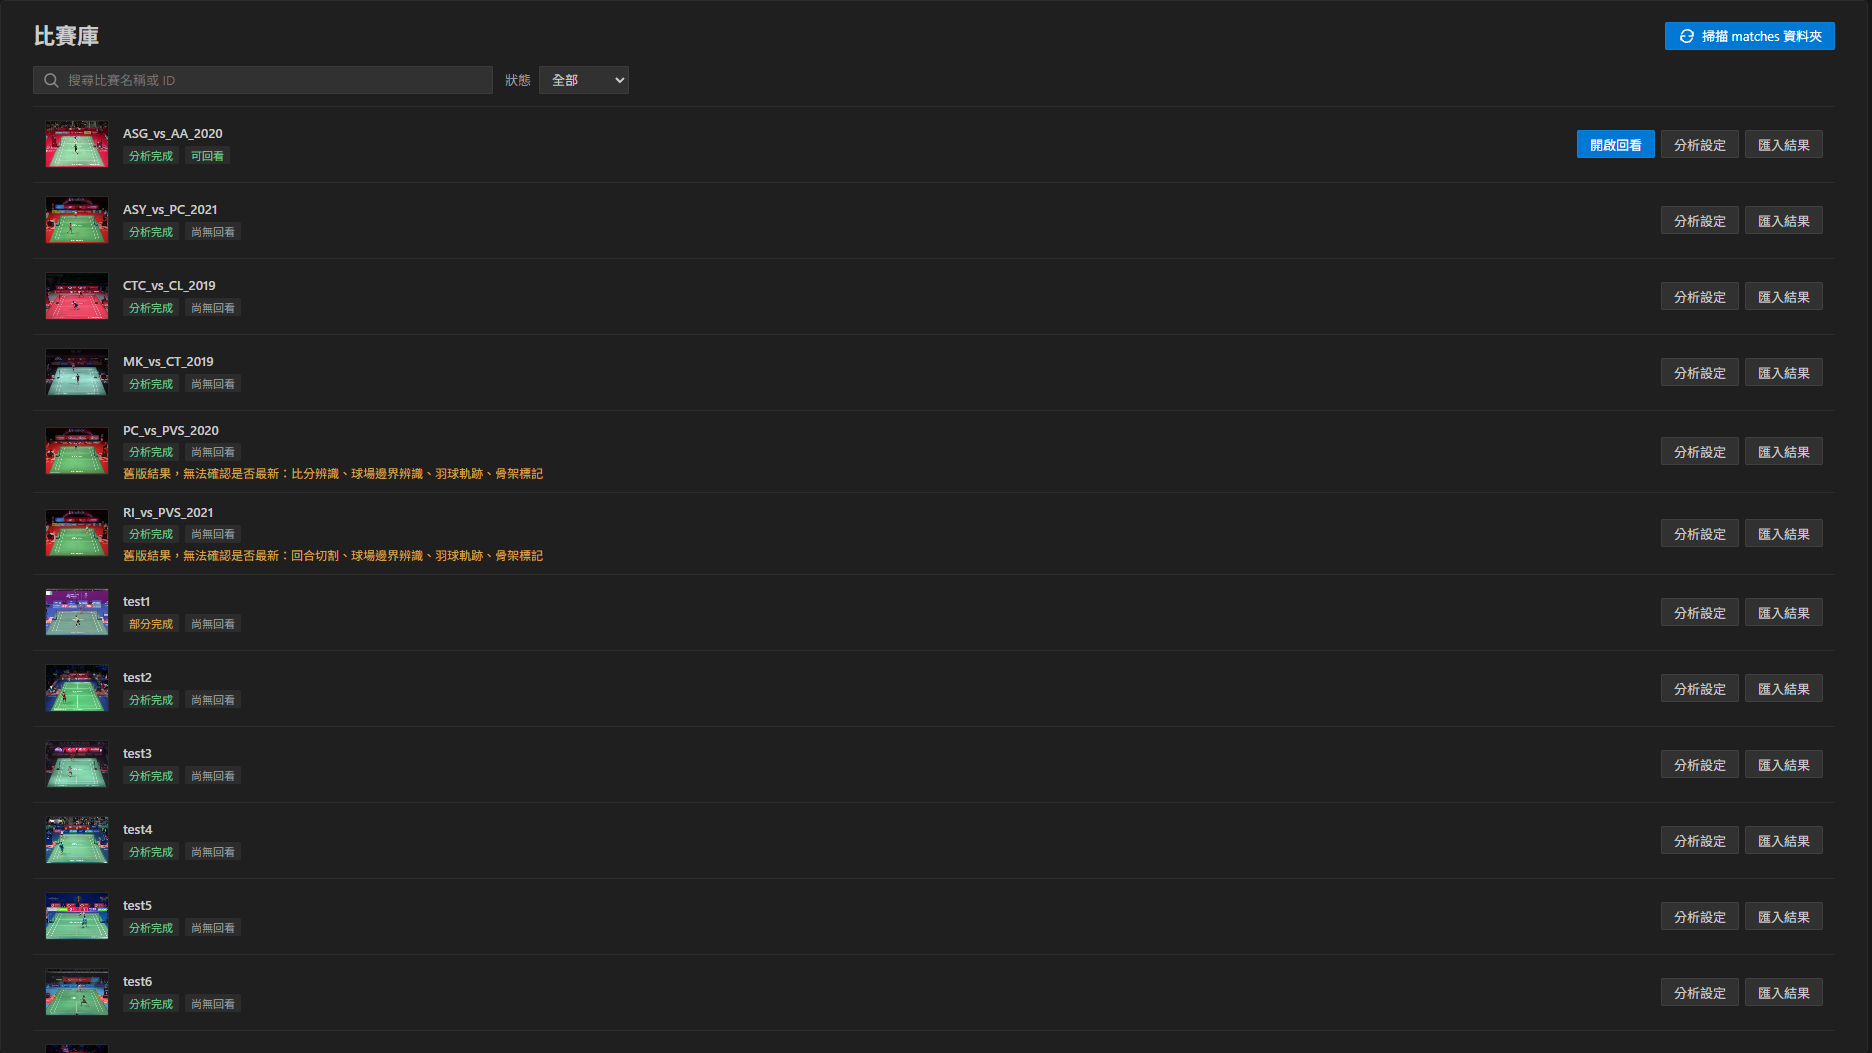
\includegraphics[width=\linewidth]{ui/match_library.png}
  \caption{比賽庫，每場比賽標示分析狀態與是否可回看}
  \label{fig:match-library}
\end{figure}

\begin{figure}[H]
  \centering
  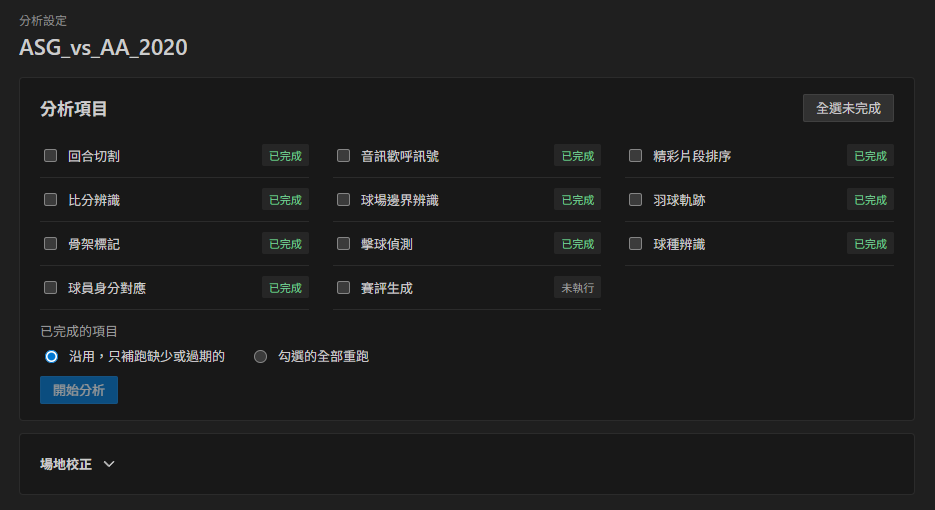
\includegraphics[width=0.850\linewidth]{ui/analysis_settings.png}
  \caption{分析設定，每個分析項目標示已完成、未執行或已過期}
  \label{fig:analysis-settings}
\end{figure}

\subsection{回看工作區}

回看工作區是介面的核心，由播放器、回合分析欄與時間軸三個區域組成（\figref{fig:review-workspace-full}）。三者共用同一個影片時間，任一區域的操作都會同步反映到另外兩區。

\begin{figure}[H]
  \centering
  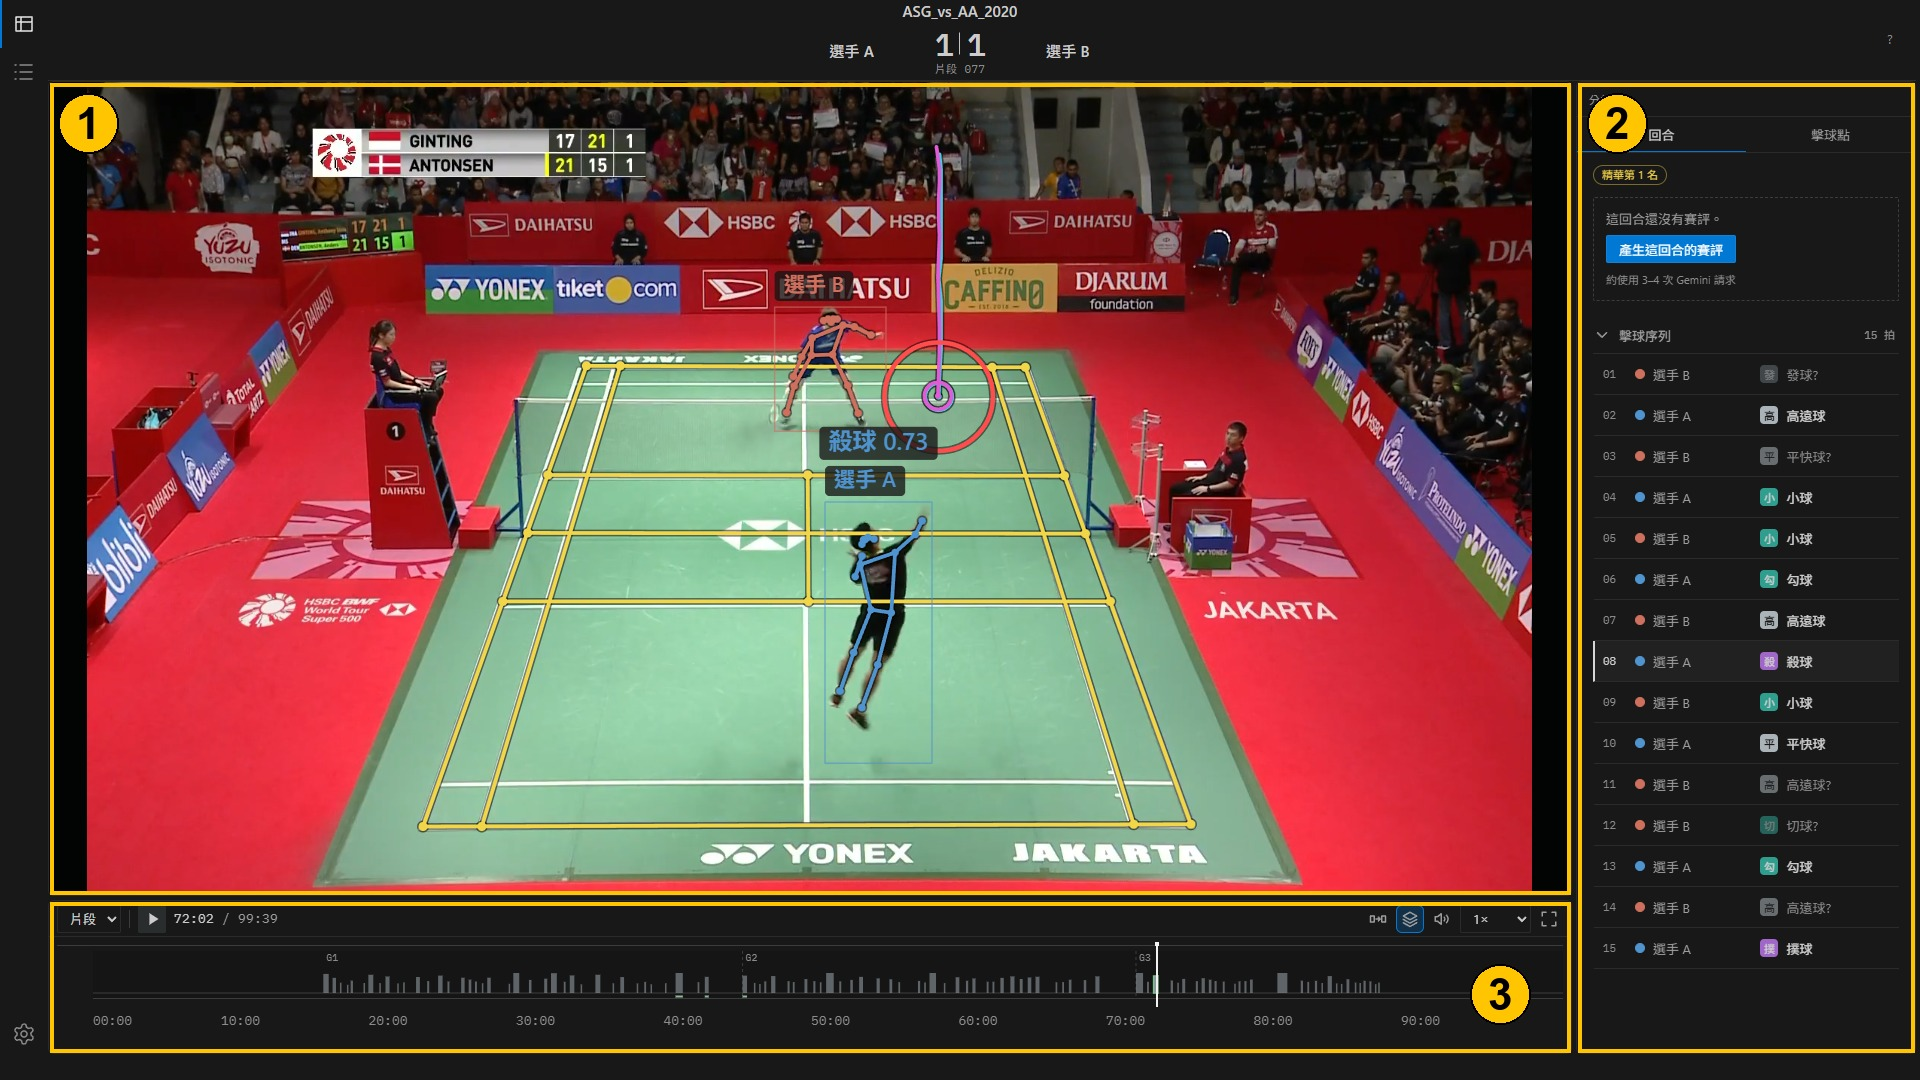
\includegraphics[width=\linewidth]{ui/review_workspace.jpg}
  \caption{回看工作區。\circnum{①} 播放器與疊圖 \circnum{②} 回合分析欄 \circnum{③} 時間軸}
  \label{fig:review-workspace-full}
\end{figure}

\subsubsection{播放器與疊圖}

播放器在轉播畫面上疊加各模組的分析結果，共 7 個圖層：球場線、骨架、選手標籤、羽球、球路拖尾、擊球閃圈與球種標籤（\figref{fig:overlay-layers}）。各圖層可以單獨開關，讓使用者直接用眼睛檢查各模組的結果，例如球場線是否貼合場地、骨架是否選對球員、軌跡是否跟著球走。

完整轉播中，回合只佔播出時間的約三成。「只播片段」模式會自動跳過回合之間的重播、休息與觀眾畫面，只播放分段模組切出的比賽片段。

\begin{figure}[H]
  \centering
  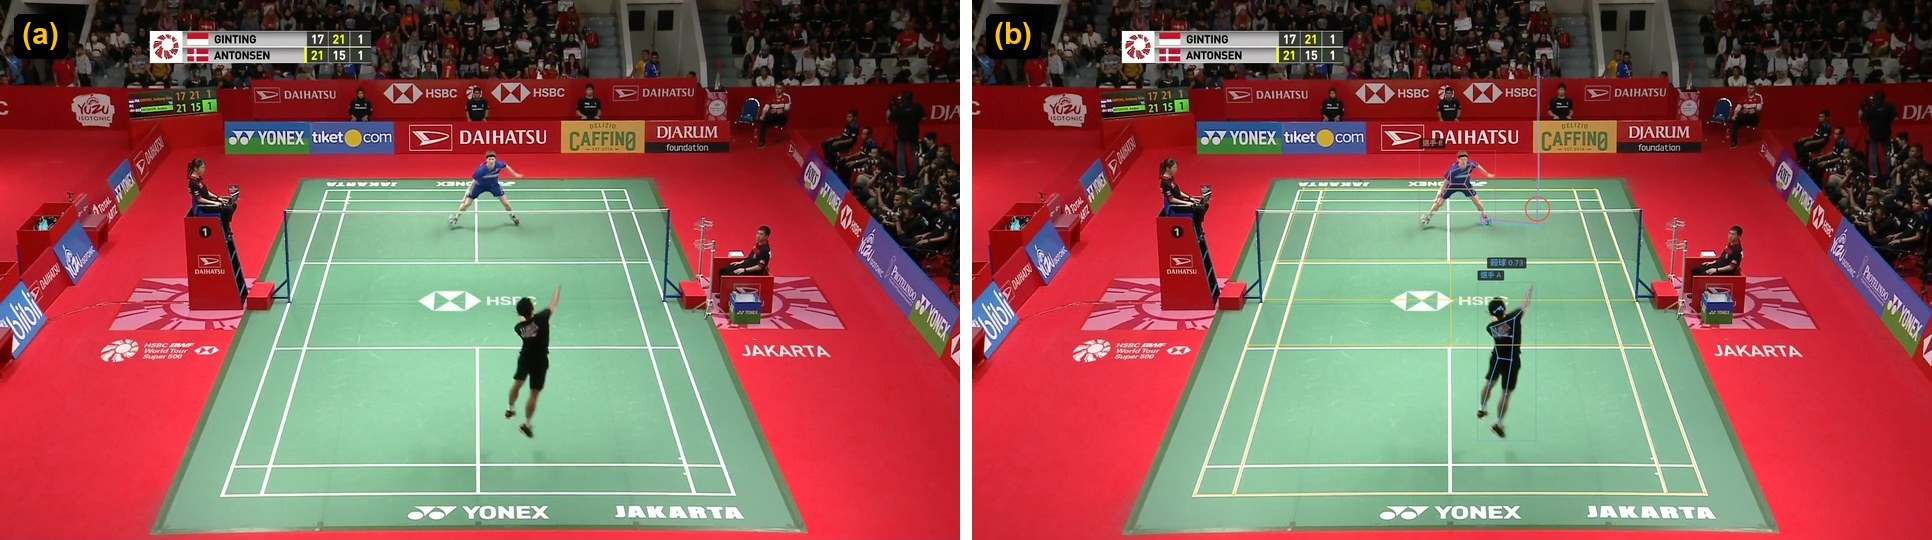
\includegraphics[width=\linewidth]{ui/overlay_layers.jpg}
  \caption{疊圖開啟前後。(a) 原始轉播畫面 (b) 開啟全部圖層}
  \label{fig:overlay-layers}
\end{figure}

\subsubsection{回合分析欄}

分析欄顯示目前回合的逐拍資訊，分為「回合」與「擊球點」兩個分頁（\figref{fig:inspector}）。

\begin{itemize}
  \item \textbf{擊球序列：}依序列出每一拍的擊球者與球種，信心度低於 0.5 的球種以淡色加問號標示。點選任一拍，影片即跳到該拍的擊球時刻。
  \item \textbf{精華標記：}精彩度排名在全場前 10\% 的回合，會在欄位頂端顯示排名徽章。
  \item \textbf{單回合賽評：}分析流程中的賽評階段只示範生成精彩排名前 3 的回合。其他回合由使用者在想看時按下「產生這回合的賽評」，每次約使用 3--4 次 Gemini 請求。產生後，回合摘要下方以「依據 \#1、\#2…」列出摘要所引用的擊球，點選即跳到該拍。逐拍賽評則附在擊球序列的每一拍下方，讓使用者能逐句對照影片確認賽評是否有所本。
  \item \textbf{擊球點：}以俯視球場標出本回合每一拍的擊球位置，依擊球順序連線，顏色區分兩名球員，可一眼看出回合中雙方的跑動與落點分布。
\end{itemize}

\begin{figure}[H]
  \centering
  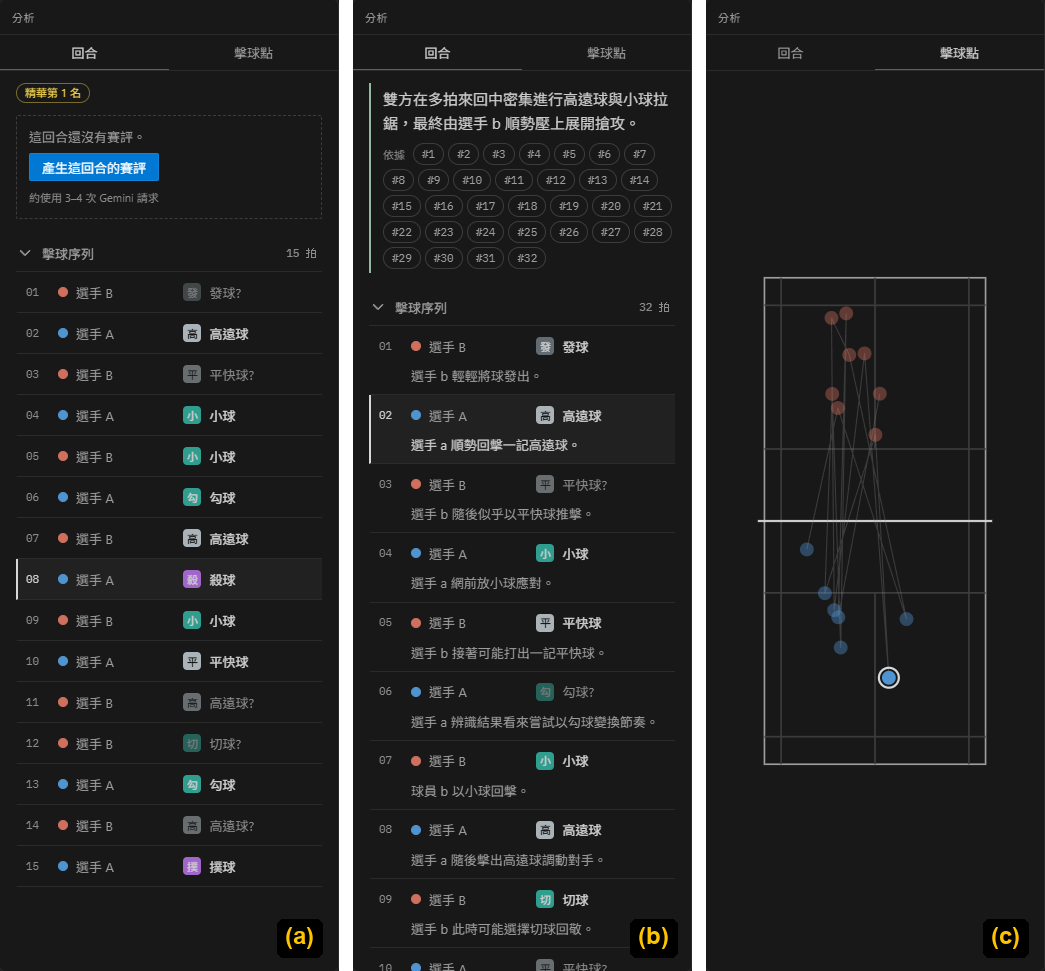
\includegraphics[width=0.950\linewidth]{ui/inspector.png}
  \caption{回合分析欄。(a) 擊球序列與精華排名 (b) 產生賽評後 (c) 擊球點分頁}
  \label{fig:inspector}
\end{figure}

\subsubsection{時間軸}

時間軸提供四種模式，各自呈現一種隨時間變化的分析結果（\figref{fig:timeline-modes}）。

\begin{itemize}
  \item \textbf{片段：}每個片段一根長條，高度為回合長度，並以 G1--G3 標示局數。
  \item \textbf{擊球：}依每片段的球種組成著色。
  \item \textbf{比分：}呈現雙方比分差距隨時間的變化，位於中線上方表示選手 A 領先、下方表示選手 B 領先。
  \item \textbf{歡呼：}顯示各片段的歡呼訊號，並以三角形與數字標示精彩度排名。
\end{itemize}

\begin{figure}[H]
  \centering
  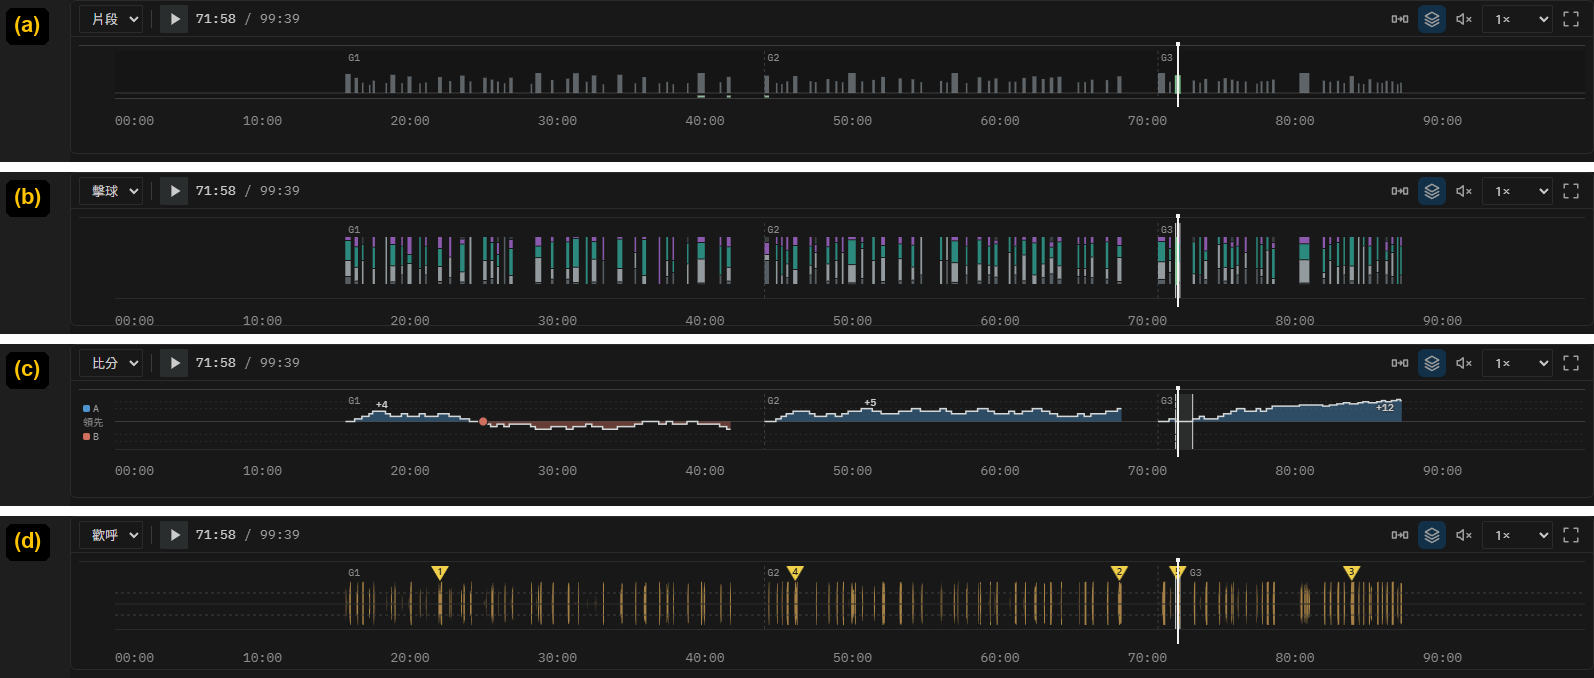
\includegraphics[width=\linewidth]{ui/timeline_modes.png}
  \caption{時間軸的四種模式（全場尺度）。(a) 片段 (b) 擊球 (c) 比分 (d) 歡呼}
  \label{fig:timeline-modes}
\end{figure}

時間軸可在「全場」與「單片段」兩種尺度間切換（\figref{fig:timeline-zoom}）。全場尺度用於掌握整場比賽的分布與走勢。雙擊任一片段即放大到該回合，此時每一拍成為一個點並標上球種縮寫，可以看出來回的節奏。

\begin{figure}[H]
  \centering
  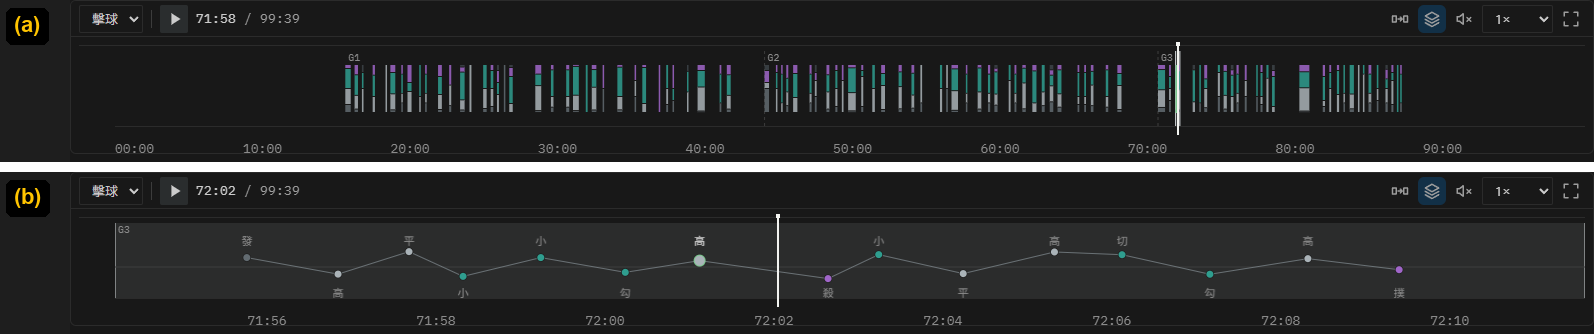
\includegraphics[width=\linewidth]{ui/timeline_zoom.png}
  \caption{擊球模式在兩種尺度下的呈現。(a) 全場 (b) 單回合}
  \label{fig:timeline-zoom}
\end{figure}

\subsection{分析任務與場地校正}

\textbf{分析計畫預覽：}使用者勾選分析項目時，介面即時列出執行計畫：哪些階段會執行、哪些沿用既有結果及其原因，以及計畫是否會呼叫 Gemini API（\figref{fig:plan-preview}）。若某些未勾選階段的上游結果會因這次分析而改變，介面也會列出這些將會過期的階段，回看時不會顯示過期的資料。

\begin{figure}[H]
  \centering
  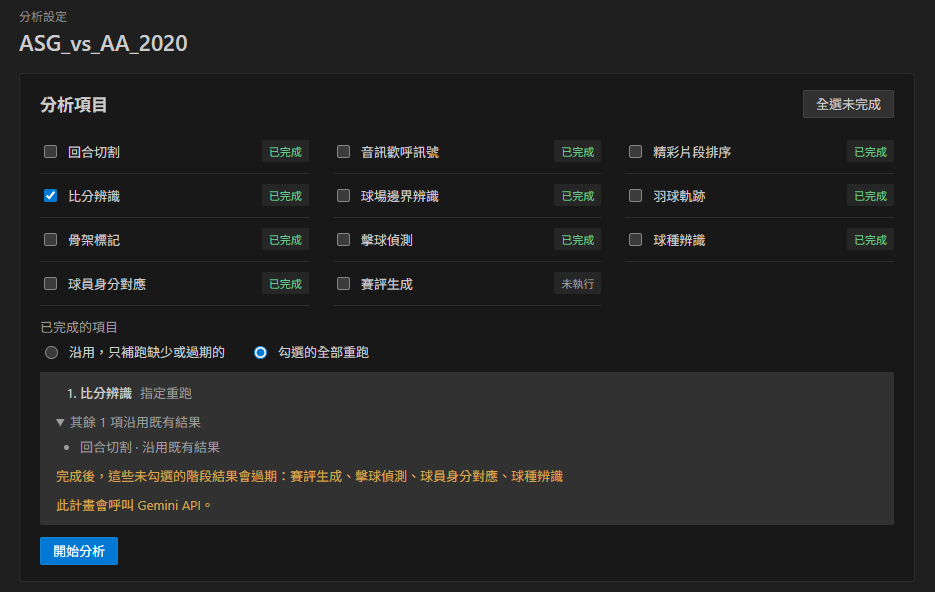
\includegraphics[width=0.850\linewidth]{ui/plan_preview.png}
  \caption{分析計畫預覽}
  \label{fig:plan-preview}
\end{figure}

\textbf{任務進度：}分析在獨立的背景程序中執行。任務頁顯示整體進度、各階段耗時與詳細記錄，使用者也可以隨時取消，取消時已完成的階段會保留，下次分析只需從中斷處繼續（\figref{fig:task-progress}）。

\begin{figure}[H]
  \centering
  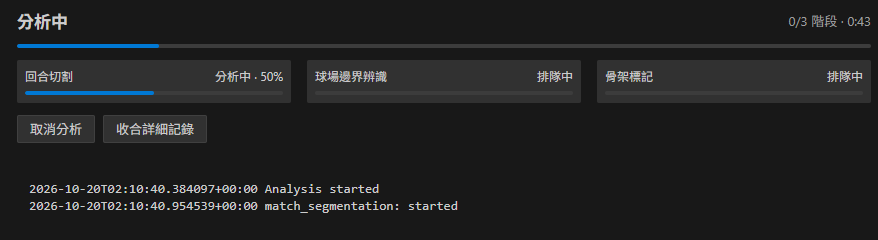
\includegraphics[width=0.798\linewidth]{ui/task_progress.png}
  \caption{任務進度，顯示整體與各階段的進度及詳細記錄}
  \label{fig:task-progress}
\end{figure}

\textbf{場地校正：}場地偵測是後續選人與站位換算的基礎，因此任務會先執行場地偵測，並把需要讀取球場的階段排到最後。球場一偵測完，介面即提示使用者檢查，分析設定頁自動展開場地預覽，其餘階段照常進行。若角點明顯偏移，使用者可直接在球場畫面上拖曳四個外角點，並以方向鍵逐像素微調（\figref{fig:court-calibration}）。保存後，尚未開始的階段直接使用新球場，已讀過舊球場的階段則自動重跑。

\begin{figure}[H]
  \centering
  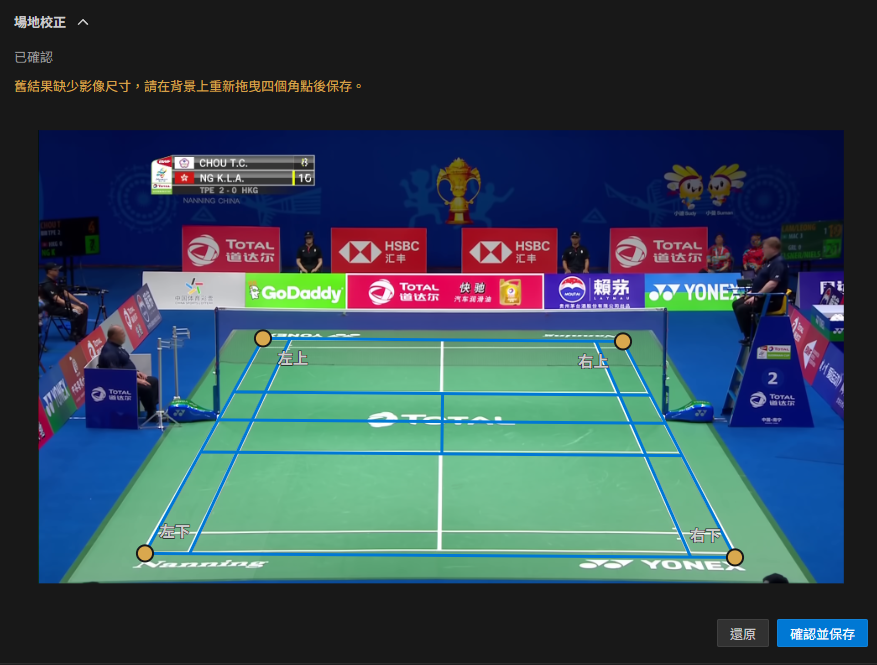
\includegraphics[width=0.797\linewidth]{ui/court_calibration.png}
  \caption{場地校正，拖曳四個外角點對齊球場邊線}
  \label{fig:court-calibration}
\end{figure}

\subsection{實作概要}

介面以 Vue 3 與 TypeScript 開發，並以 Electron 包裝為 Windows 桌面程式。分析本身仍由本機的 Python 服務執行，介面只負責送出分析任務與顯示進度。分析完成後，匯入程式會先驗證各階段的 JSON 是否完整、是否與影片相符，再整合成一份回看資料，介面只讀取這一份資料，不直接讀取各階段的原始輸出（\figref{fig:ui-architecture}）。骨架、軌跡等資料量較大的疊圖內容則按回合分開儲存，只在使用者打開疊圖時才讀取目前與下一個回合，避免開啟比賽時長時間等待。

\begin{figure}[H]
  \centering
  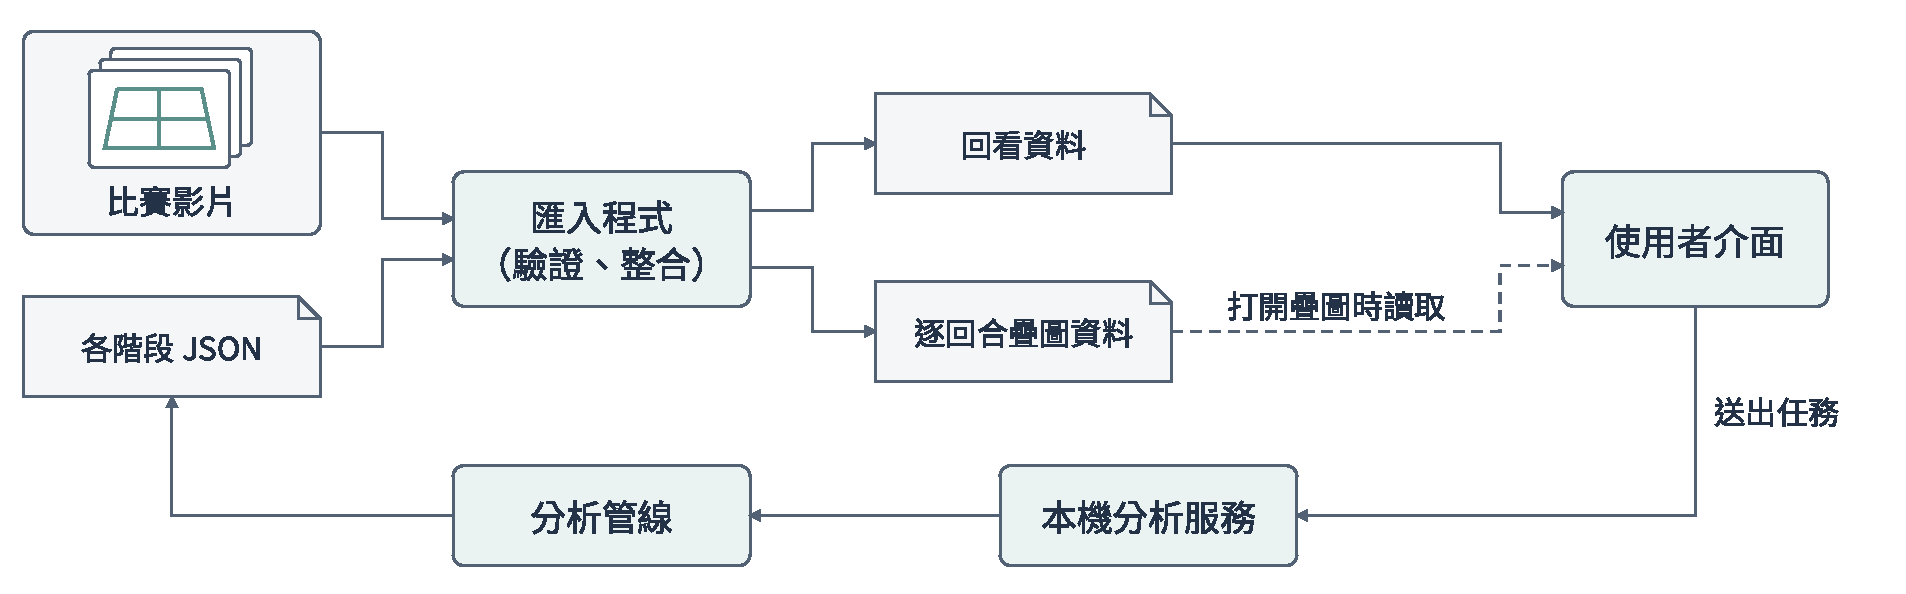
\includegraphics[scale=\flowscale]{ui-architecture.pdf}
  \caption{使用者介面實作架構}
  \label{fig:ui-architecture}
\end{figure}

\chapter{實驗結果}
\label{ch:experiments}

\section{資料集與重現方式}
\label{sec:datasets}

本章視覺模組的實驗共用下述影片庫。音訊模型另使用四場開發比賽與一場偵測器外部驗證，資料角色與結果另列於\secref{sec:exp-cheer}。資料集由 16 支 YouTube 羽球單打完整轉播構成，涵蓋 2018 至 2023 年的國際賽事。影片皆為 1920 $\times$ 1080，幀率為 25 或 30 fps，編碼格式包含 H.264、AV1 與 VP9。全部影片合計約 18.09 小時。為避免同一場比賽的資料同時出現在開發與評估中，資料以影片為單位切分為 7 場開發集與 9 場測試集（\tabref{tab:dataset-split}）。開發集用於設計與調整規則，測試集不參與開發，僅在完成後用於報告測試結果。由於其中 15 支影片來自 BWF 官方製作，跨轉播單位的泛化能力仍待後續驗證。

\begin{table}[H]
  \centering
  \caption{資料集切分}
  \label{tab:dataset-split}
  \begin{tabular}{|l|r|r|}
    \hline
    資料分割 & 影片數 & 影格數 \\ \hline
    開發集 & 7 & 852,297 \\ \hline
    測試集 & 9 & 851,704 \\ \hline
    合計 & 16 & 1,704,001 \\ \hline
  \end{tabular}
\end{table}

為使影格編號可被他人重現，\file{experiments/dataset/videos.json} 與 \file{videos.md} 記錄每支影片的 YouTube 來源、解析度、幀率、影格數、編碼、SHA-256 雜湊及影格指紋。下載影片後，應先放至 \texttt{matches/<代號>/input/}，並執行下列指令確認檔案與標記時所用影片一致：

\begin{Verbatim}
uv sync
uv run python experiments/dataset/verify_video.py --all
\end{Verbatim}

驗證程式依序檢查檔案雜湊、影格數／幀率／長度，以及固定影格的畫面指紋。即使檔案經重新壓縮，只要影格序列相同仍可通過指紋檢查。

各視覺模組的真值、標記與評分程式及逐場結果置於 \file{experiments/}，影片清單與驗證程式在 \file{experiments/dataset/}。音訊研究的程式與凍結文件另在 badminton-audio-highlight 儲存庫（\url{https://github.com/2026bmtproject/badminton-audio-highlight}，核對 commit \texttt{f72eb4c}），其 labels、features 與結果 JSON 未納入 Git 追蹤，來源雜湊與重現限制見 \file{experiments/audio_highlight/README.md}。

\section{各模組結果}
\label{sec:module-results}

\subsection{賽事影片分段}
\label{sec:exp-segmentation}

在 9 場未參與開發的比賽、670 個真值片段上，本模組在 IoU $\geq$ 0.9 下達到 Precision 98.37\%、Recall 98.96\%，邊界誤差中位數為 0 影格。16 場、1354 個片段的整體 F1 為 99.01\%，其中 11 場零錯誤。分段結果會直接決定下游分析範圍，因此本節分別驗證片段偵測、邊界精度，並分析所有失配案例。

真值、標記程式、評分程式與逐場結果皆公開於 \file{experiments/match_segmentation/}。

本模組的真值定義為「固定主機位之連續比賽畫面」的起訖影格，起訖兩端均包含。所有真值由同一位標記者完成。

\subsubsection{偵測準確率}

配對規則為 IoU $\geq$ 0.9、一對一，未配對的輸出段計為 FP、未配對的真值段計為 FN（\tabref{tab:seg-accuracy}）。

\begin{table}[H]
  \centering
  \small
  \caption{賽事影片分段的偵測準確率（\%）}
  \label{tab:seg-accuracy}
  \begin{tabular}{|l|r|r|r|r|r|r|r|r|}
    \hline
    範圍 & 真值 & 輸出 & 配對 & FP & FN & Precision & Recall & F1 \\ \hline
    開發集 & 684 & 687 & 681 & 6 & 3 & 99.13 & 99.56 & 99.34 \\ \hline
    測試集 & 670 & 674 & 663 & 11 & 7 & 98.37 & 98.96 & 98.66 \\ \hline
    合計 & 1354 & 1361 & 1344 & 17 & 10 & 98.75 & 99.26 & 99.01 \\ \hline
  \end{tabular}
\end{table}

16 場中有 11 場零錯誤，全部 27 筆失配集中在 5 支影片上。

\subsubsection{邊界精度}

誤差定義為「輸出 $-$ 真值」，單位為影格，只計算配對成功的段。起點為正代表系統比真值晚開始（切掉了開頭），終點為負代表系統比真值早結束（切掉了結尾）。

\begin{table}[H]
  \centering
  \small
  \caption{賽事影片分段的邊界誤差（影格）}
  \label{tab:seg-boundary}
  \begin{tabular}{|l|r|r|r|r|r|r|}
    \hline
    範圍 & 起點中位數 & 起點 MAE & 起點最大偏移 & 終點中位數 & 終點 MAE & 終點最大偏移 \\ \hline
    開發集 & +0.0 & 0.31 & +6 & +0.0 & 0.01 & $-3$ \\ \hline
    測試集 & +0.0 & 0.19 & +4 & +0.0 & 0.05 & $-10$ \\ \hline
    合計 & +0.0 & 0.26 & +6 & +0.0 & 0.03 & $-10$ \\ \hline
  \end{tabular}
\end{table}

1344 個配對段中沒有任何一段的邊界誤差超過 10 影格（\tabref{tab:seg-boundary}）。只要一個回合被完整切出來，它的邊界幾乎一定是準的。

\subsubsection{失敗案例與限制}

27 筆失配可歸為三類，且各自集中於特定影片（\tabref{tab:seg-failures}）。其中漏掉表示回合未被完整切出，多切則表示產生額外片段。

\begin{table}[H]
  \centering
  \small
  \caption{賽事影片分段的失配成因}
  \label{tab:seg-failures}
  \begin{tabularx}{\linewidth}{|L|r|r|>{\raggedright\arraybackslash}p{13em}|}
    \hline
    成因 & 多切 & 漏掉 & 影響的比賽 \\ \hline
    一、播報圖卡動畫把回合切成碎片 & 11 & 6 & TTY\_vs\_ASY\_2023、test1、test2、test3 \\ \hline
    二、全域亮度變化使跨片段篩選失效 & 1 & 2 & test4 \\ \hline
    三、門檻邊緣的高強度回合被切斷 & 5 & 2 & test6 \\ \hline
    合計 & 17 & 10 & \\ \hline
  \end{tabularx}
\end{table}

\textbf{一、播報圖卡動畫。}轉播在回合開始或結束時播放球員名條、比分卡等動畫，使 MAD 超過門檻，將回合切成碎片。動畫持續 3--6 秒，遠超過邊界精修可橋接的 12 影格，因此無法重新連接。

\textbf{二、全域亮度變化。}test4 開賽後前兩個回合整段消失。MAD 中位數與正常回合相近，表示門檻判斷本身沒有問題。真正失效的是跨片段一致性篩選。由於開賽初期場館燈光逐漸變亮，兩段畫面與其他回合雖然構圖相同，整體像素差卻明顯較高，因而被誤判為非比賽畫面。此類錯誤表現為整段消失，而非邊界偏移。

\textbf{三、門檻邊緣的高強度回合。}test6 有兩個高強度回合被切成數段，其中一個 11.4 秒的回合被切成三段。切斷處與保留區段的 MAD 均接近門檻，顯示球員劇烈移動使畫面差異在門檻附近波動。由於目前採用全片固定門檻，無法適應此類時間上的動態變化。

\textbf{已知但未在本資料集上觸發的限制。}若影片包含大量且相似的非比賽畫面，跨片段一致性篩選可能失效。系統亦假設存在穩定主機位，不適用於手持或多機快切影片。此外，16 支影片中有 15 支來自 BWF 官方製作，因此跨轉播單位的泛化能力尚未驗證。

\subsection{場地偵測}
\label{sec:exp-court}

在 9 場未參與開發的比賽、36 個球場外角上，本模組的角點定位誤差中位數為 2.79 像素，命中率 72.22\%，9 場中有 6 場四角全中。16 場、64 個外角的整體誤差中位數為 3.05 像素，命中率 76.56\%，11 場四角全中。

真值、標記程式、評分程式與逐場結果皆公開於 \file{experiments/court_detection/}。

\textbf{真值定義。}球場外緣是有寬度的白線，邊線與底線在外角交疊成一個小四邊形，本節稱為「角區」。標記時不直接點選角點，而是在合成圖上標出外框四條線各自的外緣與內緣，共 8 條邊緣，每個角區由相交的兩條底線邊緣與兩條邊線邊緣的 4 個交點構成。所有真值由同一位標記者完成。

\subsubsection{定位誤差}

誤差定義為偵測角點到角區中心的歐氏距離，單位為像素（\tabref{tab:court-error}）。

\begin{table}[H]
  \centering
  \small
  \caption{場地偵測的角點定位誤差（像素）}
  \label{tab:court-error}
  \begin{tabular}{|l|r|r|r|r|r|r|}
    \hline
    範圍 & 角數 & 遠端中位數 & 近端中位數 & 全部中位數 & 全部平均 & 全部最大 \\ \hline
    開發集 & 28 & 0.97 & 3.59 & 3.34 & 31.95 & 395.72 \\ \hline
    測試集 & 36 & 1.00 & 4.83 & 2.79 & 33.71 & 440.27 \\ \hline
    合計 & 64 & 1.00 & 3.62 & 3.05 & 32.94 & 440.27 \\ \hline
  \end{tabular}
\end{table}

中位數與平均值相差十倍，顯示誤差分布呈兩極，多數角點的誤差只有數像素，少數完全失敗的角則偏離數百像素。近端的像素誤差大於遠端，推測是鏡頭畸變使部分影片中近端底線彎曲造成。

\subsubsection{命中率}

命中定義為偵測角點落在角區內，或在角區外緣 2 像素容差內（\tabref{tab:court-hit}）。

\begin{table}[H]
  \centering
  \small
  \caption{場地偵測的命中率}
  \label{tab:court-hit}
  \begin{tabular}{|l|r|r|r|r|r|r|}
    \hline
    範圍 & 場數 & 遠端命中 & 近端命中 & 全部命中 & 命中率（\%） & 四角全中場數 \\ \hline
    開發集 & 7 & 11/14 & 12/14 & 23/28 & 82.14 & 5/7 \\ \hline
    測試集 & 9 & 14/18 & 12/18 & 26/36 & 72.22 & 6/9 \\ \hline
    合計 & 16 & 25/32 & 24/32 & 49/64 & 76.56 & 11/16 \\ \hline
  \end{tabular}
\end{table}

若不給容差、只計嚴格落在線寬內的角點，命中為 33/64（51.56\%）。有 16 個角點落在角區外緣 2 像素內，這類偏移已小於一條白線的寬度，在後續換算球場座標時可視為已對準。

\subsubsection{失敗案例與限制}

15 個未命中的角中，14 個來自同一根因，底線旁的地面廣告字樣在線段分群時與底線合併，導致代表線偏移（\tabref{tab:court-failures}）。

\begin{table}[H]
  \centering
  \small
  \caption{場地偵測的未命中成因}
  \label{tab:court-failures}
  \begin{tabularx}{\linewidth}{|L|r|r|l|}
    \hline
    成因 & 未命中角數 & 到角區中心距離 & 影響的比賽 \\ \hline
    底線被廣告字樣污染，收縮至內部矩形 & 8 & 17--440 px & CTC\_vs\_CL\_2019、test5 \\ \hline
    底線被廣告字樣污染，外擴至字樣邊緣 & 6 & 17--70 px & test8、test6 \\ \hline
    遠端角輕微偏移 & 1 & 10 px & ASG\_vs\_AA\_2020 \\ \hline
    合計 & 15 & & \\ \hline
  \end{tabularx}
\end{table}

\textbf{底線被廣告字樣污染。}轉播場館常在場地墊印製贊助商字樣，距底線僅約 10--40 像素。由於字樣位於球場遮罩內，白色字母會被視為線像素，並經霍夫轉換產生大量與底線平行的短線段，其方向正確，因此無法由消失點過濾排除。

將人工標記的真值四角直接代入同一套吻合度評分，test5 與 CTC\_vs\_CL\_2019 分別得到 0.825 與 0.922，明顯高於實際錯誤解的約 0.45，顯示評分本身能辨識正確解，問題主要發生在候選生成階段。

進一步僅修改線段分群方式並重跑 16 場，將合併距離由 14 像素縮為 6 像素，或改以最長線段為錨點並依線段長度加權擬合，命中數皆由 49/64 提升至 61/64，且上述四場全部恢復命中。由於這些修正是在觀察測試集失敗後才提出，因此不能將修正後結果視為未參與開發的測試結果，修正列為後續改進方向。

\textbf{系統無法察覺自身失敗。}三場四角全錯的比賽中，模組皆正常輸出四角與單應性，未標記為偵測失敗。原因是吻合度目前僅用於候選間比較，沒有絕對門檻判斷最佳解是否可信，因此錯誤結果仍會傳入下游模組。

\textbf{已知但未觸發的限制。}本模組假設機位固定，且球場大致位於畫面中央偏下，並從該區域取樣參考色。若機位偏移使取樣區域落在場外，顏色分割可能整體失效。

\subsection{擊球時刻偵測}
\label{sec:exp-events}

在 8 場未參與開發的比賽、6990 拍上，本模組在 $\pm$5 幀容差下達到 Precision 95.49\%、Recall 90.90\%，配對成功的擊球時間誤差中位數為 $-1$ 幀。14 場、12163 拍的整體 F1 為 92.10\%。

真值、評分程式與逐場結果皆公開於 \file{experiments/event_detection/}。

\textbf{真值來源。}本模組的真值取自公開資料集 ShuttleSet~\cite{shuttleset}（MIT 授權），以原檔形式收錄。16 場中有 14 場在 ShuttleSet 內，因此本節的開發集為 6 場、測試集為 8 場。答案幀原樣使用，唯一的調整是 \texttt{test5} 與 \texttt{test8}，我們取得的影片版本開頭多出一段賽前畫面，整體差了整數分鐘（+15000 與 +12000 幀），先予補回。

\textbf{評分範圍。}真值只涵蓋 ShuttleSet 收錄的回合，系統輸出也只存在於分段模組切出的片段內。因此只在兩者重疊的時間評分，以每個回合的第一拍到最後一拍（前後各放寬容差 tol）與片段取交集。全真值中有 97.9\% 落在評分範圍內。

\subsubsection{偵測準確率}

配對規則為偵測幀與答案幀相差 $\leq$ 5 幀、一對一，由相差最小者開始配對。未配對的偵測計為 FP，未配對的答案計為 FN（\tabref{tab:event-accuracy}）。

\begin{table}[H]
  \centering
  \small
  \caption{擊球時刻偵測的準確率（\%，容差 $\pm$5 影格）}
  \label{tab:event-accuracy}
  \begin{tabular}{|l|r|r|r|r|r|r|r|r|}
    \hline
    範圍 & 真值 & 輸出 & 配對 & FP & FN & Precision & Recall & F1 \\ \hline
    開發集 & 5173 & 4981 & 4605 & 376 & 568 & 92.45 & 89.02 & 90.70 \\ \hline
    測試集 & 6990 & 6654 & 6354 & 300 & 636 & 95.49 & 90.90 & 93.14 \\ \hline
    合計 & 12163 & 11635 & 10959 & 676 & 1204 & 94.19 & 90.10 & 92.10 \\ \hline
  \end{tabular}
\end{table}

容差放寬或收緊時的變化如\tabref{tab:event-tolerance}。

\begin{table}[H]
  \centering
  \small
  \caption{不同容差下的擊球時刻偵測準確率（\%，全部 14 場）}
  \label{tab:event-tolerance}
  \begin{tabular}{|r|r|r|r|}
    \hline
    容差（影格） & Precision & Recall & F1 \\ \hline
    3 & 89.07 & 84.16 & 86.54 \\ \hline
    5 & 94.19 & 90.10 & 92.10 \\ \hline
    10 & 95.68 & 92.65 & 94.14 \\ \hline
  \end{tabular}
\end{table}

\subsubsection{時間誤差}

誤差定義為「偵測 $-$ 答案」，單位為影格，只計算配對成功的擊球（\tabref{tab:event-timing}）。

\begin{table}[H]
  \centering
  \small
  \caption{擊球時刻偵測的時間誤差（影格）}
  \label{tab:event-timing}
  \begin{tabular}{|l|r|r|r|}
    \hline
    範圍 & 中位數 & 平均 & MAE \\ \hline
    開發集 & $-1$ & $-1.46$ & 1.80 \\ \hline
    測試集 & $-1$ & $-1.15$ & 1.55 \\ \hline
    合計 & $-1$ & $-1.28$ & 1.66 \\ \hline
  \end{tabular}
\end{table}

以毫秒計，整體誤差中位數為 $-40$ ms，MAE 為 64.6 ms。多數擊球被系統抓在真值前 1 至 2 影格，推測是因為本模組偵測的是軌跡轉折點，而人工標記的是球拍接觸的畫面。

\subsubsection{失敗案例與限制}

以下分析測試集的 636 個 FN 與 300 個 FP，根據失配前後 $\pm$5 影格的模組內部紀錄，將失配依成因分類（\tabref{tab:event-failures}）。

\begin{table}[H]
  \centering
  \small
  \caption{擊球時刻偵測的失配成因（測試集）}
  \label{tab:event-failures}
  \begin{tabular}{|l|r|r|}
    \hline
    成因 & FN & FP \\ \hline
    抓到但時間差 6--10 影格 & 192 & 148 \\ \hline
    遠端擊球在影像中沒有轉折 & 159 & — \\ \hline
    篩選與修剪規則誤刪 & 182 & — \\ \hline
    發球未產生候選 & 63 & — \\ \hline
    同一拍重複偵測 & — & 74 \\ \hline
    其他 & 40 & 78 \\ \hline
    合計 & 636 & 300 \\ \hline
  \end{tabular}
\end{table}

最大宗的失配為時間偏移，FN 的 30\%、FP 的 49\% 屬於系統已在正確位置附近偵測到，但與真值相差 6--10 影格，因此同一拍同時形成 FN 與 FP。將容差由 5 影格放寬至 10 影格後，F1 由 92.10\% 提升至 94.14\%，顯示部分誤差來自擊球時間定位差異。

FN 主要來自兩類。其一是遠端擊球缺乏軌跡轉折，部分遠端球員擊球時，球在影像中的運動方向未改變，僅速度微小改變，因此無法觸發以軌跡轉折為核心的候選訊號。其二是候選遭後續規則刪除，主要涉及同側去重、回合脈絡判斷與尾段修剪。

FP 則主要來自同一拍的重複偵測。同一擊球可能產生多個候選，若其擊球側判斷不同，現有去重規則無法合併。其餘補漏規則誤觸發與球體追蹤雜訊合計僅占少數。

本實驗的評分範圍只延伸至回合最後一拍後 5 影格，因此無法完整評估回合結束後落地彈跳造成的誤判，以及尾段修剪規則的實際效果。

\subsection{球種分類}
\label{sec:exp-strokes}

在 3 場 BST 未曾看過的比賽、1601 拍上，本模組的 8 類球種準確率為 87.38\%，Macro-F1 為 84.71\%，擊球者（上方／下方）準確率為 97.88\%。若把擊球時刻偵測漏掉的拍也算錯，端到端準確率為 78.99\%。

真值、評分程式與逐場結果皆公開於 \file{experiments/stroke_classification/}。

\textbf{真值來源。}本節與擊球時刻偵測使用同一份 ShuttleSet 真值，評分範圍與配對規則也完全相同。ShuttleSet 的 18 種球種先依 BST 訓練時的方式併為 12 類，再併為系統輸出的 8 類。

\textbf{BST 看過的比賽。}本模組使用的 BST 權重即以 ShuttleSet 訓練~\cite{bst}。依 BST 公開的切分，14 場中有 11 場屬於其訓練集，在這些比賽上量得的準確率可能偏高，只有 3 場未參與 BST 訓練。因此本節以這 3 場為主要結果，其餘 11 場僅作對照。

\subsubsection{分類準確率}

\begin{table}[H]
  \centering
  \small
  \caption{球種分類的準確率（\%）}
  \label{tab:stroke-accuracy}
  \begin{tabular}{|l|r|r|r|r|r|}
    \hline
    範圍 & 計分拍數 & 球種 Acc & Macro-F1 & 端到端 Acc & 擊球者 Acc \\ \hline
    \textbf{BST 沒看過（3 場）} & \textbf{1601} & \textbf{87.38} & \textbf{84.71} & \textbf{78.99} & \textbf{97.88} \\ \hline
    BST 看過（11 場） & 9333 & 88.32 & 86.36 & 80.06 & 98.02 \\ \hline
    合計（14 場） & 10934 & 88.18 & 86.22 & 79.90 & 98.00 \\ \hline
  \end{tabular}
\end{table}

BST 看過與沒看過的兩組只相差約 1 個百分點（\tabref{tab:stroke-accuracy}），可見在 BST 看過的比賽上量得的結果沒有明顯偏高。推測原因是 BST 訓練時的骨架與球軌跡由其原作者的流程產生，本系統則由自己的姿態與球體追蹤模組產生。

沒看過的 3 場各球種表現如\tabref{tab:stroke-per-class}。

\begin{table}[H]
  \centering
  \small
  \caption{各球種的分類表現（BST 沒看過的 3 場，\%）}
  \label{tab:stroke-per-class}
  \begin{tabular}{|l|r|r|r|r|}
    \hline
    球種 & 真值拍數 & Precision & Recall & F1 \\ \hline
    高遠球 & 531 & 92.28 & 90.02 & 91.13 \\ \hline
    發球 & 93 & 98.81 & 89.25 & 93.79 \\ \hline
    小球 & 387 & 95.03 & 88.89 & 91.86 \\ \hline
    平快球 & 136 & 59.63 & 70.59 & 64.65 \\ \hline
    殺球 & 174 & 87.85 & 91.38 & 89.58 \\ \hline
    切球 & 189 & 85.71 & 88.89 & 87.27 \\ \hline
    撲球 & 19 & 93.33 & 73.68 & 82.35 \\ \hline
    勾球 & 72 & 75.00 & 79.17 & 77.03 \\ \hline
  \end{tabular}
\end{table}

\subsubsection{上游影響}

為區分錯誤來自擊球時刻還是 BST 本身，另將擊球幀換成真值的擊球幀重跑一次球種分類，其他輸入（骨架、球軌跡、場地、權重）不變（\tabref{tab:stroke-upstream}）。

\begin{table}[H]
  \centering
  \small
  \caption{以系統偵測或真值擊球幀進行球種分類的比較（\%）}
  \label{tab:stroke-upstream}
  \begin{tabular}{|l|r|r|r|r|}
    \hline
    擊球幀 & 計分拍數 & 球種 Acc & Macro-F1 & 擊球者 Acc \\ \hline
    系統偵測 & 1601 & 87.38 & 84.71 & 97.88 \\ \hline
    真值 & 1771 & 88.54 & 84.98 & 98.54 \\ \hline
  \end{tabular}
\end{table}

即使擊球時刻完全正確，準確率也只提升 1.16 個百分點。

\subsubsection{失敗案例與限制}

沒看過的 3 場中共有 202 拍判錯，依重跑結果分類如\tabref{tab:stroke-failures}。

\begin{table}[H]
  \centering
  \small
  \caption{球種分類的錯誤成因（BST 沒看過的 3 場）}
  \label{tab:stroke-failures}
  \begin{tabular}{|l|r|}
    \hline
    成因 & 拍數 \\ \hline
    BST 本身判錯（換成真值擊球幀仍錯） & 146 \\ \hline
    擊球時刻所致（換成真值擊球幀即正確） & 48 \\ \hline
    判成未知球種 & 8 \\ \hline
    合計 & 202 \\ \hline
  \end{tabular}
\end{table}

BST 本身的錯誤集中在軌跡相近的球種之間。最多的是高遠球與平快球互判（49 + 26 拍），其次是小球與勾球（19 + 10 拍）和殺球與切球（14 + 10 拍）。

\subsection{歡呼偵測與精彩度分析}
\label{sec:exp-cheer}

\subsubsection{歡呼偵測資料集與評估方式}

歡呼偵測任務以 3 秒窗口為單位，資料來自四場開發比賽。每場以固定 seed 42 的 segment-diverse deterministic sampling 選取 100 個窗口，再由人工進行 blind labeling（\tabref{tab:cheer-dataset}）。標註允許 ambiguous；二元分類資料會排除 ambiguous，本次四場凍結資料沒有 ambiguous 樣本。

\begin{table}[H]
  \centering
  \small
  \caption{歡呼偵測的標註資料}
  \label{tab:cheer-dataset}
  \begin{tabular}{|l|r|r|r|}
    \hline
    比賽 & 歡呼 & 非歡呼 & 合計 \\ \hline
    \texttt{match\_001} & 33 & 67 & 100 \\ \hline
    \texttt{match\_002} & 31 & 69 & 100 \\ \hline
    \texttt{match\_003} & 55 & 45 & 100 \\ \hline
    \texttt{match\_004} & 31 & 69 & 100 \\ \hline
    合計 & 150 & 250 & 400 \\ \hline
  \end{tabular}
\end{table}

評估採 Leave-One-Match-Out（LOMO）：每一 fold 以三場共 300 個窗口訓練，剩餘一場的 100 個窗口作為測試資料。StandardScaler 只在該 fold 的訓練資料上 fitting，再套用到 held-out match。相較隨機拆分窗口，此方法以 match ID 隔離訓練與測試資料，避免同場相鄰窗口分散到兩邊；目前缺少完整賽事來源對照，尚不能據此宣稱跨轉播商的獨立性，但四場比賽仍不足以證明模型可普遍泛化。

\subsubsection{跨比賽歡呼偵測結果}

\begin{table}[H]
  \centering
  \small
  \caption{歡呼偵測的逐場交叉驗證結果（LOMO）}
  \label{tab:cheer-lomo}
  \begin{tabular}{|l|r|r|r|r|r|r|l|}
    \hline
    測試比賽 & Accuracy & Precision & Recall & F1 & ROC-AUC & AP & \texttt{[[TN,FP],[FN,TP]]} \\ \hline
    \texttt{match\_001} & 0.940 & 0.966 & 0.848 & 0.903 & 0.990 & 0.983 & \texttt{[[66,1],[5,28]]} \\ \hline
    \texttt{match\_002} & 0.870 & 1.000 & 0.581 & 0.735 & 0.934 & 0.904 & \texttt{[[69,0],[13,18]]} \\ \hline
    \texttt{match\_003} & 0.870 & 0.850 & 0.927 & 0.887 & 0.958 & 0.968 & \texttt{[[36,9],[4,51]]} \\ \hline
    \texttt{match\_004} & 0.850 & 0.711 & 0.871 & 0.783 & 0.947 & 0.907 & \texttt{[[58,11],[4,27]]} \\ \hline
    Macro 平均 & 0.883 & 0.882 & 0.807 & 0.827 & 0.957 & 0.940 & — \\ \hline
  \end{tabular}
\end{table}

四場 LOMO 的 macro Accuracy 為 0.883、macro F1 為 0.827、macro ROC-AUC 為 0.957（\tabref{tab:cheer-lomo}）。0.957 是 ROC-AUC，不是 95.7\% accuracy。各場 Brier score、Log Loss 與 ECE 顯示 score calibration behavior 存在差異；本研究沒有進行 recalibration，門檻仍固定為 0.5，因此分類器輸出不視為已校準機率。

校準診斷採 10 個等寬 bins，每場 100 個窗口；結果只用於檢查分數分布，沒有重新擬合校準器（\tabref{tab:cheer-calibration}）。

\begin{table}[H]
  \centering
  \small
  \caption{歡呼分類器的校準診斷}
  \label{tab:cheer-calibration}
  \begin{tabular}{|l|r|r|r|}
    \hline
    比賽 & Brier score & Log Loss & ECE \\ \hline
    \texttt{match\_001} & 0.038 & 0.125 & 0.037 \\ \hline
    \texttt{match\_002} & 0.112 & 0.480 & 0.131 \\ \hline
    \texttt{match\_003} & 0.101 & 0.340 & 0.096 \\ \hline
    \texttt{match\_004} & 0.121 & 0.528 & 0.132 \\ \hline
  \end{tabular}
\end{table}

另以未參與上述四場訓練的 \texttt{match\_005} 進行偵測器外部驗證。100 個窗口包含 34 個正例與 66 個負例，Accuracy 為 0.840，Precision、Recall 與 F1 均為 0.765，ROC-AUC 為 0.930，Average Precision（AP）為 0.862。\texttt{match\_005} 只對偵測器是 untouched external validation；它後續又參與強度與 segment 聚合方法的開發，因此不能用來證明後兩者的 external generalization。

為比較特徵路線，研究亦評估 RMS、YAMNet 原生 \texttt{Cheering} 分數、YAMNet crowd-combination 分數與 YAMNet embedding + Logistic Regression（\tabref{tab:cheer-features}）：

\begin{table}[H]
  \centering
  \small
  \caption{不同歡呼特徵路線的比較（LOMO）}
  \label{tab:cheer-features}
  \begin{tabular}{|l|r|r|}
    \hline
    方法 & LOMO ROC-AUC & LOMO AP \\ \hline
    RMS & 0.920 & 0.876 \\ \hline
    YAMNet \texttt{Cheering} 分數 & 0.839 & 0.750 \\ \hline
    YAMNet crowd-combination & 0.857 & 0.757 \\ \hline
    \textbf{YAMNet embedding + Logistic Regression} & \textbf{0.957} & \textbf{0.940} \\ \hline
  \end{tabular}
\end{table}

此比較支持 production 採用 embedding + Logistic Regression，而非直接使用 YAMNet 原生類別分數。這些數字是描述性比較，未執行 threshold tuning 或統計顯著性檢定。

最終部署模型再用四場的全部 400 個窗口 fitting scaler 與分類器；此 final fit 不是新的測試結果。LOMO 的 scaler 則各自只用當 fold 的 300 個訓練窗口。模型權重與 feature dataset hashes 記錄於 \file{models/yamnet_mean_lr_v1/metadata.json}。

\subsubsection{歡呼強度方法選擇}

強度實驗使用 \texttt{match\_005} 中 34 個已確認的歡呼窗口。單一主要標註者在不查看候選特徵值的情況下完成 60 組配對比較，其中 39 組有明確較強者、21 組平手、0 組無法判斷（\tabref{tab:cheer-intensity}）。

\begin{table}[H]
  \centering
  \small
  \caption{歡呼強度候選方法與人工配對比較的一致性}
  \label{tab:cheer-intensity}
  \begin{tabular}{|l|r|r|r|}
    \hline
    候選方法 & Strict concordance & Coverage & Tie-adjusted concordance \\ \hline
    \texttt{log\_rms\_db} & 0.692 & 1.000 & 0.692 \\ \hline
    \texttt{cheer\_probability} & 0.667 & 1.000 & 0.667 \\ \hline
    \texttt{temporal\_occupancy} & 0.457 & 0.897 & 0.462 \\ \hline
    \texttt{relative\_loudness\_db} & 0.436 & 1.000 & 0.436 \\ \hline
  \end{tabular}
\end{table}

\texttt{log\_rms\_db} 的描述性 concordance 最高且 coverage 完整，也能將分類器信心與聲學強度分開，因此選為凍結的 intensity feature。然而，它與 \texttt{cheer\_probability} 的差距不大，實驗沒有顯著性檢定，而且同一窗口會出現在多組配對中，60 組觀察值並不獨立。因此，此結果不能解讀為 \texttt{log\_rms\_db} 在其他資料上必然優於分類器分數。

\subsubsection{Segment 聚合方法選擇}
\label{sec:exp-aggregation}

Segment 聚合實驗使用 \texttt{match\_005} 的 106 個 segments、1142 個重疊窗口與 420 個 detector-positive 窗口。人工 segment detection 標註包含 75 個 cheer 與 31 個 no-cheer segments；尖峰強度實驗則由 60 組人工配對構成，其中 45 組有明確結果、15 組平手（\tabref{tab:cheer-aggregation}）。

\begin{table}[H]
  \centering
  \small
  \caption{片段層級聚合方法的比較}
  \label{tab:cheer-aggregation}
  \begin{tabularx}{\linewidth}{|l|r|r|r|>{\raggedleft\arraybackslash}X|}
    \hline
    方法 & 偵測 ROC-AUC & 偵測 AP & Peak-pair concordance & 移除單一窗口的最大分數差異，中位數 / Q95（偵測） \\ \hline
    mean & 0.624 & 0.749 & 0.600 & 0.066 / 0.144 \\ \hline
    max & 0.710 & 0.862 & 0.711 & 0.005 / 0.489 \\ \hline
    p95 linear & 0.718 & 0.863 & 0.711 & 0.021 / 0.391 \\ \hline
    top-2 mean & 0.719 & 0.867 & 0.733 & 0.026 / 0.430 \\ \hline
    top-3 mean & 0.717 & 0.862 & 0.733 & 0.134 / 0.333 \\ \hline
  \end{tabularx}
\end{table}

Max 與 p95 是預先指定的主要候選，mean 是參考方法，top-2 與 top-3 則是 secondary diagnostics。雖然 top-2 與 top-3 的部分 point estimates 較高，但不能在看到結果後將 secondary diagnostics 改稱勝出方法；各候選也沒有統計上的 winner claim。

最終選擇 linear p95 是工程折衷，而非實驗證明它是最佳聚合器。P95 保留對局部尖峰的敏感度，其人工 detection 與 peak-pair 表現和 max 接近；在移除單一窗口的診斷中，p95 的極端尾端敏感度又低於 max。因此，正式系統以 p95 同時聚合窗口機率與非空值強度。

本節數字逐項核對既有研究 JSON，未重跑模型或重新標註。Intensity strict concordance 以特徵可區分的人工明確配對為分母，coverage 表示明確配對中可區分的比例；人工平手不納入該分母。Segment peak-pair 比較的 45 組明確配對皆可由各候選區分。來源 commit、JSON hashes 與重現限制見 \file{experiments/audio_highlight/README.md}。

\section{端到端結果}
\label{sec:end-to-end}

本節時間表沿用既有七個視覺階段的量測，未計入本次新增說明的音訊量測、精彩度排序、身分對應與賽評生成成本，不能用作完整十一階段流程的耗時。

在 5 支影片中，回合總長 1.63 小時，整條管線從空快取開始執行共耗時 4.42 小時。主要計算只作用在回合片段，因此處理時間以回合總長衡量，E2E 時間為回合總長的 2.71 倍，扣除比分辨識等待 Gemini API 的時間後為 1.96 倍。

量測程式、環境紀錄與逐場結果皆公開於 \file{experiments/end_to_end/}。

\textbf{量測方式。}每場另建只含原始影片的資料夾，所有 stage 都從空快取開始實際執行。E2E 時間由外層計時包住 runner 取得，各 stage 時間取自各自的狀態紀錄。比分辨識的耗時主要取決於 API 速率上限而非本機效能，因此另列扣除該 stage 後的「本機時間」。賽評不在預設管線內，不列入。測試環境為 Windows 11 與 RTX 3060 Ti（8 GB）。

\subsection{處理時間}

\begin{table}[H]
  \centering
  \small
  \caption{端到端處理時間}
  \label{tab:e2e-time}
  \begin{tabularx}{\linewidth}{|l|l|>{\raggedleft\arraybackslash}X|>{\raggedleft\arraybackslash}X|>{\raggedleft\arraybackslash}X|>{\raggedleft\arraybackslash}X|>{\raggedleft\arraybackslash}X|>{\raggedleft\arraybackslash}X|}
    \hline
    比賽 & 編碼／幀率 & 片長（分） & 回合總長（分） & E2E（分） & 本機（分） & E2E ÷ 回合總長 & 本機 ÷ 回合總長 \\ \hline
    test1 & VP9／25 & 8.2 & 5.3 & 19.5 & 10.8 & 3.65 & 2.02 \\ \hline
    test5 & H.264／25 & 57.3 & 15.0 & 38.0 & 26.8 & 2.53 & 1.79 \\ \hline
    test4 & VP9／25 & 71.9 & 18.3 & 42.5 & 32.9 & 2.32 & 1.80 \\ \hline
    test2 & H.264／25 & 100.9 & 31.4 & 74.9 & 57.2 & 2.38 & 1.82 \\ \hline
    TTY\_vs\_ASY\_2023 & AV1／30 & 94.0 & 27.8 & 90.1 & 63.8 & 3.24 & 2.29 \\ \hline
    合計 & & 332.3 & 97.8 & 264.9 & 191.5 & 2.71 & 1.96 \\ \hline
  \end{tabularx}
\end{table}

以回合總長正規化後，本機時間在 3 場 25 fps 的完整比賽間相當一致（\tabref{tab:e2e-time}）。TTY\_vs\_ASY\_2023 為 30 fps，同樣長度的回合多出 20\% 影格，加上 AV1 解碼較重，比例較其他場高。

\subsection{時間分布}

\begin{table}[H]
  \centering
  \small
  \caption{各階段佔總處理時間的比例}
  \label{tab:e2e-breakdown}
  \begin{tabular}{|l|r|}
    \hline
    stage & 佔比 \\ \hline
    \texttt{shuttle\_tracking} & 34.6\% \\ \hline
    \texttt{score\_recognition} & 27.8\% \\ \hline
    \texttt{pose} & 27.6\% \\ \hline
    \texttt{match\_segmentation} & 7.0\% \\ \hline
    其餘 6 個 stage & 3.0\% \\ \hline
  \end{tabular}
\end{table}

前三個 stage 合計約 90\%（\tabref{tab:e2e-breakdown}）。球體追蹤與骨架追蹤的耗時與回合影格數成正比，在 25 fps 的影片上分別約為每影格 33 ms 與 27--31 ms。

\subsection{限制}

\begin{itemize}
  \item \textbf{偶發崩潰。}TTY\_vs\_ASY\_2023 第一次執行時，骨架追蹤在開始約 11 秒後發生原生程式崩潰，重跑後正常完成，表中為重跑結果。原因尚未查明。
  \item \textbf{量測範圍。}每場只執行一次，未估計量測變異，也只在單一硬體上測試。
\end{itemize}

\subsection{應用於延遲直播的可能性}

以上結果顯示，系統稍加調整後，或許能用於延遲一段時間播出的比賽直播。本機計算時間約為回合長度的 1.8--2.3 倍，而完整比賽中回合只佔播出時間的 25--31\%，平均而言處理速度跟得上播出，因此若改為逐回合處理，計算量不會隨比賽進行而累積。以本機時間約為回合長度的 1.8--2.3 倍估算，最長的 55.7 秒回合約需 2 分鐘以上為依本次量測推估的結果，尚未實作驗證。

\chapter{討論與結論}
\label{ch:conclusion}

\section{系統優點與限制}
\label{sec:strengths-limitations}

\textbf{優點。}系統的設計特點已於\secref{sec:contributions}說明，\chapref{ch:experiments}的實驗進一步證實了自動化的上游步驟在未參與開發的比賽上依然有效。賽事影片分段與擊球時刻偵測在測試集上的 F1 分別為 98.66\% 與 93.14\%，與開發集的 99.34\% 與 90.70\% 相當。

\textbf{限制。}

\begin{enumerate}
  \item \textbf{依賴對轉播形式的假設。}多數規則建立在 BWF 轉播的慣例上，固定俯拍主機位、球場大致位於畫面中央偏下，且只處理單打。在符合假設的影片上準確率高，但假設一旦不成立，模組可能直接失效而非逐漸退化，例如手持或多機快切的影片無法分段，機位偏移可能使場地顏色分割整體失效。資料集 16 支影片中有 15 支來自 BWF，這類情況在實驗中幾乎沒有機會出現，此部分泛化能力尚未驗證。
  \item \textbf{規則有過擬合的跡象。}分段、場地偵測與擊球偵測都包含許多依開發集調整的門檻與規則。分段與擊球偵測在測試集上的表現與開發集相近，但場地偵測的命中率由開發集的 82.14\% 降至測試集的 72.22\%，失敗幾乎都來自開發時未遇過的底線廣告字樣。規則愈多，遇到新場館或新轉播風格時愈可能出現未預期的交互作用。本系統以規則取代標記訓練，避開了\chapref{ch:related-work}指出的標記成本，但依開發集調出的門檻同樣可能隨轉播形式失準。在資料集以 BWF 轉播為主的情況下，尚無法證明此路線比學習式方法更能泛化。
  \item \textbf{無法察覺自身失敗。}場地偵測在三場四角全錯的比賽中仍正常輸出，分段也可能整段漏掉回合而不留任何警示。系統缺乏信心度判斷，目前只能靠使用者回看時發現並手動修正。
  \item \textbf{外部依賴與處理速度。}比分辨識與賽評依賴 Gemini API，前者受速率上限影響，約占處理時間的 28\%。處理時間約需回合總長的 2.7 倍，且未含音訊、身分對應與賽評。若要用於延遲直播，仍需改為逐回合處理，並降低對 API 的依賴。
  \item \textbf{音訊支線的證據有限。}歡呼偵測只以四場開發比賽與一場外部驗證評估，不足以涵蓋不同轉播商、場館、觀眾規模與混音方式。該外部驗證場之後又參與了強度與聚合方法的開發，而這兩項的人工比較樣本少、只有單一標註者，因此只足以支持第一版的方法選擇。此外，歡呼強度是單場內的相對排名，不能跨比賽比較。歡呼也不等同回合的技術品質，可能同時受比分、球星或爭議影響，加上精彩度分數的 0.5／0.5 權重沒有人工排序真值支持，只能作為補充的排序訊號。
  \item \textbf{缺乏使用者評估。}介面與賽評目前只經開發者自行使用，沒有對教練、球員等目標使用者進行可用性測試，本報告也未量化評估生成賽評的品質，系統實際能減少多少人工逐拍標記的工作仍待驗證。
\end{enumerate}

\section{結論}
\label{sec:conclusion}

本專題建立了一套全自動的羽球單打轉播分析系統。系統輸出每個主機位比賽片段的起訖時間與比分、每一拍的擊球影格、擊球者與球種，以及雙方球員的骨架、球場範圍與羽球軌跡，並據此產生精彩片段排序與賽評。既有方法所依賴的比賽片段起訖、球場範圍與擊球時刻，以及既有系統未曾直接讀取的計分板比分，在本系統中都已自動取得。在未參與開發的比賽上，賽事影片分段與擊球時刻偵測的 F1 分別達 98.66\% 與 93.14\%，管線已能在真實轉播影片上從頭到尾自動完成。最弱的一環是場地偵測，測試集的命中率為 72.22\%，未命中的角幾乎都源於底線旁的廣告字樣。

綜合各模組的實驗結果，上游步驟自動化之後，球種資料的瓶頸落在兩處。一是 BST 本身，將擊球幀換成真值後準確率只提升 1.16 個百分點，未看過的 3 場中 202 拍錯誤有 146 拍來自 BST。二是擊球時刻偵測的召回率，漏掉的拍無從分類，使端到端準確率比單看分類低約 8 個百分點。此外，系統無法察覺自身的失敗，場地偵測在三場四角全錯的比賽中仍正常輸出，錯誤會靜默傳入下游，目前只能靠人工回看發現。因此，除了提升單一模組的準確率，讓系統能判斷自身輸出是否可信同樣重要。

未來工作將針對上述限制展開。首先，蒐集非 BWF 轉播與更多場館的影片，驗證並改善泛化能力，同時為各模組加入信心度估計，在輸出可疑時提示使用者回看。其次，降低對外部 API 的依賴並改為逐回合處理，實現延遲直播的應用。此外，為比分辨識與球員身分對應建立真值並量化評估，擴充歡呼偵測資料，並建立精彩度的人工排序真值。最後，對教練與球員進行使用者研究，量化評估系統與生成賽評的實際效益。

\appendix
\chapter{人工智慧的使用}
\label{app:ai-usage}

\section{開發過程中的生成式 AI}

\textbf{使用的工具。}主要使用 Claude Code（Claude Opus 4.8、5.5），讓模型直接在專案目錄中讀寫程式與文件；另以 ChatGPT（Terra 5.6）作為不同來源的第二個模型，用於討論與交叉檢查。

\textbf{程式。}系統的程式碼幾乎全由 AI 撰寫。組員負責決定架構與設計，包括模組切分、階段之間的資料契約、採用哪些既有模型、實驗的評估方式，以及介面的互動與視覺設計，實作則交給 AI。實際流程通常是先請 AI 提出方案而不動手，由組員取捨後再實作，完成後由 AI 列出需要人工確認的項目，組員實際操作系統檢查，確認無誤才提交版本。

\textbf{研究。}AI 用於搜尋文獻與導讀論文，例如整理 BST 在 ShuttleSet 上的資料切分方式，以確認哪些比賽未參與其訓練。也用於部分演算法的優化、以小型實驗驗證想法是否可行，以及把中間結果視覺化，例如將骨架、軌跡與擊球時刻疊回影片逐幀檢視。

\textbf{報告與展示。}AI 參與了討論章節的內容整理、全文順稿與排版，並撰寫報告圖片的生成程式。專題競賽的影片分鏡、模組介紹動畫的程式與海報版面規劃也由 AI 協助。報告中的數據皆來自實驗程式的輸出，並非由 AI 生成。

\section{確保正確性的做法}

AI 產出的程式與文字可能看似合理卻有錯，因此我們依影響程度採取不同的檢查方式：

\begin{enumerate}
  \item \textbf{評分程式由人閱讀。}實驗的評分程式決定報告中所有準確率數字，因此要求 AI 以最直白的寫法撰寫，並由組員自行讀過確認邏輯。其他必要的程式也同樣自行閱讀。
  \item \textbf{以不同模型交叉檢查。}重要的程式與文件會交由另一個模型審查。例如第二個模型在審查分段實驗時發現，標註工具輸出的 1354 筆真值，其秒數欄位全部少算一幀。
  \item \textbf{視覺化檢查。}不只看程式回報的數字，而是把結果疊回影片或畫成圖，以人眼確認是否合理，許多錯誤是在這一步才發現的。
  \item \textbf{標出依據。}要求 AI 在提出結論時附上依據，例如程式的檔案與行號、實驗輸出的檔案或原始論文的段落，方便回頭查證。
  \item \textbf{重點驗證結果。}關鍵數字重新執行評分程式確認，修改模組後也以既有的評估結果作為回歸檢查，確認沒有退步。
\end{enumerate}

AI 大幅縮短了實作所需的時間，讓小組能把心力放在設計與驗證上。代價是組員對部分實作細節並不熟悉，因此我們把人工閱讀集中在評分程式這類直接影響結論的部分。

\chapter{音訊實驗來源與待補資料}
\label{app:audio-sources}

模型、資料角色、指標來源、JSON hashes、實作對照與重現限制見 \file{experiments/audio_highlight/README.md}。待補內容包含 \texttt{match\_001} 至 \texttt{match\_004} 的真實賽事來源、完整 cheer／no-cheer 標註規範、多標註者一致性，以及 labels／features／結果的可重現封存。這些缺口不由比賽資料夾名稱或模型輸出推導。


\printbibliography[heading=bibintoc, title={參考文獻}]

\end{document}
